% Options for packages loaded elsewhere
\PassOptionsToPackage{unicode}{hyperref}
\PassOptionsToPackage{hyphens}{url}
%
\documentclass[
  letterpaper,
]{scrbook}

\usepackage{amsmath,amssymb}
\usepackage{iftex}
\ifPDFTeX
  \usepackage[T1]{fontenc}
  \usepackage[utf8]{inputenc}
  \usepackage{textcomp} % provide euro and other symbols
\else % if luatex or xetex
  \usepackage{unicode-math}
  \defaultfontfeatures{Scale=MatchLowercase}
  \defaultfontfeatures[\rmfamily]{Ligatures=TeX,Scale=1}
\fi
\usepackage{lmodern}
\ifPDFTeX\else  
    % xetex/luatex font selection
\fi
% Use upquote if available, for straight quotes in verbatim environments
\IfFileExists{upquote.sty}{\usepackage{upquote}}{}
\IfFileExists{microtype.sty}{% use microtype if available
  \usepackage[]{microtype}
  \UseMicrotypeSet[protrusion]{basicmath} % disable protrusion for tt fonts
}{}
\makeatletter
\@ifundefined{KOMAClassName}{% if non-KOMA class
  \IfFileExists{parskip.sty}{%
    \usepackage{parskip}
  }{% else
    \setlength{\parindent}{0pt}
    \setlength{\parskip}{6pt plus 2pt minus 1pt}}
}{% if KOMA class
  \KOMAoptions{parskip=half}}
\makeatother
\usepackage{xcolor}
\usepackage[left=1in,marginparwidth=2.0666666666667in,textwidth=4.1333333333333in,marginparsep=0.3in]{geometry}
\setlength{\emergencystretch}{3em} % prevent overfull lines
\setcounter{secnumdepth}{5}
% Make \paragraph and \subparagraph free-standing
\ifx\paragraph\undefined\else
  \let\oldparagraph\paragraph
  \renewcommand{\paragraph}[1]{\oldparagraph{#1}\mbox{}}
\fi
\ifx\subparagraph\undefined\else
  \let\oldsubparagraph\subparagraph
  \renewcommand{\subparagraph}[1]{\oldsubparagraph{#1}\mbox{}}
\fi

\usepackage{color}
\usepackage{fancyvrb}
\newcommand{\VerbBar}{|}
\newcommand{\VERB}{\Verb[commandchars=\\\{\}]}
\DefineVerbatimEnvironment{Highlighting}{Verbatim}{commandchars=\\\{\}}
% Add ',fontsize=\small' for more characters per line
\newenvironment{Shaded}{}{}
\newcommand{\AlertTok}[1]{\textcolor[rgb]{1.00,0.33,0.33}{\textbf{#1}}}
\newcommand{\AnnotationTok}[1]{\textcolor[rgb]{0.42,0.45,0.49}{#1}}
\newcommand{\AttributeTok}[1]{\textcolor[rgb]{0.84,0.23,0.29}{#1}}
\newcommand{\BaseNTok}[1]{\textcolor[rgb]{0.00,0.36,0.77}{#1}}
\newcommand{\BuiltInTok}[1]{\textcolor[rgb]{0.84,0.23,0.29}{#1}}
\newcommand{\CharTok}[1]{\textcolor[rgb]{0.01,0.18,0.38}{#1}}
\newcommand{\CommentTok}[1]{\textcolor[rgb]{0.42,0.45,0.49}{#1}}
\newcommand{\CommentVarTok}[1]{\textcolor[rgb]{0.42,0.45,0.49}{#1}}
\newcommand{\ConstantTok}[1]{\textcolor[rgb]{0.00,0.36,0.77}{#1}}
\newcommand{\ControlFlowTok}[1]{\textcolor[rgb]{0.84,0.23,0.29}{#1}}
\newcommand{\DataTypeTok}[1]{\textcolor[rgb]{0.84,0.23,0.29}{#1}}
\newcommand{\DecValTok}[1]{\textcolor[rgb]{0.00,0.36,0.77}{#1}}
\newcommand{\DocumentationTok}[1]{\textcolor[rgb]{0.42,0.45,0.49}{#1}}
\newcommand{\ErrorTok}[1]{\textcolor[rgb]{1.00,0.33,0.33}{\underline{#1}}}
\newcommand{\ExtensionTok}[1]{\textcolor[rgb]{0.84,0.23,0.29}{\textbf{#1}}}
\newcommand{\FloatTok}[1]{\textcolor[rgb]{0.00,0.36,0.77}{#1}}
\newcommand{\FunctionTok}[1]{\textcolor[rgb]{0.44,0.26,0.76}{#1}}
\newcommand{\ImportTok}[1]{\textcolor[rgb]{0.01,0.18,0.38}{#1}}
\newcommand{\InformationTok}[1]{\textcolor[rgb]{0.42,0.45,0.49}{#1}}
\newcommand{\KeywordTok}[1]{\textcolor[rgb]{0.84,0.23,0.29}{#1}}
\newcommand{\NormalTok}[1]{\textcolor[rgb]{0.14,0.16,0.18}{#1}}
\newcommand{\OperatorTok}[1]{\textcolor[rgb]{0.14,0.16,0.18}{#1}}
\newcommand{\OtherTok}[1]{\textcolor[rgb]{0.44,0.26,0.76}{#1}}
\newcommand{\PreprocessorTok}[1]{\textcolor[rgb]{0.84,0.23,0.29}{#1}}
\newcommand{\RegionMarkerTok}[1]{\textcolor[rgb]{0.42,0.45,0.49}{#1}}
\newcommand{\SpecialCharTok}[1]{\textcolor[rgb]{0.00,0.36,0.77}{#1}}
\newcommand{\SpecialStringTok}[1]{\textcolor[rgb]{0.01,0.18,0.38}{#1}}
\newcommand{\StringTok}[1]{\textcolor[rgb]{0.01,0.18,0.38}{#1}}
\newcommand{\VariableTok}[1]{\textcolor[rgb]{0.89,0.38,0.04}{#1}}
\newcommand{\VerbatimStringTok}[1]{\textcolor[rgb]{0.01,0.18,0.38}{#1}}
\newcommand{\WarningTok}[1]{\textcolor[rgb]{1.00,0.33,0.33}{#1}}

\providecommand{\tightlist}{%
  \setlength{\itemsep}{0pt}\setlength{\parskip}{0pt}}\usepackage{longtable,booktabs,array}
\usepackage{calc} % for calculating minipage widths
% Correct order of tables after \paragraph or \subparagraph
\usepackage{etoolbox}
\makeatletter
\patchcmd\longtable{\par}{\if@noskipsec\mbox{}\fi\par}{}{}
\makeatother
% Allow footnotes in longtable head/foot
\IfFileExists{footnotehyper.sty}{\usepackage{footnotehyper}}{\usepackage{footnote}}
\makesavenoteenv{longtable}
\usepackage{graphicx}
\makeatletter
\def\maxwidth{\ifdim\Gin@nat@width>\linewidth\linewidth\else\Gin@nat@width\fi}
\def\maxheight{\ifdim\Gin@nat@height>\textheight\textheight\else\Gin@nat@height\fi}
\makeatother
% Scale images if necessary, so that they will not overflow the page
% margins by default, and it is still possible to overwrite the defaults
% using explicit options in \includegraphics[width, height, ...]{}
\setkeys{Gin}{width=\maxwidth,height=\maxheight,keepaspectratio}
% Set default figure placement to htbp
\makeatletter
\def\fps@figure{htbp}
\makeatother

%% Packages
\usepackage[russian, english]{babel}
\usepackage[default]{droidserif}
\usepackage[defaultsans]{droidsans}

\usepackage{xcolor}
\usepackage{soul}
\usepackage{amsmath, amsfonts}


\newcommand{\const}{\text{const}}
\newcommand{\lp}{\left(}
\newcommand{\rp}{\right)}
\newcommand{\lb}{\left[}
\newcommand{\rb}{\right]}

\newcommand*\circled[1]{\tikz[baseline=(char.base)]{
            \node[shape=circle,draw,inner sep=2pt] (char) {#1};}}

%% Logic
\newcommand{\xor}{\,\text{XOR}\,}

%% Number sets
\newcommand{\setN}{\mathbb{N}}
\newcommand{\setNo}{\mathbb{N}_{0}}
\newcommand{\setZ}{\mathbb{Z}}
\newcommand{\setQ}{\mathbb{Q}}
\newcommand{\setR}{\mathbb{R}}
\newcommand{\setC}{\mathbb{C}}

%% Linear Algebra
\newcommand{\vm}[1]{\mathbf{#1}} %% vectors and matrices

%% Probability, Random Vars
\newcommand{\alg}[1]{\mathcal{#1}}
\newcommand{\prob}{\mathbb{P}}
\newcommand{\expect}{\mathbb{E}}
\newcommand{\disp}{\mathbb{D}}
\newcommand{\var}{\text{var}}
\newcommand{\cov}{\text{cov}}
\newcommand{\cor}{\text{cor}}
\newcommand{\se}{\text{se}}
\newcommand{\sd}{\text{sd}}
\newcommand{\iid}{\text{i.i.d.}}

\newsavebox{\MBox}
\newcommand{\Cline}[2][red]{{\sbox\MBox{$#2$}%
  \rlap{\usebox\MBox}\color{#1}\rule[-1.2\dp\MBox]{\wd\MBox}{0.5pt}}}

%% Distributions
\newcommand{\norm}{\mathcal{N}}

%% Other
\newcommand{\defin}{\overset{\text{def}}{=}}
\newcommand{\sgn}{\mathrm{sgn}}

%% Trig
\newcommand{\artanh}{\text{artanh}}

%% Stats
\newcommand{\median}{\text{median}}
\newcommand{\mean}{\mathbb{M}}
\newcommand{\skewness}{\text{skew}}
\newcommand{\kurtosis}{\text{kurt}}
\makeatletter
\@ifpackageloaded{tcolorbox}{}{\usepackage[skins,breakable]{tcolorbox}}
\@ifpackageloaded{fontawesome5}{}{\usepackage{fontawesome5}}
\definecolor{quarto-callout-color}{HTML}{909090}
\definecolor{quarto-callout-note-color}{HTML}{0758E5}
\definecolor{quarto-callout-important-color}{HTML}{CC1914}
\definecolor{quarto-callout-warning-color}{HTML}{EB9113}
\definecolor{quarto-callout-tip-color}{HTML}{00A047}
\definecolor{quarto-callout-caution-color}{HTML}{FC5300}
\definecolor{quarto-callout-color-frame}{HTML}{acacac}
\definecolor{quarto-callout-note-color-frame}{HTML}{4582ec}
\definecolor{quarto-callout-important-color-frame}{HTML}{d9534f}
\definecolor{quarto-callout-warning-color-frame}{HTML}{f0ad4e}
\definecolor{quarto-callout-tip-color-frame}{HTML}{02b875}
\definecolor{quarto-callout-caution-color-frame}{HTML}{fd7e14}
\makeatother
\makeatletter
\@ifpackageloaded{bookmark}{}{\usepackage{bookmark}}
\makeatother
\makeatletter
\@ifpackageloaded{caption}{}{\usepackage{caption}}
\AtBeginDocument{%
\ifdefined\contentsname
  \renewcommand*\contentsname{Содержание}
\else
  \newcommand\contentsname{Содержание}
\fi
\ifdefined\listfigurename
  \renewcommand*\listfigurename{Список иллюстраций}
\else
  \newcommand\listfigurename{Список иллюстраций}
\fi
\ifdefined\listtablename
  \renewcommand*\listtablename{Список таблиц}
\else
  \newcommand\listtablename{Список таблиц}
\fi
\ifdefined\figurename
  \renewcommand*\figurename{Рисунок}
\else
  \newcommand\figurename{Рисунок}
\fi
\ifdefined\tablename
  \renewcommand*\tablename{Таблица}
\else
  \newcommand\tablename{Таблица}
\fi
}
\@ifpackageloaded{float}{}{\usepackage{float}}
\floatstyle{ruled}
\@ifundefined{c@chapter}{\newfloat{codelisting}{h}{lop}}{\newfloat{codelisting}{h}{lop}[chapter]}
\floatname{codelisting}{Listing}
\newcommand*\listoflistings{\listof{codelisting}{List of Listings}}
\usepackage{amsthm}
\theoremstyle{definition}
\newtheorem{definition}{Определение}[chapter]
\theoremstyle{remark}
\AtBeginDocument{\renewcommand*{\proofname}{Доказательство}}
\newtheorem*{remark}{Remark}
\newtheorem*{solution}{Решение}
\newtheorem{refremark}{Remark}[chapter]
\newtheorem{refsolution}{Решение}[chapter]
\makeatother
\makeatletter
\makeatother
\makeatletter
\@ifpackageloaded{caption}{}{\usepackage{caption}}
\@ifpackageloaded{subcaption}{}{\usepackage{subcaption}}
\makeatother
\makeatletter
\@ifpackageloaded{sidenotes}{}{\usepackage{sidenotes}}
\@ifpackageloaded{marginnote}{}{\usepackage{marginnote}}
\makeatother
\ifLuaTeX
  \usepackage{selnolig}  % disable illegal ligatures
\fi
\usepackage[]{biblatex}
\addbibresource{references.bib}
\usepackage{bookmark}

\IfFileExists{xurl.sty}{\usepackage{xurl}}{} % add URL line breaks if available
\urlstyle{same} % disable monospaced font for URLs
\hypersetup{
  pdftitle={WLM SDAR},
  pdfauthor={Антон Ангельгардт},
  hidelinks,
  pdfcreator={LaTeX via pandoc}}

\title{WLM SDAR}
\usepackage{etoolbox}
\makeatletter
\providecommand{\subtitle}[1]{% add subtitle to \maketitle
  \apptocmd{\@title}{\par {\large #1 \par}}{}{}
}
\makeatother
\subtitle{World of Linear Models: Statistics \& Data Analysis in R}
\author{Антон Ангельгардт}
\date{Feb 1, 2024}

\begin{document}
\frontmatter
\maketitle

\renewcommand*\contentsname{Содержание}
{
\setcounter{tocdepth}{2}
\tableofcontents
}
\mainmatter
\bookmarksetup{startatroot}

\chapter*{Вступление}\label{preface}
\addcontentsline{toc}{chapter}{Вступление}

\markboth{Вступление}{Вступление}

\section*{Структура книги}\label{book_structure}
\addcontentsline{toc}{section}{Структура книги}

\markright{Структура книги}

\section*{Благодарности}\label{thanks}
\addcontentsline{toc}{section}{Благодарности}

\markright{Благодарности}

\begin{center}\rule{0.5\linewidth}{0.5pt}\end{center}

\subsubsection*{Session info}\label{session-info}
\addcontentsline{toc}{subsubsection}{Session info}

\begin{Shaded}
\begin{Highlighting}[]
\FunctionTok{sessionInfo}\NormalTok{()}
\end{Highlighting}
\end{Shaded}

\begin{verbatim}
R version 4.3.2 (2023-10-31)
Platform: x86_64-pc-linux-gnu (64-bit)
Running under: Ubuntu 22.04.2 LTS

Matrix products: default
BLAS:   /usr/lib/x86_64-linux-gnu/blas/libblas.so.3.10.0 
LAPACK: /usr/lib/x86_64-linux-gnu/lapack/liblapack.so.3.10.0

locale:
 [1] LC_CTYPE=en_US.UTF-8       LC_NUMERIC=C              
 [3] LC_TIME=en_GB.UTF-8        LC_COLLATE=en_US.UTF-8    
 [5] LC_MONETARY=en_GB.UTF-8    LC_MESSAGES=en_US.UTF-8   
 [7] LC_PAPER=en_GB.UTF-8       LC_NAME=C                 
 [9] LC_ADDRESS=C               LC_TELEPHONE=C            
[11] LC_MEASUREMENT=en_GB.UTF-8 LC_IDENTIFICATION=C       

time zone: Europe/Moscow
tzcode source: system (glibc)

attached base packages:
[1] stats     graphics  grDevices utils     datasets  methods   base     

loaded via a namespace (and not attached):
 [1] compiler_4.3.2    fastmap_1.1.1     cli_3.6.2         tools_4.3.2      
 [5] htmltools_0.5.7   rstudioapi_0.15.0 rmarkdown_2.25    knitr_1.45       
 [9] jsonlite_1.8.8    xfun_0.41         digest_0.6.34     rlang_1.1.3      
[13] evaluate_0.23    
\end{verbatim}

\bookmarksetup{startatroot}

\chapter*{Обозначения}\label{book_signs}
\addcontentsline{toc}{chapter}{Обозначения}

\markboth{Обозначения}{Обозначения}

\section*{Лейблы}\label{book_labels}
\addcontentsline{toc}{section}{Лейблы}

\markright{Лейблы}

В каждой главе на разделах и подразделах стоят лейблы, которые маркируют
уровень сложности материала:

Для начинающих и тех, кто пока не чувствует себя уверенно в самых
основах.

Для тех, кто разобрался с основами и хочет пойти дальше.

Для тех, кто уверенно себя чувствует в материале и хочет разбираться в
деталях.

Для тех, кто преисполнился и хочет жести.

\section*{Блоки}\label{book_callouts}
\addcontentsline{toc}{section}{Блоки}

\markright{Блоки}

\begin{tcolorbox}[enhanced jigsaw, colback=white, bottomrule=.15mm, opacityback=0, opacitybacktitle=0.6, breakable, coltitle=black, colframe=quarto-callout-note-color-frame, titlerule=0mm, rightrule=.15mm, bottomtitle=1mm, leftrule=.75mm, toptitle=1mm, left=2mm, arc=.35mm, title=\textcolor{quarto-callout-note-color}{\faInfo}\hspace{0.5em}{Заметка}, colbacktitle=quarto-callout-note-color!10!white, toprule=.15mm]

Здесь написано что-то интересное. Почитайте на досуге.

\end{tcolorbox}

\begin{tcolorbox}[enhanced jigsaw, colback=white, bottomrule=.15mm, opacityback=0, opacitybacktitle=0.6, breakable, coltitle=black, colframe=quarto-callout-warning-color-frame, titlerule=0mm, rightrule=.15mm, bottomtitle=1mm, leftrule=.75mm, toptitle=1mm, left=2mm, arc=.35mm, title=\textcolor{quarto-callout-warning-color}{\faExclamationTriangle}\hspace{0.5em}{Важно}, colbacktitle=quarto-callout-warning-color!10!white, toprule=.15mm]

Тут написано что-то важное. Обратите на этот блок внимание.

\end{tcolorbox}

\begin{tcolorbox}[enhanced jigsaw, colback=white, bottomrule=.15mm, opacityback=0, opacitybacktitle=0.6, breakable, coltitle=black, colframe=quarto-callout-caution-color-frame, titlerule=0mm, rightrule=.15mm, bottomtitle=1mm, leftrule=.75mm, toptitle=1mm, left=2mm, arc=.35mm, title=\textcolor{quarto-callout-caution-color}{\faFire}\hspace{0.5em}{Caution with Title}, colbacktitle=quarto-callout-caution-color!10!white, toprule=.15mm]

Тут описано что-то, что потенциально может сломать ваш код. Чтобы он не
сломался, стоит это изучить.

\end{tcolorbox}

\begin{tcolorbox}[enhanced jigsaw, colback=white, bottomrule=.15mm, opacityback=0, opacitybacktitle=0.6, breakable, coltitle=black, colframe=quarto-callout-important-color-frame, titlerule=0mm, rightrule=.15mm, bottomtitle=1mm, leftrule=.75mm, toptitle=1mm, left=2mm, arc=.35mm, title=\textcolor{quarto-callout-important-color}{\faExclamation}\hspace{0.5em}{Важно!}, colbacktitle=quarto-callout-important-color!10!white, toprule=.15mm]

Тут написано что-то очень важное! Обратите на этот блок пристальное
внимание!

\end{tcolorbox}

\begin{tcolorbox}[enhanced jigsaw, colback=white, bottomrule=.15mm, opacityback=0, opacitybacktitle=0.6, breakable, coltitle=black, colframe=quarto-callout-tip-color-frame, titlerule=0mm, rightrule=.15mm, bottomtitle=1mm, leftrule=.75mm, toptitle=1mm, left=2mm, arc=.35mm, title=\textcolor{quarto-callout-tip-color}{\faLightbulb}\hspace{0.5em}{Совет}, colbacktitle=quarto-callout-tip-color!10!white, toprule=.15mm]

Здесь советы из собственного опыта. Возможно, они вам пригодятся.

\end{tcolorbox}

\section*{Задания}\label{book_tasks}
\addcontentsline{toc}{section}{Задания}

\markright{Задания}

Это вопрос, который позволит вспомнить предыдущий материал или немного
глубже копнуть в текущую тему. Как правило, имеющихся знаний будет
достаточно для ответа на него, но иногда придётся и погуглить.

Это задание, где нужно что-то посчитать. Можно с помощью кода, а можно и
руками.

Это задание, в котором надо написать код или посчитать что-то с помощью
кода.

\section*{Символы}\label{book_symbols}
\addcontentsline{toc}{section}{Символы}

\markright{Символы}

\begin{itemize}
\item
  \(\setN\) --- множество натуральных чисел
\item
  \(\setNo\) --- множество натуральных чисел, включая ноль
\item
  \(\setZ\) --- множество целых чисел
\item
  \(\setQ\) --- множество рациональных чисел
\item
  \(\setR\) --- множество вещественных (действительных) чисел
\item
  \(\setC\) --- множество комплексных чисел
\item
  \(\alpha, \beta, \gamma, \dots\) --- числа, коэффициенты
\item
  \(X, Y, Z\) --- случайные величины
\item
  \(x, y, z\) --- числа, значения случайной величины
\item
  \(\vm a, \vm b, \vm c, \dots, \vm x, \vm y, \vm z\) --- векторы
\item
  \(\vm A, \vm B, \vm C, \dots, \vm X, \vm Y, \vm Z\) --- матрицы
\item
  \(\prob\) --- вероятность
\item
  \(\sum\) --- сумма
\item
  \(\prod\) --- произведение
\item
  \(\def\) --- равно по определению
\end{itemize}

\part{R}

\bookmarksetup{startatroot}

\chapter{Основы R}\label{rbasics}

\section{Установка}\label{rbasics-rinstall}

Чтобы стать счастливым пользователем R, надо установить на свой комп две
программы:

\begin{itemize}
\tightlist
\item
  собственно \href{https://cran.r-project.org/}{R}

  \begin{itemize}
  \tightlist
  \item
    на \href{https://cran.r-project.org/bin/windows/base/}{Win}
  \item
    на \href{https://cran.r-project.org/bin/macosx/}{Mac}
  \item
    на \href{https://cran.rstudio.com/bin/linux/}{Linux}
  \end{itemize}
\item
  IDE
  \href{https://posit.co/download/rstudio-desktop/}{RStudio}\footnote{По
    пути надо ещё не перепутать её с
    \href{https://www.r-studio.com/ru/}{R-Studio}, которая
    восстанавливает данные с диска. Критическое сходство названий двух
    программ обязывает к повышенной внимательности при написании
    работ/статей/отчётов/заявок на гранты, в которых вы ссылаетесь на
    RStudio --- иногда рецензенты весьма недоумевают, как исследователи
    анализировали данные с помощью ПО для восстановления данных\ldots{}}
\end{itemize}

Причем во избежание возможных проблем, надо поставить программы именно в
этом порядке --- сначала R, а потом RStudio, иначе IDE может на найти R
и будет ругаться.

\subsection{Зачем ставить две проги?}\label{rbasics-why-we-need-both}

Вопрос не безосновательный. В целом, можно обойти и только R --- можно
работать на нём хоть из командной строки --- однако это всё же не совсем
удобно. Интерфейс самого R довольно скудный и не слишком приветливый.

Интерфейс R

RStudio же, являясь, как уже вскользь отмечалось выше, интегрированной
средой разработки (IDE), расширяет возможности R, предоставляет более
юзабельный интерфейс для взаимодействия с языком и в целом делает работу
с R радостной и приятной. С её интерфейсом и возможностями мы
познакомимся далее.

RStudio это не единственная среда для работы с R, но определенно самая
удобная и популярная, поэтому мы будем пользоваться именно ею. RStudio
является IDE, разработанной специально для работы в R, однако это вовсе
не значит, что в ней нельзя использовать другие языки программирования.
Например, книжка, которуя вы сейчас читаете, написана с использованием
\href{https://www.r-project.org/about.html}{R},
\href{https://www.python.org/}{Python},
\href{http://htmlbook.ru/html}{HTML},
\href{https://sass-lang.com/}{SASS},
\href{https://learn.javascript.ru/}{JavaScript},
\href{https://yaml.org/}{YAML} и других языков --- при этом вся работа
велась в RStudio. Вот такая мощная вещь.

\subsection{Что такое IDE?}\label{rbasics-what-is-ide}

Интегрированная среда разработки (IDE, integrated development
environment) --- это специальная программа, которое предоставляет
широкий спектр возможностей для разработки программного обеспечения.
Возможно, вы слышали такие слова, как
\href{https://www.jetbrains.com/ru-ru/pycharm/}{PyCharm} или
\href{https://code.visualstudio.com/}{Visual Studio Code} --- это всё
варианты IDE.

Обычно IDE содержит несколько ключевых компонентов:

\begin{itemize}
\tightlist
\item
  текстовый редактор для написания скриптов
\item
  \hyperref[appendix_proglang]{транслятор} языка
\item
  отладчик (debugger)
\item
  средства автоматизации сборки (build automation tools)
\end{itemize}

Обычно IDE позволяют работать с несколькими языками программирования
(ЯП), но бывают и специализированные.

\begin{quote}
И хотя всё ещё присутствует холивар относительного того, является ли R
языком программирования (ССЫЛКА), RStudio однозначно можно назвать
полноценной IDE, так как разработка в ней вполне может вестить. Пример
продукта разработки прямо перед вами --- книжка и другие материалы
курса.
\end{quote}

\section{Подводные камни установки}\label{rbasics-installation-problems}

В целом, установщики операционных систем обычно хорошо справляются со
своей задачей, и в 90\% случаев всё стаёт без багов. Однако ниже я
оставлю некоторые комментарии о проблемах, с которыми сталкивался сам
или о которых говорили знакомые и коллеги.

\subsection{Windows}\label{rbasics-installation-problems-win}

Самая частая проблема --- имя пользователя на кириллице. Компьютер
вообще достаточно плохо переваривает кириллические символы. Особенную же
проблему составляют такие символы в путях к файлам. Поскольку на Винде
папка пользователя называется именем пользователя, то в случае
киррилического имени, естественно, её имя будет на кириллице. Это можно
пережить, перезадав некоторое дефолтные пути в настройках, однако если
есть возможность переименовать пользователя и папку, я бы рекомендовал
это сделать. Ну, так, чтобы не было неожиданных внезапностей.

\subsection{MacOS}\label{rbasics-installation-problems-mac}

Тут в 99.9\% случаев всё ровно. Бывает уже в процессе работы некоторые
пакеты жалуются на недоустановленное что-то или на какие-либо
несовместимости, но это случается невероятно редко и обычно достаточно
легко лечится.

\subsection{Linux}\label{rbasics-installation-problems-linux}

Если вы пользователь Linux, значит R с RStudio вы ставили через
Terminal. Скорее всего, всё прошло хорошо, и всё работает. Проблемки
могут случиться чуть дальше, когда мы будем ставить дополнительные
аровские пакеты, в которых будет идти основная наша работа --- R может
не найти некоторые системные пакеты. Такая проблема у меня возникла на
Ubuntu 22.04 --- помогла команда ниже:

\begin{verbatim}
sudo apt install r-base-dev
sudo apt-get install -y libxml2-dev libcurl4-openssl-dev libssl-dev libfontconfig1-dev libharfbuzz-dev libfribidi-dev linfreetype6-dev libpng-dev libtiff5-dev libjpeg-dev
\end{verbatim}

Сначала мы будем знакомиться с базовым R и работать только в нём, но
имейте в виду, что тут есть некая команда, которая может пригодиться.

\section{Про R}\label{rbasics-r-about}

\subsection{Откуда оно взялось}\label{rbasics-where-r-from}

R --- популярный язык программирования среди исследователей в социальных
и гуманитарных науках. Если совсем коротко, то начиналось всё с языка S,
который был языком программирования для статистического анализа. Потом
его доработали и получился R.

Хотя сегодня всё ещё можно услышать, что «R --- это язык
программирования для статистической обработки данных», это ложь. Да,
когда-то давно дела обстояли именно так, но сейчас R --- это полноценный
язык программирования, который позволяет решать широкий спект задач от
статистического анализа и data wrangling до машинного обучения,
моделирования и создания сайтов и приложений.

Конечно, с точки зрения сурового программирования к R есть некоторые
вопросики(ССЫЛКА).

\subsection{Почему R?}\label{rbasics-why-r}

В сравнении с «классическим» ПО для анализа данных (типа SPSS) R круче,
потому что это:

\begin{itemize}
\tightlist
\item
  \textbf{свободное ПО} (часть
  \href{https://en.wikipedia.org/wiki/GNU_Project}{GNU Project})

  \begin{itemize}
  \tightlist
  \item
    бесплатно, без смс и регистрации
  \end{itemize}
\item
  \textbf{динамично развивающаяся среда}

  \begin{itemize}
  \tightlist
  \item
    обновляются функции, развивается IDE
  \end{itemize}
\item
  \textbf{громадные возможности расширения функционала}

  \begin{itemize}
  \tightlist
  \item
    более 20 000 пакетов

    \begin{itemize}
    \tightlist
    \item
      многие написаны специально для какой-либо профессиональной области
      --- например, есть пакеты для биологов, психологов,
      лингвистов\ldots{}
    \end{itemize}
  \end{itemize}
\item
  \textbf{открытый исходный код}

  \begin{itemize}
  \tightlist
  \item
    можно посмотреть «мясо» функций и понять, как они работают изнутри
    --- нет проблемы «черного ящика»
  \end{itemize}
\item
  \textbf{возможность написать свои пакеты}

  \begin{itemize}
  \tightlist
  \item
    и сделать аналитических мир лучше
  \end{itemize}
\item
  \textbf{большое сообщество по всему миру}, много ресурсов для
  задавания вопросов --- даже просто загуглив какой-либо вопрос или
  ошибку, вы, скорее всего, попадете на один из перечисленных ниже
  ресурсов

  \begin{itemize}
  \tightlist
  \item
    \href{https://stackoverflow.com/}{Stack Overflow} --- крайне
    полезный ресурс с ответами на вопросы, и не только по R. Есть версия
    \href{https://ru.stackoverflow.com/}{на русском}.
  \item
    \href{https://stackexchange.com/}{Stack Exchange} --- подобен
    ресурсу выше, но спектр вопросов еще шире --- тут можно найти и
    что-то про математику, и про методы анализа данных, и ещё мого чего
  \item
    \href{https://community.rstudio.com/}{Posit Community} --- форум с
    вопросами и ответами про R
  \item
    \href{https://www.r-bloggers.com/}{R-bloggers} --- про новинки в R и
    рядом с ним
  \item
    \href{https://habr.com/ru/hub/r/}{Хабр про R}
  \item
    \ldots{}
  \end{itemize}
\item
  \href{https://1d4chan.org/wiki/Linear_Warriors,_Quadratic_Wizards}{\textbf{Linear
  Warriors vs Quadratic Wizards}}

  \begin{itemize}
  \tightlist
  \item
    в SPSS (и другие GUI\footnote{GUI --- графический интерфейс
      пользователя (graphical user interface)} пакеты) ниже порог
    вхождения, но развитие навыков --- линейное

    \begin{itemize}
    \tightlist
    \item
      мы просто находим новые кнопки, на которые можно понажимать и
      что-то получить
    \end{itemize}
  \item
    в R порог вхождения выше, но впоследствии случается резкий буст, и
    вы становитесь богами дата-аналитики

    \begin{itemize}
    \tightlist
    \item
      чем больше методов анализа мы изучаем, тем глубже мы погружаемся в
      сам язык и его пакеты, а необходимость сделать так, чтобы все
      работало, стимулирует нам глубже разобраться в сами методах, чтобы
      код не падал там, где не надо
    \end{itemize}
  \end{itemize}
\end{itemize}

\marginnote{\begin{footnotesize}

\href{https://1d4chan.org/wiki/Linear_Warriors,_Quadratic_Wizards}{Источник}

\end{footnotesize}}

\begin{itemize}
\tightlist
\item
  \textbf{возможность рисовать
  \href{https://r-graph-gallery.com/index.html}{красивые картинки}}

  \begin{itemize}
  \tightlist
  \item
    а также создавать интерктивные отчеты, книжки, сайты, блоги,
    дашборды\ldots{}
  \end{itemize}
\item
  \textbf{\href{https://en.wikipedia.org/wiki/Reproducibility_Project}{репродуцируемость}
  результатов}

  \begin{itemize}
  \tightlist
  \item
    ибо с кризисом воспроизводимости приходится всячески бороться
  \end{itemize}
\end{itemize}

\subsection{R vs Python}\label{rbasics-r-vs-py}

\begin{quote}
--- Я вот не могу выбрать: делать на R или на Python? --- Да какая
разница! Главное --- делай!
\end{quote}

\href{https://andreyex.ru/programmirovanie/r-vs-python-samaya-aktualnaya-diskussiya-dlya-nachinayushhih-uchenyh-dannyh/}{Источник}

\section{Интерфейс RStudio}\label{rbasics-rstudio-interface}

Интерфейс RStudio

\section{Обновления}\label{rbasics-updates}

\subsection{Обновление RStudio}\label{rbasics-updates-rstudio}

\subsection{Обновление R}\label{rbasics-updates-r}

\subsection{Обновление пакетов}\label{rbasics-updates-packages}

Ошибки has non-zero exit status

Проблема обратной совместимости: функции иногда переезжают из пакета в
пакет без предупреждения

\section{R как калькулятор}\label{rbasics-r-calculator}

\section{Assignment. Переменные и
объекты}\label{rbasics-vars-and-objects}

\bookmarksetup{startatroot}

\chapter{Типы данных}\label{rdtypes}

\section{Числовые данные}\label{rdtypes-numbers}

\subsection{Целые числа}\label{rdtypes-integer}

\subsection{Числа с плавающей точкой}\label{rdtypes-numeric}

\subsection{Комплексные числа}\label{rdtypes-complex}

\section{Логические данные}\label{rdtypes-logic}

\section{Строковые данные}\label{rdtypes-strings}

\section{Факторы}\label{rdtypes-factors}

\section{\texorpdfstring{\texttt{NA}, \texttt{NaN},
\texttt{NULL}}{NA, NaN, NULL}}\label{rdtypes-na}

\bookmarksetup{startatroot}

\chapter{Структуры данных}\label{rdstructs}

Здесь мы познакомимся со структурами данных базового R. На них
базируются все остальные структуры данных, с которыми ма когда-то
столкнемся.

\section{Векторы}\label{rdstructs-vectors}

\subsection{Создание векторов}\label{rdstructs-vectors-creation}

\subsection{Генерация числовых
последовательностей}\label{rdstructs-vectors-sequences}

\subsection{Индексация векторов}\label{rdstructs-vectors-indexing}

\subsection{Операции над
векторами}\label{rdstructs-vectors-manipulations}

\section{Матрицы}\label{rdstructs-matrices}

\subsection{Создание матриц}\label{rdstructs-matrices-creation}

\subsection{Индексация матриц}\label{rdstructs-matrices-indexing}

\subsection{Операции над
матрицами}\label{rdstructs-matrices-manipulations}

\section{Массивы}\label{rdstructs-arrays}

\section{Списки}\label{rdstructs-lists}

\subsection{Создание списков}\label{rdstructs-lists-creation}

\subsection{Индексация списков}\label{rdstructs-lists-indexing}

\subsection{Операции над списками}\label{rdstructs-lists-manipulations}

подумать, куда это деть, мб вынести в функции или куда-то еще, потому
что тут просится map()

\section{Датафреймы}\label{rdstructs-dataframes}

\subsection{Датафрейм как производное матрицы и
списка}\label{rdstructs-dataframes-list-matris-child}

\subsection{Создание датафреймов}\label{rdstructs-dataframes-creation}

\subsection{Индексация датафреймов}\label{rdstructs-dataframes-indexing}

\bookmarksetup{startatroot}

\chapter{Функции}\label{rfuncs}

\section{Концепт функции}\label{rfuncs-concept}

\subsection{Окружение и область видимости
переменных}\label{rfuncs-environment}

\section{Встроенные функции}\label{rfuncs-built}

\section{Создание функций}\label{rfuncs-custom}

Когда надо создавать функцию?

\bookmarksetup{startatroot}

\chapter{Управляющие конструкции}\label{controlflow}

\section{Циклы}\label{controlflow-forwhile}

\subsection{\texorpdfstring{\texttt{for}}{for}}\label{controlflow-for}

\subsection{\texorpdfstring{\texttt{while}}{while}}\label{controlflow-while}

\section{Условный оператор}\label{controlflow-if}

\bookmarksetup{startatroot}

\chapter{Работа с данными}\label{rdata}

\bookmarksetup{startatroot}

\chapter{Строки}\label{rstrings}

\section{Установка дополнительных пакетов}\label{rstrings-packages}

\subsection{Установка с CRAN}\label{rstrings-packages-cran}

\subsection{Установка с недефолтных
зеркал}\label{rstrings-packages-mirrors}

\subsection{Установка с GitHub}\label{rstrings-packages-github}

\section{Манипуляции со строками}\label{rstrings-manipulations}

\subsection{Создание строк}\label{rstrings-manipulations-creation}

\subsection{Конкатенация строк}\label{rstrings-manipulations-concat}

\subsection{Разделение строк}\label{rstrings-split}

\subsection{Сортировка строк}\label{rstrings-manipulations-sort}

\subsection{Изменение регистра}\label{rstrings-manipulations-case}

\subsection{Поиск подстроки}\label{rstrings-manipulations-detect}

\subsection{Извлечение подстроки}\label{rstrings-manipulations-extract}

\subsection{Замена подстроки}\label{rstrings-manipulations-replace}

\section{Регулярные выражения}\label{rstrings-regex}

https://rpubs.com/iPhuoc/stringr\_manipulation

\subsection{Начало и конце строки}\label{rstrings-regex-startend}

\subsection{Классы символов}\label{rstrings-regex-classes}

\subsection{Повторения}\label{rstrings-regex-repetition}

\bookmarksetup{startatroot}

\chapter{Дата и время}\label{rdates}

\section{Способы записи информации о дате и
времени}\label{rdates-storing}

timestamp

\subsection{Форматы даты и времени}\label{rdates-formats}

\subsection{Часовые пояса}\label{rdates-timezone}

\section{Информация о файле}\label{rdates-fileinfo}

\section{Манипуляции с датой и временем}\label{rdates-manipulations}

\subsection{Извлечение части даты}\label{rdates-manipulations-extract}

\subsection{Округление дат}\label{rdates-manipulations-round}

???

\subsection{Разница между датами}\label{rdates-manipulations-diff}

\bookmarksetup{startatroot}

\chapter{Визуализация}\label{rvis}

\bookmarksetup{startatroot}

\chapter{Tidy Data}\label{rtidy}

\bookmarksetup{startatroot}

\chapter{\texorpdfstring{\texttt{ggplot2}}{ggplot2}}\label{rggplot2}

\bookmarksetup{startatroot}

\chapter{RMarkdown}\label{rmarkdown}

\bookmarksetup{startatroot}

\chapter{Quarto}\label{quarto}

\part{Математика для анализа данных}

\bookmarksetup{startatroot}

\chapter{Элементы алгебры логики}\label{math-logic}

\section{Высказывания}\label{math-logic-utterance}

\subsection{Атомарные высказывания}\label{math-logic-utterance-atomic}

\section{Сложные высказывания и логические
операции}\label{math-logic-orepation}

\subsection{Конъюнкция}\label{math-logic-orepation-and}

\subsection{Дизъюнкция}\label{math-logic-orepation-or}

\subsection{XOR}\label{math-logic-orepation-xor}

\section{Условные высказывания}\label{math-logic-conditions}

\subsection{Импликация}\label{math-logic-conditions-implication}

\subsection{Репликация}\label{math-logic-conditions-replication}

\subsection{Эквиваленция}\label{math-logic-conditions-equivalence}

\bookmarksetup{startatroot}

\chapter{Элементы теории множеств}\label{math-settheory}

\section{Множества и подмножества}\label{math-settheory-set}

\subsection{Принадлежность элемента
множеству}\label{math-settheory-set-in}

\subsection{Включение}\label{math-settheory-set-include}

\section{Операции над множествами}\label{math-settheory-operations}

\subsection{Пересечение}\label{math-settheory-operation-intersection}

\subsection{Объединение}\label{math-settheory-operation-union}

\subsection{Дополнение}\label{math-settheory-operation-add}

\subsection{Разность}\label{math-settheory-operation-diff}

\subsection{Декартово
произведение}\label{math-settheory-operation-decart}

\subsubsection{Координатная
плоскость}\label{math-settheory-operation-coordplane}

\subsection{Power set}\label{math-settheory-operation-powerset}

как это называется по-русски????

\subsection{Разбиение множества}\label{math-settheory-operation-class}

\section{Отображения}\label{math-settheory-mapping}

\subsection{Инъекция}\label{math-settheory-mapping-injection}

\subsection{Сюръекция}\label{math-settheory-mapping-surjection}

\subsection{Биекция}\label{math-settheory-mapping-bijection}

\subsection{Отображения и
функции}\label{math-settheory-mapping-functions}

\section{Пространства}\label{math-settheory-mapping-spaces}

\bookmarksetup{startatroot}

\chapter{Элементы комбинаторики}\label{math-combinatorics}

\section{Принцип сложения. Принцип
умножения}\label{ux43fux440ux438ux43dux446ux438ux43f-ux441ux43bux43eux436ux435ux43dux438ux44f.-ux43fux440ux438ux43dux446ux438ux43f-ux443ux43cux43dux43eux436ux435ux43dux438ux44f}

\section{Перестановки}\label{ux43fux435ux440ux435ux441ux442ux430ux43dux43eux432ux43aux438}

\subsection{Факториал}\label{ux444ux430ux43aux442ux43eux440ux438ux430ux43b}

\section{Размещения}\label{ux440ux430ux437ux43cux435ux449ux435ux43dux438ux44f}

\subsection{Без
повторений}\label{ux431ux435ux437-ux43fux43eux432ux442ux43eux440ux435ux43dux438ux439}

\subsection{С
повторениями}\label{ux441-ux43fux43eux432ux442ux43eux440ux435ux43dux438ux44fux43cux438}

\section{Сочетания}\label{ux441ux43eux447ux435ux442ux430ux43dux438ux44f}

\subsection{Без
повторений}\label{ux431ux435ux437-ux43fux43eux432ux442ux43eux440ux435ux43dux438ux439-1}

\subsection{С
повторениями}\label{ux441-ux43fux43eux432ux442ux43eux440ux435ux43dux438ux44fux43cux438-1}

\bookmarksetup{startatroot}

\chapter{Элементы математического анализа}\label{math-analysis}

\section{Последовательность}\label{math-analysis-sequence}

\subsection{Ряд}\label{math-analysis-sequence-series}

\subsection{Частичные суммы
ряда}\label{math-analysis-sequence-partialsums}

\section{Сходимость последовательности}\label{math-analysis-convergence}

\section{Предел последовательности}\label{math-analysis-limit}

\section{Функции}\label{math-analysis-functions}

\section{Дифференцируемость функции.
Производная}\label{math-analysis-deriv}

\section{Функции нескольких
переменных}\label{math-analysis-multivariate}

\section{Частные производные ::
middle}\label{math-analysis-partialderiv}

\section{Интеграл}\label{math-analysis-integral}

\subsection{Определенный
интеграл}\label{math-analysis-integral-definite}

\subsection{Неопределенный
интеграл}\label{math-analysis-integral-indefinite}

\subsection{Площадь под графиком
функции}\label{math-analysis-integral-auc}

\bookmarksetup{startatroot}

\chapter{Элементы линейной алгебры}\label{math-linal}

\section{Матрица и
вектор}\label{ux43cux430ux442ux440ux438ux446ux430-ux438-ux432ux435ux43aux442ux43eux440}

\section{Матричная запись систем
уравнений}\label{ux43cux430ux442ux440ux438ux447ux43dux430ux44f-ux437ux430ux43fux438ux441ux44c-ux441ux438ux441ux442ux435ux43c-ux443ux440ux430ux432ux43dux435ux43dux438ux439}

\section{Действия над
матрицами}\label{ux434ux435ux439ux441ux442ux432ux438ux44f-ux43dux430ux434-ux43cux430ux442ux440ux438ux446ux430ux43cux438}

\subsection{Сложение
матриц}\label{ux441ux43bux43eux436ux435ux43dux438ux435-ux43cux430ux442ux440ux438ux446}

\subsection{Умножение матрицы на
число}\label{ux443ux43cux43dux43eux436ux435ux43dux438ux435-ux43cux430ux442ux440ux438ux446ux44b-ux43dux430-ux447ux438ux441ux43bux43e}

\section{Скалярное произведение
векторов}\label{ux441ux43aux430ux43bux44fux440ux43dux43eux435-ux43fux440ux43eux438ux437ux432ux435ux434ux435ux43dux438ux435-ux432ux435ux43aux442ux43eux440ux43eux432}

\section{Произведение матриц (матричное
умножение)}\label{ux43fux440ux43eux438ux437ux432ux435ux434ux435ux43dux438ux435-ux43cux430ux442ux440ux438ux446-ux43cux430ux442ux440ux438ux447ux43dux43eux435-ux443ux43cux43dux43eux436ux435ux43dux438ux435}

\section{Транспонирование
матрицы}\label{ux442ux440ux430ux43dux441ux43fux43eux43dux438ux440ux43eux432ux430ux43dux438ux435-ux43cux430ux442ux440ux438ux446ux44b}

\section{Детерминант и обратная
матрица}\label{ux434ux435ux442ux435ux440ux43cux438ux43dux430ux43dux442-ux438-ux43eux431ux440ux430ux442ux43dux430ux44f-ux43cux430ux442ux440ux438ux446ux430}

\section{След
матрицы}\label{ux441ux43bux435ux434-ux43cux430ux442ux440ux438ux446ux44b}

\section{Операторы}\label{ux43eux43fux435ux440ux430ux442ux43eux440ux44b}

\part{Теория измерений}

\bookmarksetup{startatroot}

\chapter{Измерение в социальных
науках}\label{ux438ux437ux43cux435ux440ux435ux43dux438ux435-ux432-ux441ux43eux446ux438ux430ux43bux44cux43dux44bux445-ux43dux430ux443ux43aux430ux445}

\bookmarksetup{startatroot}

\chapter{Психометрические
измерения}\label{ux43fux441ux438ux445ux43eux43cux435ux442ux440ux438ux447ux435ux441ux43aux438ux435-ux438ux437ux43cux435ux440ux435ux43dux438ux44f}

\part{Статистика для анализа данных}

\bookmarksetup{startatroot}

\chapter{Введение в статистику}\label{stats-intro}

\textbf{Статистика} --- это междисциплинарная область знаний, а также
практической деятельности, изучающая массовые явления, а также прицнипи
и методы работы с данными, характеризующими эти явления.

Звучит красиво. Осталось понять, что это значит.

Массовые явления затрагивают огромные массы людей. Огромность масс,
конечно, различна. Скажем, базовые перцептивные закономерности,
связанные с тем, как устроена зрительная система, охватывают \emph{всех
людей}. Уровень удовлетворенности жизнью россиян охватывает только
\emph{население России}. Городские блага москвичей --- только для
\emph{жителей Москвы}. Учебная мотивация студентов департамента
психологии НИУ ВШЭ --- это только про \emph{людей с психологических
бакалариата и магистратур НИУ ВШЭ}.

\textbf{Генеральная совокупность} --- множество всех {[}существующих{]}
исследуемых объектов, а также сведения о них.

\textbf{Объем совокупности} (\(N\)) --- число единиц, образующих
совокупность.

Короче, надо исследовать много людей, а времени и денег нет. Приходится
из генеральной совокупности извлекать \textbf{выборку} --- некоторую
часть нашей генеральной совокупности (объемом \(n\)). При этом
\(n \ll N\) (много меньше).

Нас, конечно же, интересуют какие-то \textbf{признаки}, которыми
обладают объект нашей генеральной совокупности. Эти признаки могут быть
выражены количественно в определенных \textbf{показателях}.

Например,

ТАБЛИЦА

Признаки могут быть очень разными, как и показатели, которыми мы их
пытаемся измерить. Это мы рассмотрим в
\hyperref[measurements-social-sci]{теории измерений}.

Что нам важно сейчас: генеральная совокупность характеризуется
\emph{параметром}.

\textbf{Параметр} --- относительно постоянная {[}от одной совокупности к
другой{]} величина, характеризующая генеральную совокупность по
некоторому показателю.

Ну, то есть в принципе существует \emph{средний уровень нейротизма по
BFI студента-психолога} или \emph{индекс индивидуализма/коллетивизма для
конкретной культуры}. Проблема в том, что \textbf{величина параметра,
который мы изучаем, неизвестна}. И никогда не будет известна.

Но почему?

\begin{itemize}
\tightlist
\item
  Мы не можем изучать всю генеральную совокупность --- слишком много
  объектов
\item
  Наши измерения всегда содержат ошибку --- мы даже длину линейкой точно
  не можем измерить, что уж о психологических измерениях говорить
\end{itemize}

Поэтому величину параметра мы можем только предсказать с определённой
статистической точностью. Измеряя что-либо на выборке, мы получаем
\textbf{выборочную характеристику (оценку)} --- эмпирический (измеримый)
аналог параметра.

\section{Задачи статистики}\label{stats-goals}

Мы в какой-то малоприятной ситуации\ldots{} Мы пытаемся измерить то, что
в определенном смысле невозможно измерить, при этом достаточно точно,
чтобы потом это можно было сравнивать или строить какие-то модели.
Задача выглядит заведомо провальной\ldots{}

Однако именно в этот момент на помощь нам приходит статистика. Не в
гордом одиночестве, конечно. Она проводит с собой теорию измерений,
психометрику, теорию обнаружения сигнала и др. Всё это работает в нашей
психологической науке в комлексе. Мы же в данном курсе сосредотачиваемся
на статистической части этого салата.

Статистика даёт на теоретический и математический инструментарий, чтобы
мы могли делать какие-либо выводы по нашим собранным данным. К
сожалению, как бы нам не хотелось, мы не можем делать выводы по сырым
данным, потому что измерения по выборке не отражают вот прям ровно то,
что есть в генеральной совокупности. Нам их надо определенным образом
обсчитать, чтобы наши выводы были корректными. Этим и занимается
статистика.

Возможно, это звучит достаточно абстрактно, но я хочу, чтобы на данном
моменте вы поймали некоторое интуитивное понимание того, зачем нужна
статистика. Далее это обрастёт содержанием и уложится, я надеюсь, в
достаточно стройную систему.

\begin{tcolorbox}[enhanced jigsaw, colback=white, bottomrule=.15mm, opacityback=0, opacitybacktitle=0.6, breakable, coltitle=black, colframe=quarto-callout-warning-color-frame, titlerule=0mm, rightrule=.15mm, bottomtitle=1mm, leftrule=.75mm, toptitle=1mm, left=2mm, arc=.35mm, title=\textcolor{quarto-callout-warning-color}{\faExclamationTriangle}\hspace{0.5em}{Важно}, colbacktitle=quarto-callout-warning-color!10!white, toprule=.15mm]

Статистика помогает нам делать выводы о нашей генеральной совокупности
по выборке.

\end{tcolorbox}

\section{Исследование с точки зрения статистики}\label{stats-research}

\subsection{Генеральная совокупность и
выборка}\label{stats-population-sample}

\subsection{Параметр, индикатор, статистика}\label{stats-parameters}

\subsection{Исследовательский вопрос и гипотезы}\label{stats-hypotheses}

\section{Виды статистических данных}\label{stats-data}

\section{Виды статистики}\label{stats-kinds}

Cтатистика же как набор методов и инструментов делится на два вида:

\begin{itemize}
\tightlist
\item
  \textbf{Описательная статистика (descriptive statistics\footnote{Mass
    (uncountable) noun})} занимается обработкой статистических данных,
  их наглядным представлением, и собственно описанием через некоторые
  характеристики.

  \begin{itemize}
  \tightlist
  \item
    Эти характеристики, количественно описывающие особенности имеющихся
    данных, называются \textbf{описательными статистиками (descriptive
    statistics\footnote{Countable noun, plural in this case})}.
  \item
    \emph{Задача описательной статистики} --- ёмко описать имеющиеся
    данные и составить на основе этих описаний общее представление о
    них, а также обнаружить особенности, которые могут повлиять на
    дальнейший анализ.
  \end{itemize}
\item
  \textbf{Статистика вывода (inferential statistics)} занимается поиском
  ответов на содержательные вопросы, которые мы задаем данным в ходе их
  анализа в рамках научных и практических исследований.

  \begin{itemize}
  \tightlist
  \item
    Состоит из двух компонентов --- \emph{тестирования статистических
    гипотез} и \emph{статистических методов}.
  \end{itemize}
\end{itemize}

Ок, статистика вывода отвечает на вопросы, а описательная статистика
описывает данные. А можно ли отвечать на вопросы с помощью описательной
статистики?

\bookmarksetup{startatroot}

\chapter{Случайный эксперимент}\label{stats-rand-exp}

\section{Ход исследования}\label{stats-rand-exp-research}

\section{Событие}\label{stats-rand-exp-event}

\section{Пространство элементарных событий}\label{stats-rand-exp-space}

\section{Определение вероятности}\label{stats-rand-exp-prob-def}

\subsection{Аксиоматическое определение
вероятности}\label{stats-rand-exp-prob-def-axoim}

\subsection{Классические определение
вероятности}\label{stats-rand-exp-prob-def-classic}

\subsection{Статистическое определение
вероятности}\label{stats-rand-exp-prob-def-stats}

\subsection{Геометрическое определение
вероятности}\label{stats-rand-exp-prob-def-geom}

\section{Вероятности сложных событий}\label{stats-rand-exp-prob-complex}

\section{Условная вероятность и
независимость}\label{stats-rand-exp-prob-cond}

\subsection{Парадокс Монти-Холла}\label{stats-rand-exp-prob-monty}

\subsection{Теорма Байеса}\label{stats-rand-exp-bayes}

\bookmarksetup{startatroot}

\chapter{Случайные величины}\label{stats-rand-values}

\section{Дискретные случайные
величины}\label{stats-rand-values-discrete}

\subsection{Распределение дискретной случайной
величины}\label{stats-rand-values-discrete-distribution}

\section{Непрерывные случайные
величины}\label{stats-rand-values-continuous}

\subsection{Распределение непрерывной случайной
величины}\label{stats-rand-values-continuous-distribution}

\section{Характеристики распределения случайный
величин}\label{stats-rand-values-moments}

\section{Распределения случайных
величин}\label{stats-rand-values-distributions}

\subsection{Распределение Бернулли}\label{stats-rand-values-bernoulli}

\subsection{Биноминальное распределение}\label{stats-rand-values-binom}

\subsection{Распределение Пуассона}\label{stats-rand-values-pois}

\subsection{Экспоненциальное распределение}\label{stats-rand-values-exp}

\subsection{Равномерное распределение}\label{stats-rand-values-uniform}

\subsection{Нормальное распределение}\label{stats-rand-values-norm}

\[
X \sim \norm(\mu, \sigma^2)
\]

\[
f(x) = \frac{1}{\sigma \sqrt{2\pi}}e^{-\frac{1}{2}\big(\frac{x - \mu}{\sigma}\big)^2}
\]

Более того, известны вероятности, с которыми значения случайной
величины, распределенной по нормальному закону, попадают в определенные
интервалы стандартных отклонений (Рисунок~\ref{fig-norm}):

\[
\prob \big( X \in (\mu\!-\!\sigma, \mu\!+\!\sigma) \big) = 0.682
\]

\[
\prob \big( X \in (\mu\!-\!2\sigma, \mu\!+\!2\sigma) \big) = 0.954
\]

\[
\prob \big( X \in (\mu\!-\!3\sigma, \mu\!+\!3\sigma) \big) = 0.996
\]

\begin{figure}

\centering{

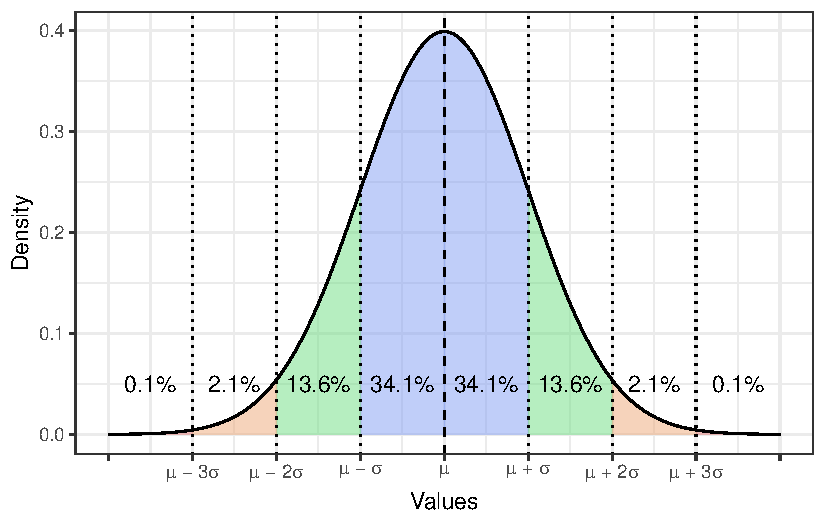
\includegraphics{stats-rand-values_files/figure-pdf/fig-norm-1.pdf}

}

\caption{\label{fig-norm}Нормальное распределение}

\end{figure}%

Задавая различные параметры распределения (математическое ожидание и
дисперсию), мы можем получать разные нормальные распределения
(Рисунок~\ref{fig-norms}).

\begin{figure}

\centering{

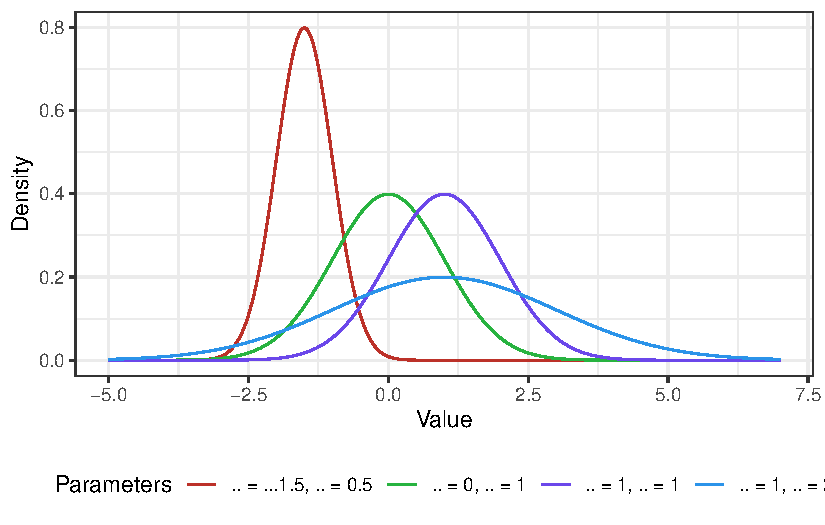
\includegraphics{stats-rand-values_files/figure-pdf/fig-norms-1.pdf}

}

\caption{\label{fig-norms}Нормальное распределение c разными
параметрами}

\end{figure}%

\subsubsection{Стандартное нормальное
распределение}\label{stats-rand-values-stnorm}

\begin{figure}

\centering{

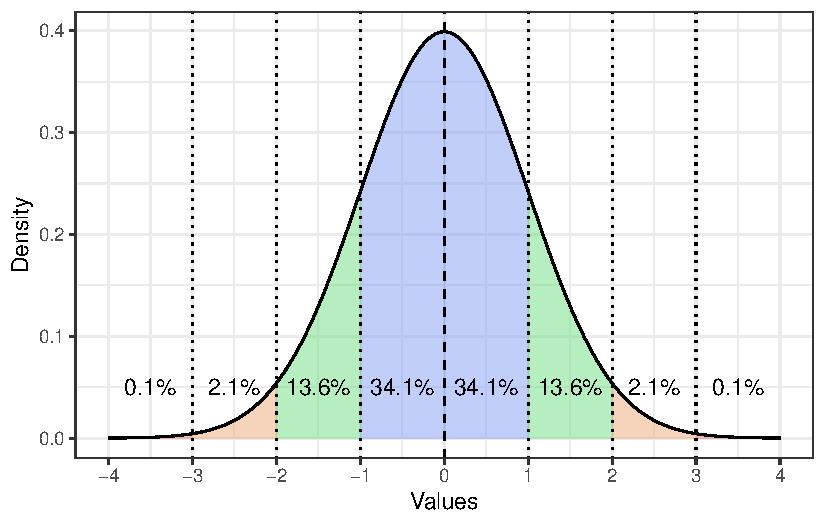
\includegraphics{stats-rand-values_files/figure-pdf/fig-stnorm-1.pdf}

}

\caption{\label{fig-stnorm}Стандартное нормальное распределение}

\end{figure}%

\subsection{Геометрическое распределение}\label{stats-rand-values-geom}

\subsection{Отрицательное биномиальное
распределение}\label{stats-rand-values-negbinom}

\bookmarksetup{startatroot}

\chapter{Оценивание статистических параметров}\label{stats-estim}

Мы оказываемся в сложной, но интересной ситуации. Мы хотим знать что-то
про генеральную совокупность --- значение некоторого \emph{параметра}.
Но мы его никогда не узнаем, потому что не можем работать с целой
генеральной совокупностью. Нам остаётся работать только с
\emph{выборочной совокупность (выборкой)} и опираться на статистические
данные, которые мы собираем на ней.

Выборка извлекается из генеральной совокупности случайным образом,
поэтому что там именно --- с точки зрения данных --- в нашей выборке
будет нам также неизвестно. Отсюда происходят два ключевых свойства
статистических данных --- \emph{неопредлённость} и \emph{вариативность}.

\textbf{Неопределённость} нам говорит о том, что мы не знаем, что именно
мы получим в результате наших измерений для конкретной выборки. В том
числе потому, что мы работаем на просторах случайных величин.

\textbf{Вариативность} означает, что наши данные будут различатся ещё и
от респондента к респонденту. И между выборками тоже. Здесь и ошибка
измерения, и различные смешения и ещё куча всего.

В итоге что мы имеем: так как нам не доступны \emph{истинные} значения
параметров, придётся использовать \emph{оценки} этих параметров.

\section{Точечные
оценки}\label{ux442ux43eux447ux435ux447ux43dux44bux435-ux43eux446ux435ux43dux43aux438}

Параметр обычно обозначается греческой буквой. Пусть у нас есть
некоторый параметр генеральной совокупности \(\theta\). Его аналогом на
выборочной совокупности является его \emph{точечная оценка}
\(\hat \theta\). Точечная она, потому что представляет собой некоторое
одно число. Таким образом, это наиболее компактный способ составить
представление о значении параметра. По своей сути она, на самом деле,
она является функцией от результатов наблюдений:

\[
\hat \theta = \hat \theta (x), \; x = (x_1, x_2, \dots, x_n)
\]

Что это значит? То, что на разных выборках эта оценка может различаться.
Возьмем для примера такой параметр как среднее значение. Предположим,
что мы исследуем интеллект, и наша \emph{генеральная совокупность}
представлена таким набором наблюдений:

\begin{Shaded}
\begin{Highlighting}[]
\FunctionTok{nrow}\NormalTok{(iq)}
\end{Highlighting}
\end{Shaded}

\begin{verbatim}
[1] 10000
\end{verbatim}

\begin{Shaded}
\begin{Highlighting}[]
\FunctionTok{head}\NormalTok{(iq)}
\end{Highlighting}
\end{Shaded}

\begin{verbatim}
# A tibble: 6 x 2
     id    IQ
  <int> <dbl>
1     1    94
2     2   107
3     3    96
4     4    82
5     5   106
6     6    79
\end{verbatim}

\begin{Shaded}
\begin{Highlighting}[]
\FunctionTok{tail}\NormalTok{(iq)}
\end{Highlighting}
\end{Shaded}

\begin{verbatim}
# A tibble: 6 x 2
     id    IQ
  <int> <dbl>
1  9995   112
2  9996   100
3  9997   110
4  9998   110
5  9999    92
6 10000    78
\end{verbatim}

Так как мы предположили, что это генеральная совокупность, то мы можем
посчитать истинное значение параметра \(\mu\). \textbf{В реальной жизни
мы этого сделать не можем!}

\begin{Shaded}
\begin{Highlighting}[]
\FunctionTok{mean}\NormalTok{(iq}\SpecialCharTok{$}\NormalTok{IQ)}
\end{Highlighting}
\end{Shaded}

\begin{verbatim}
[1] 100.0063
\end{verbatim}

Вполне ожидаемое значение\footnote{Шкала IQ устроена так, что её среднее
  значение равно 100, а стандартное отклонение 15.}. Теперь попробуем
наизвлекать выборок человек по 50 и посчитать \emph{оценки среднего
(выборочные средние)} \(\hat \mu\) на них:

\begin{Shaded}
\begin{Highlighting}[]
\NormalTok{means }\OtherTok{\textless{}{-}} \FunctionTok{numeric}\NormalTok{()}
\ControlFlowTok{for}\NormalTok{ (i }\ControlFlowTok{in} \DecValTok{1}\SpecialCharTok{:}\DecValTok{100}\NormalTok{) \{}
\NormalTok{  means[i] }\OtherTok{\textless{}{-}} \FunctionTok{mean}\NormalTok{(}\FunctionTok{sample}\NormalTok{(iq}\SpecialCharTok{$}\NormalTok{IQ, }\DecValTok{50}\NormalTok{, }\AttributeTok{replace =} \ConstantTok{FALSE}\NormalTok{))}
\NormalTok{\}}
\FunctionTok{ggplot}\NormalTok{(}\ConstantTok{NULL}\NormalTok{, }\FunctionTok{aes}\NormalTok{(means)) }\SpecialCharTok{+}
  \FunctionTok{geom\_histogram}\NormalTok{(}\AttributeTok{binwidth =} \DecValTok{1}\NormalTok{, }\AttributeTok{fill =} \StringTok{\textquotesingle{}royalblue4\textquotesingle{}}\NormalTok{, }\AttributeTok{color =} \StringTok{\textquotesingle{}lightgray\textquotesingle{}}\NormalTok{) }\SpecialCharTok{+}
  \FunctionTok{geom\_vline}\NormalTok{(}\AttributeTok{xintercept =} \FunctionTok{mean}\NormalTok{(iq}\SpecialCharTok{$}\NormalTok{IQ)) }\SpecialCharTok{+}
  \FunctionTok{labs}\NormalTok{(}\AttributeTok{x =} \StringTok{\textquotesingle{}Выборочные средние IQ\textquotesingle{}}\NormalTok{,}
       \AttributeTok{y =} \StringTok{\textquotesingle{}Количество\textquotesingle{}}\NormalTok{)}
\end{Highlighting}
\end{Shaded}

\begin{verbatim}
Warning in grid.Call(C_textBounds, as.graphicsAnnot(x$label), x$x, x$y, :
conversion failure on 'Количество' in 'mbcsToSbcs': dot substituted for <d0>
\end{verbatim}

\begin{verbatim}
Warning in grid.Call(C_textBounds, as.graphicsAnnot(x$label), x$x, x$y, :
conversion failure on 'Количество' in 'mbcsToSbcs': dot substituted for <9a>
\end{verbatim}

\begin{verbatim}
Warning in grid.Call(C_textBounds, as.graphicsAnnot(x$label), x$x, x$y, :
conversion failure on 'Количество' in 'mbcsToSbcs': dot substituted for <d0>
\end{verbatim}

\begin{verbatim}
Warning in grid.Call(C_textBounds, as.graphicsAnnot(x$label), x$x, x$y, :
conversion failure on 'Количество' in 'mbcsToSbcs': dot substituted for <be>
\end{verbatim}

\begin{verbatim}
Warning in grid.Call(C_textBounds, as.graphicsAnnot(x$label), x$x, x$y, :
conversion failure on 'Количество' in 'mbcsToSbcs': dot substituted for <d0>
\end{verbatim}

\begin{verbatim}
Warning in grid.Call(C_textBounds, as.graphicsAnnot(x$label), x$x, x$y, :
conversion failure on 'Количество' in 'mbcsToSbcs': dot substituted for <bb>
\end{verbatim}

\begin{verbatim}
Warning in grid.Call(C_textBounds, as.graphicsAnnot(x$label), x$x, x$y, :
conversion failure on 'Количество' in 'mbcsToSbcs': dot substituted for <d0>
\end{verbatim}

\begin{verbatim}
Warning in grid.Call(C_textBounds, as.graphicsAnnot(x$label), x$x, x$y, :
conversion failure on 'Количество' in 'mbcsToSbcs': dot substituted for <b8>
\end{verbatim}

\begin{verbatim}
Warning in grid.Call(C_textBounds, as.graphicsAnnot(x$label), x$x, x$y, :
conversion failure on 'Количество' in 'mbcsToSbcs': dot substituted for <d1>
\end{verbatim}

\begin{verbatim}
Warning in grid.Call(C_textBounds, as.graphicsAnnot(x$label), x$x, x$y, :
conversion failure on 'Количество' in 'mbcsToSbcs': dot substituted for <87>
\end{verbatim}

\begin{verbatim}
Warning in grid.Call(C_textBounds, as.graphicsAnnot(x$label), x$x, x$y, :
conversion failure on 'Количество' in 'mbcsToSbcs': dot substituted for <d0>
\end{verbatim}

\begin{verbatim}
Warning in grid.Call(C_textBounds, as.graphicsAnnot(x$label), x$x, x$y, :
conversion failure on 'Количество' in 'mbcsToSbcs': dot substituted for <b5>
\end{verbatim}

\begin{verbatim}
Warning in grid.Call(C_textBounds, as.graphicsAnnot(x$label), x$x, x$y, :
conversion failure on 'Количество' in 'mbcsToSbcs': dot substituted for <d1>
\end{verbatim}

\begin{verbatim}
Warning in grid.Call(C_textBounds, as.graphicsAnnot(x$label), x$x, x$y, :
conversion failure on 'Количество' in 'mbcsToSbcs': dot substituted for <81>
\end{verbatim}

\begin{verbatim}
Warning in grid.Call(C_textBounds, as.graphicsAnnot(x$label), x$x, x$y, :
conversion failure on 'Количество' in 'mbcsToSbcs': dot substituted for <d1>
\end{verbatim}

\begin{verbatim}
Warning in grid.Call(C_textBounds, as.graphicsAnnot(x$label), x$x, x$y, :
conversion failure on 'Количество' in 'mbcsToSbcs': dot substituted for <82>
\end{verbatim}

\begin{verbatim}
Warning in grid.Call(C_textBounds, as.graphicsAnnot(x$label), x$x, x$y, :
conversion failure on 'Количество' in 'mbcsToSbcs': dot substituted for <d0>
\end{verbatim}

\begin{verbatim}
Warning in grid.Call(C_textBounds, as.graphicsAnnot(x$label), x$x, x$y, :
conversion failure on 'Количество' in 'mbcsToSbcs': dot substituted for <b2>
\end{verbatim}

\begin{verbatim}
Warning in grid.Call(C_textBounds, as.graphicsAnnot(x$label), x$x, x$y, :
conversion failure on 'Количество' in 'mbcsToSbcs': dot substituted for <d0>
\end{verbatim}

\begin{verbatim}
Warning in grid.Call(C_textBounds, as.graphicsAnnot(x$label), x$x, x$y, :
conversion failure on 'Количество' in 'mbcsToSbcs': dot substituted for <be>
\end{verbatim}

\begin{verbatim}
Warning in grid.Call(C_textBounds, as.graphicsAnnot(x$label), x$x, x$y, :
conversion failure on 'Количество' in 'mbcsToSbcs': dot substituted for <d0>
\end{verbatim}

\begin{verbatim}
Warning in grid.Call(C_textBounds, as.graphicsAnnot(x$label), x$x, x$y, :
conversion failure on 'Количество' in 'mbcsToSbcs': dot substituted for <9a>
\end{verbatim}

\begin{verbatim}
Warning in grid.Call(C_textBounds, as.graphicsAnnot(x$label), x$x, x$y, :
conversion failure on 'Количество' in 'mbcsToSbcs': dot substituted for <d0>
\end{verbatim}

\begin{verbatim}
Warning in grid.Call(C_textBounds, as.graphicsAnnot(x$label), x$x, x$y, :
conversion failure on 'Количество' in 'mbcsToSbcs': dot substituted for <be>
\end{verbatim}

\begin{verbatim}
Warning in grid.Call(C_textBounds, as.graphicsAnnot(x$label), x$x, x$y, :
conversion failure on 'Количество' in 'mbcsToSbcs': dot substituted for <d0>
\end{verbatim}

\begin{verbatim}
Warning in grid.Call(C_textBounds, as.graphicsAnnot(x$label), x$x, x$y, :
conversion failure on 'Количество' in 'mbcsToSbcs': dot substituted for <bb>
\end{verbatim}

\begin{verbatim}
Warning in grid.Call(C_textBounds, as.graphicsAnnot(x$label), x$x, x$y, :
conversion failure on 'Количество' in 'mbcsToSbcs': dot substituted for <d0>
\end{verbatim}

\begin{verbatim}
Warning in grid.Call(C_textBounds, as.graphicsAnnot(x$label), x$x, x$y, :
conversion failure on 'Количество' in 'mbcsToSbcs': dot substituted for <b8>
\end{verbatim}

\begin{verbatim}
Warning in grid.Call(C_textBounds, as.graphicsAnnot(x$label), x$x, x$y, :
conversion failure on 'Количество' in 'mbcsToSbcs': dot substituted for <d1>
\end{verbatim}

\begin{verbatim}
Warning in grid.Call(C_textBounds, as.graphicsAnnot(x$label), x$x, x$y, :
conversion failure on 'Количество' in 'mbcsToSbcs': dot substituted for <87>
\end{verbatim}

\begin{verbatim}
Warning in grid.Call(C_textBounds, as.graphicsAnnot(x$label), x$x, x$y, :
conversion failure on 'Количество' in 'mbcsToSbcs': dot substituted for <d0>
\end{verbatim}

\begin{verbatim}
Warning in grid.Call(C_textBounds, as.graphicsAnnot(x$label), x$x, x$y, :
conversion failure on 'Количество' in 'mbcsToSbcs': dot substituted for <b5>
\end{verbatim}

\begin{verbatim}
Warning in grid.Call(C_textBounds, as.graphicsAnnot(x$label), x$x, x$y, :
conversion failure on 'Количество' in 'mbcsToSbcs': dot substituted for <d1>
\end{verbatim}

\begin{verbatim}
Warning in grid.Call(C_textBounds, as.graphicsAnnot(x$label), x$x, x$y, :
conversion failure on 'Количество' in 'mbcsToSbcs': dot substituted for <81>
\end{verbatim}

\begin{verbatim}
Warning in grid.Call(C_textBounds, as.graphicsAnnot(x$label), x$x, x$y, :
conversion failure on 'Количество' in 'mbcsToSbcs': dot substituted for <d1>
\end{verbatim}

\begin{verbatim}
Warning in grid.Call(C_textBounds, as.graphicsAnnot(x$label), x$x, x$y, :
conversion failure on 'Количество' in 'mbcsToSbcs': dot substituted for <82>
\end{verbatim}

\begin{verbatim}
Warning in grid.Call(C_textBounds, as.graphicsAnnot(x$label), x$x, x$y, :
conversion failure on 'Количество' in 'mbcsToSbcs': dot substituted for <d0>
\end{verbatim}

\begin{verbatim}
Warning in grid.Call(C_textBounds, as.graphicsAnnot(x$label), x$x, x$y, :
conversion failure on 'Количество' in 'mbcsToSbcs': dot substituted for <b2>
\end{verbatim}

\begin{verbatim}
Warning in grid.Call(C_textBounds, as.graphicsAnnot(x$label), x$x, x$y, :
conversion failure on 'Количество' in 'mbcsToSbcs': dot substituted for <d0>
\end{verbatim}

\begin{verbatim}
Warning in grid.Call(C_textBounds, as.graphicsAnnot(x$label), x$x, x$y, :
conversion failure on 'Количество' in 'mbcsToSbcs': dot substituted for <be>
\end{verbatim}

\begin{verbatim}
Warning in grid.Call(C_textBounds, as.graphicsAnnot(x$label), x$x, x$y, :
conversion failure on 'Выборочные средние IQ' in 'mbcsToSbcs': dot substituted
for <d0>
\end{verbatim}

\begin{verbatim}
Warning in grid.Call(C_textBounds, as.graphicsAnnot(x$label), x$x, x$y, :
conversion failure on 'Выборочные средние IQ' in 'mbcsToSbcs': dot substituted
for <92>
\end{verbatim}

\begin{verbatim}
Warning in grid.Call(C_textBounds, as.graphicsAnnot(x$label), x$x, x$y, :
conversion failure on 'Выборочные средние IQ' in 'mbcsToSbcs': dot substituted
for <d1>
\end{verbatim}

\begin{verbatim}
Warning in grid.Call(C_textBounds, as.graphicsAnnot(x$label), x$x, x$y, :
conversion failure on 'Выборочные средние IQ' in 'mbcsToSbcs': dot substituted
for <8b>
\end{verbatim}

\begin{verbatim}
Warning in grid.Call(C_textBounds, as.graphicsAnnot(x$label), x$x, x$y, :
conversion failure on 'Выборочные средние IQ' in 'mbcsToSbcs': dot substituted
for <d0>
\end{verbatim}

\begin{verbatim}
Warning in grid.Call(C_textBounds, as.graphicsAnnot(x$label), x$x, x$y, :
conversion failure on 'Выборочные средние IQ' in 'mbcsToSbcs': dot substituted
for <b1>
\end{verbatim}

\begin{verbatim}
Warning in grid.Call(C_textBounds, as.graphicsAnnot(x$label), x$x, x$y, :
conversion failure on 'Выборочные средние IQ' in 'mbcsToSbcs': dot substituted
for <d0>
\end{verbatim}

\begin{verbatim}
Warning in grid.Call(C_textBounds, as.graphicsAnnot(x$label), x$x, x$y, :
conversion failure on 'Выборочные средние IQ' in 'mbcsToSbcs': dot substituted
for <be>
\end{verbatim}

\begin{verbatim}
Warning in grid.Call(C_textBounds, as.graphicsAnnot(x$label), x$x, x$y, :
conversion failure on 'Выборочные средние IQ' in 'mbcsToSbcs': dot substituted
for <d1>
\end{verbatim}

\begin{verbatim}
Warning in grid.Call(C_textBounds, as.graphicsAnnot(x$label), x$x, x$y, :
conversion failure on 'Выборочные средние IQ' in 'mbcsToSbcs': dot substituted
for <80>
\end{verbatim}

\begin{verbatim}
Warning in grid.Call(C_textBounds, as.graphicsAnnot(x$label), x$x, x$y, :
conversion failure on 'Выборочные средние IQ' in 'mbcsToSbcs': dot substituted
for <d0>
\end{verbatim}

\begin{verbatim}
Warning in grid.Call(C_textBounds, as.graphicsAnnot(x$label), x$x, x$y, :
conversion failure on 'Выборочные средние IQ' in 'mbcsToSbcs': dot substituted
for <be>
\end{verbatim}

\begin{verbatim}
Warning in grid.Call(C_textBounds, as.graphicsAnnot(x$label), x$x, x$y, :
conversion failure on 'Выборочные средние IQ' in 'mbcsToSbcs': dot substituted
for <d1>
\end{verbatim}

\begin{verbatim}
Warning in grid.Call(C_textBounds, as.graphicsAnnot(x$label), x$x, x$y, :
conversion failure on 'Выборочные средние IQ' in 'mbcsToSbcs': dot substituted
for <87>
\end{verbatim}

\begin{verbatim}
Warning in grid.Call(C_textBounds, as.graphicsAnnot(x$label), x$x, x$y, :
conversion failure on 'Выборочные средние IQ' in 'mbcsToSbcs': dot substituted
for <d0>
\end{verbatim}

\begin{verbatim}
Warning in grid.Call(C_textBounds, as.graphicsAnnot(x$label), x$x, x$y, :
conversion failure on 'Выборочные средние IQ' in 'mbcsToSbcs': dot substituted
for <bd>
\end{verbatim}

\begin{verbatim}
Warning in grid.Call(C_textBounds, as.graphicsAnnot(x$label), x$x, x$y, :
conversion failure on 'Выборочные средние IQ' in 'mbcsToSbcs': dot substituted
for <d1>
\end{verbatim}

\begin{verbatim}
Warning in grid.Call(C_textBounds, as.graphicsAnnot(x$label), x$x, x$y, :
conversion failure on 'Выборочные средние IQ' in 'mbcsToSbcs': dot substituted
for <8b>
\end{verbatim}

\begin{verbatim}
Warning in grid.Call(C_textBounds, as.graphicsAnnot(x$label), x$x, x$y, :
conversion failure on 'Выборочные средние IQ' in 'mbcsToSbcs': dot substituted
for <d0>
\end{verbatim}

\begin{verbatim}
Warning in grid.Call(C_textBounds, as.graphicsAnnot(x$label), x$x, x$y, :
conversion failure on 'Выборочные средние IQ' in 'mbcsToSbcs': dot substituted
for <b5>
\end{verbatim}

\begin{verbatim}
Warning in grid.Call(C_textBounds, as.graphicsAnnot(x$label), x$x, x$y, :
conversion failure on 'Выборочные средние IQ' in 'mbcsToSbcs': dot substituted
for <d1>
\end{verbatim}

\begin{verbatim}
Warning in grid.Call(C_textBounds, as.graphicsAnnot(x$label), x$x, x$y, :
conversion failure on 'Выборочные средние IQ' in 'mbcsToSbcs': dot substituted
for <81>
\end{verbatim}

\begin{verbatim}
Warning in grid.Call(C_textBounds, as.graphicsAnnot(x$label), x$x, x$y, :
conversion failure on 'Выборочные средние IQ' in 'mbcsToSbcs': dot substituted
for <d1>
\end{verbatim}

\begin{verbatim}
Warning in grid.Call(C_textBounds, as.graphicsAnnot(x$label), x$x, x$y, :
conversion failure on 'Выборочные средние IQ' in 'mbcsToSbcs': dot substituted
for <80>
\end{verbatim}

\begin{verbatim}
Warning in grid.Call(C_textBounds, as.graphicsAnnot(x$label), x$x, x$y, :
conversion failure on 'Выборочные средние IQ' in 'mbcsToSbcs': dot substituted
for <d0>
\end{verbatim}

\begin{verbatim}
Warning in grid.Call(C_textBounds, as.graphicsAnnot(x$label), x$x, x$y, :
conversion failure on 'Выборочные средние IQ' in 'mbcsToSbcs': dot substituted
for <b5>
\end{verbatim}

\begin{verbatim}
Warning in grid.Call(C_textBounds, as.graphicsAnnot(x$label), x$x, x$y, :
conversion failure on 'Выборочные средние IQ' in 'mbcsToSbcs': dot substituted
for <d0>
\end{verbatim}

\begin{verbatim}
Warning in grid.Call(C_textBounds, as.graphicsAnnot(x$label), x$x, x$y, :
conversion failure on 'Выборочные средние IQ' in 'mbcsToSbcs': dot substituted
for <b4>
\end{verbatim}

\begin{verbatim}
Warning in grid.Call(C_textBounds, as.graphicsAnnot(x$label), x$x, x$y, :
conversion failure on 'Выборочные средние IQ' in 'mbcsToSbcs': dot substituted
for <d0>
\end{verbatim}

\begin{verbatim}
Warning in grid.Call(C_textBounds, as.graphicsAnnot(x$label), x$x, x$y, :
conversion failure on 'Выборочные средние IQ' in 'mbcsToSbcs': dot substituted
for <bd>
\end{verbatim}

\begin{verbatim}
Warning in grid.Call(C_textBounds, as.graphicsAnnot(x$label), x$x, x$y, :
conversion failure on 'Выборочные средние IQ' in 'mbcsToSbcs': dot substituted
for <d0>
\end{verbatim}

\begin{verbatim}
Warning in grid.Call(C_textBounds, as.graphicsAnnot(x$label), x$x, x$y, :
conversion failure on 'Выборочные средние IQ' in 'mbcsToSbcs': dot substituted
for <b8>
\end{verbatim}

\begin{verbatim}
Warning in grid.Call(C_textBounds, as.graphicsAnnot(x$label), x$x, x$y, :
conversion failure on 'Выборочные средние IQ' in 'mbcsToSbcs': dot substituted
for <d0>
\end{verbatim}

\begin{verbatim}
Warning in grid.Call(C_textBounds, as.graphicsAnnot(x$label), x$x, x$y, :
conversion failure on 'Выборочные средние IQ' in 'mbcsToSbcs': dot substituted
for <b5>
\end{verbatim}

\begin{verbatim}
Warning in grid.Call(C_textBounds, as.graphicsAnnot(x$label), x$x, x$y, :
conversion failure on 'Выборочные средние IQ' in 'mbcsToSbcs': dot substituted
for <d0>
\end{verbatim}

\begin{verbatim}
Warning in grid.Call(C_textBounds, as.graphicsAnnot(x$label), x$x, x$y, :
conversion failure on 'Выборочные средние IQ' in 'mbcsToSbcs': dot substituted
for <92>
\end{verbatim}

\begin{verbatim}
Warning in grid.Call(C_textBounds, as.graphicsAnnot(x$label), x$x, x$y, :
conversion failure on 'Выборочные средние IQ' in 'mbcsToSbcs': dot substituted
for <d1>
\end{verbatim}

\begin{verbatim}
Warning in grid.Call(C_textBounds, as.graphicsAnnot(x$label), x$x, x$y, :
conversion failure on 'Выборочные средние IQ' in 'mbcsToSbcs': dot substituted
for <8b>
\end{verbatim}

\begin{verbatim}
Warning in grid.Call(C_textBounds, as.graphicsAnnot(x$label), x$x, x$y, :
conversion failure on 'Выборочные средние IQ' in 'mbcsToSbcs': dot substituted
for <d0>
\end{verbatim}

\begin{verbatim}
Warning in grid.Call(C_textBounds, as.graphicsAnnot(x$label), x$x, x$y, :
conversion failure on 'Выборочные средние IQ' in 'mbcsToSbcs': dot substituted
for <b1>
\end{verbatim}

\begin{verbatim}
Warning in grid.Call(C_textBounds, as.graphicsAnnot(x$label), x$x, x$y, :
conversion failure on 'Выборочные средние IQ' in 'mbcsToSbcs': dot substituted
for <d0>
\end{verbatim}

\begin{verbatim}
Warning in grid.Call(C_textBounds, as.graphicsAnnot(x$label), x$x, x$y, :
conversion failure on 'Выборочные средние IQ' in 'mbcsToSbcs': dot substituted
for <be>
\end{verbatim}

\begin{verbatim}
Warning in grid.Call(C_textBounds, as.graphicsAnnot(x$label), x$x, x$y, :
conversion failure on 'Выборочные средние IQ' in 'mbcsToSbcs': dot substituted
for <d1>
\end{verbatim}

\begin{verbatim}
Warning in grid.Call(C_textBounds, as.graphicsAnnot(x$label), x$x, x$y, :
conversion failure on 'Выборочные средние IQ' in 'mbcsToSbcs': dot substituted
for <80>
\end{verbatim}

\begin{verbatim}
Warning in grid.Call(C_textBounds, as.graphicsAnnot(x$label), x$x, x$y, :
conversion failure on 'Выборочные средние IQ' in 'mbcsToSbcs': dot substituted
for <d0>
\end{verbatim}

\begin{verbatim}
Warning in grid.Call(C_textBounds, as.graphicsAnnot(x$label), x$x, x$y, :
conversion failure on 'Выборочные средние IQ' in 'mbcsToSbcs': dot substituted
for <be>
\end{verbatim}

\begin{verbatim}
Warning in grid.Call(C_textBounds, as.graphicsAnnot(x$label), x$x, x$y, :
conversion failure on 'Выборочные средние IQ' in 'mbcsToSbcs': dot substituted
for <d1>
\end{verbatim}

\begin{verbatim}
Warning in grid.Call(C_textBounds, as.graphicsAnnot(x$label), x$x, x$y, :
conversion failure on 'Выборочные средние IQ' in 'mbcsToSbcs': dot substituted
for <87>
\end{verbatim}

\begin{verbatim}
Warning in grid.Call(C_textBounds, as.graphicsAnnot(x$label), x$x, x$y, :
conversion failure on 'Выборочные средние IQ' in 'mbcsToSbcs': dot substituted
for <d0>
\end{verbatim}

\begin{verbatim}
Warning in grid.Call(C_textBounds, as.graphicsAnnot(x$label), x$x, x$y, :
conversion failure on 'Выборочные средние IQ' in 'mbcsToSbcs': dot substituted
for <bd>
\end{verbatim}

\begin{verbatim}
Warning in grid.Call(C_textBounds, as.graphicsAnnot(x$label), x$x, x$y, :
conversion failure on 'Выборочные средние IQ' in 'mbcsToSbcs': dot substituted
for <d1>
\end{verbatim}

\begin{verbatim}
Warning in grid.Call(C_textBounds, as.graphicsAnnot(x$label), x$x, x$y, :
conversion failure on 'Выборочные средние IQ' in 'mbcsToSbcs': dot substituted
for <8b>
\end{verbatim}

\begin{verbatim}
Warning in grid.Call(C_textBounds, as.graphicsAnnot(x$label), x$x, x$y, :
conversion failure on 'Выборочные средние IQ' in 'mbcsToSbcs': dot substituted
for <d0>
\end{verbatim}

\begin{verbatim}
Warning in grid.Call(C_textBounds, as.graphicsAnnot(x$label), x$x, x$y, :
conversion failure on 'Выборочные средние IQ' in 'mbcsToSbcs': dot substituted
for <b5>
\end{verbatim}

\begin{verbatim}
Warning in grid.Call(C_textBounds, as.graphicsAnnot(x$label), x$x, x$y, :
conversion failure on 'Выборочные средние IQ' in 'mbcsToSbcs': dot substituted
for <d1>
\end{verbatim}

\begin{verbatim}
Warning in grid.Call(C_textBounds, as.graphicsAnnot(x$label), x$x, x$y, :
conversion failure on 'Выборочные средние IQ' in 'mbcsToSbcs': dot substituted
for <81>
\end{verbatim}

\begin{verbatim}
Warning in grid.Call(C_textBounds, as.graphicsAnnot(x$label), x$x, x$y, :
conversion failure on 'Выборочные средние IQ' in 'mbcsToSbcs': dot substituted
for <d1>
\end{verbatim}

\begin{verbatim}
Warning in grid.Call(C_textBounds, as.graphicsAnnot(x$label), x$x, x$y, :
conversion failure on 'Выборочные средние IQ' in 'mbcsToSbcs': dot substituted
for <80>
\end{verbatim}

\begin{verbatim}
Warning in grid.Call(C_textBounds, as.graphicsAnnot(x$label), x$x, x$y, :
conversion failure on 'Выборочные средние IQ' in 'mbcsToSbcs': dot substituted
for <d0>
\end{verbatim}

\begin{verbatim}
Warning in grid.Call(C_textBounds, as.graphicsAnnot(x$label), x$x, x$y, :
conversion failure on 'Выборочные средние IQ' in 'mbcsToSbcs': dot substituted
for <b5>
\end{verbatim}

\begin{verbatim}
Warning in grid.Call(C_textBounds, as.graphicsAnnot(x$label), x$x, x$y, :
conversion failure on 'Выборочные средние IQ' in 'mbcsToSbcs': dot substituted
for <d0>
\end{verbatim}

\begin{verbatim}
Warning in grid.Call(C_textBounds, as.graphicsAnnot(x$label), x$x, x$y, :
conversion failure on 'Выборочные средние IQ' in 'mbcsToSbcs': dot substituted
for <b4>
\end{verbatim}

\begin{verbatim}
Warning in grid.Call(C_textBounds, as.graphicsAnnot(x$label), x$x, x$y, :
conversion failure on 'Выборочные средние IQ' in 'mbcsToSbcs': dot substituted
for <d0>
\end{verbatim}

\begin{verbatim}
Warning in grid.Call(C_textBounds, as.graphicsAnnot(x$label), x$x, x$y, :
conversion failure on 'Выборочные средние IQ' in 'mbcsToSbcs': dot substituted
for <bd>
\end{verbatim}

\begin{verbatim}
Warning in grid.Call(C_textBounds, as.graphicsAnnot(x$label), x$x, x$y, :
conversion failure on 'Выборочные средние IQ' in 'mbcsToSbcs': dot substituted
for <d0>
\end{verbatim}

\begin{verbatim}
Warning in grid.Call(C_textBounds, as.graphicsAnnot(x$label), x$x, x$y, :
conversion failure on 'Выборочные средние IQ' in 'mbcsToSbcs': dot substituted
for <b8>
\end{verbatim}

\begin{verbatim}
Warning in grid.Call(C_textBounds, as.graphicsAnnot(x$label), x$x, x$y, :
conversion failure on 'Выборочные средние IQ' in 'mbcsToSbcs': dot substituted
for <d0>
\end{verbatim}

\begin{verbatim}
Warning in grid.Call(C_textBounds, as.graphicsAnnot(x$label), x$x, x$y, :
conversion failure on 'Выборочные средние IQ' in 'mbcsToSbcs': dot substituted
for <b5>
\end{verbatim}

\begin{verbatim}
Warning in grid.Call(C_textBounds, as.graphicsAnnot(x$label), x$x, x$y, :
conversion failure on 'Количество' in 'mbcsToSbcs': dot substituted for <d0>
\end{verbatim}

\begin{verbatim}
Warning in grid.Call(C_textBounds, as.graphicsAnnot(x$label), x$x, x$y, :
conversion failure on 'Количество' in 'mbcsToSbcs': dot substituted for <9a>
\end{verbatim}

\begin{verbatim}
Warning in grid.Call(C_textBounds, as.graphicsAnnot(x$label), x$x, x$y, :
conversion failure on 'Количество' in 'mbcsToSbcs': dot substituted for <d0>
\end{verbatim}

\begin{verbatim}
Warning in grid.Call(C_textBounds, as.graphicsAnnot(x$label), x$x, x$y, :
conversion failure on 'Количество' in 'mbcsToSbcs': dot substituted for <be>
\end{verbatim}

\begin{verbatim}
Warning in grid.Call(C_textBounds, as.graphicsAnnot(x$label), x$x, x$y, :
conversion failure on 'Количество' in 'mbcsToSbcs': dot substituted for <d0>
\end{verbatim}

\begin{verbatim}
Warning in grid.Call(C_textBounds, as.graphicsAnnot(x$label), x$x, x$y, :
conversion failure on 'Количество' in 'mbcsToSbcs': dot substituted for <bb>
\end{verbatim}

\begin{verbatim}
Warning in grid.Call(C_textBounds, as.graphicsAnnot(x$label), x$x, x$y, :
conversion failure on 'Количество' in 'mbcsToSbcs': dot substituted for <d0>
\end{verbatim}

\begin{verbatim}
Warning in grid.Call(C_textBounds, as.graphicsAnnot(x$label), x$x, x$y, :
conversion failure on 'Количество' in 'mbcsToSbcs': dot substituted for <b8>
\end{verbatim}

\begin{verbatim}
Warning in grid.Call(C_textBounds, as.graphicsAnnot(x$label), x$x, x$y, :
conversion failure on 'Количество' in 'mbcsToSbcs': dot substituted for <d1>
\end{verbatim}

\begin{verbatim}
Warning in grid.Call(C_textBounds, as.graphicsAnnot(x$label), x$x, x$y, :
conversion failure on 'Количество' in 'mbcsToSbcs': dot substituted for <87>
\end{verbatim}

\begin{verbatim}
Warning in grid.Call(C_textBounds, as.graphicsAnnot(x$label), x$x, x$y, :
conversion failure on 'Количество' in 'mbcsToSbcs': dot substituted for <d0>
\end{verbatim}

\begin{verbatim}
Warning in grid.Call(C_textBounds, as.graphicsAnnot(x$label), x$x, x$y, :
conversion failure on 'Количество' in 'mbcsToSbcs': dot substituted for <b5>
\end{verbatim}

\begin{verbatim}
Warning in grid.Call(C_textBounds, as.graphicsAnnot(x$label), x$x, x$y, :
conversion failure on 'Количество' in 'mbcsToSbcs': dot substituted for <d1>
\end{verbatim}

\begin{verbatim}
Warning in grid.Call(C_textBounds, as.graphicsAnnot(x$label), x$x, x$y, :
conversion failure on 'Количество' in 'mbcsToSbcs': dot substituted for <81>
\end{verbatim}

\begin{verbatim}
Warning in grid.Call(C_textBounds, as.graphicsAnnot(x$label), x$x, x$y, :
conversion failure on 'Количество' in 'mbcsToSbcs': dot substituted for <d1>
\end{verbatim}

\begin{verbatim}
Warning in grid.Call(C_textBounds, as.graphicsAnnot(x$label), x$x, x$y, :
conversion failure on 'Количество' in 'mbcsToSbcs': dot substituted for <82>
\end{verbatim}

\begin{verbatim}
Warning in grid.Call(C_textBounds, as.graphicsAnnot(x$label), x$x, x$y, :
conversion failure on 'Количество' in 'mbcsToSbcs': dot substituted for <d0>
\end{verbatim}

\begin{verbatim}
Warning in grid.Call(C_textBounds, as.graphicsAnnot(x$label), x$x, x$y, :
conversion failure on 'Количество' in 'mbcsToSbcs': dot substituted for <b2>
\end{verbatim}

\begin{verbatim}
Warning in grid.Call(C_textBounds, as.graphicsAnnot(x$label), x$x, x$y, :
conversion failure on 'Количество' in 'mbcsToSbcs': dot substituted for <d0>
\end{verbatim}

\begin{verbatim}
Warning in grid.Call(C_textBounds, as.graphicsAnnot(x$label), x$x, x$y, :
conversion failure on 'Количество' in 'mbcsToSbcs': dot substituted for <be>
\end{verbatim}

\begin{verbatim}
Warning in grid.Call(C_textBounds, as.graphicsAnnot(x$label), x$x, x$y, :
conversion failure on 'Количество' in 'mbcsToSbcs': dot substituted for <d0>
\end{verbatim}

\begin{verbatim}
Warning in grid.Call(C_textBounds, as.graphicsAnnot(x$label), x$x, x$y, :
conversion failure on 'Количество' in 'mbcsToSbcs': dot substituted for <9a>
\end{verbatim}

\begin{verbatim}
Warning in grid.Call(C_textBounds, as.graphicsAnnot(x$label), x$x, x$y, :
conversion failure on 'Количество' in 'mbcsToSbcs': dot substituted for <d0>
\end{verbatim}

\begin{verbatim}
Warning in grid.Call(C_textBounds, as.graphicsAnnot(x$label), x$x, x$y, :
conversion failure on 'Количество' in 'mbcsToSbcs': dot substituted for <be>
\end{verbatim}

\begin{verbatim}
Warning in grid.Call(C_textBounds, as.graphicsAnnot(x$label), x$x, x$y, :
conversion failure on 'Количество' in 'mbcsToSbcs': dot substituted for <d0>
\end{verbatim}

\begin{verbatim}
Warning in grid.Call(C_textBounds, as.graphicsAnnot(x$label), x$x, x$y, :
conversion failure on 'Количество' in 'mbcsToSbcs': dot substituted for <bb>
\end{verbatim}

\begin{verbatim}
Warning in grid.Call(C_textBounds, as.graphicsAnnot(x$label), x$x, x$y, :
conversion failure on 'Количество' in 'mbcsToSbcs': dot substituted for <d0>
\end{verbatim}

\begin{verbatim}
Warning in grid.Call(C_textBounds, as.graphicsAnnot(x$label), x$x, x$y, :
conversion failure on 'Количество' in 'mbcsToSbcs': dot substituted for <b8>
\end{verbatim}

\begin{verbatim}
Warning in grid.Call(C_textBounds, as.graphicsAnnot(x$label), x$x, x$y, :
conversion failure on 'Количество' in 'mbcsToSbcs': dot substituted for <d1>
\end{verbatim}

\begin{verbatim}
Warning in grid.Call(C_textBounds, as.graphicsAnnot(x$label), x$x, x$y, :
conversion failure on 'Количество' in 'mbcsToSbcs': dot substituted for <87>
\end{verbatim}

\begin{verbatim}
Warning in grid.Call(C_textBounds, as.graphicsAnnot(x$label), x$x, x$y, :
conversion failure on 'Количество' in 'mbcsToSbcs': dot substituted for <d0>
\end{verbatim}

\begin{verbatim}
Warning in grid.Call(C_textBounds, as.graphicsAnnot(x$label), x$x, x$y, :
conversion failure on 'Количество' in 'mbcsToSbcs': dot substituted for <b5>
\end{verbatim}

\begin{verbatim}
Warning in grid.Call(C_textBounds, as.graphicsAnnot(x$label), x$x, x$y, :
conversion failure on 'Количество' in 'mbcsToSbcs': dot substituted for <d1>
\end{verbatim}

\begin{verbatim}
Warning in grid.Call(C_textBounds, as.graphicsAnnot(x$label), x$x, x$y, :
conversion failure on 'Количество' in 'mbcsToSbcs': dot substituted for <81>
\end{verbatim}

\begin{verbatim}
Warning in grid.Call(C_textBounds, as.graphicsAnnot(x$label), x$x, x$y, :
conversion failure on 'Количество' in 'mbcsToSbcs': dot substituted for <d1>
\end{verbatim}

\begin{verbatim}
Warning in grid.Call(C_textBounds, as.graphicsAnnot(x$label), x$x, x$y, :
conversion failure on 'Количество' in 'mbcsToSbcs': dot substituted for <82>
\end{verbatim}

\begin{verbatim}
Warning in grid.Call(C_textBounds, as.graphicsAnnot(x$label), x$x, x$y, :
conversion failure on 'Количество' in 'mbcsToSbcs': dot substituted for <d0>
\end{verbatim}

\begin{verbatim}
Warning in grid.Call(C_textBounds, as.graphicsAnnot(x$label), x$x, x$y, :
conversion failure on 'Количество' in 'mbcsToSbcs': dot substituted for <b2>
\end{verbatim}

\begin{verbatim}
Warning in grid.Call(C_textBounds, as.graphicsAnnot(x$label), x$x, x$y, :
conversion failure on 'Количество' in 'mbcsToSbcs': dot substituted for <d0>
\end{verbatim}

\begin{verbatim}
Warning in grid.Call(C_textBounds, as.graphicsAnnot(x$label), x$x, x$y, :
conversion failure on 'Количество' in 'mbcsToSbcs': dot substituted for <be>
\end{verbatim}

\begin{verbatim}
Warning in grid.Call(C_textBounds, as.graphicsAnnot(x$label), x$x, x$y, :
conversion failure on 'Количество' in 'mbcsToSbcs': dot substituted for <d0>
\end{verbatim}

\begin{verbatim}
Warning in grid.Call(C_textBounds, as.graphicsAnnot(x$label), x$x, x$y, :
conversion failure on 'Количество' in 'mbcsToSbcs': dot substituted for <9a>
\end{verbatim}

\begin{verbatim}
Warning in grid.Call(C_textBounds, as.graphicsAnnot(x$label), x$x, x$y, :
conversion failure on 'Количество' in 'mbcsToSbcs': dot substituted for <d0>
\end{verbatim}

\begin{verbatim}
Warning in grid.Call(C_textBounds, as.graphicsAnnot(x$label), x$x, x$y, :
conversion failure on 'Количество' in 'mbcsToSbcs': dot substituted for <be>
\end{verbatim}

\begin{verbatim}
Warning in grid.Call(C_textBounds, as.graphicsAnnot(x$label), x$x, x$y, :
conversion failure on 'Количество' in 'mbcsToSbcs': dot substituted for <d0>
\end{verbatim}

\begin{verbatim}
Warning in grid.Call(C_textBounds, as.graphicsAnnot(x$label), x$x, x$y, :
conversion failure on 'Количество' in 'mbcsToSbcs': dot substituted for <bb>
\end{verbatim}

\begin{verbatim}
Warning in grid.Call(C_textBounds, as.graphicsAnnot(x$label), x$x, x$y, :
conversion failure on 'Количество' in 'mbcsToSbcs': dot substituted for <d0>
\end{verbatim}

\begin{verbatim}
Warning in grid.Call(C_textBounds, as.graphicsAnnot(x$label), x$x, x$y, :
conversion failure on 'Количество' in 'mbcsToSbcs': dot substituted for <b8>
\end{verbatim}

\begin{verbatim}
Warning in grid.Call(C_textBounds, as.graphicsAnnot(x$label), x$x, x$y, :
conversion failure on 'Количество' in 'mbcsToSbcs': dot substituted for <d1>
\end{verbatim}

\begin{verbatim}
Warning in grid.Call(C_textBounds, as.graphicsAnnot(x$label), x$x, x$y, :
conversion failure on 'Количество' in 'mbcsToSbcs': dot substituted for <87>
\end{verbatim}

\begin{verbatim}
Warning in grid.Call(C_textBounds, as.graphicsAnnot(x$label), x$x, x$y, :
conversion failure on 'Количество' in 'mbcsToSbcs': dot substituted for <d0>
\end{verbatim}

\begin{verbatim}
Warning in grid.Call(C_textBounds, as.graphicsAnnot(x$label), x$x, x$y, :
conversion failure on 'Количество' in 'mbcsToSbcs': dot substituted for <b5>
\end{verbatim}

\begin{verbatim}
Warning in grid.Call(C_textBounds, as.graphicsAnnot(x$label), x$x, x$y, :
conversion failure on 'Количество' in 'mbcsToSbcs': dot substituted for <d1>
\end{verbatim}

\begin{verbatim}
Warning in grid.Call(C_textBounds, as.graphicsAnnot(x$label), x$x, x$y, :
conversion failure on 'Количество' in 'mbcsToSbcs': dot substituted for <81>
\end{verbatim}

\begin{verbatim}
Warning in grid.Call(C_textBounds, as.graphicsAnnot(x$label), x$x, x$y, :
conversion failure on 'Количество' in 'mbcsToSbcs': dot substituted for <d1>
\end{verbatim}

\begin{verbatim}
Warning in grid.Call(C_textBounds, as.graphicsAnnot(x$label), x$x, x$y, :
conversion failure on 'Количество' in 'mbcsToSbcs': dot substituted for <82>
\end{verbatim}

\begin{verbatim}
Warning in grid.Call(C_textBounds, as.graphicsAnnot(x$label), x$x, x$y, :
conversion failure on 'Количество' in 'mbcsToSbcs': dot substituted for <d0>
\end{verbatim}

\begin{verbatim}
Warning in grid.Call(C_textBounds, as.graphicsAnnot(x$label), x$x, x$y, :
conversion failure on 'Количество' in 'mbcsToSbcs': dot substituted for <b2>
\end{verbatim}

\begin{verbatim}
Warning in grid.Call(C_textBounds, as.graphicsAnnot(x$label), x$x, x$y, :
conversion failure on 'Количество' in 'mbcsToSbcs': dot substituted for <d0>
\end{verbatim}

\begin{verbatim}
Warning in grid.Call(C_textBounds, as.graphicsAnnot(x$label), x$x, x$y, :
conversion failure on 'Количество' in 'mbcsToSbcs': dot substituted for <be>
\end{verbatim}

\begin{verbatim}
Warning in grid.Call(C_textBounds, as.graphicsAnnot(x$label), x$x, x$y, :
conversion failure on 'Выборочные средние IQ' in 'mbcsToSbcs': dot substituted
for <d0>
\end{verbatim}

\begin{verbatim}
Warning in grid.Call(C_textBounds, as.graphicsAnnot(x$label), x$x, x$y, :
conversion failure on 'Выборочные средние IQ' in 'mbcsToSbcs': dot substituted
for <92>
\end{verbatim}

\begin{verbatim}
Warning in grid.Call(C_textBounds, as.graphicsAnnot(x$label), x$x, x$y, :
conversion failure on 'Выборочные средние IQ' in 'mbcsToSbcs': dot substituted
for <d1>
\end{verbatim}

\begin{verbatim}
Warning in grid.Call(C_textBounds, as.graphicsAnnot(x$label), x$x, x$y, :
conversion failure on 'Выборочные средние IQ' in 'mbcsToSbcs': dot substituted
for <8b>
\end{verbatim}

\begin{verbatim}
Warning in grid.Call(C_textBounds, as.graphicsAnnot(x$label), x$x, x$y, :
conversion failure on 'Выборочные средние IQ' in 'mbcsToSbcs': dot substituted
for <d0>
\end{verbatim}

\begin{verbatim}
Warning in grid.Call(C_textBounds, as.graphicsAnnot(x$label), x$x, x$y, :
conversion failure on 'Выборочные средние IQ' in 'mbcsToSbcs': dot substituted
for <b1>
\end{verbatim}

\begin{verbatim}
Warning in grid.Call(C_textBounds, as.graphicsAnnot(x$label), x$x, x$y, :
conversion failure on 'Выборочные средние IQ' in 'mbcsToSbcs': dot substituted
for <d0>
\end{verbatim}

\begin{verbatim}
Warning in grid.Call(C_textBounds, as.graphicsAnnot(x$label), x$x, x$y, :
conversion failure on 'Выборочные средние IQ' in 'mbcsToSbcs': dot substituted
for <be>
\end{verbatim}

\begin{verbatim}
Warning in grid.Call(C_textBounds, as.graphicsAnnot(x$label), x$x, x$y, :
conversion failure on 'Выборочные средние IQ' in 'mbcsToSbcs': dot substituted
for <d1>
\end{verbatim}

\begin{verbatim}
Warning in grid.Call(C_textBounds, as.graphicsAnnot(x$label), x$x, x$y, :
conversion failure on 'Выборочные средние IQ' in 'mbcsToSbcs': dot substituted
for <80>
\end{verbatim}

\begin{verbatim}
Warning in grid.Call(C_textBounds, as.graphicsAnnot(x$label), x$x, x$y, :
conversion failure on 'Выборочные средние IQ' in 'mbcsToSbcs': dot substituted
for <d0>
\end{verbatim}

\begin{verbatim}
Warning in grid.Call(C_textBounds, as.graphicsAnnot(x$label), x$x, x$y, :
conversion failure on 'Выборочные средние IQ' in 'mbcsToSbcs': dot substituted
for <be>
\end{verbatim}

\begin{verbatim}
Warning in grid.Call(C_textBounds, as.graphicsAnnot(x$label), x$x, x$y, :
conversion failure on 'Выборочные средние IQ' in 'mbcsToSbcs': dot substituted
for <d1>
\end{verbatim}

\begin{verbatim}
Warning in grid.Call(C_textBounds, as.graphicsAnnot(x$label), x$x, x$y, :
conversion failure on 'Выборочные средние IQ' in 'mbcsToSbcs': dot substituted
for <87>
\end{verbatim}

\begin{verbatim}
Warning in grid.Call(C_textBounds, as.graphicsAnnot(x$label), x$x, x$y, :
conversion failure on 'Выборочные средние IQ' in 'mbcsToSbcs': dot substituted
for <d0>
\end{verbatim}

\begin{verbatim}
Warning in grid.Call(C_textBounds, as.graphicsAnnot(x$label), x$x, x$y, :
conversion failure on 'Выборочные средние IQ' in 'mbcsToSbcs': dot substituted
for <bd>
\end{verbatim}

\begin{verbatim}
Warning in grid.Call(C_textBounds, as.graphicsAnnot(x$label), x$x, x$y, :
conversion failure on 'Выборочные средние IQ' in 'mbcsToSbcs': dot substituted
for <d1>
\end{verbatim}

\begin{verbatim}
Warning in grid.Call(C_textBounds, as.graphicsAnnot(x$label), x$x, x$y, :
conversion failure on 'Выборочные средние IQ' in 'mbcsToSbcs': dot substituted
for <8b>
\end{verbatim}

\begin{verbatim}
Warning in grid.Call(C_textBounds, as.graphicsAnnot(x$label), x$x, x$y, :
conversion failure on 'Выборочные средние IQ' in 'mbcsToSbcs': dot substituted
for <d0>
\end{verbatim}

\begin{verbatim}
Warning in grid.Call(C_textBounds, as.graphicsAnnot(x$label), x$x, x$y, :
conversion failure on 'Выборочные средние IQ' in 'mbcsToSbcs': dot substituted
for <b5>
\end{verbatim}

\begin{verbatim}
Warning in grid.Call(C_textBounds, as.graphicsAnnot(x$label), x$x, x$y, :
conversion failure on 'Выборочные средние IQ' in 'mbcsToSbcs': dot substituted
for <d1>
\end{verbatim}

\begin{verbatim}
Warning in grid.Call(C_textBounds, as.graphicsAnnot(x$label), x$x, x$y, :
conversion failure on 'Выборочные средние IQ' in 'mbcsToSbcs': dot substituted
for <81>
\end{verbatim}

\begin{verbatim}
Warning in grid.Call(C_textBounds, as.graphicsAnnot(x$label), x$x, x$y, :
conversion failure on 'Выборочные средние IQ' in 'mbcsToSbcs': dot substituted
for <d1>
\end{verbatim}

\begin{verbatim}
Warning in grid.Call(C_textBounds, as.graphicsAnnot(x$label), x$x, x$y, :
conversion failure on 'Выборочные средние IQ' in 'mbcsToSbcs': dot substituted
for <80>
\end{verbatim}

\begin{verbatim}
Warning in grid.Call(C_textBounds, as.graphicsAnnot(x$label), x$x, x$y, :
conversion failure on 'Выборочные средние IQ' in 'mbcsToSbcs': dot substituted
for <d0>
\end{verbatim}

\begin{verbatim}
Warning in grid.Call(C_textBounds, as.graphicsAnnot(x$label), x$x, x$y, :
conversion failure on 'Выборочные средние IQ' in 'mbcsToSbcs': dot substituted
for <b5>
\end{verbatim}

\begin{verbatim}
Warning in grid.Call(C_textBounds, as.graphicsAnnot(x$label), x$x, x$y, :
conversion failure on 'Выборочные средние IQ' in 'mbcsToSbcs': dot substituted
for <d0>
\end{verbatim}

\begin{verbatim}
Warning in grid.Call(C_textBounds, as.graphicsAnnot(x$label), x$x, x$y, :
conversion failure on 'Выборочные средние IQ' in 'mbcsToSbcs': dot substituted
for <b4>
\end{verbatim}

\begin{verbatim}
Warning in grid.Call(C_textBounds, as.graphicsAnnot(x$label), x$x, x$y, :
conversion failure on 'Выборочные средние IQ' in 'mbcsToSbcs': dot substituted
for <d0>
\end{verbatim}

\begin{verbatim}
Warning in grid.Call(C_textBounds, as.graphicsAnnot(x$label), x$x, x$y, :
conversion failure on 'Выборочные средние IQ' in 'mbcsToSbcs': dot substituted
for <bd>
\end{verbatim}

\begin{verbatim}
Warning in grid.Call(C_textBounds, as.graphicsAnnot(x$label), x$x, x$y, :
conversion failure on 'Выборочные средние IQ' in 'mbcsToSbcs': dot substituted
for <d0>
\end{verbatim}

\begin{verbatim}
Warning in grid.Call(C_textBounds, as.graphicsAnnot(x$label), x$x, x$y, :
conversion failure on 'Выборочные средние IQ' in 'mbcsToSbcs': dot substituted
for <b8>
\end{verbatim}

\begin{verbatim}
Warning in grid.Call(C_textBounds, as.graphicsAnnot(x$label), x$x, x$y, :
conversion failure on 'Выборочные средние IQ' in 'mbcsToSbcs': dot substituted
for <d0>
\end{verbatim}

\begin{verbatim}
Warning in grid.Call(C_textBounds, as.graphicsAnnot(x$label), x$x, x$y, :
conversion failure on 'Выборочные средние IQ' in 'mbcsToSbcs': dot substituted
for <b5>
\end{verbatim}

\begin{verbatim}
Warning in grid.Call(C_textBounds, as.graphicsAnnot(x$label), x$x, x$y, :
conversion failure on 'Выборочные средние IQ' in 'mbcsToSbcs': dot substituted
for <d0>
\end{verbatim}

\begin{verbatim}
Warning in grid.Call(C_textBounds, as.graphicsAnnot(x$label), x$x, x$y, :
conversion failure on 'Выборочные средние IQ' in 'mbcsToSbcs': dot substituted
for <92>
\end{verbatim}

\begin{verbatim}
Warning in grid.Call(C_textBounds, as.graphicsAnnot(x$label), x$x, x$y, :
conversion failure on 'Выборочные средние IQ' in 'mbcsToSbcs': dot substituted
for <d1>
\end{verbatim}

\begin{verbatim}
Warning in grid.Call(C_textBounds, as.graphicsAnnot(x$label), x$x, x$y, :
conversion failure on 'Выборочные средние IQ' in 'mbcsToSbcs': dot substituted
for <8b>
\end{verbatim}

\begin{verbatim}
Warning in grid.Call(C_textBounds, as.graphicsAnnot(x$label), x$x, x$y, :
conversion failure on 'Выборочные средние IQ' in 'mbcsToSbcs': dot substituted
for <d0>
\end{verbatim}

\begin{verbatim}
Warning in grid.Call(C_textBounds, as.graphicsAnnot(x$label), x$x, x$y, :
conversion failure on 'Выборочные средние IQ' in 'mbcsToSbcs': dot substituted
for <b1>
\end{verbatim}

\begin{verbatim}
Warning in grid.Call(C_textBounds, as.graphicsAnnot(x$label), x$x, x$y, :
conversion failure on 'Выборочные средние IQ' in 'mbcsToSbcs': dot substituted
for <d0>
\end{verbatim}

\begin{verbatim}
Warning in grid.Call(C_textBounds, as.graphicsAnnot(x$label), x$x, x$y, :
conversion failure on 'Выборочные средние IQ' in 'mbcsToSbcs': dot substituted
for <be>
\end{verbatim}

\begin{verbatim}
Warning in grid.Call(C_textBounds, as.graphicsAnnot(x$label), x$x, x$y, :
conversion failure on 'Выборочные средние IQ' in 'mbcsToSbcs': dot substituted
for <d1>
\end{verbatim}

\begin{verbatim}
Warning in grid.Call(C_textBounds, as.graphicsAnnot(x$label), x$x, x$y, :
conversion failure on 'Выборочные средние IQ' in 'mbcsToSbcs': dot substituted
for <80>
\end{verbatim}

\begin{verbatim}
Warning in grid.Call(C_textBounds, as.graphicsAnnot(x$label), x$x, x$y, :
conversion failure on 'Выборочные средние IQ' in 'mbcsToSbcs': dot substituted
for <d0>
\end{verbatim}

\begin{verbatim}
Warning in grid.Call(C_textBounds, as.graphicsAnnot(x$label), x$x, x$y, :
conversion failure on 'Выборочные средние IQ' in 'mbcsToSbcs': dot substituted
for <be>
\end{verbatim}

\begin{verbatim}
Warning in grid.Call(C_textBounds, as.graphicsAnnot(x$label), x$x, x$y, :
conversion failure on 'Выборочные средние IQ' in 'mbcsToSbcs': dot substituted
for <d1>
\end{verbatim}

\begin{verbatim}
Warning in grid.Call(C_textBounds, as.graphicsAnnot(x$label), x$x, x$y, :
conversion failure on 'Выборочные средние IQ' in 'mbcsToSbcs': dot substituted
for <87>
\end{verbatim}

\begin{verbatim}
Warning in grid.Call(C_textBounds, as.graphicsAnnot(x$label), x$x, x$y, :
conversion failure on 'Выборочные средние IQ' in 'mbcsToSbcs': dot substituted
for <d0>
\end{verbatim}

\begin{verbatim}
Warning in grid.Call(C_textBounds, as.graphicsAnnot(x$label), x$x, x$y, :
conversion failure on 'Выборочные средние IQ' in 'mbcsToSbcs': dot substituted
for <bd>
\end{verbatim}

\begin{verbatim}
Warning in grid.Call(C_textBounds, as.graphicsAnnot(x$label), x$x, x$y, :
conversion failure on 'Выборочные средние IQ' in 'mbcsToSbcs': dot substituted
for <d1>
\end{verbatim}

\begin{verbatim}
Warning in grid.Call(C_textBounds, as.graphicsAnnot(x$label), x$x, x$y, :
conversion failure on 'Выборочные средние IQ' in 'mbcsToSbcs': dot substituted
for <8b>
\end{verbatim}

\begin{verbatim}
Warning in grid.Call(C_textBounds, as.graphicsAnnot(x$label), x$x, x$y, :
conversion failure on 'Выборочные средние IQ' in 'mbcsToSbcs': dot substituted
for <d0>
\end{verbatim}

\begin{verbatim}
Warning in grid.Call(C_textBounds, as.graphicsAnnot(x$label), x$x, x$y, :
conversion failure on 'Выборочные средние IQ' in 'mbcsToSbcs': dot substituted
for <b5>
\end{verbatim}

\begin{verbatim}
Warning in grid.Call(C_textBounds, as.graphicsAnnot(x$label), x$x, x$y, :
conversion failure on 'Выборочные средние IQ' in 'mbcsToSbcs': dot substituted
for <d1>
\end{verbatim}

\begin{verbatim}
Warning in grid.Call(C_textBounds, as.graphicsAnnot(x$label), x$x, x$y, :
conversion failure on 'Выборочные средние IQ' in 'mbcsToSbcs': dot substituted
for <81>
\end{verbatim}

\begin{verbatim}
Warning in grid.Call(C_textBounds, as.graphicsAnnot(x$label), x$x, x$y, :
conversion failure on 'Выборочные средние IQ' in 'mbcsToSbcs': dot substituted
for <d1>
\end{verbatim}

\begin{verbatim}
Warning in grid.Call(C_textBounds, as.graphicsAnnot(x$label), x$x, x$y, :
conversion failure on 'Выборочные средние IQ' in 'mbcsToSbcs': dot substituted
for <80>
\end{verbatim}

\begin{verbatim}
Warning in grid.Call(C_textBounds, as.graphicsAnnot(x$label), x$x, x$y, :
conversion failure on 'Выборочные средние IQ' in 'mbcsToSbcs': dot substituted
for <d0>
\end{verbatim}

\begin{verbatim}
Warning in grid.Call(C_textBounds, as.graphicsAnnot(x$label), x$x, x$y, :
conversion failure on 'Выборочные средние IQ' in 'mbcsToSbcs': dot substituted
for <b5>
\end{verbatim}

\begin{verbatim}
Warning in grid.Call(C_textBounds, as.graphicsAnnot(x$label), x$x, x$y, :
conversion failure on 'Выборочные средние IQ' in 'mbcsToSbcs': dot substituted
for <d0>
\end{verbatim}

\begin{verbatim}
Warning in grid.Call(C_textBounds, as.graphicsAnnot(x$label), x$x, x$y, :
conversion failure on 'Выборочные средние IQ' in 'mbcsToSbcs': dot substituted
for <b4>
\end{verbatim}

\begin{verbatim}
Warning in grid.Call(C_textBounds, as.graphicsAnnot(x$label), x$x, x$y, :
conversion failure on 'Выборочные средние IQ' in 'mbcsToSbcs': dot substituted
for <d0>
\end{verbatim}

\begin{verbatim}
Warning in grid.Call(C_textBounds, as.graphicsAnnot(x$label), x$x, x$y, :
conversion failure on 'Выборочные средние IQ' in 'mbcsToSbcs': dot substituted
for <bd>
\end{verbatim}

\begin{verbatim}
Warning in grid.Call(C_textBounds, as.graphicsAnnot(x$label), x$x, x$y, :
conversion failure on 'Выборочные средние IQ' in 'mbcsToSbcs': dot substituted
for <d0>
\end{verbatim}

\begin{verbatim}
Warning in grid.Call(C_textBounds, as.graphicsAnnot(x$label), x$x, x$y, :
conversion failure on 'Выборочные средние IQ' in 'mbcsToSbcs': dot substituted
for <b8>
\end{verbatim}

\begin{verbatim}
Warning in grid.Call(C_textBounds, as.graphicsAnnot(x$label), x$x, x$y, :
conversion failure on 'Выборочные средние IQ' in 'mbcsToSbcs': dot substituted
for <d0>
\end{verbatim}

\begin{verbatim}
Warning in grid.Call(C_textBounds, as.graphicsAnnot(x$label), x$x, x$y, :
conversion failure on 'Выборочные средние IQ' in 'mbcsToSbcs': dot substituted
for <b5>
\end{verbatim}

\begin{verbatim}
Warning in grid.Call(C_textBounds, as.graphicsAnnot(x$label), x$x, x$y, :
conversion failure on 'Выборочные средние IQ' in 'mbcsToSbcs': dot substituted
for <d0>
\end{verbatim}

\begin{verbatim}
Warning in grid.Call(C_textBounds, as.graphicsAnnot(x$label), x$x, x$y, :
conversion failure on 'Выборочные средние IQ' in 'mbcsToSbcs': dot substituted
for <92>
\end{verbatim}

\begin{verbatim}
Warning in grid.Call(C_textBounds, as.graphicsAnnot(x$label), x$x, x$y, :
conversion failure on 'Выборочные средние IQ' in 'mbcsToSbcs': dot substituted
for <d1>
\end{verbatim}

\begin{verbatim}
Warning in grid.Call(C_textBounds, as.graphicsAnnot(x$label), x$x, x$y, :
conversion failure on 'Выборочные средние IQ' in 'mbcsToSbcs': dot substituted
for <8b>
\end{verbatim}

\begin{verbatim}
Warning in grid.Call(C_textBounds, as.graphicsAnnot(x$label), x$x, x$y, :
conversion failure on 'Выборочные средние IQ' in 'mbcsToSbcs': dot substituted
for <d0>
\end{verbatim}

\begin{verbatim}
Warning in grid.Call(C_textBounds, as.graphicsAnnot(x$label), x$x, x$y, :
conversion failure on 'Выборочные средние IQ' in 'mbcsToSbcs': dot substituted
for <b1>
\end{verbatim}

\begin{verbatim}
Warning in grid.Call(C_textBounds, as.graphicsAnnot(x$label), x$x, x$y, :
conversion failure on 'Выборочные средние IQ' in 'mbcsToSbcs': dot substituted
for <d0>
\end{verbatim}

\begin{verbatim}
Warning in grid.Call(C_textBounds, as.graphicsAnnot(x$label), x$x, x$y, :
conversion failure on 'Выборочные средние IQ' in 'mbcsToSbcs': dot substituted
for <be>
\end{verbatim}

\begin{verbatim}
Warning in grid.Call(C_textBounds, as.graphicsAnnot(x$label), x$x, x$y, :
conversion failure on 'Выборочные средние IQ' in 'mbcsToSbcs': dot substituted
for <d1>
\end{verbatim}

\begin{verbatim}
Warning in grid.Call(C_textBounds, as.graphicsAnnot(x$label), x$x, x$y, :
conversion failure on 'Выборочные средние IQ' in 'mbcsToSbcs': dot substituted
for <80>
\end{verbatim}

\begin{verbatim}
Warning in grid.Call(C_textBounds, as.graphicsAnnot(x$label), x$x, x$y, :
conversion failure on 'Выборочные средние IQ' in 'mbcsToSbcs': dot substituted
for <d0>
\end{verbatim}

\begin{verbatim}
Warning in grid.Call(C_textBounds, as.graphicsAnnot(x$label), x$x, x$y, :
conversion failure on 'Выборочные средние IQ' in 'mbcsToSbcs': dot substituted
for <be>
\end{verbatim}

\begin{verbatim}
Warning in grid.Call(C_textBounds, as.graphicsAnnot(x$label), x$x, x$y, :
conversion failure on 'Выборочные средние IQ' in 'mbcsToSbcs': dot substituted
for <d1>
\end{verbatim}

\begin{verbatim}
Warning in grid.Call(C_textBounds, as.graphicsAnnot(x$label), x$x, x$y, :
conversion failure on 'Выборочные средние IQ' in 'mbcsToSbcs': dot substituted
for <87>
\end{verbatim}

\begin{verbatim}
Warning in grid.Call(C_textBounds, as.graphicsAnnot(x$label), x$x, x$y, :
conversion failure on 'Выборочные средние IQ' in 'mbcsToSbcs': dot substituted
for <d0>
\end{verbatim}

\begin{verbatim}
Warning in grid.Call(C_textBounds, as.graphicsAnnot(x$label), x$x, x$y, :
conversion failure on 'Выборочные средние IQ' in 'mbcsToSbcs': dot substituted
for <bd>
\end{verbatim}

\begin{verbatim}
Warning in grid.Call(C_textBounds, as.graphicsAnnot(x$label), x$x, x$y, :
conversion failure on 'Выборочные средние IQ' in 'mbcsToSbcs': dot substituted
for <d1>
\end{verbatim}

\begin{verbatim}
Warning in grid.Call(C_textBounds, as.graphicsAnnot(x$label), x$x, x$y, :
conversion failure on 'Выборочные средние IQ' in 'mbcsToSbcs': dot substituted
for <8b>
\end{verbatim}

\begin{verbatim}
Warning in grid.Call(C_textBounds, as.graphicsAnnot(x$label), x$x, x$y, :
conversion failure on 'Выборочные средние IQ' in 'mbcsToSbcs': dot substituted
for <d0>
\end{verbatim}

\begin{verbatim}
Warning in grid.Call(C_textBounds, as.graphicsAnnot(x$label), x$x, x$y, :
conversion failure on 'Выборочные средние IQ' in 'mbcsToSbcs': dot substituted
for <b5>
\end{verbatim}

\begin{verbatim}
Warning in grid.Call(C_textBounds, as.graphicsAnnot(x$label), x$x, x$y, :
conversion failure on 'Выборочные средние IQ' in 'mbcsToSbcs': dot substituted
for <d1>
\end{verbatim}

\begin{verbatim}
Warning in grid.Call(C_textBounds, as.graphicsAnnot(x$label), x$x, x$y, :
conversion failure on 'Выборочные средние IQ' in 'mbcsToSbcs': dot substituted
for <81>
\end{verbatim}

\begin{verbatim}
Warning in grid.Call(C_textBounds, as.graphicsAnnot(x$label), x$x, x$y, :
conversion failure on 'Выборочные средние IQ' in 'mbcsToSbcs': dot substituted
for <d1>
\end{verbatim}

\begin{verbatim}
Warning in grid.Call(C_textBounds, as.graphicsAnnot(x$label), x$x, x$y, :
conversion failure on 'Выборочные средние IQ' in 'mbcsToSbcs': dot substituted
for <80>
\end{verbatim}

\begin{verbatim}
Warning in grid.Call(C_textBounds, as.graphicsAnnot(x$label), x$x, x$y, :
conversion failure on 'Выборочные средние IQ' in 'mbcsToSbcs': dot substituted
for <d0>
\end{verbatim}

\begin{verbatim}
Warning in grid.Call(C_textBounds, as.graphicsAnnot(x$label), x$x, x$y, :
conversion failure on 'Выборочные средние IQ' in 'mbcsToSbcs': dot substituted
for <b5>
\end{verbatim}

\begin{verbatim}
Warning in grid.Call(C_textBounds, as.graphicsAnnot(x$label), x$x, x$y, :
conversion failure on 'Выборочные средние IQ' in 'mbcsToSbcs': dot substituted
for <d0>
\end{verbatim}

\begin{verbatim}
Warning in grid.Call(C_textBounds, as.graphicsAnnot(x$label), x$x, x$y, :
conversion failure on 'Выборочные средние IQ' in 'mbcsToSbcs': dot substituted
for <b4>
\end{verbatim}

\begin{verbatim}
Warning in grid.Call(C_textBounds, as.graphicsAnnot(x$label), x$x, x$y, :
conversion failure on 'Выборочные средние IQ' in 'mbcsToSbcs': dot substituted
for <d0>
\end{verbatim}

\begin{verbatim}
Warning in grid.Call(C_textBounds, as.graphicsAnnot(x$label), x$x, x$y, :
conversion failure on 'Выборочные средние IQ' in 'mbcsToSbcs': dot substituted
for <bd>
\end{verbatim}

\begin{verbatim}
Warning in grid.Call(C_textBounds, as.graphicsAnnot(x$label), x$x, x$y, :
conversion failure on 'Выборочные средние IQ' in 'mbcsToSbcs': dot substituted
for <d0>
\end{verbatim}

\begin{verbatim}
Warning in grid.Call(C_textBounds, as.graphicsAnnot(x$label), x$x, x$y, :
conversion failure on 'Выборочные средние IQ' in 'mbcsToSbcs': dot substituted
for <b8>
\end{verbatim}

\begin{verbatim}
Warning in grid.Call(C_textBounds, as.graphicsAnnot(x$label), x$x, x$y, :
conversion failure on 'Выборочные средние IQ' in 'mbcsToSbcs': dot substituted
for <d0>
\end{verbatim}

\begin{verbatim}
Warning in grid.Call(C_textBounds, as.graphicsAnnot(x$label), x$x, x$y, :
conversion failure on 'Выборочные средние IQ' in 'mbcsToSbcs': dot substituted
for <b5>
\end{verbatim}

\begin{verbatim}
Warning in grid.Call(C_textBounds, as.graphicsAnnot(x$label), x$x, x$y, :
conversion failure on 'Выборочные средние IQ' in 'mbcsToSbcs': dot substituted
for <d0>
\end{verbatim}

\begin{verbatim}
Warning in grid.Call(C_textBounds, as.graphicsAnnot(x$label), x$x, x$y, :
conversion failure on 'Выборочные средние IQ' in 'mbcsToSbcs': dot substituted
for <92>
\end{verbatim}

\begin{verbatim}
Warning in grid.Call(C_textBounds, as.graphicsAnnot(x$label), x$x, x$y, :
conversion failure on 'Выборочные средние IQ' in 'mbcsToSbcs': dot substituted
for <d1>
\end{verbatim}

\begin{verbatim}
Warning in grid.Call(C_textBounds, as.graphicsAnnot(x$label), x$x, x$y, :
conversion failure on 'Выборочные средние IQ' in 'mbcsToSbcs': dot substituted
for <8b>
\end{verbatim}

\begin{verbatim}
Warning in grid.Call(C_textBounds, as.graphicsAnnot(x$label), x$x, x$y, :
conversion failure on 'Выборочные средние IQ' in 'mbcsToSbcs': dot substituted
for <d0>
\end{verbatim}

\begin{verbatim}
Warning in grid.Call(C_textBounds, as.graphicsAnnot(x$label), x$x, x$y, :
conversion failure on 'Выборочные средние IQ' in 'mbcsToSbcs': dot substituted
for <b1>
\end{verbatim}

\begin{verbatim}
Warning in grid.Call(C_textBounds, as.graphicsAnnot(x$label), x$x, x$y, :
conversion failure on 'Выборочные средние IQ' in 'mbcsToSbcs': dot substituted
for <d0>
\end{verbatim}

\begin{verbatim}
Warning in grid.Call(C_textBounds, as.graphicsAnnot(x$label), x$x, x$y, :
conversion failure on 'Выборочные средние IQ' in 'mbcsToSbcs': dot substituted
for <be>
\end{verbatim}

\begin{verbatim}
Warning in grid.Call(C_textBounds, as.graphicsAnnot(x$label), x$x, x$y, :
conversion failure on 'Выборочные средние IQ' in 'mbcsToSbcs': dot substituted
for <d1>
\end{verbatim}

\begin{verbatim}
Warning in grid.Call(C_textBounds, as.graphicsAnnot(x$label), x$x, x$y, :
conversion failure on 'Выборочные средние IQ' in 'mbcsToSbcs': dot substituted
for <80>
\end{verbatim}

\begin{verbatim}
Warning in grid.Call(C_textBounds, as.graphicsAnnot(x$label), x$x, x$y, :
conversion failure on 'Выборочные средние IQ' in 'mbcsToSbcs': dot substituted
for <d0>
\end{verbatim}

\begin{verbatim}
Warning in grid.Call(C_textBounds, as.graphicsAnnot(x$label), x$x, x$y, :
conversion failure on 'Выборочные средние IQ' in 'mbcsToSbcs': dot substituted
for <be>
\end{verbatim}

\begin{verbatim}
Warning in grid.Call(C_textBounds, as.graphicsAnnot(x$label), x$x, x$y, :
conversion failure on 'Выборочные средние IQ' in 'mbcsToSbcs': dot substituted
for <d1>
\end{verbatim}

\begin{verbatim}
Warning in grid.Call(C_textBounds, as.graphicsAnnot(x$label), x$x, x$y, :
conversion failure on 'Выборочные средние IQ' in 'mbcsToSbcs': dot substituted
for <87>
\end{verbatim}

\begin{verbatim}
Warning in grid.Call(C_textBounds, as.graphicsAnnot(x$label), x$x, x$y, :
conversion failure on 'Выборочные средние IQ' in 'mbcsToSbcs': dot substituted
for <d0>
\end{verbatim}

\begin{verbatim}
Warning in grid.Call(C_textBounds, as.graphicsAnnot(x$label), x$x, x$y, :
conversion failure on 'Выборочные средние IQ' in 'mbcsToSbcs': dot substituted
for <bd>
\end{verbatim}

\begin{verbatim}
Warning in grid.Call(C_textBounds, as.graphicsAnnot(x$label), x$x, x$y, :
conversion failure on 'Выборочные средние IQ' in 'mbcsToSbcs': dot substituted
for <d1>
\end{verbatim}

\begin{verbatim}
Warning in grid.Call(C_textBounds, as.graphicsAnnot(x$label), x$x, x$y, :
conversion failure on 'Выборочные средние IQ' in 'mbcsToSbcs': dot substituted
for <8b>
\end{verbatim}

\begin{verbatim}
Warning in grid.Call(C_textBounds, as.graphicsAnnot(x$label), x$x, x$y, :
conversion failure on 'Выборочные средние IQ' in 'mbcsToSbcs': dot substituted
for <d0>
\end{verbatim}

\begin{verbatim}
Warning in grid.Call(C_textBounds, as.graphicsAnnot(x$label), x$x, x$y, :
conversion failure on 'Выборочные средние IQ' in 'mbcsToSbcs': dot substituted
for <b5>
\end{verbatim}

\begin{verbatim}
Warning in grid.Call(C_textBounds, as.graphicsAnnot(x$label), x$x, x$y, :
conversion failure on 'Выборочные средние IQ' in 'mbcsToSbcs': dot substituted
for <d1>
\end{verbatim}

\begin{verbatim}
Warning in grid.Call(C_textBounds, as.graphicsAnnot(x$label), x$x, x$y, :
conversion failure on 'Выборочные средние IQ' in 'mbcsToSbcs': dot substituted
for <81>
\end{verbatim}

\begin{verbatim}
Warning in grid.Call(C_textBounds, as.graphicsAnnot(x$label), x$x, x$y, :
conversion failure on 'Выборочные средние IQ' in 'mbcsToSbcs': dot substituted
for <d1>
\end{verbatim}

\begin{verbatim}
Warning in grid.Call(C_textBounds, as.graphicsAnnot(x$label), x$x, x$y, :
conversion failure on 'Выборочные средние IQ' in 'mbcsToSbcs': dot substituted
for <80>
\end{verbatim}

\begin{verbatim}
Warning in grid.Call(C_textBounds, as.graphicsAnnot(x$label), x$x, x$y, :
conversion failure on 'Выборочные средние IQ' in 'mbcsToSbcs': dot substituted
for <d0>
\end{verbatim}

\begin{verbatim}
Warning in grid.Call(C_textBounds, as.graphicsAnnot(x$label), x$x, x$y, :
conversion failure on 'Выборочные средние IQ' in 'mbcsToSbcs': dot substituted
for <b5>
\end{verbatim}

\begin{verbatim}
Warning in grid.Call(C_textBounds, as.graphicsAnnot(x$label), x$x, x$y, :
conversion failure on 'Выборочные средние IQ' in 'mbcsToSbcs': dot substituted
for <d0>
\end{verbatim}

\begin{verbatim}
Warning in grid.Call(C_textBounds, as.graphicsAnnot(x$label), x$x, x$y, :
conversion failure on 'Выборочные средние IQ' in 'mbcsToSbcs': dot substituted
for <b4>
\end{verbatim}

\begin{verbatim}
Warning in grid.Call(C_textBounds, as.graphicsAnnot(x$label), x$x, x$y, :
conversion failure on 'Выборочные средние IQ' in 'mbcsToSbcs': dot substituted
for <d0>
\end{verbatim}

\begin{verbatim}
Warning in grid.Call(C_textBounds, as.graphicsAnnot(x$label), x$x, x$y, :
conversion failure on 'Выборочные средние IQ' in 'mbcsToSbcs': dot substituted
for <bd>
\end{verbatim}

\begin{verbatim}
Warning in grid.Call(C_textBounds, as.graphicsAnnot(x$label), x$x, x$y, :
conversion failure on 'Выборочные средние IQ' in 'mbcsToSbcs': dot substituted
for <d0>
\end{verbatim}

\begin{verbatim}
Warning in grid.Call(C_textBounds, as.graphicsAnnot(x$label), x$x, x$y, :
conversion failure on 'Выборочные средние IQ' in 'mbcsToSbcs': dot substituted
for <b8>
\end{verbatim}

\begin{verbatim}
Warning in grid.Call(C_textBounds, as.graphicsAnnot(x$label), x$x, x$y, :
conversion failure on 'Выборочные средние IQ' in 'mbcsToSbcs': dot substituted
for <d0>
\end{verbatim}

\begin{verbatim}
Warning in grid.Call(C_textBounds, as.graphicsAnnot(x$label), x$x, x$y, :
conversion failure on 'Выборочные средние IQ' in 'mbcsToSbcs': dot substituted
for <b5>
\end{verbatim}

\begin{verbatim}
Warning in grid.Call(C_textBounds, as.graphicsAnnot(x$label), x$x, x$y, :
conversion failure on 'Выборочные средние IQ' in 'mbcsToSbcs': dot substituted
for <d0>
\end{verbatim}

\begin{verbatim}
Warning in grid.Call(C_textBounds, as.graphicsAnnot(x$label), x$x, x$y, :
conversion failure on 'Выборочные средние IQ' in 'mbcsToSbcs': dot substituted
for <92>
\end{verbatim}

\begin{verbatim}
Warning in grid.Call(C_textBounds, as.graphicsAnnot(x$label), x$x, x$y, :
conversion failure on 'Выборочные средние IQ' in 'mbcsToSbcs': dot substituted
for <d1>
\end{verbatim}

\begin{verbatim}
Warning in grid.Call(C_textBounds, as.graphicsAnnot(x$label), x$x, x$y, :
conversion failure on 'Выборочные средние IQ' in 'mbcsToSbcs': dot substituted
for <8b>
\end{verbatim}

\begin{verbatim}
Warning in grid.Call(C_textBounds, as.graphicsAnnot(x$label), x$x, x$y, :
conversion failure on 'Выборочные средние IQ' in 'mbcsToSbcs': dot substituted
for <d0>
\end{verbatim}

\begin{verbatim}
Warning in grid.Call(C_textBounds, as.graphicsAnnot(x$label), x$x, x$y, :
conversion failure on 'Выборочные средние IQ' in 'mbcsToSbcs': dot substituted
for <b1>
\end{verbatim}

\begin{verbatim}
Warning in grid.Call(C_textBounds, as.graphicsAnnot(x$label), x$x, x$y, :
conversion failure on 'Выборочные средние IQ' in 'mbcsToSbcs': dot substituted
for <d0>
\end{verbatim}

\begin{verbatim}
Warning in grid.Call(C_textBounds, as.graphicsAnnot(x$label), x$x, x$y, :
conversion failure on 'Выборочные средние IQ' in 'mbcsToSbcs': dot substituted
for <be>
\end{verbatim}

\begin{verbatim}
Warning in grid.Call(C_textBounds, as.graphicsAnnot(x$label), x$x, x$y, :
conversion failure on 'Выборочные средние IQ' in 'mbcsToSbcs': dot substituted
for <d1>
\end{verbatim}

\begin{verbatim}
Warning in grid.Call(C_textBounds, as.graphicsAnnot(x$label), x$x, x$y, :
conversion failure on 'Выборочные средние IQ' in 'mbcsToSbcs': dot substituted
for <80>
\end{verbatim}

\begin{verbatim}
Warning in grid.Call(C_textBounds, as.graphicsAnnot(x$label), x$x, x$y, :
conversion failure on 'Выборочные средние IQ' in 'mbcsToSbcs': dot substituted
for <d0>
\end{verbatim}

\begin{verbatim}
Warning in grid.Call(C_textBounds, as.graphicsAnnot(x$label), x$x, x$y, :
conversion failure on 'Выборочные средние IQ' in 'mbcsToSbcs': dot substituted
for <be>
\end{verbatim}

\begin{verbatim}
Warning in grid.Call(C_textBounds, as.graphicsAnnot(x$label), x$x, x$y, :
conversion failure on 'Выборочные средние IQ' in 'mbcsToSbcs': dot substituted
for <d1>
\end{verbatim}

\begin{verbatim}
Warning in grid.Call(C_textBounds, as.graphicsAnnot(x$label), x$x, x$y, :
conversion failure on 'Выборочные средние IQ' in 'mbcsToSbcs': dot substituted
for <87>
\end{verbatim}

\begin{verbatim}
Warning in grid.Call(C_textBounds, as.graphicsAnnot(x$label), x$x, x$y, :
conversion failure on 'Выборочные средние IQ' in 'mbcsToSbcs': dot substituted
for <d0>
\end{verbatim}

\begin{verbatim}
Warning in grid.Call(C_textBounds, as.graphicsAnnot(x$label), x$x, x$y, :
conversion failure on 'Выборочные средние IQ' in 'mbcsToSbcs': dot substituted
for <bd>
\end{verbatim}

\begin{verbatim}
Warning in grid.Call(C_textBounds, as.graphicsAnnot(x$label), x$x, x$y, :
conversion failure on 'Выборочные средние IQ' in 'mbcsToSbcs': dot substituted
for <d1>
\end{verbatim}

\begin{verbatim}
Warning in grid.Call(C_textBounds, as.graphicsAnnot(x$label), x$x, x$y, :
conversion failure on 'Выборочные средние IQ' in 'mbcsToSbcs': dot substituted
for <8b>
\end{verbatim}

\begin{verbatim}
Warning in grid.Call(C_textBounds, as.graphicsAnnot(x$label), x$x, x$y, :
conversion failure on 'Выборочные средние IQ' in 'mbcsToSbcs': dot substituted
for <d0>
\end{verbatim}

\begin{verbatim}
Warning in grid.Call(C_textBounds, as.graphicsAnnot(x$label), x$x, x$y, :
conversion failure on 'Выборочные средние IQ' in 'mbcsToSbcs': dot substituted
for <b5>
\end{verbatim}

\begin{verbatim}
Warning in grid.Call(C_textBounds, as.graphicsAnnot(x$label), x$x, x$y, :
conversion failure on 'Выборочные средние IQ' in 'mbcsToSbcs': dot substituted
for <d1>
\end{verbatim}

\begin{verbatim}
Warning in grid.Call(C_textBounds, as.graphicsAnnot(x$label), x$x, x$y, :
conversion failure on 'Выборочные средние IQ' in 'mbcsToSbcs': dot substituted
for <81>
\end{verbatim}

\begin{verbatim}
Warning in grid.Call(C_textBounds, as.graphicsAnnot(x$label), x$x, x$y, :
conversion failure on 'Выборочные средние IQ' in 'mbcsToSbcs': dot substituted
for <d1>
\end{verbatim}

\begin{verbatim}
Warning in grid.Call(C_textBounds, as.graphicsAnnot(x$label), x$x, x$y, :
conversion failure on 'Выборочные средние IQ' in 'mbcsToSbcs': dot substituted
for <80>
\end{verbatim}

\begin{verbatim}
Warning in grid.Call(C_textBounds, as.graphicsAnnot(x$label), x$x, x$y, :
conversion failure on 'Выборочные средние IQ' in 'mbcsToSbcs': dot substituted
for <d0>
\end{verbatim}

\begin{verbatim}
Warning in grid.Call(C_textBounds, as.graphicsAnnot(x$label), x$x, x$y, :
conversion failure on 'Выборочные средние IQ' in 'mbcsToSbcs': dot substituted
for <b5>
\end{verbatim}

\begin{verbatim}
Warning in grid.Call(C_textBounds, as.graphicsAnnot(x$label), x$x, x$y, :
conversion failure on 'Выборочные средние IQ' in 'mbcsToSbcs': dot substituted
for <d0>
\end{verbatim}

\begin{verbatim}
Warning in grid.Call(C_textBounds, as.graphicsAnnot(x$label), x$x, x$y, :
conversion failure on 'Выборочные средние IQ' in 'mbcsToSbcs': dot substituted
for <b4>
\end{verbatim}

\begin{verbatim}
Warning in grid.Call(C_textBounds, as.graphicsAnnot(x$label), x$x, x$y, :
conversion failure on 'Выборочные средние IQ' in 'mbcsToSbcs': dot substituted
for <d0>
\end{verbatim}

\begin{verbatim}
Warning in grid.Call(C_textBounds, as.graphicsAnnot(x$label), x$x, x$y, :
conversion failure on 'Выборочные средние IQ' in 'mbcsToSbcs': dot substituted
for <bd>
\end{verbatim}

\begin{verbatim}
Warning in grid.Call(C_textBounds, as.graphicsAnnot(x$label), x$x, x$y, :
conversion failure on 'Выборочные средние IQ' in 'mbcsToSbcs': dot substituted
for <d0>
\end{verbatim}

\begin{verbatim}
Warning in grid.Call(C_textBounds, as.graphicsAnnot(x$label), x$x, x$y, :
conversion failure on 'Выборочные средние IQ' in 'mbcsToSbcs': dot substituted
for <b8>
\end{verbatim}

\begin{verbatim}
Warning in grid.Call(C_textBounds, as.graphicsAnnot(x$label), x$x, x$y, :
conversion failure on 'Выборочные средние IQ' in 'mbcsToSbcs': dot substituted
for <d0>
\end{verbatim}

\begin{verbatim}
Warning in grid.Call(C_textBounds, as.graphicsAnnot(x$label), x$x, x$y, :
conversion failure on 'Выборочные средние IQ' in 'mbcsToSbcs': dot substituted
for <b5>
\end{verbatim}

\begin{verbatim}
Warning in grid.Call.graphics(C_text, as.graphicsAnnot(x$label), x$x, x$y, :
conversion failure on 'Выборочные средние IQ' in 'mbcsToSbcs': dot substituted
for <d0>
\end{verbatim}

\begin{verbatim}
Warning in grid.Call.graphics(C_text, as.graphicsAnnot(x$label), x$x, x$y, :
conversion failure on 'Выборочные средние IQ' in 'mbcsToSbcs': dot substituted
for <92>
\end{verbatim}

\begin{verbatim}
Warning in grid.Call.graphics(C_text, as.graphicsAnnot(x$label), x$x, x$y, :
conversion failure on 'Выборочные средние IQ' in 'mbcsToSbcs': dot substituted
for <d1>
\end{verbatim}

\begin{verbatim}
Warning in grid.Call.graphics(C_text, as.graphicsAnnot(x$label), x$x, x$y, :
conversion failure on 'Выборочные средние IQ' in 'mbcsToSbcs': dot substituted
for <8b>
\end{verbatim}

\begin{verbatim}
Warning in grid.Call.graphics(C_text, as.graphicsAnnot(x$label), x$x, x$y, :
conversion failure on 'Выборочные средние IQ' in 'mbcsToSbcs': dot substituted
for <d0>
\end{verbatim}

\begin{verbatim}
Warning in grid.Call.graphics(C_text, as.graphicsAnnot(x$label), x$x, x$y, :
conversion failure on 'Выборочные средние IQ' in 'mbcsToSbcs': dot substituted
for <b1>
\end{verbatim}

\begin{verbatim}
Warning in grid.Call.graphics(C_text, as.graphicsAnnot(x$label), x$x, x$y, :
conversion failure on 'Выборочные средние IQ' in 'mbcsToSbcs': dot substituted
for <d0>
\end{verbatim}

\begin{verbatim}
Warning in grid.Call.graphics(C_text, as.graphicsAnnot(x$label), x$x, x$y, :
conversion failure on 'Выборочные средние IQ' in 'mbcsToSbcs': dot substituted
for <be>
\end{verbatim}

\begin{verbatim}
Warning in grid.Call.graphics(C_text, as.graphicsAnnot(x$label), x$x, x$y, :
conversion failure on 'Выборочные средние IQ' in 'mbcsToSbcs': dot substituted
for <d1>
\end{verbatim}

\begin{verbatim}
Warning in grid.Call.graphics(C_text, as.graphicsAnnot(x$label), x$x, x$y, :
conversion failure on 'Выборочные средние IQ' in 'mbcsToSbcs': dot substituted
for <80>
\end{verbatim}

\begin{verbatim}
Warning in grid.Call.graphics(C_text, as.graphicsAnnot(x$label), x$x, x$y, :
conversion failure on 'Выборочные средние IQ' in 'mbcsToSbcs': dot substituted
for <d0>
\end{verbatim}

\begin{verbatim}
Warning in grid.Call.graphics(C_text, as.graphicsAnnot(x$label), x$x, x$y, :
conversion failure on 'Выборочные средние IQ' in 'mbcsToSbcs': dot substituted
for <be>
\end{verbatim}

\begin{verbatim}
Warning in grid.Call.graphics(C_text, as.graphicsAnnot(x$label), x$x, x$y, :
conversion failure on 'Выборочные средние IQ' in 'mbcsToSbcs': dot substituted
for <d1>
\end{verbatim}

\begin{verbatim}
Warning in grid.Call.graphics(C_text, as.graphicsAnnot(x$label), x$x, x$y, :
conversion failure on 'Выборочные средние IQ' in 'mbcsToSbcs': dot substituted
for <87>
\end{verbatim}

\begin{verbatim}
Warning in grid.Call.graphics(C_text, as.graphicsAnnot(x$label), x$x, x$y, :
conversion failure on 'Выборочные средние IQ' in 'mbcsToSbcs': dot substituted
for <d0>
\end{verbatim}

\begin{verbatim}
Warning in grid.Call.graphics(C_text, as.graphicsAnnot(x$label), x$x, x$y, :
conversion failure on 'Выборочные средние IQ' in 'mbcsToSbcs': dot substituted
for <bd>
\end{verbatim}

\begin{verbatim}
Warning in grid.Call.graphics(C_text, as.graphicsAnnot(x$label), x$x, x$y, :
conversion failure on 'Выборочные средние IQ' in 'mbcsToSbcs': dot substituted
for <d1>
\end{verbatim}

\begin{verbatim}
Warning in grid.Call.graphics(C_text, as.graphicsAnnot(x$label), x$x, x$y, :
conversion failure on 'Выборочные средние IQ' in 'mbcsToSbcs': dot substituted
for <8b>
\end{verbatim}

\begin{verbatim}
Warning in grid.Call.graphics(C_text, as.graphicsAnnot(x$label), x$x, x$y, :
conversion failure on 'Выборочные средние IQ' in 'mbcsToSbcs': dot substituted
for <d0>
\end{verbatim}

\begin{verbatim}
Warning in grid.Call.graphics(C_text, as.graphicsAnnot(x$label), x$x, x$y, :
conversion failure on 'Выборочные средние IQ' in 'mbcsToSbcs': dot substituted
for <b5>
\end{verbatim}

\begin{verbatim}
Warning in grid.Call.graphics(C_text, as.graphicsAnnot(x$label), x$x, x$y, :
conversion failure on 'Выборочные средние IQ' in 'mbcsToSbcs': dot substituted
for <d1>
\end{verbatim}

\begin{verbatim}
Warning in grid.Call.graphics(C_text, as.graphicsAnnot(x$label), x$x, x$y, :
conversion failure on 'Выборочные средние IQ' in 'mbcsToSbcs': dot substituted
for <81>
\end{verbatim}

\begin{verbatim}
Warning in grid.Call.graphics(C_text, as.graphicsAnnot(x$label), x$x, x$y, :
conversion failure on 'Выборочные средние IQ' in 'mbcsToSbcs': dot substituted
for <d1>
\end{verbatim}

\begin{verbatim}
Warning in grid.Call.graphics(C_text, as.graphicsAnnot(x$label), x$x, x$y, :
conversion failure on 'Выборочные средние IQ' in 'mbcsToSbcs': dot substituted
for <80>
\end{verbatim}

\begin{verbatim}
Warning in grid.Call.graphics(C_text, as.graphicsAnnot(x$label), x$x, x$y, :
conversion failure on 'Выборочные средние IQ' in 'mbcsToSbcs': dot substituted
for <d0>
\end{verbatim}

\begin{verbatim}
Warning in grid.Call.graphics(C_text, as.graphicsAnnot(x$label), x$x, x$y, :
conversion failure on 'Выборочные средние IQ' in 'mbcsToSbcs': dot substituted
for <b5>
\end{verbatim}

\begin{verbatim}
Warning in grid.Call.graphics(C_text, as.graphicsAnnot(x$label), x$x, x$y, :
conversion failure on 'Выборочные средние IQ' in 'mbcsToSbcs': dot substituted
for <d0>
\end{verbatim}

\begin{verbatim}
Warning in grid.Call.graphics(C_text, as.graphicsAnnot(x$label), x$x, x$y, :
conversion failure on 'Выборочные средние IQ' in 'mbcsToSbcs': dot substituted
for <b4>
\end{verbatim}

\begin{verbatim}
Warning in grid.Call.graphics(C_text, as.graphicsAnnot(x$label), x$x, x$y, :
conversion failure on 'Выборочные средние IQ' in 'mbcsToSbcs': dot substituted
for <d0>
\end{verbatim}

\begin{verbatim}
Warning in grid.Call.graphics(C_text, as.graphicsAnnot(x$label), x$x, x$y, :
conversion failure on 'Выборочные средние IQ' in 'mbcsToSbcs': dot substituted
for <bd>
\end{verbatim}

\begin{verbatim}
Warning in grid.Call.graphics(C_text, as.graphicsAnnot(x$label), x$x, x$y, :
conversion failure on 'Выборочные средние IQ' in 'mbcsToSbcs': dot substituted
for <d0>
\end{verbatim}

\begin{verbatim}
Warning in grid.Call.graphics(C_text, as.graphicsAnnot(x$label), x$x, x$y, :
conversion failure on 'Выборочные средние IQ' in 'mbcsToSbcs': dot substituted
for <b8>
\end{verbatim}

\begin{verbatim}
Warning in grid.Call.graphics(C_text, as.graphicsAnnot(x$label), x$x, x$y, :
conversion failure on 'Выборочные средние IQ' in 'mbcsToSbcs': dot substituted
for <d0>
\end{verbatim}

\begin{verbatim}
Warning in grid.Call.graphics(C_text, as.graphicsAnnot(x$label), x$x, x$y, :
conversion failure on 'Выборочные средние IQ' in 'mbcsToSbcs': dot substituted
for <b5>
\end{verbatim}

\begin{verbatim}
Warning in grid.Call(C_textBounds, as.graphicsAnnot(x$label), x$x, x$y, :
conversion failure on 'Количество' in 'mbcsToSbcs': dot substituted for <d0>
\end{verbatim}

\begin{verbatim}
Warning in grid.Call(C_textBounds, as.graphicsAnnot(x$label), x$x, x$y, :
conversion failure on 'Количество' in 'mbcsToSbcs': dot substituted for <9a>
\end{verbatim}

\begin{verbatim}
Warning in grid.Call(C_textBounds, as.graphicsAnnot(x$label), x$x, x$y, :
conversion failure on 'Количество' in 'mbcsToSbcs': dot substituted for <d0>
\end{verbatim}

\begin{verbatim}
Warning in grid.Call(C_textBounds, as.graphicsAnnot(x$label), x$x, x$y, :
conversion failure on 'Количество' in 'mbcsToSbcs': dot substituted for <be>
\end{verbatim}

\begin{verbatim}
Warning in grid.Call(C_textBounds, as.graphicsAnnot(x$label), x$x, x$y, :
conversion failure on 'Количество' in 'mbcsToSbcs': dot substituted for <d0>
\end{verbatim}

\begin{verbatim}
Warning in grid.Call(C_textBounds, as.graphicsAnnot(x$label), x$x, x$y, :
conversion failure on 'Количество' in 'mbcsToSbcs': dot substituted for <bb>
\end{verbatim}

\begin{verbatim}
Warning in grid.Call(C_textBounds, as.graphicsAnnot(x$label), x$x, x$y, :
conversion failure on 'Количество' in 'mbcsToSbcs': dot substituted for <d0>
\end{verbatim}

\begin{verbatim}
Warning in grid.Call(C_textBounds, as.graphicsAnnot(x$label), x$x, x$y, :
conversion failure on 'Количество' in 'mbcsToSbcs': dot substituted for <b8>
\end{verbatim}

\begin{verbatim}
Warning in grid.Call(C_textBounds, as.graphicsAnnot(x$label), x$x, x$y, :
conversion failure on 'Количество' in 'mbcsToSbcs': dot substituted for <d1>
\end{verbatim}

\begin{verbatim}
Warning in grid.Call(C_textBounds, as.graphicsAnnot(x$label), x$x, x$y, :
conversion failure on 'Количество' in 'mbcsToSbcs': dot substituted for <87>
\end{verbatim}

\begin{verbatim}
Warning in grid.Call(C_textBounds, as.graphicsAnnot(x$label), x$x, x$y, :
conversion failure on 'Количество' in 'mbcsToSbcs': dot substituted for <d0>
\end{verbatim}

\begin{verbatim}
Warning in grid.Call(C_textBounds, as.graphicsAnnot(x$label), x$x, x$y, :
conversion failure on 'Количество' in 'mbcsToSbcs': dot substituted for <b5>
\end{verbatim}

\begin{verbatim}
Warning in grid.Call(C_textBounds, as.graphicsAnnot(x$label), x$x, x$y, :
conversion failure on 'Количество' in 'mbcsToSbcs': dot substituted for <d1>
\end{verbatim}

\begin{verbatim}
Warning in grid.Call(C_textBounds, as.graphicsAnnot(x$label), x$x, x$y, :
conversion failure on 'Количество' in 'mbcsToSbcs': dot substituted for <81>
\end{verbatim}

\begin{verbatim}
Warning in grid.Call(C_textBounds, as.graphicsAnnot(x$label), x$x, x$y, :
conversion failure on 'Количество' in 'mbcsToSbcs': dot substituted for <d1>
\end{verbatim}

\begin{verbatim}
Warning in grid.Call(C_textBounds, as.graphicsAnnot(x$label), x$x, x$y, :
conversion failure on 'Количество' in 'mbcsToSbcs': dot substituted for <82>
\end{verbatim}

\begin{verbatim}
Warning in grid.Call(C_textBounds, as.graphicsAnnot(x$label), x$x, x$y, :
conversion failure on 'Количество' in 'mbcsToSbcs': dot substituted for <d0>
\end{verbatim}

\begin{verbatim}
Warning in grid.Call(C_textBounds, as.graphicsAnnot(x$label), x$x, x$y, :
conversion failure on 'Количество' in 'mbcsToSbcs': dot substituted for <b2>
\end{verbatim}

\begin{verbatim}
Warning in grid.Call(C_textBounds, as.graphicsAnnot(x$label), x$x, x$y, :
conversion failure on 'Количество' in 'mbcsToSbcs': dot substituted for <d0>
\end{verbatim}

\begin{verbatim}
Warning in grid.Call(C_textBounds, as.graphicsAnnot(x$label), x$x, x$y, :
conversion failure on 'Количество' in 'mbcsToSbcs': dot substituted for <be>
\end{verbatim}

\begin{verbatim}
Warning in grid.Call(C_textBounds, as.graphicsAnnot(x$label), x$x, x$y, :
conversion failure on 'Количество' in 'mbcsToSbcs': dot substituted for <d0>
\end{verbatim}

\begin{verbatim}
Warning in grid.Call(C_textBounds, as.graphicsAnnot(x$label), x$x, x$y, :
conversion failure on 'Количество' in 'mbcsToSbcs': dot substituted for <9a>
\end{verbatim}

\begin{verbatim}
Warning in grid.Call(C_textBounds, as.graphicsAnnot(x$label), x$x, x$y, :
conversion failure on 'Количество' in 'mbcsToSbcs': dot substituted for <d0>
\end{verbatim}

\begin{verbatim}
Warning in grid.Call(C_textBounds, as.graphicsAnnot(x$label), x$x, x$y, :
conversion failure on 'Количество' in 'mbcsToSbcs': dot substituted for <be>
\end{verbatim}

\begin{verbatim}
Warning in grid.Call(C_textBounds, as.graphicsAnnot(x$label), x$x, x$y, :
conversion failure on 'Количество' in 'mbcsToSbcs': dot substituted for <d0>
\end{verbatim}

\begin{verbatim}
Warning in grid.Call(C_textBounds, as.graphicsAnnot(x$label), x$x, x$y, :
conversion failure on 'Количество' in 'mbcsToSbcs': dot substituted for <bb>
\end{verbatim}

\begin{verbatim}
Warning in grid.Call(C_textBounds, as.graphicsAnnot(x$label), x$x, x$y, :
conversion failure on 'Количество' in 'mbcsToSbcs': dot substituted for <d0>
\end{verbatim}

\begin{verbatim}
Warning in grid.Call(C_textBounds, as.graphicsAnnot(x$label), x$x, x$y, :
conversion failure on 'Количество' in 'mbcsToSbcs': dot substituted for <b8>
\end{verbatim}

\begin{verbatim}
Warning in grid.Call(C_textBounds, as.graphicsAnnot(x$label), x$x, x$y, :
conversion failure on 'Количество' in 'mbcsToSbcs': dot substituted for <d1>
\end{verbatim}

\begin{verbatim}
Warning in grid.Call(C_textBounds, as.graphicsAnnot(x$label), x$x, x$y, :
conversion failure on 'Количество' in 'mbcsToSbcs': dot substituted for <87>
\end{verbatim}

\begin{verbatim}
Warning in grid.Call(C_textBounds, as.graphicsAnnot(x$label), x$x, x$y, :
conversion failure on 'Количество' in 'mbcsToSbcs': dot substituted for <d0>
\end{verbatim}

\begin{verbatim}
Warning in grid.Call(C_textBounds, as.graphicsAnnot(x$label), x$x, x$y, :
conversion failure on 'Количество' in 'mbcsToSbcs': dot substituted for <b5>
\end{verbatim}

\begin{verbatim}
Warning in grid.Call(C_textBounds, as.graphicsAnnot(x$label), x$x, x$y, :
conversion failure on 'Количество' in 'mbcsToSbcs': dot substituted for <d1>
\end{verbatim}

\begin{verbatim}
Warning in grid.Call(C_textBounds, as.graphicsAnnot(x$label), x$x, x$y, :
conversion failure on 'Количество' in 'mbcsToSbcs': dot substituted for <81>
\end{verbatim}

\begin{verbatim}
Warning in grid.Call(C_textBounds, as.graphicsAnnot(x$label), x$x, x$y, :
conversion failure on 'Количество' in 'mbcsToSbcs': dot substituted for <d1>
\end{verbatim}

\begin{verbatim}
Warning in grid.Call(C_textBounds, as.graphicsAnnot(x$label), x$x, x$y, :
conversion failure on 'Количество' in 'mbcsToSbcs': dot substituted for <82>
\end{verbatim}

\begin{verbatim}
Warning in grid.Call(C_textBounds, as.graphicsAnnot(x$label), x$x, x$y, :
conversion failure on 'Количество' in 'mbcsToSbcs': dot substituted for <d0>
\end{verbatim}

\begin{verbatim}
Warning in grid.Call(C_textBounds, as.graphicsAnnot(x$label), x$x, x$y, :
conversion failure on 'Количество' in 'mbcsToSbcs': dot substituted for <b2>
\end{verbatim}

\begin{verbatim}
Warning in grid.Call(C_textBounds, as.graphicsAnnot(x$label), x$x, x$y, :
conversion failure on 'Количество' in 'mbcsToSbcs': dot substituted for <d0>
\end{verbatim}

\begin{verbatim}
Warning in grid.Call(C_textBounds, as.graphicsAnnot(x$label), x$x, x$y, :
conversion failure on 'Количество' in 'mbcsToSbcs': dot substituted for <be>
\end{verbatim}

\begin{verbatim}
Warning in grid.Call.graphics(C_text, as.graphicsAnnot(x$label), x$x, x$y, :
conversion failure on 'Количество' in 'mbcsToSbcs': dot substituted for <d0>
\end{verbatim}

\begin{verbatim}
Warning in grid.Call.graphics(C_text, as.graphicsAnnot(x$label), x$x, x$y, :
conversion failure on 'Количество' in 'mbcsToSbcs': dot substituted for <9a>
\end{verbatim}

\begin{verbatim}
Warning in grid.Call.graphics(C_text, as.graphicsAnnot(x$label), x$x, x$y, :
conversion failure on 'Количество' in 'mbcsToSbcs': dot substituted for <d0>
\end{verbatim}

\begin{verbatim}
Warning in grid.Call.graphics(C_text, as.graphicsAnnot(x$label), x$x, x$y, :
conversion failure on 'Количество' in 'mbcsToSbcs': dot substituted for <be>
\end{verbatim}

\begin{verbatim}
Warning in grid.Call.graphics(C_text, as.graphicsAnnot(x$label), x$x, x$y, :
conversion failure on 'Количество' in 'mbcsToSbcs': dot substituted for <d0>
\end{verbatim}

\begin{verbatim}
Warning in grid.Call.graphics(C_text, as.graphicsAnnot(x$label), x$x, x$y, :
conversion failure on 'Количество' in 'mbcsToSbcs': dot substituted for <bb>
\end{verbatim}

\begin{verbatim}
Warning in grid.Call.graphics(C_text, as.graphicsAnnot(x$label), x$x, x$y, :
conversion failure on 'Количество' in 'mbcsToSbcs': dot substituted for <d0>
\end{verbatim}

\begin{verbatim}
Warning in grid.Call.graphics(C_text, as.graphicsAnnot(x$label), x$x, x$y, :
conversion failure on 'Количество' in 'mbcsToSbcs': dot substituted for <b8>
\end{verbatim}

\begin{verbatim}
Warning in grid.Call.graphics(C_text, as.graphicsAnnot(x$label), x$x, x$y, :
conversion failure on 'Количество' in 'mbcsToSbcs': dot substituted for <d1>
\end{verbatim}

\begin{verbatim}
Warning in grid.Call.graphics(C_text, as.graphicsAnnot(x$label), x$x, x$y, :
conversion failure on 'Количество' in 'mbcsToSbcs': dot substituted for <87>
\end{verbatim}

\begin{verbatim}
Warning in grid.Call.graphics(C_text, as.graphicsAnnot(x$label), x$x, x$y, :
conversion failure on 'Количество' in 'mbcsToSbcs': dot substituted for <d0>
\end{verbatim}

\begin{verbatim}
Warning in grid.Call.graphics(C_text, as.graphicsAnnot(x$label), x$x, x$y, :
conversion failure on 'Количество' in 'mbcsToSbcs': dot substituted for <b5>
\end{verbatim}

\begin{verbatim}
Warning in grid.Call.graphics(C_text, as.graphicsAnnot(x$label), x$x, x$y, :
conversion failure on 'Количество' in 'mbcsToSbcs': dot substituted for <d1>
\end{verbatim}

\begin{verbatim}
Warning in grid.Call.graphics(C_text, as.graphicsAnnot(x$label), x$x, x$y, :
conversion failure on 'Количество' in 'mbcsToSbcs': dot substituted for <81>
\end{verbatim}

\begin{verbatim}
Warning in grid.Call.graphics(C_text, as.graphicsAnnot(x$label), x$x, x$y, :
conversion failure on 'Количество' in 'mbcsToSbcs': dot substituted for <d1>
\end{verbatim}

\begin{verbatim}
Warning in grid.Call.graphics(C_text, as.graphicsAnnot(x$label), x$x, x$y, :
conversion failure on 'Количество' in 'mbcsToSbcs': dot substituted for <82>
\end{verbatim}

\begin{verbatim}
Warning in grid.Call.graphics(C_text, as.graphicsAnnot(x$label), x$x, x$y, :
conversion failure on 'Количество' in 'mbcsToSbcs': dot substituted for <d0>
\end{verbatim}

\begin{verbatim}
Warning in grid.Call.graphics(C_text, as.graphicsAnnot(x$label), x$x, x$y, :
conversion failure on 'Количество' in 'mbcsToSbcs': dot substituted for <b2>
\end{verbatim}

\begin{verbatim}
Warning in grid.Call.graphics(C_text, as.graphicsAnnot(x$label), x$x, x$y, :
conversion failure on 'Количество' in 'mbcsToSbcs': dot substituted for <d0>
\end{verbatim}

\begin{verbatim}
Warning in grid.Call.graphics(C_text, as.graphicsAnnot(x$label), x$x, x$y, :
conversion failure on 'Количество' in 'mbcsToSbcs': dot substituted for <be>
\end{verbatim}

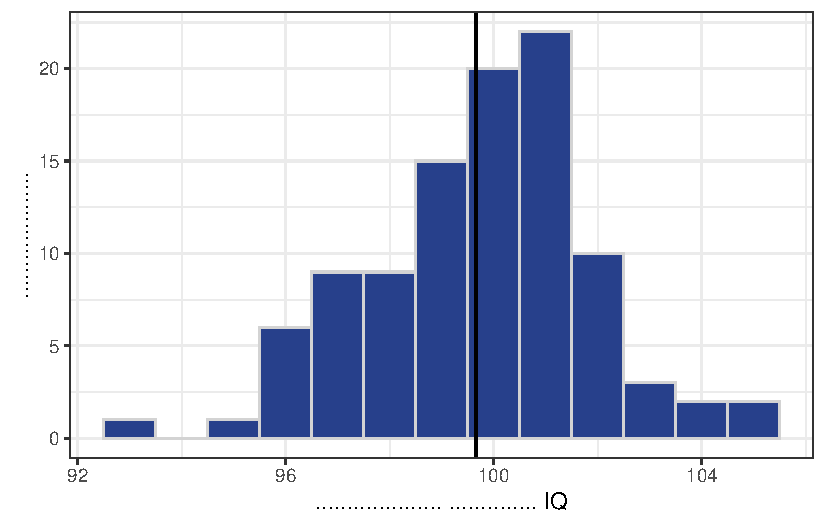
\includegraphics{stats-estim_files/figure-pdf/unnamed-chunk-5-1.pdf}

Наблюдаем, что иногда мы при подсчёте оценке параметра попадаем близко к
истинному его значению, иногда промахиваемся. Собственно, как раз об
этом \emph{неопределённость и вариация}.

\subsection{Метод
моментов}\label{ux43cux435ux442ux43eux434-ux43cux43eux43cux435ux43dux442ux43eux432}

Чтобы получить точечные оценки параметров, используются разные методы в
зависимости от конкретной модели анализа. Сейчас мы познакомимся с самым
простым --- \textbf{методом моментов}.

Само название метода отсылает нас к обсуждению
\hyperref[moments_distributions]{характеристик распределений случайных
величин}. Мы говорили о том, что распредления характеризуются их
\emph{моментами}. В методе моментов есть три этапа:

\begin{enumerate}
\def\labelenumi{\arabic{enumi})}
\tightlist
\item
  устанавливается связь между оцениваемым параметром и моментом
  распределения
\end{enumerate}

\[
\theta = \xi(\nu_k) \quad \text{или} \quad \theta = \xi(\mu_k)
\]

\begin{enumerate}
\def\labelenumi{\arabic{enumi})}
\setcounter{enumi}{1}
\tightlist
\item
  находятся выборочные моменты
\end{enumerate}

\[
\hat \theta = \xi(\nu_k^*) \quad \text{или} \quad \hat \theta = \xi(\mu_k^*)
\]

\begin{enumerate}
\def\labelenumi{\arabic{enumi})}
\setcounter{enumi}{2}
\tightlist
\item
  истинный момент заменяется на выборочный --- получается оценка.
\end{enumerate}

Для примера разберём всё тот же датасет с IQ. Мы знаем, что
распределение баллов IQ подчинается
\hyperref[normal_distribution]{нормальному закону}. Поэтому в качестве
параметра «среднее значение коэффициента интеллекта» генеральной
совокупности можно использовать математическое ожидание:

\[
\mu = \mathbb{E}X
\]

Выборочным аналогом математического ожидания является выборочное
среднее:

\[
\hat \mu = \frac{1}{n} \sum_{i=1}^n x_i
\]

И это, собственно, всё. Если вы хотя бы раз анализировали данные, вы
имплицитно пользовались этим знанием. Просто, скорее всего, не
задумывались, что это так работает. :)

\subsection{Метод максимального
правдоподобия}\label{ux43cux435ux442ux43eux434-ux43cux430ux43aux441ux438ux43cux430ux43bux44cux43dux43eux433ux43e-ux43fux440ux430ux432ux434ux43eux43fux43eux434ux43eux431ux438ux44f}

\subsection{Bootstrap}\label{bootstrap}

\subsection{Свойства точечных
оценок}\label{ux441ux432ux43eux439ux441ux442ux432ux430-ux442ux43eux447ux435ux447ux43dux44bux445-ux43eux446ux435ux43dux43eux43a}

Так как точечные оценки всё же оценки, мы можем и промахнуться мимо
истинного среднего --- это мы наблюдали на гистограмме. Поэтому нам надо
предъявить определённые требования к точечным оценкам. Их три:
\emph{несмещённость}, \emph{состоятельность} и \emph{эффективность}.

\subsubsection{Несмещенность}\label{ux43dux435ux441ux43cux435ux449ux435ux43dux43dux43eux441ux442ux44c}

\textbf{Несмещённость} выражает следующую идею: когда мы рассчитываем
выборочную оценку, мы должны как можно ближе попадать в истинное
значение параметра.

\[
\forall n \; \mathbb{E} \hat \theta = \theta, \quad (\mathbb{E}\hat \theta - \theta) \rightarrow 0,
\] где \(n\) --- объём выборки, \((\mathbb{E}\hat \theta - \theta)\) ---
смещение.

Слева представлено требование \emph{несмещённости при любом объёме
выборки}, а справа --- \emph{ассимптотической несмещённости}.

\paragraph{Проверка среднего как оценки математического ожидания на
несмещенность}\label{ux43fux440ux43eux432ux435ux440ux43aux430-ux441ux440ux435ux434ux43dux435ux433ux43e-ux43aux430ux43a-ux43eux446ux435ux43dux43aux438-ux43cux430ux442ux435ux43cux430ux442ux438ux447ux435ux441ux43aux43eux433ux43e-ux43eux436ux438ux434ux430ux43dux438ux44f-ux43dux430-ux43dux435ux441ux43cux435ux449ux435ux43dux43dux43eux441ux442ux44c}

\[ 
X_1, X_2, \dots , X_n \overset{\iid}{\thicksim} (\mu, \sigma^2)
\]

\[
\hat \mu = \frac{1}{m}\sum_{j=1}^m x_j = \bar X 
\]

\[
\expect (\hat \mu) = \expect (\bar X) \overset{?}{=} \mu
\]

\[
\expect (\bar X) = \expect \big (\frac{1}{n} \sum_{i=1}^n X_i \big ) = \frac{1}{n} \expect \Big( \sum_{i=1}^n X_i \Big) = \frac{1}{n} \sum_{i=1}^n \expect X_i \overset{X_i \overset{\iid}{\sim} (\mu, \sigma^2)}{=} \frac{1}{n} \cdot n \cdot \expect X = \frac{n}{n} \cdot \mu = \mu
\]

\paragraph{Проверка дисперсии генеральной совокупности как оценки
дисперсии на
несмещенность}\label{ux43fux440ux43eux432ux435ux440ux43aux430-ux434ux438ux441ux43fux435ux440ux441ux438ux438-ux433ux435ux43dux435ux440ux430ux43bux44cux43dux43eux439-ux441ux43eux432ux43eux43aux443ux43fux43dux43eux441ux442ux438-ux43aux430ux43a-ux43eux446ux435ux43dux43aux438-ux434ux438ux441ux43fux435ux440ux441ux438ux438-ux43dux430-ux43dux435ux441ux43cux435ux449ux435ux43dux43dux43eux441ux442ux44c}

\[ 
X_1, X_2, \dots , X_n \overset{\iid}{\thicksim} (\mu, \sigma^2)
\]

\[
\begin{split}
\disp X & = \sigma^2 = \expect(X - \expect X)^2 = \expect (X^2 - 2 X \expect X + \expect^2 X) = \\
& = \expect X^2 - 2\expect X \expect X + \expect^2 X = \expect X^2 - 2\expect^2 X + \expect^2 X = \\
& = \expect X^2 - \expect^2 X
\end{split}
\]

\[
\hat \sigma^2 = \frac{\sum_{i=1}^n (x_i - \bar X)^2}{n}
\]

\[
\expect (\hat \sigma^2) \overset{?}{=} \sigma^2
\]

\[
\begin{split}
\expect (\hat \sigma^2) & = \frac{\sum_{i=1}^n (x_i - \bar X)^2}{n} = \\
& = \frac{1}{n} \lp \sum_{i=1}^n x_i^2 - 2 \sum_{i=1}^n x_i \bar X  + \sum_{i=1}^n \bar X \rp \\ 
& = \frac{1}{n} \lp \sum_{i=1}^n x_i^2 - 2 \bar X \sum_{i=1}^n x_i + n \bar X \rp = \\
& = \frac{\sum_{i=1}^n x_i^2}{n} - 2 \bar X \frac{\sum_{i=1}^n x_i}{n} + \bar X^2 = \\
& = \overline{X^2} - 2 \bar X^2 + \bar X^2 = \overline{X^2} - \bar X^2
\end{split}
\]

\[
\expect (\hat \sigma^2) = \expect (\overline {X^2} - \bar X^2) = \underset{[1]}{\expect \overline{X^2}} - \underset{[2]}{\expect \bar X^2}
\]

\[
\begin{split}
[1] \, \expect \overline{X^2} : & \\
\expect \overline{X^2} & = \expect \lp \frac{\sum_{i=1}^n X_i^2}{n} \rp = \frac{1}{n} \expect \lp \sum_{i=1}^n X_i^2 \rp = \\
& = \frac{1}{n} \sum_{i=1}^n \expect X_i^2] \overset{X_i \overset{\iid}{\sim} (\mu, \sigma^2)}{=} \frac{1}{n} \cdot n \cdot \expect X^2 = \expect X^2
\end{split}
\]

\[
\begin{split}
[2] \, \expect \bar X^2 : & \\
\expect \bar X^2 & = 
\expect \lb 
    \lp \frac{\sum_{i=1}^n X_i}{n} \rp ^2 
  \rb = 
\frac{1}{n^2} 
\expect \lb 
    \lp \sum_{i=1}^n X_i^2 \rp 
  \rb = \\
& = \frac{1}{n^2} \expect \lb 
    \sum_{i=1}^n \expect X_i^2 + 
    2 \sum_{
      \substack{i=1, j=1 \\ i \neq j}
      }^n X_i X_j 
    \rb = \\
& = \frac{1}{n^2} \lb
      \sum_{i=1}^n \expect (X_i^2) + 
      2 \sum_{
        \substack{i=1, j=1 \\ i \neq j}
      }^n \expect (X_i X_j)
    \rb = \\
& \overset{X_i \overset{\iid}{\sim} (\mu, \sigma^2)}{=} \frac{1}{n^2} \lb 
    n \cdot \expect X^2 + 
    2 \sum_{
      \substack{i=1, j=1 \\ i \neq j}
    }^n \expect (X_i) \expect (X_j) \rb = \\
& = \frac{1}{n} \lb n \cdot \expect X2 + 2 \cdot \frac{n(n-1)}{2} \expect^2 X \rb  = \\
& = \frac{1}{n} \expect X^2 + \frac{n-1}{n} \expect^2 X
\end{split}
\]

\[
\begin{split}
\expect (\hat \sigma^2) 
& = \expect \overline{X^2} - \expect \bar X^2 = \\
& = \expect X^2 - \lp \frac{1}{n} \expect X^2 + \frac{n-1}{n} \expect^2 X \rp = \\
& = \frac{n}{n} \expect X^2 - \frac{1}{n} \expect X^2 - \frac{n-1}{n} \expect^2 X = \\
& = \frac{n-1}{n} \expect X^2 - \frac{n-1}{n} \expect^2 X = \frac{n-1}{n} \lp \expect X^2 - \expect ^2 X \rp \\ 
& = \frac{n-1}{n} \sigma^2
\end{split}
\]

\[
s^2 = \frac{n}{n-1} \sigma^2 = \frac{n}{n-1} \cdot \frac{1}{n} \cdot \sum_{i=1}^n (x_i - \bar X) = \frac{1}{n-1} \sum_{i=1}^n (x_i - \bar X)
\]

\subsubsection{Состоятельность}\label{ux441ux43eux441ux442ux43eux44fux442ux435ux43bux44cux43dux43eux441ux442ux44c}

Математически \textbf{состоятельность} определяется следующим образом:

\[
\lim_{n \rightarrow \infty} \prob (|\hat \theta - \theta| < \varepsilon) = 1, \, \varepsilon > 0
\]

Содержательно эта запись нам говорит следующее, что при неограниченном
росте мощности выборки наша оценка стремится к истинному значению
параметра. Может быть, такая формулировка не совсем точна математически,
но позволяет представить, что происходит.

\subsubsection{Эффективность}\label{ux44dux444ux444ux435ux43aux442ux438ux432ux43dux43eux441ux442ux44c}

Эффективность точечной оценки определяется достаточно просто. Так как
оценка параметра --- это случайная величина, но у неё есть
\emph{дисперсия}. Чтобы оценка была \textbf{эффективна}, её дисперсия
должна быть минимальной:

\[
\sigma^2_{\hat \theta} = \min
\]

Пример несмещённой, состоятельной и эффективной оценки --- это
выборочное среднее для оценки математического ожидания нормально
распределённой величины. Именно то, что мы и делали в примере применения
метода моментов.

\section{Интервальные
оценки}\label{ux438ux43dux442ux435ux440ux432ux430ux43bux44cux43dux44bux435-ux43eux446ux435ux43dux43aux438}

Кроме самого значения оценки, необходимо определить качество этой
оценки, иначе говоря --- её точность. Для этого используется такая
величина как \textbf{надёжность}:

\[
\gamma = \mathrm{P}(\theta_\min < \theta < \theta_\max)
\]

Такая форма оценки называется \textbf{интервальной оценкой параметра},
так как мы указываем \emph{интервал}, в котором находится истинное
значение с определённой вероятностью.

Такая форма оценки даёт исчерпывающую информацию о параметре: мы знаем
(1) интервал, в котором находится значение параметра генеральной
совокупности, а также (2) надёжность, с которой выбранный интервал
накрывает это значение.

Значение надежности \(\gamma\) может быть выбрано произвольно, но обычно
оно близко к единице. Однако необхожимо помнить, что чем выше
надёжность, тем шире границы интервальной оценки.

\subsection{Стандартная
ошибка}\label{ux441ux442ux430ux43dux434ux430ux440ux442ux43dux430ux44f-ux43eux448ux438ux431ux43aux430}

\subsubsection{\texorpdfstring{Почему
\(\se(X) = \frac{\sd(X)}{\sqrt{n}}\)}{Почему \textbackslash se(X) = \textbackslash frac\{\textbackslash sd(X)\}\{\textbackslash sqrt\{n\}\}}}\label{ux43fux43eux447ux435ux43cux443-sex-fracsdxsqrtn}

\[
\var (X + Y) = \var (X) + \var(Y) + 2 \cov (X, Y)
\]

\[
\var (aX) = a^2 \var (X)
\]

Так как наблюдения извлекаются из независимых одинаково распределенных
величин (independent identically distributed, iid), то

\[
\cov (X_i, X_j) = 0, \sigma_{X_i} = \sigma_{X_j} = \sigma
\]

\[
\var \Big( \frac{1}{n} \sum X_i \Big) = \frac{1}{n^2} \sum \var(X_i) = \frac{1}{n^2} \sum \sigma^2 = \frac{n}{n^2} \sigma^2 = \frac{\sigma^2}{n}
\]

\[
\se_X = \sqrt{ \var \Big( \frac{1}{n} \sum X_i \Big)} = \sqrt{\frac{\sigma^2}{n}} = \frac{\sigma}{\sqrt{n}}
\]

\subsection{Доверительный
интервал}\label{ux434ux43eux432ux435ux440ux438ux442ux435ux43bux44cux43dux44bux439-ux438ux43dux442ux435ux440ux432ux430ux43b}

Вариантом интервальной оценки является \textbf{доверительный интервал
(confidence interval)}. Итак, ещё раз:

\[
\mathrm{P}(\theta_\min < \theta < \theta_\max) = \gamma, \; \gamma \rightarrow 1
\]

\(theta_\min\) и \(\theta_\max\) --- границы доверительного интервала,
\(\gamma\) --- доверительная вероятность. На практике её значение чаще
всего принимается равным \(0.95\).

\textbf{Алгоритм определения интервальной оценки} следующий:

\begin{enumerate}
\def\labelenumi{\arabic{enumi})}
\tightlist
\item
  Найсти статистику \(\zeta(\theta)\), связанную с оцениваниемым
  параметром, закон распределения которой известен \(f(\zeta)\).
\item
  Определить значения \(\zeta_\min\) и \(\zeta_\max\), в пределах
  которых статистика находится с вероятностью \(\gamma\).
\item
  Зная связь \(\zeta(\theta)\) перейти к границам \(\theta_\min\) и
  \(\theta_\max\).
\end{enumerate}

Разберемся с этим на примере построения доверительного интервала для
генерального среднего.

Первая задача --- найти статистику. Мы воспользуемся тем, что за нас
поработали учёные-статистики и сказали, что вот такая вполне подойдёт:

\[
t = \frac{\bar x - \mu}{s}\sqrt{n-1},
\]

где \(t\) --- значение статистики, \(\bar x\) --- выборочное среднее,
\(\mu\) --- генеральное среднее, \(s\) --- выборочное стандартное
отклонение, \(n\) --- объём выборки.

Известен ли закон её распредления? Да. Эта статистика подчинается
\(t\)-распределению (распределению Стьюдента). Оно похоже на нормальное,
но хвосты у него повыше:

Теперь надо сформулировать вид интервальной оценки для генерального
среднего. Путем арифметических преобразований формулы выше мы имеет
следующее:

\[
\mu = \bar x - t \frac{s}{\sqrt{n-1}}
\]

Значит вид интервальной оценки будет таков:

\[
\mathrm{P}\Big( \bar x - t_\alpha \frac{s}{\sqrt{n-1}} < \mu < 
\bar x + t_\alpha \frac{s}{\sqrt{n-1}}\Big) = 1 - \alpha = \gamma
\]

Посмотрим на картинку:

Видим на ней наш доверительный интвервал и значения \(t_\alpha\) и
\(-t_\alpha\). Сама \(\alpha\) обозначает вероятность выхода за границы
доверительного интервала. Осталось всё это высчитать в числах, и
получить границы доверительного интервала.

Хорошо, что весь этот ужас в R скрыт под капотом:

\begin{Shaded}
\begin{Highlighting}[]
\FunctionTok{mean\_cl\_normal}\NormalTok{(iq}\SpecialCharTok{$}\NormalTok{IQ)}
\end{Highlighting}
\end{Shaded}

\begin{verbatim}
         y     ymin     ymax
1 100.0063 99.71275 100.2999
\end{verbatim}

\begin{Shaded}
\begin{Highlighting}[]
\FunctionTok{mean\_cl\_boot}\NormalTok{(iq}\SpecialCharTok{$}\NormalTok{IQ)}
\end{Highlighting}
\end{Shaded}

\begin{verbatim}
         y     ymin     ymax
1 100.0063 99.72359 100.3098
\end{verbatim}

\bookmarksetup{startatroot}

\chapter{Тестирование статистических гипотез}\label{stats-testing}

В ходе статистического анализа мы, главным образом, заняты тем, что
тестируем статистические гипотезы. Ведь на какого рода вопросы мы
отвечаем с помощью анализа?

\begin{itemize}
\tightlist
\item
  Различаются ли группы между собой?
\item
  Значимо ли влияние какого-либо фактора? → Различаются ли группы между
  собой?
\item
  Хороша ли та модель, которую мы построили? → Отличается ли она от
  нулевой модели?
\end{itemize}

И так далее. Так или иначе, всё сводится в тому, что мы ищем какие-то
различия. Но силу того, что у нас неопределённость и вариация в данных,
мы просто так «в лоб» сказать о различиях по оценкам параметров не
можем. Приходится тестировать статистические гипотезы.

\section{Нулевая и альтернативная
гипотезы}\label{stats-testing-hyotheses}

Еще раз тезисно \hyperref[stats-hypotheses]{вспомним о гипотезах} в
целом:

\begin{itemize}
\tightlist
\item
  \textbf{Гипотеза} (\(H\)) --- это предположение, которое подлежит
  проверке на основе результатов наблюдений.
\item
  Гипотезы бывают:

  \begin{itemize}
  \tightlist
  \item
    \textbf{теоретические} --- про конструкты
  \item
    \textbf{эмпирические} --- про переменные
  \item
    \textbf{статистические} --- про параметры {[}генеральной
    совокупности{]} и данные
  \end{itemize}
\end{itemize}

Статистические гипотезы бывают простыми и сложными:

\begin{itemize}
\tightlist
\item
  \textbf{Простая гипотеза} --- это такое предположение, которое
  включает в себя какое-либо однозначно определеяемое утверждение.
  Например, истинная величина параметра соответствует некоторому строго
  заданному значению: \(H : \theta = \theta_0\). Другой вариант --- две
  генеральные совокупности имеют одно и то же значение одной и той же
  характеристики: \(H : \theta_1 = \theta_2\).
\item
  \textbf{Сложная гипотеза} предполагает множественность вариантов для
  параметра, которые укладываются в рамки проверяемого предположения.
  Например, \(H : \theta > \theta_0\) или
  \(H : \theta_1 \neq \theta_2\).
\end{itemize}

В рамках самого хода тестирования гипотез существует \textbf{проверяемая
(нулевая) гипотеза} (\(H_0\)). Её обычно стараются предельно упростить,
поэтому она формулируется как простая гипотеза. В противовес ей
выдвигается \textbf{альтернативная гипотеза} (\(H_1\)), которая будет
иметь вид сложной гипотезы.

Для проверки гипотезы необходимы две вещи:

\begin{itemize}
\tightlist
\item
  результаты наблюдений и
\item
  критерий.
\end{itemize}

Результаты наблюдений, полученные на выборке, сами по себе, как правило,
не используются. Однако на их основе рассчитываются выборочные
статистики (показатели), которые непосредственно участвуют в проверке
гипотезы.

\section{Подходы к тестированию статистических
гипотез}\label{stats-testing-approaches}

\subsection{Фреквентистский подход}\label{stats-testing-nhst}

\subsection{Байесовский подход}\label{stats-testing-bayes}

\section{Возможные результаты проверки
гипотез}\label{stats-testing-results}

В результате проверки статистических гипотез могут возникнуть четыре
ситуации.

Мы изучаем в исследовании какую-либо закономерность, которая в реальном
мире может существовать, а может и не существовать. В силу
неопределённости и вариативности наших данных мы может либо обнаружить
интересующую нас закономерность, либо не обнаружить.

В качестве нулевой гипотезы мы выдвигаем предположение о том, что
закономерность отсутствует --- так мы упрощаем нашу нулевую гипотезу.
Пусть \(H_0\) обозначает, что предположение, которое мы проверяем
справедливо, а \(H_1\) --- не справедливо. На основании данных мы можем
либо не отклонить наше предположение (\(\hat H_0\)), либо отклонить
(\(\hat H_1\)).

Тогда имеем следующую ситуацию:

\begin{longtable}[]{@{}ccc@{}}
\toprule\noalign{}
& \(H_0\) & \(H_1\) \\
\midrule\noalign{}
\endhead
\bottomrule\noalign{}
\endlastfoot
\(\hat H_0\) & ✓ & Ошибка II рода \\
\(\hat H_1\) & Ошибка I рода & ✓ \\
\end{longtable}

\begin{itemize}
\tightlist
\item
  \textbf{Ошибка I рода} возникает, когда в генеральной совокупности
  \emph{искомой закономерности нет}, но мы в силу случайных флуктуаций в
  данных \emph{её нашли}.
\item
  \textbf{Ошибка II рода} возникает, когда в генеральной совокупности
  \emph{искомая закономерность есть}, но мы в силу каких-либо причин её
  \emph{не нашли}.
\end{itemize}

Ошибки --- это нехорошо, они нас не устраивают. Надо каким-то образом их
контролировать.

\begin{itemize}
\tightlist
\item
  \textbf{Ошибка I рода} контролируется достаточно просто. Так как мы
  \emph{нашли} закономерность, которую искали, мы можем посчитать
  вероятность, с которой потенциально ошиблись. А собственно
  контролировать ошибку мы будем с помощью \textbf{уровня значимости}
  \(\alpha\), который \emph{выбирается до начала процедуры тестирования
  гипотезы}. Он и задает вероятность, с который мы позволяем себе
  ошибиться --- отклонить нулевую гипотезу, при условии, что она верна.
\item
  \textbf{Ошибку II рода} контролировать сложнее, так как мы \emph{не
  нашли} закономерность, которую искали. Нам нужна какая-то метрика,
  которая позволит сказать, что мы сделали всё возможное для того, чтобы
  обнаружить искомую закономерность. Вероятность ошибки II рода
  обозначается \(\beta\) --- тогда вероятность того, что мы не совершили
  ошибку II рода будет \(1 - \beta\). Эта величина называется
  \hyperref[stats-testing-effect-size]{\textbf{статистической
  мощностью}}, и она связана с
  \hyperref[stats-testing-effect-size]{\emph{размером эффекта}} и
  \emph{объемом выборки}. Статистическую мощность можно рассчитать как
  до проведения статистического анализа для расчета требуемого объема
  выборки --- так и после --- для определения достигнутой статистической
  мощности.
\end{itemize}

Соберем все обозначения в единую табличку\footnote{Здесь использовано
  обозначение условной вероятности \(\mathrm P(A|B)\), то есть это
  вероятность того, что случилось событие \(A\) при условии, что
  случилось событие \(B\).}:

\begin{longtable}[]{@{}
  >{\centering\arraybackslash}p{(\columnwidth - 4\tabcolsep) * \real{0.1714}}
  >{\centering\arraybackslash}p{(\columnwidth - 4\tabcolsep) * \real{0.4286}}
  >{\centering\arraybackslash}p{(\columnwidth - 4\tabcolsep) * \real{0.4000}}@{}}
\toprule\noalign{}
\begin{minipage}[b]{\linewidth}\centering
\end{minipage} & \begin{minipage}[b]{\linewidth}\centering
\(H_0\)
\end{minipage} & \begin{minipage}[b]{\linewidth}\centering
\(H_1\)
\end{minipage} \\
\midrule\noalign{}
\endhead
\bottomrule\noalign{}
\endlastfoot
\(\hat H_0\) & \(\mathrm P (\hat H_0 | H_0)\) &
\(\mathrm P (\hat H_0 | H_1) = \beta\) \\
\(\hat H_1\) & \(\mathrm P (\hat H_1 | H_0) = \alpha\) &
\(\mathrm P (\hat H_1 | H_1) = 1 - \beta\) \\
\end{longtable}

Уровень значимости \(\alpha\) \textbf{выбирается близким к нулю} ---
всем знакомо конвенциональное значение \(0.05\). Вообще \(\alpha\) можно
выбрать сколь угодно малым, однако при выборе уровня значимости
руководствуются принципом разумной достаточности, так как если устремить
\(\alpha\) к нулю, то устремиться к нулю и вероятность отклонения
нулевой гипотезы.

\emph{Математические руны}

\[
\mathrm P (\hat H_1) = \mathrm P (\hat H_1 | H_0) \cdot \mathrm P (H_0) = \alpha \cdot \mathrm P(H_0)
\]

Достаточной статистической мощностью считается \(0.8\). Аналогично,
устремляя мощность к единице
(\((1 - \beta) \rightarrow 1 \Rightarrow \beta \rightarrow 0\)), мы
устремляем вероятность не отклонения нулевой гипотезы к нулю:

\emph{Ещё математические руны}

\[
\mathrm P (\hat H_0) = \mathrm P (\hat H_0 | H_1) \cdot \mathrm P (H_1) = \beta \cdot \mathrm P (H_1)
\]

Необходимо также помнить, что ошибки первого и второго рода связаны
между собой так, что

\[
\alpha \rightarrow 0 \Rightarrow \beta \rightarrow 1
\]

\emph{Опять математические руны}

\[
\beta \cdot \mathrm P (H_1) = \mathrm P (\hat H_0) = \mathrm P (\hat H_0 | H_0) \cdot \mathrm P (H_0) \Rightarrow \beta = \frac{1}{\mathrm P (H_1)} \cdot \mathrm P (H_0) \cdot \mathrm P(\hat H_0 | H_0) \\
\beta = \frac{1}{\mathrm P (H_1)} \cdot \big (1 - \mathrm P (H_1 | H_0)\big) = \frac{1}{\mathrm P (H_1)} \cdot \mathrm P (H_0) \cdot (1 - \alpha)
\]

\subsection{Асимметрия статистического
вывода}\label{stats-testing-asymmetry}

Выше мы сказали, что для проверки гипотезы нужны две вещи:

\begin{itemize}
\tightlist
\item
  результаты наблюдений и
\item
  критерий.
\end{itemize}

С результатами наблюдений более-менее очевидно.

\textbf{Критерий} --- это правило, согласно которому гипотезу либо
принимают, либо отклоняют. Однако перед тем как проверять гипотезу, её
так-то нужно сформулировать, и сделать это правильно, поскольку от
формулировки гипотезы зависит интерпретация результатов проверки и
дальнейшее использование полученной информации.

Используемая статистика сама по себе является {[}непрерывной{]}
случайной величиной, а значит может быть построено её распределение.
Критерий будет разделять это распределение на непересекающиеся области.
В результате чего возникает \textbf{критическая область} --- область
отклонения гипотезы. Дополнением к ней является область неотклонения
гипотезы.

Критическая область может быть односторонней (при
\(H_1:\theta > \theta_0\) или \(H_1: \theta < \theta_0\)) и двусторонней
(при \(H_1:\theta \neq \theta_0\)). «Размер» критической области
определяется \textbf{уровнем значимости}.

Статистический вывод --- заключение о том, получили ли мы подтверждение
альтернативной гипотезы --- по структуре представляет собой
\emph{импликацию}. Если вам не знаком этот термин из логики, то вот:

\begin{itemize}
\tightlist
\item
  Если значение нашей статистики, которое мы рассчитали на выборке,
  \emph{попало в критическую область}, то мы говорим о том, что
  \emph{нулевая гипотеза отклоняется}.
\item
  Если значение нашей статистики, которое мы рассчитали на выборке,
  \emph{не попало в критическую область}, то мы \emph{не получаем
  оснований для того, чтобы отклонить нулевую гипотезу}. Однако \emph{мы
  также не получаем оснований, чтобы её «принять»}. Мы остаёмся в
  некотором неведении: мы не нашли различий, а есть они там или нет ---
  хто ж их знает\ldots{} Итого, мы не можем сделать никакого вывода.
\end{itemize}

В этом и заключается асимметрия статистического вывода. Как раз для
того, чтобы с ней как-то жить, мы работаем со статистической мощностью.

\begin{center}\rule{0.5\linewidth}{0.5pt}\end{center}

Посмотреть, как все эти штуки друг с другом соотносятся можно
\href{https://rpsychologist.com/d3/nhst/}{тут}.

\begin{center}\rule{0.5\linewidth}{0.5pt}\end{center}

\subsection{Связь ошибки первого и второга
рода}\label{stats-testing-errors-connection}

\section{Агоритм тестирования статистических
гипотез}\label{stats-testing-algorithm}

Для тестирования гипотез есть два сценария: \emph{первый} и \emph{тот,
которым мы будем пользоваться}. Первый вариант чуть более классический,
второй --- более гибкий.

\textbf{Сценарий номер раз}

\begin{enumerate}
\def\labelenumi{\arabic{enumi}.}
\tightlist
\item
  Формулировка гипотезы
\item
  Выбор статистического критерия
\item
  Выбор уровня значимости \(\alpha\)
\item
  Построение закона распредления статистики критерия при условии, что
  нулевая гипотеза верна
\item
  Определение границ критической области
\item
  Расчёт выборочной статистики
\item
  Определение, попадает ли наблюдемое значение статистики в критическую
  область и вынесение решения
\end{enumerate}

\textbf{Сценарий номер два}

\begin{enumerate}
\def\labelenumi{\arabic{enumi}.}
\tightlist
\item
  Формулировка гипотезы
\item
  Выбор статистического критерия
\item
  Выбор уровня значимости \(\alpha\)
\item
  Построение закона распредлеения статистики критерия при условии, что
  нулевая гипотеза верна
\item
  Расчёт выборочной статистики
\item
  Расчёт достигнутого уровня значимости \emph{p-value}
\item
  Сопоставление \(\alpha\) и \emph{p-value} и вынесение решения
\end{enumerate}

Почему второй вариант более гибкий? Представим, что мы захотели понизить
уровень значимости с \(0.05\) до \(0.01\) --- такие уровни значимости
всречаются, например, в медицине. Если мы идем по первому сценарию, то
нам надо заново пересчитать критические значения и вновь
проанализировать, попадает ли наблюдаемое значение в критическую
область. Если мы адепты второго сценария, то нам надо только выполнить
одно новое сравнение нашего \emph{p-value} с новым уровнем значимости.

\section{Размер эффекта}\label{stats-testing-effect-size}

\section{Статистическая мощность}\label{stats-testing-power}

\begin{tcolorbox}[enhanced jigsaw, colback=white, bottomrule=.15mm, opacityback=0, opacitybacktitle=0.6, breakable, coltitle=black, colframe=quarto-callout-note-color-frame, titlerule=0mm, rightrule=.15mm, bottomtitle=1mm, leftrule=.75mm, toptitle=1mm, left=2mm, arc=.35mm, title=\textcolor{quarto-callout-note-color}{\faInfo}\hspace{0.5em}{Статистическая мощность Post hoc}, colbacktitle=quarto-callout-note-color!10!white, toprule=.15mm]

НАПИСАТЬ

есть ли смысл рассчитывать статистическую мощность пост хок?

кажется, нет, так как эффект уже нашли

\end{tcolorbox}

\section{Ложноположительный вывод}\label{stats-testing-false-positive}

\subsection{Проблема множественных
сравнений}\label{stats-testing-multiple-comparisons}

Итак, мы сравниваем попарно все группы наблюдений между собой. В каждом
сравнении мы фиксируем вероятность ошибки первого рода с помощью уровня
значимости на уровне \(0.05\). А какова будет вероятность ошибки, если
мы проводим несколько сравнений?

Считаем, что наши сравнения независимы, поэтому вероятности будут
перемножаться1. Если верояность ошибиться в одном сравнении равна
\(\alpha\), то вероятность сделать правильный вывод --- \(1 - \alpha\).
Тогда вероятность сделать правильный вывод в \(m\) сравнениях ---
\((1 - \alpha)^m\). Отсюда мы можем вывести вероятность ошибиться хотя
бы в одном сравнении:

\[
\prob^′ = 1 - (1 - \alpha)^m
\]

Пусть у нас есть три группы, которые нам надо сравнить друг с другом ---
получается необходимо провести три сравнения. Итого вероятность
ошибиться получается:

\[
\prob^′ = 1 - (1 - 0.05)^3 \approx 0.143
\]

Значительно больше, чем \(0.05\), что нехорошо. И дальше только хуже.
Поэтому нам надо либо корректировать уровень значимости, либо
использовать мощные методы типа дисперсионного анализа.

\begin{figure}[H]

{\centering 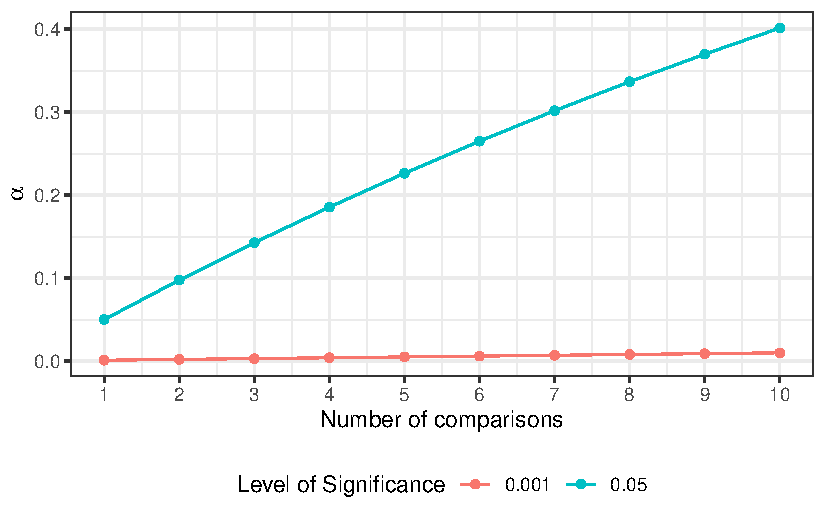
\includegraphics{stats-testing_files/figure-pdf/alpha-raise-1.pdf}

}

\caption{Рост вероятности ошибки первого рода при увеличении числа
попарных сравнений}

\end{figure}%

\subsubsection{Корректировка уровня
значимости}\label{stats-testing-correction}

Корректировать уровень значимости можно по-разному. Например, можно
разделить \(\alpha\) на количество попарных сравнений --- такой способ
называется поправкой Бонферрони (Bonferroni):

\[
\alpha’ = \frac{\alpha}{n},
\]

где \(n\) --- число попарных сравнений.

Поправка Бонферрони считается самой консервативной поправкой --- она
достаточно сильно уменьшает уровень значимости, и мы можем не поймать
искомую закономерность, то есть совершить ошибку второго рода2. Поэтому
придумали более либеральные поправки, например, поправку Холма
(Холма--Бонферрони, Holm) или поправку Тьюки (Tukey's HSD test). Можно
посмотреть на их формулы, но в целом, не обяз, потому что их все равно
никто не знает, а в статистических пакетах мы либо допишем аргумент в
функцию, либо нужную галку поставим.

На практике в силу того, что в статистических пакетах мы работаем с
p-value, корректируется именно его значение.

По достаточно незамысловатой логике Здесь: вариант для поправки
Бонферрони.

\[
p < \frac{\alpha}{n} \Rightarrow np < \alpha
\]

Таким образом, мы просто сравниваем уже скорретированное p-value,
которое нам считает программа, с тем же самым \(\alpha = 0.05\). Жизнь
становится значительно проще и приятнее.

\subsection{Проблема количества статистических
тестов}\label{stats-testing-multiple-testing}

\part{Методы анализа данных}

\bookmarksetup{startatroot}

\chapter{Описательные статистики}\label{andan-descriptives}

\section{Виды статистики}\label{andan-descriptives-kinds-of-stats}

Напомним себе, что статистика {[}как набор методов и инструментов{]}
делится на два вида --- описательная статистика и статистика вывода.

\begin{itemize}
\tightlist
\item
  \textbf{Описательная статистика (descriptive statistics\footnote{Mass
    (uncountable) noun})} занимается обработкой статистических данных,
  их наглядным представлением, и собственно описанием через некоторые
  характеристики.

  \begin{itemize}
  \tightlist
  \item
    Эти характеристики, количественно описывающие особенности имеющихся
    данных, называются \textbf{описательными статистиками (descriptive
    statistics\footnote{Countable noun, plural in this case})}.
  \item
    \emph{Задача описательной статистики} --- ёмко описать имеющиеся
    данные и составить на основе этих описаний общее представление о
    них, а также обнаружить особенности, которые могут повлиять на
    дальнейший анализ.
  \end{itemize}
\item
  \textbf{Статистика вывода (inferential statistics)} занимается поиском
  ответов на содержательные вопросы, которые мы задаем данным в ходе их
  анализа в рамках научных и практических исследований.

  \begin{itemize}
  \tightlist
  \item
    Состоит из двух компонентов --- \emph{тестирования статистических
    гипотез} и \emph{статистических методов}.
  \end{itemize}
\end{itemize}

\begin{tcolorbox}[enhanced jigsaw, colback=white, bottomrule=.15mm, opacityback=0, opacitybacktitle=0.6, breakable, coltitle=black, colframe=quarto-callout-note-color-frame, titlerule=0mm, rightrule=.15mm, bottomtitle=1mm, leftrule=.75mm, toptitle=1mm, left=2mm, arc=.35mm, title=\textcolor{quarto-callout-note-color}{\faInfo}\hspace{0.5em}{Замечание о машинном обучении}, colbacktitle=quarto-callout-note-color!10!white, toprule=.15mm]

В названии книги упомянуто «машинное обучение». Иногда его причисляют к
статистике, иногда рассматривают отдельно. На самом же деле,
статистические методы лежат где-то между статистикой вывода и машинным
обучением.

Почему?

Дело в том, что на статистические методы можно смотреть по-разному.

\begin{itemize}
\tightlist
\item
  Если нашей задачей является поиск ответов на
  \textbf{исследовательские} вопросы о закономерностях, о связи
  каких-либо факторов или влиянии переменных друг на друга, то мы будем
  смотреть на статистические модели с точки зрения статистики вывода.
  Это позволит нам находить ответы на интересующие нас вопросы ---
  причем не важно, говорим мы о научных исследованиях или об
  исследованиях в индустрии.
\item
  Если перед нами стоит задача хорошо \textbf{предсказывать} одни
  переменные на основании значений других --- например, выдавать
  рекомендации на Яндекс.Музыке или в Яндекс.Лавке~--- то мы будем
  смотреть на те же статистические модели с точки зрения машинного
  обучения.
\end{itemize}

То есть, модели в анализе данных и машинном обучении одни и те же, но
то, какую модель мы назовем хорошей и как мы эту «хорошесть» определим,
будет отличаться в зависимости от задачи~--- \emph{исследовательская}
или \emph{предиктивная}~--- которая перед нами стоит.

\end{tcolorbox}

\section{Меры центральной
тенденции}\label{andan-descriptives-central-tendency}

Итак, мы хотим описать наши данные. Точнее, распределения переменных,
которые у нас в данных есть. Хотим сделать это просто и ёмко. Насколько
просто и ёмко? Ну, допустим максимально --- одним числом. Для этого
неплохо подойдет значение переменной, которое лежит \emph{в центре}
распределения.

Как мы будем искать, что там в центре распределения? Зависит от
\href{}{шкалы} \autocite{stevens46}, в которой измерена конкретная
переменная (Таблица~\ref{tbl-scales-cental-tendencies}).

\begin{longtable}[]{@{}
  >{\raggedright\arraybackslash}p{(\columnwidth - 2\tabcolsep) * \real{0.2500}}
  >{\raggedright\arraybackslash}p{(\columnwidth - 2\tabcolsep) * \real{0.7500}}@{}}
\caption{Шкалы и меры центральной
тенденции}\label{tbl-scales-cental-tendencies}\tabularnewline
\toprule\noalign{}
\begin{minipage}[b]{\linewidth}\raggedright
\textbf{Шкала}
\end{minipage} & \begin{minipage}[b]{\linewidth}\raggedright
\textbf{Мера центральной тенденции}
\end{minipage} \\
\midrule\noalign{}
\endfirsthead
\toprule\noalign{}
\begin{minipage}[b]{\linewidth}\raggedright
\textbf{Шкала}
\end{minipage} & \begin{minipage}[b]{\linewidth}\raggedright
\textbf{Мера центральной тенденции}
\end{minipage} \\
\midrule\noalign{}
\endhead
\bottomrule\noalign{}
\endlastfoot
\emph{Номинальная} & Мода \\
\emph{Порядковая} & Медиана \\
\emph{Интервальная} & Среднее арифметическое \\
\emph{Абсолютная} & Среднее арифметическое, геометрическое и др. \\
\end{longtable}

Однако есть некоторые нюансы.

\subsection{Мода}\label{andan-descriptives-mode}

Самый простой вариант найти центральную тенденцию --- это определить
наиболее часто встречающееся значение переменной. Это значение
называется \emph{модой (mode)}.

\begin{definition}[]\protect\hypertarget{def-mode-discrete}{}\label{def-mode-discrete}

\textbf{Мода} {[}дискретной переменной{]} --- наиболее часто
встречающееся значение данной переменной.

\end{definition}

Например, у нас есть следующий ряд наблюдений по какой-то переменной:

\[
\begin{bmatrix}
1 & 3 & 4 & 6 & 3 & 2 & 3 & 3 & 2 & 4 & 1
\end{bmatrix}
\]

Если мы посчитаем, сколько раз встретилась каждое значение переменной и
составим таблицу частот, то получим следующее:

\[
\begin{matrix}
\text{Значение} & 1 & 2 & 3 & 4 & 6 \\
\text{Частота}  & 2 & 2 & 4 & 2 & 1
\end{matrix}
\]

Очевидно, что \(3\) встречается чаще других значений --- это и есть
мода.

Понятно, что если на нашей шкале нет чисел, а есть текстовые лейблы, это
ничего не меняет. Пусть у нас есть переменная с кодами аэропортов:

\[
\begin{bmatrix}
\text{DME} & \text{LED} & \text{IST} & \text{AER} & \text{IST} &\text{SVO} & \text{LED} & \text{VKO} & \text{LED} & \text{IST} & \text{IST} & \text{VKO} & \text{AER} & \text{DME}
\end{bmatrix}
\]

\[
\begin{matrix}
\text{Значение} & \text{DME} & \text{LED} & \text{IST} & \text{AER} & \text{SVO} & \text{VKO}\\
\text{Частота}  & 2 & 3 & 4 & 2 & 1 & 2
\end{matrix}
\]

Мода --- \(\text{IST}\) (Международный аэропорт Стамбула, İstanbul
Havalimanı).

Так мы действуем в случае с эмпирическим распределением. Если нам
известна \href{}{функция вероятности переменной (probability mass
function, PMF)}, то мы можем определить моду, основываясь на ней:

\begin{definition}[]\protect\hypertarget{def-mode-discrete-pmf}{}\label{def-mode-discrete-pmf}

\textbf{Мода} {[}дискретной переменной{]} --- это значение переменной,
при котором её функция вероятности принимает своё максимальное значение.

\end{definition}

\begin{equation}\phantomsection\label{eq-mode-pmf}{
\text{mode}(X) = \arg \max(\text{PMF}(X)) = \arg \max_{x_i}(\prob (X = x_i)),
}\end{equation}

где \(X\) --- дискретная случайная величина, \(x_i\) --- значение этой
случайной величины.

\begin{verbatim}
Warning in grid.Call.graphics(C_text, as.graphicsAnnot(x$label), x$x, x$y, :
conversion failure on 'это максимум функции' in 'mbcsToSbcs': dot substituted
for <d1>
\end{verbatim}

\begin{verbatim}
Warning in grid.Call.graphics(C_text, as.graphicsAnnot(x$label), x$x, x$y, :
conversion failure on 'это максимум функции' in 'mbcsToSbcs': dot substituted
for <8d>
\end{verbatim}

\begin{verbatim}
Warning in grid.Call.graphics(C_text, as.graphicsAnnot(x$label), x$x, x$y, :
conversion failure on 'это максимум функции' in 'mbcsToSbcs': dot substituted
for <d1>
\end{verbatim}

\begin{verbatim}
Warning in grid.Call.graphics(C_text, as.graphicsAnnot(x$label), x$x, x$y, :
conversion failure on 'это максимум функции' in 'mbcsToSbcs': dot substituted
for <82>
\end{verbatim}

\begin{verbatim}
Warning in grid.Call.graphics(C_text, as.graphicsAnnot(x$label), x$x, x$y, :
conversion failure on 'это максимум функции' in 'mbcsToSbcs': dot substituted
for <d0>
\end{verbatim}

\begin{verbatim}
Warning in grid.Call.graphics(C_text, as.graphicsAnnot(x$label), x$x, x$y, :
conversion failure on 'это максимум функции' in 'mbcsToSbcs': dot substituted
for <be>
\end{verbatim}

\begin{verbatim}
Warning in grid.Call.graphics(C_text, as.graphicsAnnot(x$label), x$x, x$y, :
conversion failure on 'это максимум функции' in 'mbcsToSbcs': dot substituted
for <d0>
\end{verbatim}

\begin{verbatim}
Warning in grid.Call.graphics(C_text, as.graphicsAnnot(x$label), x$x, x$y, :
conversion failure on 'это максимум функции' in 'mbcsToSbcs': dot substituted
for <bc>
\end{verbatim}

\begin{verbatim}
Warning in grid.Call.graphics(C_text, as.graphicsAnnot(x$label), x$x, x$y, :
conversion failure on 'это максимум функции' in 'mbcsToSbcs': dot substituted
for <d0>
\end{verbatim}

\begin{verbatim}
Warning in grid.Call.graphics(C_text, as.graphicsAnnot(x$label), x$x, x$y, :
conversion failure on 'это максимум функции' in 'mbcsToSbcs': dot substituted
for <b0>
\end{verbatim}

\begin{verbatim}
Warning in grid.Call.graphics(C_text, as.graphicsAnnot(x$label), x$x, x$y, :
conversion failure on 'это максимум функции' in 'mbcsToSbcs': dot substituted
for <d0>
\end{verbatim}

\begin{verbatim}
Warning in grid.Call.graphics(C_text, as.graphicsAnnot(x$label), x$x, x$y, :
conversion failure on 'это максимум функции' in 'mbcsToSbcs': dot substituted
for <ba>
\end{verbatim}

\begin{verbatim}
Warning in grid.Call.graphics(C_text, as.graphicsAnnot(x$label), x$x, x$y, :
conversion failure on 'это максимум функции' in 'mbcsToSbcs': dot substituted
for <d1>
\end{verbatim}

\begin{verbatim}
Warning in grid.Call.graphics(C_text, as.graphicsAnnot(x$label), x$x, x$y, :
conversion failure on 'это максимум функции' in 'mbcsToSbcs': dot substituted
for <81>
\end{verbatim}

\begin{verbatim}
Warning in grid.Call.graphics(C_text, as.graphicsAnnot(x$label), x$x, x$y, :
conversion failure on 'это максимум функции' in 'mbcsToSbcs': dot substituted
for <d0>
\end{verbatim}

\begin{verbatim}
Warning in grid.Call.graphics(C_text, as.graphicsAnnot(x$label), x$x, x$y, :
conversion failure on 'это максимум функции' in 'mbcsToSbcs': dot substituted
for <b8>
\end{verbatim}

\begin{verbatim}
Warning in grid.Call.graphics(C_text, as.graphicsAnnot(x$label), x$x, x$y, :
conversion failure on 'это максимум функции' in 'mbcsToSbcs': dot substituted
for <d0>
\end{verbatim}

\begin{verbatim}
Warning in grid.Call.graphics(C_text, as.graphicsAnnot(x$label), x$x, x$y, :
conversion failure on 'это максимум функции' in 'mbcsToSbcs': dot substituted
for <bc>
\end{verbatim}

\begin{verbatim}
Warning in grid.Call.graphics(C_text, as.graphicsAnnot(x$label), x$x, x$y, :
conversion failure on 'это максимум функции' in 'mbcsToSbcs': dot substituted
for <d1>
\end{verbatim}

\begin{verbatim}
Warning in grid.Call.graphics(C_text, as.graphicsAnnot(x$label), x$x, x$y, :
conversion failure on 'это максимум функции' in 'mbcsToSbcs': dot substituted
for <83>
\end{verbatim}

\begin{verbatim}
Warning in grid.Call.graphics(C_text, as.graphicsAnnot(x$label), x$x, x$y, :
conversion failure on 'это максимум функции' in 'mbcsToSbcs': dot substituted
for <d0>
\end{verbatim}

\begin{verbatim}
Warning in grid.Call.graphics(C_text, as.graphicsAnnot(x$label), x$x, x$y, :
conversion failure on 'это максимум функции' in 'mbcsToSbcs': dot substituted
for <bc>
\end{verbatim}

\begin{verbatim}
Warning in grid.Call.graphics(C_text, as.graphicsAnnot(x$label), x$x, x$y, :
conversion failure on 'это максимум функции' in 'mbcsToSbcs': dot substituted
for <d1>
\end{verbatim}

\begin{verbatim}
Warning in grid.Call.graphics(C_text, as.graphicsAnnot(x$label), x$x, x$y, :
conversion failure on 'это максимум функции' in 'mbcsToSbcs': dot substituted
for <84>
\end{verbatim}

\begin{verbatim}
Warning in grid.Call.graphics(C_text, as.graphicsAnnot(x$label), x$x, x$y, :
conversion failure on 'это максимум функции' in 'mbcsToSbcs': dot substituted
for <d1>
\end{verbatim}

\begin{verbatim}
Warning in grid.Call.graphics(C_text, as.graphicsAnnot(x$label), x$x, x$y, :
conversion failure on 'это максимум функции' in 'mbcsToSbcs': dot substituted
for <83>
\end{verbatim}

\begin{verbatim}
Warning in grid.Call.graphics(C_text, as.graphicsAnnot(x$label), x$x, x$y, :
conversion failure on 'это максимум функции' in 'mbcsToSbcs': dot substituted
for <d0>
\end{verbatim}

\begin{verbatim}
Warning in grid.Call.graphics(C_text, as.graphicsAnnot(x$label), x$x, x$y, :
conversion failure on 'это максимум функции' in 'mbcsToSbcs': dot substituted
for <bd>
\end{verbatim}

\begin{verbatim}
Warning in grid.Call.graphics(C_text, as.graphicsAnnot(x$label), x$x, x$y, :
conversion failure on 'это максимум функции' in 'mbcsToSbcs': dot substituted
for <d0>
\end{verbatim}

\begin{verbatim}
Warning in grid.Call.graphics(C_text, as.graphicsAnnot(x$label), x$x, x$y, :
conversion failure on 'это максимум функции' in 'mbcsToSbcs': dot substituted
for <ba>
\end{verbatim}

\begin{verbatim}
Warning in grid.Call.graphics(C_text, as.graphicsAnnot(x$label), x$x, x$y, :
conversion failure on 'это максимум функции' in 'mbcsToSbcs': dot substituted
for <d1>
\end{verbatim}

\begin{verbatim}
Warning in grid.Call.graphics(C_text, as.graphicsAnnot(x$label), x$x, x$y, :
conversion failure on 'это максимум функции' in 'mbcsToSbcs': dot substituted
for <86>
\end{verbatim}

\begin{verbatim}
Warning in grid.Call.graphics(C_text, as.graphicsAnnot(x$label), x$x, x$y, :
conversion failure on 'это максимум функции' in 'mbcsToSbcs': dot substituted
for <d0>
\end{verbatim}

\begin{verbatim}
Warning in grid.Call.graphics(C_text, as.graphicsAnnot(x$label), x$x, x$y, :
conversion failure on 'это максимум функции' in 'mbcsToSbcs': dot substituted
for <b8>
\end{verbatim}

\begin{verbatim}
Warning in grid.Call.graphics(C_text, as.graphicsAnnot(x$label), x$x, x$y, :
conversion failure on 'это максимум функции' in 'mbcsToSbcs': dot substituted
for <d0>
\end{verbatim}

\begin{verbatim}
Warning in grid.Call.graphics(C_text, as.graphicsAnnot(x$label), x$x, x$y, :
conversion failure on 'это максимум функции' in 'mbcsToSbcs': dot substituted
for <b8>
\end{verbatim}

\begin{verbatim}
Warning in grid.Call.graphics(C_text, as.graphicsAnnot(x$label), x$x, x$y, :
conversion failure on 'это мода' in 'mbcsToSbcs': dot substituted for <d1>
\end{verbatim}

\begin{verbatim}
Warning in grid.Call.graphics(C_text, as.graphicsAnnot(x$label), x$x, x$y, :
conversion failure on 'это мода' in 'mbcsToSbcs': dot substituted for <8d>
\end{verbatim}

\begin{verbatim}
Warning in grid.Call.graphics(C_text, as.graphicsAnnot(x$label), x$x, x$y, :
conversion failure on 'это мода' in 'mbcsToSbcs': dot substituted for <d1>
\end{verbatim}

\begin{verbatim}
Warning in grid.Call.graphics(C_text, as.graphicsAnnot(x$label), x$x, x$y, :
conversion failure on 'это мода' in 'mbcsToSbcs': dot substituted for <82>
\end{verbatim}

\begin{verbatim}
Warning in grid.Call.graphics(C_text, as.graphicsAnnot(x$label), x$x, x$y, :
conversion failure on 'это мода' in 'mbcsToSbcs': dot substituted for <d0>
\end{verbatim}

\begin{verbatim}
Warning in grid.Call.graphics(C_text, as.graphicsAnnot(x$label), x$x, x$y, :
conversion failure on 'это мода' in 'mbcsToSbcs': dot substituted for <be>
\end{verbatim}

\begin{verbatim}
Warning in grid.Call.graphics(C_text, as.graphicsAnnot(x$label), x$x, x$y, :
conversion failure on 'это мода' in 'mbcsToSbcs': dot substituted for <d0>
\end{verbatim}

\begin{verbatim}
Warning in grid.Call.graphics(C_text, as.graphicsAnnot(x$label), x$x, x$y, :
conversion failure on 'это мода' in 'mbcsToSbcs': dot substituted for <bc>
\end{verbatim}

\begin{verbatim}
Warning in grid.Call.graphics(C_text, as.graphicsAnnot(x$label), x$x, x$y, :
conversion failure on 'это мода' in 'mbcsToSbcs': dot substituted for <d0>
\end{verbatim}

\begin{verbatim}
Warning in grid.Call.graphics(C_text, as.graphicsAnnot(x$label), x$x, x$y, :
conversion failure on 'это мода' in 'mbcsToSbcs': dot substituted for <be>
\end{verbatim}

\begin{verbatim}
Warning in grid.Call.graphics(C_text, as.graphicsAnnot(x$label), x$x, x$y, :
conversion failure on 'это мода' in 'mbcsToSbcs': dot substituted for <d0>
\end{verbatim}

\begin{verbatim}
Warning in grid.Call.graphics(C_text, as.graphicsAnnot(x$label), x$x, x$y, :
conversion failure on 'это мода' in 'mbcsToSbcs': dot substituted for <b4>
\end{verbatim}

\begin{verbatim}
Warning in grid.Call.graphics(C_text, as.graphicsAnnot(x$label), x$x, x$y, :
conversion failure on 'это мода' in 'mbcsToSbcs': dot substituted for <d0>
\end{verbatim}

\begin{verbatim}
Warning in grid.Call.graphics(C_text, as.graphicsAnnot(x$label), x$x, x$y, :
conversion failure on 'это мода' in 'mbcsToSbcs': dot substituted for <b0>
\end{verbatim}

\begin{figure}

\centering{

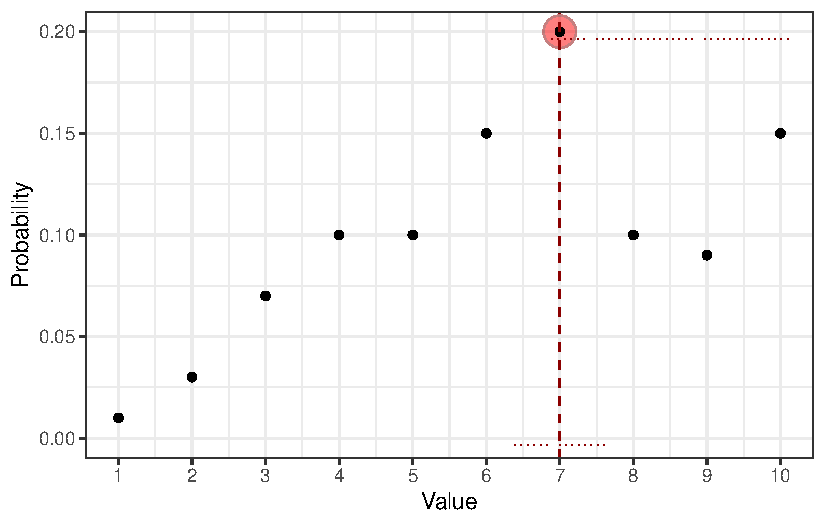
\includegraphics{andan-descriptives_files/figure-pdf/fig-mode-pmf-1.pdf}

}

\caption{\label{fig-mode-pmf}Определение моды с помощью функции
вероятности}

\end{figure}%

Окей, мы видим, что \emph{мода отлично считается на дискретных
переменных}. А как же быть с непрерывными?

\href{}{Напомним себе}, что вероятность того, что непрерывная случайная
величина примет своё конкретное значение, равна нулю. Из этого следует,
что все значения непрерывной случайное величины уникальны --- каждое
повторяется только один раз. Получается, что строить частотную таблицу
бессмысленно\ldots{}

По этой причине \textbf{для непрерывных переменных моду не считают}.

\subsubsection{Мода для непрерывной
переменной}\label{andan-descriptives-mode-contunious}

Да, это так. Действительно, посчитать моду для непрерывной переменной
способом, аналогичным тому, что мы увидели выше, не получится. Однако
математиков это не остановило.

Если мы посмотрим на \href{}{график плотности вероятности} (probability
density function, PDF), который является аналогом PMF для дискретных
переменных, мы увидим, что какие-то значения встречаются чаще, а
какие-то реже. Что в общем-то логично. Напомним себе, \href{}{как это
выглядит}, например, для любимого {[}стандартного{]} \href{}{нормального
распределения}:

\begin{verbatim}
Warning in grid.Call.graphics(C_text, as.graphicsAnnot(x$label), x$x, x$y, :
conversion failure on 'эти значения встречаются часто' in 'mbcsToSbcs': dot
substituted for <d1>
\end{verbatim}

\begin{verbatim}
Warning in grid.Call.graphics(C_text, as.graphicsAnnot(x$label), x$x, x$y, :
conversion failure on 'эти значения встречаются часто' in 'mbcsToSbcs': dot
substituted for <8d>
\end{verbatim}

\begin{verbatim}
Warning in grid.Call.graphics(C_text, as.graphicsAnnot(x$label), x$x, x$y, :
conversion failure on 'эти значения встречаются часто' in 'mbcsToSbcs': dot
substituted for <d1>
\end{verbatim}

\begin{verbatim}
Warning in grid.Call.graphics(C_text, as.graphicsAnnot(x$label), x$x, x$y, :
conversion failure on 'эти значения встречаются часто' in 'mbcsToSbcs': dot
substituted for <82>
\end{verbatim}

\begin{verbatim}
Warning in grid.Call.graphics(C_text, as.graphicsAnnot(x$label), x$x, x$y, :
conversion failure on 'эти значения встречаются часто' in 'mbcsToSbcs': dot
substituted for <d0>
\end{verbatim}

\begin{verbatim}
Warning in grid.Call.graphics(C_text, as.graphicsAnnot(x$label), x$x, x$y, :
conversion failure on 'эти значения встречаются часто' in 'mbcsToSbcs': dot
substituted for <b8>
\end{verbatim}

\begin{verbatim}
Warning in grid.Call.graphics(C_text, as.graphicsAnnot(x$label), x$x, x$y, :
conversion failure on 'эти значения встречаются часто' in 'mbcsToSbcs': dot
substituted for <d0>
\end{verbatim}

\begin{verbatim}
Warning in grid.Call.graphics(C_text, as.graphicsAnnot(x$label), x$x, x$y, :
conversion failure on 'эти значения встречаются часто' in 'mbcsToSbcs': dot
substituted for <b7>
\end{verbatim}

\begin{verbatim}
Warning in grid.Call.graphics(C_text, as.graphicsAnnot(x$label), x$x, x$y, :
conversion failure on 'эти значения встречаются часто' in 'mbcsToSbcs': dot
substituted for <d0>
\end{verbatim}

\begin{verbatim}
Warning in grid.Call.graphics(C_text, as.graphicsAnnot(x$label), x$x, x$y, :
conversion failure on 'эти значения встречаются часто' in 'mbcsToSbcs': dot
substituted for <bd>
\end{verbatim}

\begin{verbatim}
Warning in grid.Call.graphics(C_text, as.graphicsAnnot(x$label), x$x, x$y, :
conversion failure on 'эти значения встречаются часто' in 'mbcsToSbcs': dot
substituted for <d0>
\end{verbatim}

\begin{verbatim}
Warning in grid.Call.graphics(C_text, as.graphicsAnnot(x$label), x$x, x$y, :
conversion failure on 'эти значения встречаются часто' in 'mbcsToSbcs': dot
substituted for <b0>
\end{verbatim}

\begin{verbatim}
Warning in grid.Call.graphics(C_text, as.graphicsAnnot(x$label), x$x, x$y, :
conversion failure on 'эти значения встречаются часто' in 'mbcsToSbcs': dot
substituted for <d1>
\end{verbatim}

\begin{verbatim}
Warning in grid.Call.graphics(C_text, as.graphicsAnnot(x$label), x$x, x$y, :
conversion failure on 'эти значения встречаются часто' in 'mbcsToSbcs': dot
substituted for <87>
\end{verbatim}

\begin{verbatim}
Warning in grid.Call.graphics(C_text, as.graphicsAnnot(x$label), x$x, x$y, :
conversion failure on 'эти значения встречаются часто' in 'mbcsToSbcs': dot
substituted for <d0>
\end{verbatim}

\begin{verbatim}
Warning in grid.Call.graphics(C_text, as.graphicsAnnot(x$label), x$x, x$y, :
conversion failure on 'эти значения встречаются часто' in 'mbcsToSbcs': dot
substituted for <b5>
\end{verbatim}

\begin{verbatim}
Warning in grid.Call.graphics(C_text, as.graphicsAnnot(x$label), x$x, x$y, :
conversion failure on 'эти значения встречаются часто' in 'mbcsToSbcs': dot
substituted for <d0>
\end{verbatim}

\begin{verbatim}
Warning in grid.Call.graphics(C_text, as.graphicsAnnot(x$label), x$x, x$y, :
conversion failure on 'эти значения встречаются часто' in 'mbcsToSbcs': dot
substituted for <bd>
\end{verbatim}

\begin{verbatim}
Warning in grid.Call.graphics(C_text, as.graphicsAnnot(x$label), x$x, x$y, :
conversion failure on 'эти значения встречаются часто' in 'mbcsToSbcs': dot
substituted for <d0>
\end{verbatim}

\begin{verbatim}
Warning in grid.Call.graphics(C_text, as.graphicsAnnot(x$label), x$x, x$y, :
conversion failure on 'эти значения встречаются часто' in 'mbcsToSbcs': dot
substituted for <b8>
\end{verbatim}

\begin{verbatim}
Warning in grid.Call.graphics(C_text, as.graphicsAnnot(x$label), x$x, x$y, :
conversion failure on 'эти значения встречаются часто' in 'mbcsToSbcs': dot
substituted for <d1>
\end{verbatim}

\begin{verbatim}
Warning in grid.Call.graphics(C_text, as.graphicsAnnot(x$label), x$x, x$y, :
conversion failure on 'эти значения встречаются часто' in 'mbcsToSbcs': dot
substituted for <8f>
\end{verbatim}

\begin{verbatim}
Warning in grid.Call.graphics(C_text, as.graphicsAnnot(x$label), x$x, x$y, :
conversion failure on 'эти значения встречаются часто' in 'mbcsToSbcs': dot
substituted for <d0>
\end{verbatim}

\begin{verbatim}
Warning in grid.Call.graphics(C_text, as.graphicsAnnot(x$label), x$x, x$y, :
conversion failure on 'эти значения встречаются часто' in 'mbcsToSbcs': dot
substituted for <b2>
\end{verbatim}

\begin{verbatim}
Warning in grid.Call.graphics(C_text, as.graphicsAnnot(x$label), x$x, x$y, :
conversion failure on 'эти значения встречаются часто' in 'mbcsToSbcs': dot
substituted for <d1>
\end{verbatim}

\begin{verbatim}
Warning in grid.Call.graphics(C_text, as.graphicsAnnot(x$label), x$x, x$y, :
conversion failure on 'эти значения встречаются часто' in 'mbcsToSbcs': dot
substituted for <81>
\end{verbatim}

\begin{verbatim}
Warning in grid.Call.graphics(C_text, as.graphicsAnnot(x$label), x$x, x$y, :
conversion failure on 'эти значения встречаются часто' in 'mbcsToSbcs': dot
substituted for <d1>
\end{verbatim}

\begin{verbatim}
Warning in grid.Call.graphics(C_text, as.graphicsAnnot(x$label), x$x, x$y, :
conversion failure on 'эти значения встречаются часто' in 'mbcsToSbcs': dot
substituted for <82>
\end{verbatim}

\begin{verbatim}
Warning in grid.Call.graphics(C_text, as.graphicsAnnot(x$label), x$x, x$y, :
conversion failure on 'эти значения встречаются часто' in 'mbcsToSbcs': dot
substituted for <d1>
\end{verbatim}

\begin{verbatim}
Warning in grid.Call.graphics(C_text, as.graphicsAnnot(x$label), x$x, x$y, :
conversion failure on 'эти значения встречаются часто' in 'mbcsToSbcs': dot
substituted for <80>
\end{verbatim}

\begin{verbatim}
Warning in grid.Call.graphics(C_text, as.graphicsAnnot(x$label), x$x, x$y, :
conversion failure on 'эти значения встречаются часто' in 'mbcsToSbcs': dot
substituted for <d0>
\end{verbatim}

\begin{verbatim}
Warning in grid.Call.graphics(C_text, as.graphicsAnnot(x$label), x$x, x$y, :
conversion failure on 'эти значения встречаются часто' in 'mbcsToSbcs': dot
substituted for <b5>
\end{verbatim}

\begin{verbatim}
Warning in grid.Call.graphics(C_text, as.graphicsAnnot(x$label), x$x, x$y, :
conversion failure on 'эти значения встречаются часто' in 'mbcsToSbcs': dot
substituted for <d1>
\end{verbatim}

\begin{verbatim}
Warning in grid.Call.graphics(C_text, as.graphicsAnnot(x$label), x$x, x$y, :
conversion failure on 'эти значения встречаются часто' in 'mbcsToSbcs': dot
substituted for <87>
\end{verbatim}

\begin{verbatim}
Warning in grid.Call.graphics(C_text, as.graphicsAnnot(x$label), x$x, x$y, :
conversion failure on 'эти значения встречаются часто' in 'mbcsToSbcs': dot
substituted for <d0>
\end{verbatim}

\begin{verbatim}
Warning in grid.Call.graphics(C_text, as.graphicsAnnot(x$label), x$x, x$y, :
conversion failure on 'эти значения встречаются часто' in 'mbcsToSbcs': dot
substituted for <b0>
\end{verbatim}

\begin{verbatim}
Warning in grid.Call.graphics(C_text, as.graphicsAnnot(x$label), x$x, x$y, :
conversion failure on 'эти значения встречаются часто' in 'mbcsToSbcs': dot
substituted for <d1>
\end{verbatim}

\begin{verbatim}
Warning in grid.Call.graphics(C_text, as.graphicsAnnot(x$label), x$x, x$y, :
conversion failure on 'эти значения встречаются часто' in 'mbcsToSbcs': dot
substituted for <8e>
\end{verbatim}

\begin{verbatim}
Warning in grid.Call.graphics(C_text, as.graphicsAnnot(x$label), x$x, x$y, :
conversion failure on 'эти значения встречаются часто' in 'mbcsToSbcs': dot
substituted for <d1>
\end{verbatim}

\begin{verbatim}
Warning in grid.Call.graphics(C_text, as.graphicsAnnot(x$label), x$x, x$y, :
conversion failure on 'эти значения встречаются часто' in 'mbcsToSbcs': dot
substituted for <82>
\end{verbatim}

\begin{verbatim}
Warning in grid.Call.graphics(C_text, as.graphicsAnnot(x$label), x$x, x$y, :
conversion failure on 'эти значения встречаются часто' in 'mbcsToSbcs': dot
substituted for <d1>
\end{verbatim}

\begin{verbatim}
Warning in grid.Call.graphics(C_text, as.graphicsAnnot(x$label), x$x, x$y, :
conversion failure on 'эти значения встречаются часто' in 'mbcsToSbcs': dot
substituted for <81>
\end{verbatim}

\begin{verbatim}
Warning in grid.Call.graphics(C_text, as.graphicsAnnot(x$label), x$x, x$y, :
conversion failure on 'эти значения встречаются часто' in 'mbcsToSbcs': dot
substituted for <d1>
\end{verbatim}

\begin{verbatim}
Warning in grid.Call.graphics(C_text, as.graphicsAnnot(x$label), x$x, x$y, :
conversion failure on 'эти значения встречаются часто' in 'mbcsToSbcs': dot
substituted for <8f>
\end{verbatim}

\begin{verbatim}
Warning in grid.Call.graphics(C_text, as.graphicsAnnot(x$label), x$x, x$y, :
conversion failure on 'эти значения встречаются часто' in 'mbcsToSbcs': dot
substituted for <d1>
\end{verbatim}

\begin{verbatim}
Warning in grid.Call.graphics(C_text, as.graphicsAnnot(x$label), x$x, x$y, :
conversion failure on 'эти значения встречаются часто' in 'mbcsToSbcs': dot
substituted for <87>
\end{verbatim}

\begin{verbatim}
Warning in grid.Call.graphics(C_text, as.graphicsAnnot(x$label), x$x, x$y, :
conversion failure on 'эти значения встречаются часто' in 'mbcsToSbcs': dot
substituted for <d0>
\end{verbatim}

\begin{verbatim}
Warning in grid.Call.graphics(C_text, as.graphicsAnnot(x$label), x$x, x$y, :
conversion failure on 'эти значения встречаются часто' in 'mbcsToSbcs': dot
substituted for <b0>
\end{verbatim}

\begin{verbatim}
Warning in grid.Call.graphics(C_text, as.graphicsAnnot(x$label), x$x, x$y, :
conversion failure on 'эти значения встречаются часто' in 'mbcsToSbcs': dot
substituted for <d1>
\end{verbatim}

\begin{verbatim}
Warning in grid.Call.graphics(C_text, as.graphicsAnnot(x$label), x$x, x$y, :
conversion failure on 'эти значения встречаются часто' in 'mbcsToSbcs': dot
substituted for <81>
\end{verbatim}

\begin{verbatim}
Warning in grid.Call.graphics(C_text, as.graphicsAnnot(x$label), x$x, x$y, :
conversion failure on 'эти значения встречаются часто' in 'mbcsToSbcs': dot
substituted for <d1>
\end{verbatim}

\begin{verbatim}
Warning in grid.Call.graphics(C_text, as.graphicsAnnot(x$label), x$x, x$y, :
conversion failure on 'эти значения встречаются часто' in 'mbcsToSbcs': dot
substituted for <82>
\end{verbatim}

\begin{verbatim}
Warning in grid.Call.graphics(C_text, as.graphicsAnnot(x$label), x$x, x$y, :
conversion failure on 'эти значения встречаются часто' in 'mbcsToSbcs': dot
substituted for <d0>
\end{verbatim}

\begin{verbatim}
Warning in grid.Call.graphics(C_text, as.graphicsAnnot(x$label), x$x, x$y, :
conversion failure on 'эти значения встречаются часто' in 'mbcsToSbcs': dot
substituted for <be>
\end{verbatim}

\begin{verbatim}
Warning in grid.Call.graphics(C_text, as.graphicsAnnot(x$label), x$x, x$y, :
conversion failure on 'эти значения' in 'mbcsToSbcs': dot substituted for <d1>
\end{verbatim}

\begin{verbatim}
Warning in grid.Call.graphics(C_text, as.graphicsAnnot(x$label), x$x, x$y, :
conversion failure on 'эти значения' in 'mbcsToSbcs': dot substituted for <8d>
\end{verbatim}

\begin{verbatim}
Warning in grid.Call.graphics(C_text, as.graphicsAnnot(x$label), x$x, x$y, :
conversion failure on 'эти значения' in 'mbcsToSbcs': dot substituted for <d1>
\end{verbatim}

\begin{verbatim}
Warning in grid.Call.graphics(C_text, as.graphicsAnnot(x$label), x$x, x$y, :
conversion failure on 'эти значения' in 'mbcsToSbcs': dot substituted for <82>
\end{verbatim}

\begin{verbatim}
Warning in grid.Call.graphics(C_text, as.graphicsAnnot(x$label), x$x, x$y, :
conversion failure on 'эти значения' in 'mbcsToSbcs': dot substituted for <d0>
\end{verbatim}

\begin{verbatim}
Warning in grid.Call.graphics(C_text, as.graphicsAnnot(x$label), x$x, x$y, :
conversion failure on 'эти значения' in 'mbcsToSbcs': dot substituted for <b8>
\end{verbatim}

\begin{verbatim}
Warning in grid.Call.graphics(C_text, as.graphicsAnnot(x$label), x$x, x$y, :
conversion failure on 'эти значения' in 'mbcsToSbcs': dot substituted for <d0>
\end{verbatim}

\begin{verbatim}
Warning in grid.Call.graphics(C_text, as.graphicsAnnot(x$label), x$x, x$y, :
conversion failure on 'эти значения' in 'mbcsToSbcs': dot substituted for <b7>
\end{verbatim}

\begin{verbatim}
Warning in grid.Call.graphics(C_text, as.graphicsAnnot(x$label), x$x, x$y, :
conversion failure on 'эти значения' in 'mbcsToSbcs': dot substituted for <d0>
\end{verbatim}

\begin{verbatim}
Warning in grid.Call.graphics(C_text, as.graphicsAnnot(x$label), x$x, x$y, :
conversion failure on 'эти значения' in 'mbcsToSbcs': dot substituted for <bd>
\end{verbatim}

\begin{verbatim}
Warning in grid.Call.graphics(C_text, as.graphicsAnnot(x$label), x$x, x$y, :
conversion failure on 'эти значения' in 'mbcsToSbcs': dot substituted for <d0>
\end{verbatim}

\begin{verbatim}
Warning in grid.Call.graphics(C_text, as.graphicsAnnot(x$label), x$x, x$y, :
conversion failure on 'эти значения' in 'mbcsToSbcs': dot substituted for <b0>
\end{verbatim}

\begin{verbatim}
Warning in grid.Call.graphics(C_text, as.graphicsAnnot(x$label), x$x, x$y, :
conversion failure on 'эти значения' in 'mbcsToSbcs': dot substituted for <d1>
\end{verbatim}

\begin{verbatim}
Warning in grid.Call.graphics(C_text, as.graphicsAnnot(x$label), x$x, x$y, :
conversion failure on 'эти значения' in 'mbcsToSbcs': dot substituted for <87>
\end{verbatim}

\begin{verbatim}
Warning in grid.Call.graphics(C_text, as.graphicsAnnot(x$label), x$x, x$y, :
conversion failure on 'эти значения' in 'mbcsToSbcs': dot substituted for <d0>
\end{verbatim}

\begin{verbatim}
Warning in grid.Call.graphics(C_text, as.graphicsAnnot(x$label), x$x, x$y, :
conversion failure on 'эти значения' in 'mbcsToSbcs': dot substituted for <b5>
\end{verbatim}

\begin{verbatim}
Warning in grid.Call.graphics(C_text, as.graphicsAnnot(x$label), x$x, x$y, :
conversion failure on 'эти значения' in 'mbcsToSbcs': dot substituted for <d0>
\end{verbatim}

\begin{verbatim}
Warning in grid.Call.graphics(C_text, as.graphicsAnnot(x$label), x$x, x$y, :
conversion failure on 'эти значения' in 'mbcsToSbcs': dot substituted for <bd>
\end{verbatim}

\begin{verbatim}
Warning in grid.Call.graphics(C_text, as.graphicsAnnot(x$label), x$x, x$y, :
conversion failure on 'эти значения' in 'mbcsToSbcs': dot substituted for <d0>
\end{verbatim}

\begin{verbatim}
Warning in grid.Call.graphics(C_text, as.graphicsAnnot(x$label), x$x, x$y, :
conversion failure on 'эти значения' in 'mbcsToSbcs': dot substituted for <b8>
\end{verbatim}

\begin{verbatim}
Warning in grid.Call.graphics(C_text, as.graphicsAnnot(x$label), x$x, x$y, :
conversion failure on 'эти значения' in 'mbcsToSbcs': dot substituted for <d1>
\end{verbatim}

\begin{verbatim}
Warning in grid.Call.graphics(C_text, as.graphicsAnnot(x$label), x$x, x$y, :
conversion failure on 'эти значения' in 'mbcsToSbcs': dot substituted for <8f>
\end{verbatim}

\begin{verbatim}
Warning in grid.Call.graphics(C_text, as.graphicsAnnot(x$label), x$x, x$y, :
conversion failure on 'встречаются реже' in 'mbcsToSbcs': dot substituted for
<d0>
\end{verbatim}

\begin{verbatim}
Warning in grid.Call.graphics(C_text, as.graphicsAnnot(x$label), x$x, x$y, :
conversion failure on 'встречаются реже' in 'mbcsToSbcs': dot substituted for
<b2>
\end{verbatim}

\begin{verbatim}
Warning in grid.Call.graphics(C_text, as.graphicsAnnot(x$label), x$x, x$y, :
conversion failure on 'встречаются реже' in 'mbcsToSbcs': dot substituted for
<d1>
\end{verbatim}

\begin{verbatim}
Warning in grid.Call.graphics(C_text, as.graphicsAnnot(x$label), x$x, x$y, :
conversion failure on 'встречаются реже' in 'mbcsToSbcs': dot substituted for
<81>
\end{verbatim}

\begin{verbatim}
Warning in grid.Call.graphics(C_text, as.graphicsAnnot(x$label), x$x, x$y, :
conversion failure on 'встречаются реже' in 'mbcsToSbcs': dot substituted for
<d1>
\end{verbatim}

\begin{verbatim}
Warning in grid.Call.graphics(C_text, as.graphicsAnnot(x$label), x$x, x$y, :
conversion failure on 'встречаются реже' in 'mbcsToSbcs': dot substituted for
<82>
\end{verbatim}

\begin{verbatim}
Warning in grid.Call.graphics(C_text, as.graphicsAnnot(x$label), x$x, x$y, :
conversion failure on 'встречаются реже' in 'mbcsToSbcs': dot substituted for
<d1>
\end{verbatim}

\begin{verbatim}
Warning in grid.Call.graphics(C_text, as.graphicsAnnot(x$label), x$x, x$y, :
conversion failure on 'встречаются реже' in 'mbcsToSbcs': dot substituted for
<80>
\end{verbatim}

\begin{verbatim}
Warning in grid.Call.graphics(C_text, as.graphicsAnnot(x$label), x$x, x$y, :
conversion failure on 'встречаются реже' in 'mbcsToSbcs': dot substituted for
<d0>
\end{verbatim}

\begin{verbatim}
Warning in grid.Call.graphics(C_text, as.graphicsAnnot(x$label), x$x, x$y, :
conversion failure on 'встречаются реже' in 'mbcsToSbcs': dot substituted for
<b5>
\end{verbatim}

\begin{verbatim}
Warning in grid.Call.graphics(C_text, as.graphicsAnnot(x$label), x$x, x$y, :
conversion failure on 'встречаются реже' in 'mbcsToSbcs': dot substituted for
<d1>
\end{verbatim}

\begin{verbatim}
Warning in grid.Call.graphics(C_text, as.graphicsAnnot(x$label), x$x, x$y, :
conversion failure on 'встречаются реже' in 'mbcsToSbcs': dot substituted for
<87>
\end{verbatim}

\begin{verbatim}
Warning in grid.Call.graphics(C_text, as.graphicsAnnot(x$label), x$x, x$y, :
conversion failure on 'встречаются реже' in 'mbcsToSbcs': dot substituted for
<d0>
\end{verbatim}

\begin{verbatim}
Warning in grid.Call.graphics(C_text, as.graphicsAnnot(x$label), x$x, x$y, :
conversion failure on 'встречаются реже' in 'mbcsToSbcs': dot substituted for
<b0>
\end{verbatim}

\begin{verbatim}
Warning in grid.Call.graphics(C_text, as.graphicsAnnot(x$label), x$x, x$y, :
conversion failure on 'встречаются реже' in 'mbcsToSbcs': dot substituted for
<d1>
\end{verbatim}

\begin{verbatim}
Warning in grid.Call.graphics(C_text, as.graphicsAnnot(x$label), x$x, x$y, :
conversion failure on 'встречаются реже' in 'mbcsToSbcs': dot substituted for
<8e>
\end{verbatim}

\begin{verbatim}
Warning in grid.Call.graphics(C_text, as.graphicsAnnot(x$label), x$x, x$y, :
conversion failure on 'встречаются реже' in 'mbcsToSbcs': dot substituted for
<d1>
\end{verbatim}

\begin{verbatim}
Warning in grid.Call.graphics(C_text, as.graphicsAnnot(x$label), x$x, x$y, :
conversion failure on 'встречаются реже' in 'mbcsToSbcs': dot substituted for
<82>
\end{verbatim}

\begin{verbatim}
Warning in grid.Call.graphics(C_text, as.graphicsAnnot(x$label), x$x, x$y, :
conversion failure on 'встречаются реже' in 'mbcsToSbcs': dot substituted for
<d1>
\end{verbatim}

\begin{verbatim}
Warning in grid.Call.graphics(C_text, as.graphicsAnnot(x$label), x$x, x$y, :
conversion failure on 'встречаются реже' in 'mbcsToSbcs': dot substituted for
<81>
\end{verbatim}

\begin{verbatim}
Warning in grid.Call.graphics(C_text, as.graphicsAnnot(x$label), x$x, x$y, :
conversion failure on 'встречаются реже' in 'mbcsToSbcs': dot substituted for
<d1>
\end{verbatim}

\begin{verbatim}
Warning in grid.Call.graphics(C_text, as.graphicsAnnot(x$label), x$x, x$y, :
conversion failure on 'встречаются реже' in 'mbcsToSbcs': dot substituted for
<8f>
\end{verbatim}

\begin{verbatim}
Warning in grid.Call.graphics(C_text, as.graphicsAnnot(x$label), x$x, x$y, :
conversion failure on 'встречаются реже' in 'mbcsToSbcs': dot substituted for
<d1>
\end{verbatim}

\begin{verbatim}
Warning in grid.Call.graphics(C_text, as.graphicsAnnot(x$label), x$x, x$y, :
conversion failure on 'встречаются реже' in 'mbcsToSbcs': dot substituted for
<80>
\end{verbatim}

\begin{verbatim}
Warning in grid.Call.graphics(C_text, as.graphicsAnnot(x$label), x$x, x$y, :
conversion failure on 'встречаются реже' in 'mbcsToSbcs': dot substituted for
<d0>
\end{verbatim}

\begin{verbatim}
Warning in grid.Call.graphics(C_text, as.graphicsAnnot(x$label), x$x, x$y, :
conversion failure on 'встречаются реже' in 'mbcsToSbcs': dot substituted for
<b5>
\end{verbatim}

\begin{verbatim}
Warning in grid.Call.graphics(C_text, as.graphicsAnnot(x$label), x$x, x$y, :
conversion failure on 'встречаются реже' in 'mbcsToSbcs': dot substituted for
<d0>
\end{verbatim}

\begin{verbatim}
Warning in grid.Call.graphics(C_text, as.graphicsAnnot(x$label), x$x, x$y, :
conversion failure on 'встречаются реже' in 'mbcsToSbcs': dot substituted for
<b6>
\end{verbatim}

\begin{verbatim}
Warning in grid.Call.graphics(C_text, as.graphicsAnnot(x$label), x$x, x$y, :
conversion failure on 'встречаются реже' in 'mbcsToSbcs': dot substituted for
<d0>
\end{verbatim}

\begin{verbatim}
Warning in grid.Call.graphics(C_text, as.graphicsAnnot(x$label), x$x, x$y, :
conversion failure on 'встречаются реже' in 'mbcsToSbcs': dot substituted for
<b5>
\end{verbatim}

\begin{figure}

\centering{

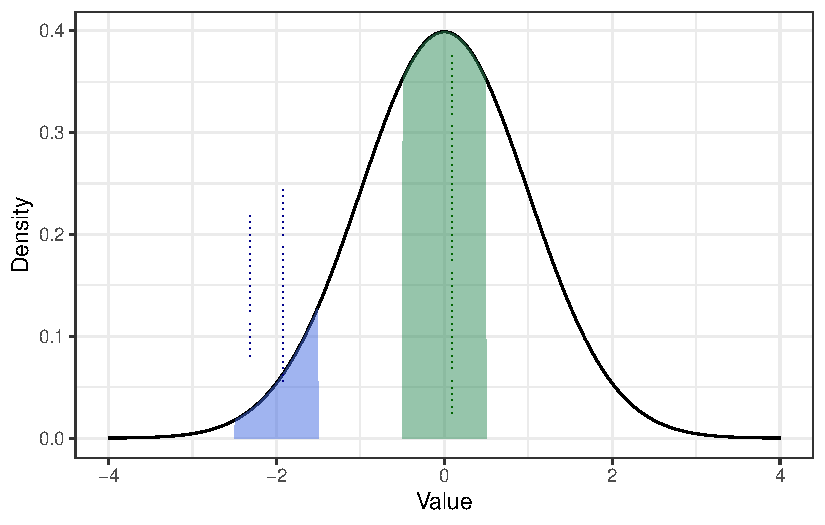
\includegraphics{andan-descriptives_files/figure-pdf/fig-continuous-freqs-1.pdf}

}

\caption{\label{fig-continuous-freqs}Частоты интервалов значений
непрерывной случайной величины на функции плотности распределения}

\end{figure}%

То есть, самые часто встречающиеся значения --- это \textbf{пик
распределения}. Там и должна быть мода. Визуально это выглядит
достаточно справедливо.

Математики так и решили:

\begin{definition}[]\protect\hypertarget{def-mode-continuous}{}\label{def-mode-continuous}

\textbf{Мода} {[}непрерывной переменной{]} --- это значение переменной,
при котором её функция плотности вероятности достигает
локального\footnote{Здесь в примере локальный максимум функции плотности
  вероятности на интервале \((-4, \, 4)\) совпадает с глобальным
  максимумом --- мы об этом знаем, потому что форма распределения нам
  известна. В случае эмпрического распределения корректнее говорить
  именно о локальном максимуме, так как глобальный максимум нам не
  доступен ввиду того, что мы работаем с выборкой.} максимума.

\end{definition}

\begin{equation}\phantomsection\label{eq-mode-pdf}{
\text{mode}(X) = \arg \max(\text{PDF}(X)) = \arg \max_{x \in S}f(x),
}\end{equation}

гдe \(X\) --- непрерывная случайная величина, \(x\) --- значение этой
случайной величины, \(S\) --- имеющаяся выборка значений переменной.

\begin{verbatim}
Warning in grid.Call.graphics(C_text, as.graphicsAnnot(x$label), x$x, x$y, :
conversion failure on 'мода тут' in 'mbcsToSbcs': dot substituted for <d0>
\end{verbatim}

\begin{verbatim}
Warning in grid.Call.graphics(C_text, as.graphicsAnnot(x$label), x$x, x$y, :
conversion failure on 'мода тут' in 'mbcsToSbcs': dot substituted for <bc>
\end{verbatim}

\begin{verbatim}
Warning in grid.Call.graphics(C_text, as.graphicsAnnot(x$label), x$x, x$y, :
conversion failure on 'мода тут' in 'mbcsToSbcs': dot substituted for <d0>
\end{verbatim}

\begin{verbatim}
Warning in grid.Call.graphics(C_text, as.graphicsAnnot(x$label), x$x, x$y, :
conversion failure on 'мода тут' in 'mbcsToSbcs': dot substituted for <be>
\end{verbatim}

\begin{verbatim}
Warning in grid.Call.graphics(C_text, as.graphicsAnnot(x$label), x$x, x$y, :
conversion failure on 'мода тут' in 'mbcsToSbcs': dot substituted for <d0>
\end{verbatim}

\begin{verbatim}
Warning in grid.Call.graphics(C_text, as.graphicsAnnot(x$label), x$x, x$y, :
conversion failure on 'мода тут' in 'mbcsToSbcs': dot substituted for <b4>
\end{verbatim}

\begin{verbatim}
Warning in grid.Call.graphics(C_text, as.graphicsAnnot(x$label), x$x, x$y, :
conversion failure on 'мода тут' in 'mbcsToSbcs': dot substituted for <d0>
\end{verbatim}

\begin{verbatim}
Warning in grid.Call.graphics(C_text, as.graphicsAnnot(x$label), x$x, x$y, :
conversion failure on 'мода тут' in 'mbcsToSbcs': dot substituted for <b0>
\end{verbatim}

\begin{verbatim}
Warning in grid.Call.graphics(C_text, as.graphicsAnnot(x$label), x$x, x$y, :
conversion failure on 'мода тут' in 'mbcsToSbcs': dot substituted for <d1>
\end{verbatim}

\begin{verbatim}
Warning in grid.Call.graphics(C_text, as.graphicsAnnot(x$label), x$x, x$y, :
conversion failure on 'мода тут' in 'mbcsToSbcs': dot substituted for <82>
\end{verbatim}

\begin{verbatim}
Warning in grid.Call.graphics(C_text, as.graphicsAnnot(x$label), x$x, x$y, :
conversion failure on 'мода тут' in 'mbcsToSbcs': dot substituted for <d1>
\end{verbatim}

\begin{verbatim}
Warning in grid.Call.graphics(C_text, as.graphicsAnnot(x$label), x$x, x$y, :
conversion failure on 'мода тут' in 'mbcsToSbcs': dot substituted for <83>
\end{verbatim}

\begin{verbatim}
Warning in grid.Call.graphics(C_text, as.graphicsAnnot(x$label), x$x, x$y, :
conversion failure on 'мода тут' in 'mbcsToSbcs': dot substituted for <d1>
\end{verbatim}

\begin{verbatim}
Warning in grid.Call.graphics(C_text, as.graphicsAnnot(x$label), x$x, x$y, :
conversion failure on 'мода тут' in 'mbcsToSbcs': dot substituted for <82>
\end{verbatim}

\begin{verbatim}
Warning in grid.Call.graphics(C_text, as.graphicsAnnot(x$label), x$x, x$y, :
conversion failure on 'локальный максимум тут' in 'mbcsToSbcs': dot substituted
for <d0>
\end{verbatim}

\begin{verbatim}
Warning in grid.Call.graphics(C_text, as.graphicsAnnot(x$label), x$x, x$y, :
conversion failure on 'локальный максимум тут' in 'mbcsToSbcs': dot substituted
for <bb>
\end{verbatim}

\begin{verbatim}
Warning in grid.Call.graphics(C_text, as.graphicsAnnot(x$label), x$x, x$y, :
conversion failure on 'локальный максимум тут' in 'mbcsToSbcs': dot substituted
for <d0>
\end{verbatim}

\begin{verbatim}
Warning in grid.Call.graphics(C_text, as.graphicsAnnot(x$label), x$x, x$y, :
conversion failure on 'локальный максимум тут' in 'mbcsToSbcs': dot substituted
for <be>
\end{verbatim}

\begin{verbatim}
Warning in grid.Call.graphics(C_text, as.graphicsAnnot(x$label), x$x, x$y, :
conversion failure on 'локальный максимум тут' in 'mbcsToSbcs': dot substituted
for <d0>
\end{verbatim}

\begin{verbatim}
Warning in grid.Call.graphics(C_text, as.graphicsAnnot(x$label), x$x, x$y, :
conversion failure on 'локальный максимум тут' in 'mbcsToSbcs': dot substituted
for <ba>
\end{verbatim}

\begin{verbatim}
Warning in grid.Call.graphics(C_text, as.graphicsAnnot(x$label), x$x, x$y, :
conversion failure on 'локальный максимум тут' in 'mbcsToSbcs': dot substituted
for <d0>
\end{verbatim}

\begin{verbatim}
Warning in grid.Call.graphics(C_text, as.graphicsAnnot(x$label), x$x, x$y, :
conversion failure on 'локальный максимум тут' in 'mbcsToSbcs': dot substituted
for <b0>
\end{verbatim}

\begin{verbatim}
Warning in grid.Call.graphics(C_text, as.graphicsAnnot(x$label), x$x, x$y, :
conversion failure on 'локальный максимум тут' in 'mbcsToSbcs': dot substituted
for <d0>
\end{verbatim}

\begin{verbatim}
Warning in grid.Call.graphics(C_text, as.graphicsAnnot(x$label), x$x, x$y, :
conversion failure on 'локальный максимум тут' in 'mbcsToSbcs': dot substituted
for <bb>
\end{verbatim}

\begin{verbatim}
Warning in grid.Call.graphics(C_text, as.graphicsAnnot(x$label), x$x, x$y, :
conversion failure on 'локальный максимум тут' in 'mbcsToSbcs': dot substituted
for <d1>
\end{verbatim}

\begin{verbatim}
Warning in grid.Call.graphics(C_text, as.graphicsAnnot(x$label), x$x, x$y, :
conversion failure on 'локальный максимум тут' in 'mbcsToSbcs': dot substituted
for <8c>
\end{verbatim}

\begin{verbatim}
Warning in grid.Call.graphics(C_text, as.graphicsAnnot(x$label), x$x, x$y, :
conversion failure on 'локальный максимум тут' in 'mbcsToSbcs': dot substituted
for <d0>
\end{verbatim}

\begin{verbatim}
Warning in grid.Call.graphics(C_text, as.graphicsAnnot(x$label), x$x, x$y, :
conversion failure on 'локальный максимум тут' in 'mbcsToSbcs': dot substituted
for <bd>
\end{verbatim}

\begin{verbatim}
Warning in grid.Call.graphics(C_text, as.graphicsAnnot(x$label), x$x, x$y, :
conversion failure on 'локальный максимум тут' in 'mbcsToSbcs': dot substituted
for <d1>
\end{verbatim}

\begin{verbatim}
Warning in grid.Call.graphics(C_text, as.graphicsAnnot(x$label), x$x, x$y, :
conversion failure on 'локальный максимум тут' in 'mbcsToSbcs': dot substituted
for <8b>
\end{verbatim}

\begin{verbatim}
Warning in grid.Call.graphics(C_text, as.graphicsAnnot(x$label), x$x, x$y, :
conversion failure on 'локальный максимум тут' in 'mbcsToSbcs': dot substituted
for <d0>
\end{verbatim}

\begin{verbatim}
Warning in grid.Call.graphics(C_text, as.graphicsAnnot(x$label), x$x, x$y, :
conversion failure on 'локальный максимум тут' in 'mbcsToSbcs': dot substituted
for <b9>
\end{verbatim}

\begin{verbatim}
Warning in grid.Call.graphics(C_text, as.graphicsAnnot(x$label), x$x, x$y, :
conversion failure on 'локальный максимум тут' in 'mbcsToSbcs': dot substituted
for <d0>
\end{verbatim}

\begin{verbatim}
Warning in grid.Call.graphics(C_text, as.graphicsAnnot(x$label), x$x, x$y, :
conversion failure on 'локальный максимум тут' in 'mbcsToSbcs': dot substituted
for <bc>
\end{verbatim}

\begin{verbatim}
Warning in grid.Call.graphics(C_text, as.graphicsAnnot(x$label), x$x, x$y, :
conversion failure on 'локальный максимум тут' in 'mbcsToSbcs': dot substituted
for <d0>
\end{verbatim}

\begin{verbatim}
Warning in grid.Call.graphics(C_text, as.graphicsAnnot(x$label), x$x, x$y, :
conversion failure on 'локальный максимум тут' in 'mbcsToSbcs': dot substituted
for <b0>
\end{verbatim}

\begin{verbatim}
Warning in grid.Call.graphics(C_text, as.graphicsAnnot(x$label), x$x, x$y, :
conversion failure on 'локальный максимум тут' in 'mbcsToSbcs': dot substituted
for <d0>
\end{verbatim}

\begin{verbatim}
Warning in grid.Call.graphics(C_text, as.graphicsAnnot(x$label), x$x, x$y, :
conversion failure on 'локальный максимум тут' in 'mbcsToSbcs': dot substituted
for <ba>
\end{verbatim}

\begin{verbatim}
Warning in grid.Call.graphics(C_text, as.graphicsAnnot(x$label), x$x, x$y, :
conversion failure on 'локальный максимум тут' in 'mbcsToSbcs': dot substituted
for <d1>
\end{verbatim}

\begin{verbatim}
Warning in grid.Call.graphics(C_text, as.graphicsAnnot(x$label), x$x, x$y, :
conversion failure on 'локальный максимум тут' in 'mbcsToSbcs': dot substituted
for <81>
\end{verbatim}

\begin{verbatim}
Warning in grid.Call.graphics(C_text, as.graphicsAnnot(x$label), x$x, x$y, :
conversion failure on 'локальный максимум тут' in 'mbcsToSbcs': dot substituted
for <d0>
\end{verbatim}

\begin{verbatim}
Warning in grid.Call.graphics(C_text, as.graphicsAnnot(x$label), x$x, x$y, :
conversion failure on 'локальный максимум тут' in 'mbcsToSbcs': dot substituted
for <b8>
\end{verbatim}

\begin{verbatim}
Warning in grid.Call.graphics(C_text, as.graphicsAnnot(x$label), x$x, x$y, :
conversion failure on 'локальный максимум тут' in 'mbcsToSbcs': dot substituted
for <d0>
\end{verbatim}

\begin{verbatim}
Warning in grid.Call.graphics(C_text, as.graphicsAnnot(x$label), x$x, x$y, :
conversion failure on 'локальный максимум тут' in 'mbcsToSbcs': dot substituted
for <bc>
\end{verbatim}

\begin{verbatim}
Warning in grid.Call.graphics(C_text, as.graphicsAnnot(x$label), x$x, x$y, :
conversion failure on 'локальный максимум тут' in 'mbcsToSbcs': dot substituted
for <d1>
\end{verbatim}

\begin{verbatim}
Warning in grid.Call.graphics(C_text, as.graphicsAnnot(x$label), x$x, x$y, :
conversion failure on 'локальный максимум тут' in 'mbcsToSbcs': dot substituted
for <83>
\end{verbatim}

\begin{verbatim}
Warning in grid.Call.graphics(C_text, as.graphicsAnnot(x$label), x$x, x$y, :
conversion failure on 'локальный максимум тут' in 'mbcsToSbcs': dot substituted
for <d0>
\end{verbatim}

\begin{verbatim}
Warning in grid.Call.graphics(C_text, as.graphicsAnnot(x$label), x$x, x$y, :
conversion failure on 'локальный максимум тут' in 'mbcsToSbcs': dot substituted
for <bc>
\end{verbatim}

\begin{verbatim}
Warning in grid.Call.graphics(C_text, as.graphicsAnnot(x$label), x$x, x$y, :
conversion failure on 'локальный максимум тут' in 'mbcsToSbcs': dot substituted
for <d1>
\end{verbatim}

\begin{verbatim}
Warning in grid.Call.graphics(C_text, as.graphicsAnnot(x$label), x$x, x$y, :
conversion failure on 'локальный максимум тут' in 'mbcsToSbcs': dot substituted
for <82>
\end{verbatim}

\begin{verbatim}
Warning in grid.Call.graphics(C_text, as.graphicsAnnot(x$label), x$x, x$y, :
conversion failure on 'локальный максимум тут' in 'mbcsToSbcs': dot substituted
for <d1>
\end{verbatim}

\begin{verbatim}
Warning in grid.Call.graphics(C_text, as.graphicsAnnot(x$label), x$x, x$y, :
conversion failure on 'локальный максимум тут' in 'mbcsToSbcs': dot substituted
for <83>
\end{verbatim}

\begin{verbatim}
Warning in grid.Call.graphics(C_text, as.graphicsAnnot(x$label), x$x, x$y, :
conversion failure on 'локальный максимум тут' in 'mbcsToSbcs': dot substituted
for <d1>
\end{verbatim}

\begin{verbatim}
Warning in grid.Call.graphics(C_text, as.graphicsAnnot(x$label), x$x, x$y, :
conversion failure on 'локальный максимум тут' in 'mbcsToSbcs': dot substituted
for <82>
\end{verbatim}

\begin{figure}

\centering{

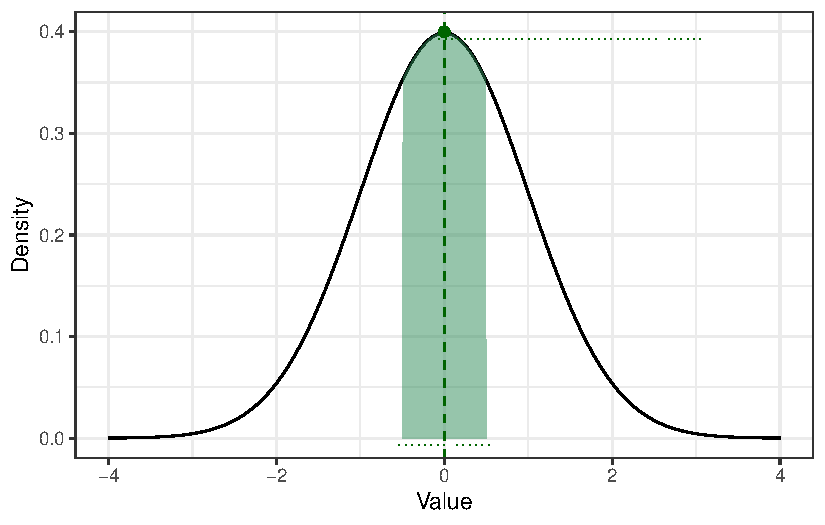
\includegraphics{andan-descriptives_files/figure-pdf/fig-continuous-mode-1.pdf}

}

\caption{\label{fig-continuous-mode}Положение моды на функции плотности
{[}стандартного{]} нормального распределения}

\end{figure}%

Хотя моду для непрерывной переменной вычислить можно, обычно этого не
делают, так как достаточно других мер центральной тенденции для описания
распределения.

\begin{center}\rule{0.5\linewidth}{0.5pt}\end{center}

\begin{tcolorbox}[enhanced jigsaw, colback=white, bottomrule=.15mm, opacityback=0, opacitybacktitle=0.6, breakable, coltitle=black, colframe=quarto-callout-warning-color-frame, titlerule=0mm, rightrule=.15mm, bottomtitle=1mm, leftrule=.75mm, toptitle=1mm, left=2mm, arc=.35mm, title=\textcolor{quarto-callout-warning-color}{\faExclamationTriangle}\hspace{0.5em}{Take-home: мода}, colbacktitle=quarto-callout-warning-color!10!white, toprule=.15mm]

\begin{itemize}
\tightlist
\item
  мода --- это значение переменной, которое встречается в выборке чаще
  всего
\item
  на практике она рассчитывается через построение частотной таблицы
\item
  используется с дискретными (номинальными и порядковыми) переменными
\item
  для непрерывных переменных её рассчитать можно, но обычного этого не
  делают
\end{itemize}

\end{tcolorbox}

\subsection{Унимодальные и полимодальные
распределения}\label{andan-descriptives-unimodal-bimodal}

Нормальное распределение, как и ряд других --- биномиальное,
отрицательное биномиальное, пуассоновское --- относятся к
\emph{унимодальным}. Такие распределения имеют только \emph{одну моду}
(см. Рисунок~\ref{fig-norm-mode}, Рисунок~\ref{fig-binom-mode},
Рисунок~\ref{fig-poiss-mode}).

\begin{figure}

\centering{

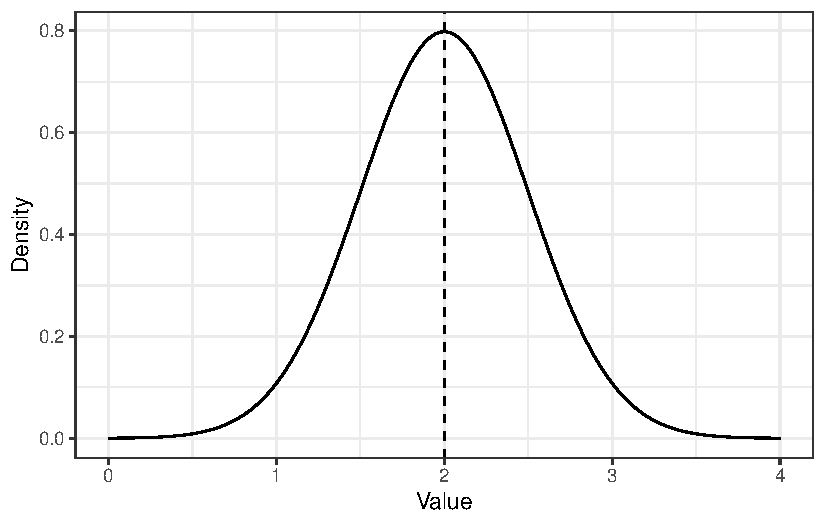
\includegraphics{andan-descriptives_files/figure-pdf/fig-norm-mode-1.pdf}

}

\caption{\label{fig-norm-mode}Нормальное распределение (μ~=~2\$,
σ~=~0.5). Пунктирной линией обозначено положение моды.}

\end{figure}%

\begin{figure}

\centering{

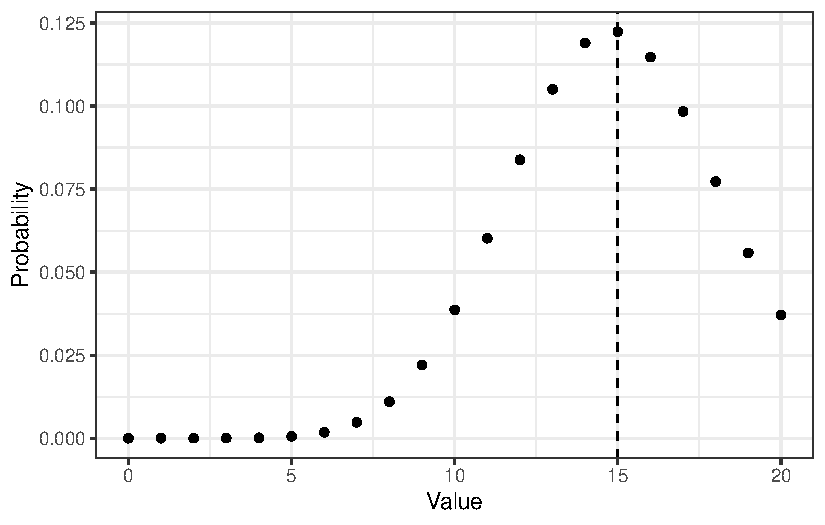
\includegraphics{andan-descriptives_files/figure-pdf/fig-binom-mode-1.pdf}

}

\caption{\label{fig-binom-mode}Биномиальное распределение (n~=~50,
p~=~0.3). Пунктирной линией обозначено положение моды.}

\end{figure}%

\begin{figure}

\centering{

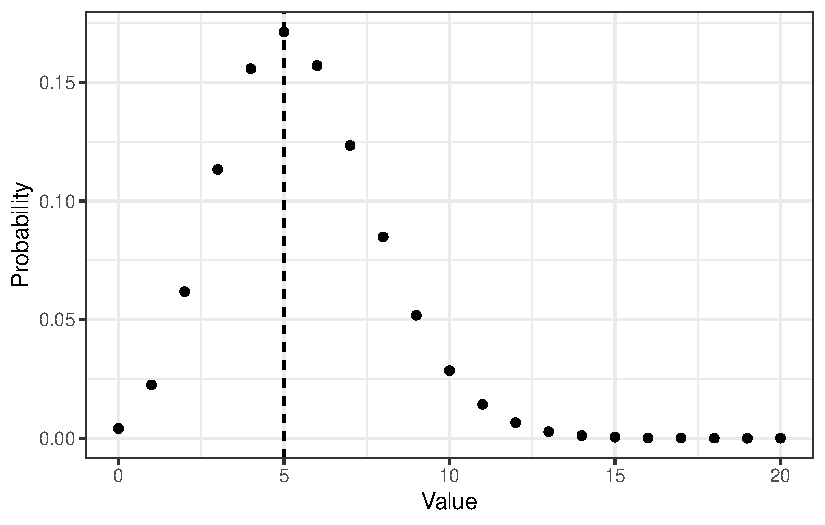
\includegraphics{andan-descriptives_files/figure-pdf/fig-poiss-mode-1.pdf}

}

\caption{\label{fig-poiss-mode}Распределение Пуассона (λ~=~5.5).
Пунктирной линией обозначено положение моды.}

\end{figure}%

Это теоретические распределения. С эмпирическими распределениями дело
обстоит так же, хотя они обычно менее гладенькие и красивые (см.
Рисунок~\ref{fig-mode-norm-sample} и
Рисунок~\ref{fig-mode-nbinom-sample}).

\begin{figure}

\centering{

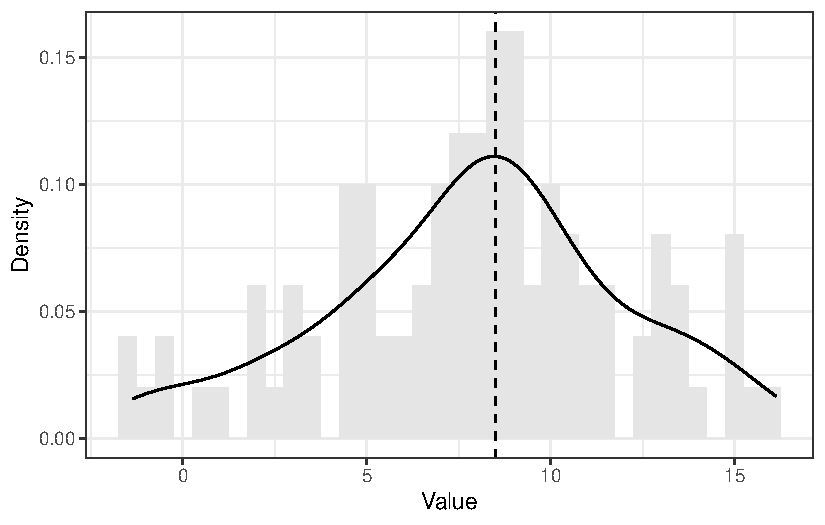
\includegraphics{andan-descriptives_files/figure-pdf/fig-mode-norm-sample-1.pdf}

}

\caption{\label{fig-mode-norm-sample}Эмпирическое распределение,
сгенерированное из нормального распределения (μ~=~8, σ~=~4, n~=~100).
\texttt{set.seed(314)}. Пунктирной линией обозначено положение моды.}

\end{figure}%

\begin{figure}

\centering{

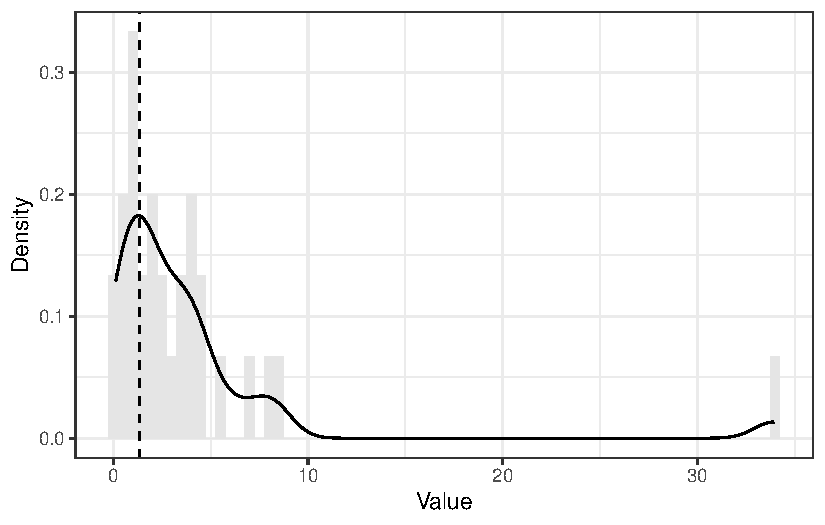
\includegraphics{andan-descriptives_files/figure-pdf/fig-mode-nbinom-sample-1.pdf}

}

\caption{\label{fig-mode-nbinom-sample}Эмпирическое распределение,
сгенерированное из логнормального распределения (μ~=~1.1, σ~=~1.39,
n~=~30). \texttt{set.seed(314)}. Пунктирной линией обозначено положение
моды.}

\end{figure}%

Однако на практике возможны и другие ситуации. Например, такие
(Рисунок~\ref{fig-bimodal}, Рисунок~\ref{fig-polymodal}):

\begin{figure}

\centering{

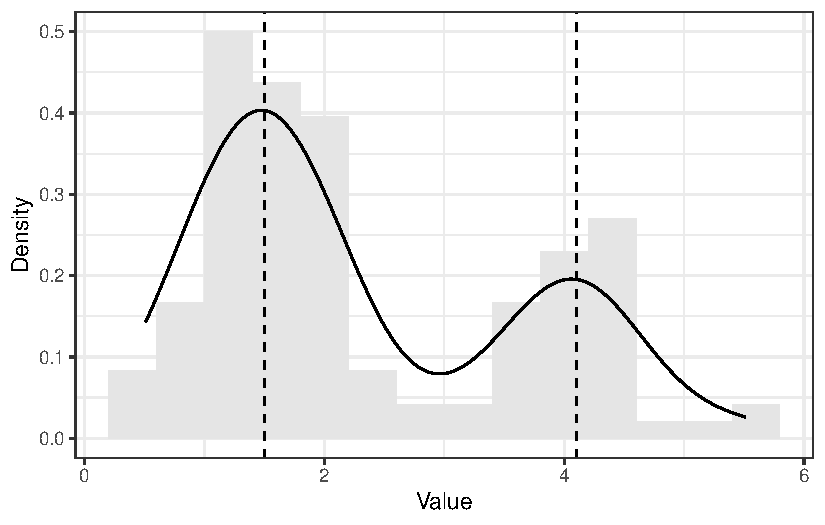
\includegraphics{andan-descriptives_files/figure-pdf/fig-bimodal-1.pdf}

}

\caption{\label{fig-bimodal}Бимодальное распределение. Сгенерировано из
двух нормальных распределений (μ1~=~1.5, σ1~=~0.4, n1~=~80; μ2~=~4,
σ2~=~0.5, n2~=~40). \texttt{set.seed(65)}. Пунктирными линиями
обозначены положения мод.}

\end{figure}%

\begin{figure}

\centering{

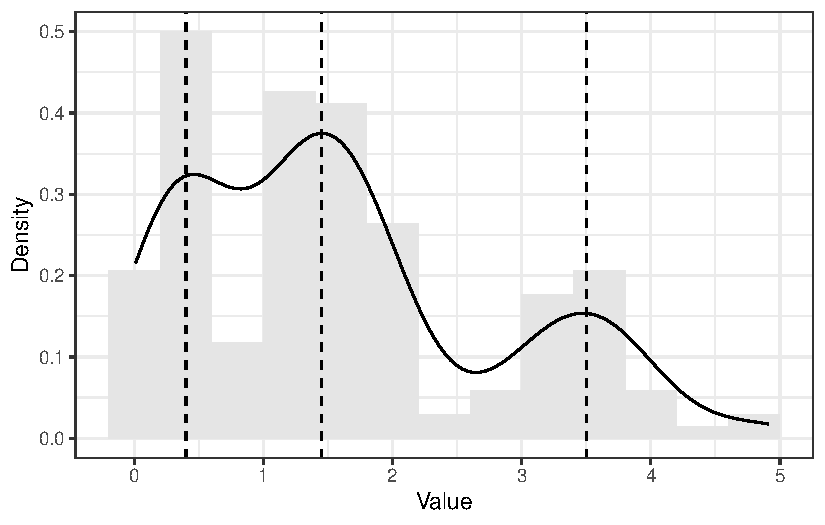
\includegraphics{andan-descriptives_files/figure-pdf/fig-polymodal-1.pdf}

}

\caption{\label{fig-polymodal}Полимодальное распределение. Сгенерировано
из двух нормальных распределений (μ1~=~1.5, σ1~=~0.3, n1~=~80; μ2~=~3.4,
σ2~=~0.5, n2~=~40) и бета-распределения (α~=~2, β~=~4, n~=~50).
\texttt{set.seed(65)}. Пунктирными линиями обозначены положения мод.}

\end{figure}%

В первом случае (Рисунок~\ref{fig-bimodal}) мы видим \emph{два локальных
максимума} функции плотности вероятности --- такое распределение
называется \textbf{бимодальным}. Во втором случае
(Рисунок~\ref{fig-polymodal}) функция плотности вероятности имеет
\emph{три локальных максимума} --- такое распределение называется
\textbf{полимодальным}. Бимональное распределение является частным
случаем полимодального распределения.

В прицнипе, пиков может быть и больше, однако при работе с реальными
данными чаще всего мы сталкиваемся с бимодальными распределениями.

\textbf{Что это значит и что с этим делать?}

Бимодальное распределение сигнализирует нам о \textbf{гетерогенности
выборки}. Если мы видим два выделяющихся пика, стоит подумать о том, что
наша выборка неоднородна и в ней выделяются две подвыборки. Посмотрим на
структуру выборки из примера выше (Рисунок~\ref{fig-bimodal-struct}):

\begin{figure}

\centering{

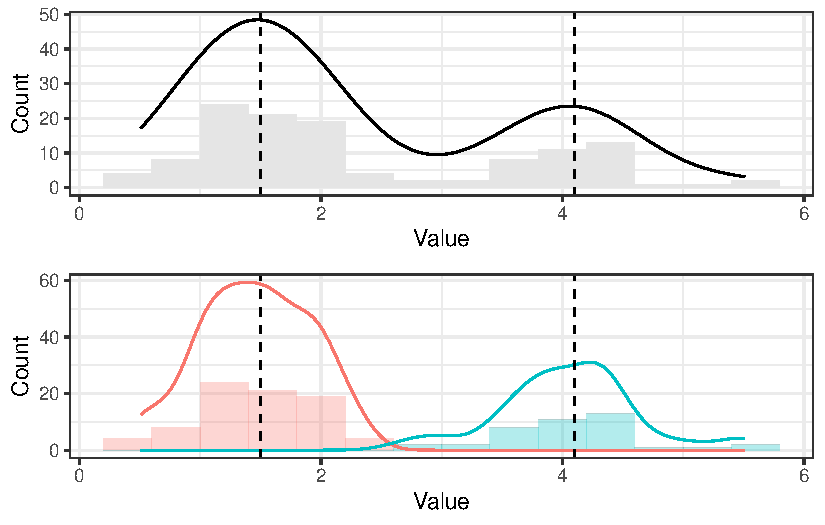
\includegraphics{andan-descriptives_files/figure-pdf/fig-bimodal-struct-1.pdf}

}

\caption{\label{fig-bimodal-struct}Структура бимодального распределения
из Рисунок~\ref{fig-bimodal}. Для удобства сопоставления графиков
плотностей вероятности по оси ординат отложены частоты.}

\end{figure}%

Действительно, наше распределение состоит из двух других распределений,
у каждого из которого есть своя мода --- поэтому итоговое распределение
получается бимодальным. Конечно, сейчас нам это очень удобно показать,
потому что мы знаем, как это распределение генерировалось. Когда же у
нас есть реальные данные и мы там наблюдаем такого «верблюда», бывает
достаточно сложно сказать, что «пошло не так».

Само по себе распределение не даст нам ответ на вопрос, почему оно
бимодальное --- чтобы выяснить причины такого поведения переменной нам
потребуются другие данные. Обычно у вас в данных есть «соцдем» --- пол,
возраст, сфера и место работы, уровень обрвазования и др. Попробуйте
построить распределение с разбиением исследуемой бимодальной переменной
по переменным «соцдема». Это, к сожалению, не является рецептом успеха,
поскольку причина гетерогенности выборки может и не содержаться в ваших
данных, но такое изучение данных станет хорошим показателем того, что вы
не просто «забили» на странное распределение своей переменной, а
поисследователи возможные его причины.

Если вам удалось найти причины гетерогенности выборки --- допустим, у
вас выделяются подвыборки «бакалавры» и «магистры» --- стоит подумать о
том, как обойтись с этой переменной в планируемом анализе, так как
игнорировать её, по-видимому, нельзя, поскольку она влияет на
вариатиность данных.

\begin{tcolorbox}[enhanced jigsaw, colback=white, bottomrule=.15mm, opacityback=0, opacitybacktitle=0.6, breakable, coltitle=black, colframe=quarto-callout-tip-color-frame, titlerule=0mm, rightrule=.15mm, bottomtitle=1mm, leftrule=.75mm, toptitle=1mm, left=2mm, arc=.35mm, title=\textcolor{quarto-callout-tip-color}{\faLightbulb}\hspace{0.5em}{Соцдем лишним не бывает}, colbacktitle=quarto-callout-tip-color!10!white, toprule=.15mm]

На этапе планирования исследования подумайте о том, чем могут отличаться
ваши респонденты или испытуемые между собой, помимо индивидуальных
различий.

\begin{itemize}
\tightlist
\item
  Если в эксперименте используете задачу мысленного вращения (mental
  rotation, \autocite{shepard71}), вполне возможно, испытуемые,
  работающие в сфере 3D-моделирования или дизайна интерьеров, могут
  сформировать подвыборку.
\item
  В случае HR-исследования, где фиксируется доход респондента,
  необходимо записать город, в котором он проживает и/или работает.
\item
  При изучении удовлетворенности городским пространством важными
  пунктами станут беременность, наличие/отсутствие детей,
  наличие/отсутствие автомобиля и др.
\end{itemize}

И так далее. Примеров для каждого случая можно подобрать много.

Стоит ли, скажем, в первом случае сразу исключить из выборки
3D-моделлеров? Зависит. От количества времени и денег на проведение
исследования. Однако \emph{как минимум эту информацию надо зафиксировать
в данных}. А решить, исключать ли этих респондентов из выборки или нет,
можно и позже. Главно об этом написать в отчете/статье, когда будете
описывать предобработку данных.

\end{tcolorbox}

\begin{center}\rule{0.5\linewidth}{0.5pt}\end{center}

\begin{tcolorbox}[enhanced jigsaw, colback=white, bottomrule=.15mm, opacityback=0, opacitybacktitle=0.6, breakable, coltitle=black, colframe=quarto-callout-warning-color-frame, titlerule=0mm, rightrule=.15mm, bottomtitle=1mm, leftrule=.75mm, toptitle=1mm, left=2mm, arc=.35mm, title=\textcolor{quarto-callout-warning-color}{\faExclamationTriangle}\hspace{0.5em}{Take-home: бимодальное распределение}, colbacktitle=quarto-callout-warning-color!10!white, toprule=.15mm]

\begin{itemize}
\tightlist
\item
  бимодальное распределение намекает на неоднородность данных --- скорее
  всего, в выборке есть две подвыборки
\item
  необходимо поискать в данных причины этой неодноросности, например, в
  социально-демографических переменных
\item
  если удалось найти переменную, объясняющую бимодальность, стоит
  подумать о том, как её учитывать в планируемом анализе
\end{itemize}

\end{tcolorbox}

\subsection{Медиана}\label{andan-descriptives-median}

Для номинальной шкалы мода --- это единственно возможная мера
центральной тенденции, потому что на этой шкале отсутствует порядок
элементов. На других шкалах наблюдения уже можно сортировать по
возрастнию или убыванию, поскольку начиная с ранговой (порядковой) шкалы
на всех них определена операция сравнения на «больше-меньше».

Возьмем тот же ряд наблюдений, что и в предыдущем разделе:

\[
\begin{bmatrix}
1 & 3 & 4 & 6 & 3 & 2 & 3 & 3 & 2 & 4 & 1
\end{bmatrix}
\]

Отсортируем наблюдения по возрастанию:

\[
\begin{bmatrix}
1  & 1 & 2 & 2 & 3 & 3 & 3 & 3 & 4 & 4 & 6
\end{bmatrix}
\]

Наша задача --- определить центральную тенденцию. Давайте посмотрим, что
оказалось в середине отсортированного ряда:

\[
\begin{bmatrix}
1 & 1 & 2 & 2 & 3 & \mathbf{3} & 3 & 3 & 4 & 4 & 6
\end{bmatrix}
\]

Это медиана. В данном случае она равна \(3\).

\begin{definition}[]\protect\hypertarget{def-median}{}\label{def-median}

\textbf{Медиана (median)} --- это значение, которое располагается на
середине отсортированного ряда значений переменной.

\end{definition}

Медиана делит все наблюдения переменной ровно пополам и половина
наблюдений оказывается по одну сторону от медианы, а половина --- по
другую.

Если число наблюдений нечётное, то всё ясно --- в середине
отсортированного ряда будет какое-то значение. А если число наблюдений
чётное? Тогда мы попадаем между значениями.

Возьмем для примера такой вектор наблюдений:

\[
\begin{bmatrix}
14 & 10 & 9 & 16 & 30 & 3 & 25 & 8 & 18 & 7
\end{bmatrix}
\]

Отсортируем:

\[
\begin{bmatrix}
3 & 7 & 8 & 9 & 10 & 14 & 16 & 18 & 25 & 30
\end{bmatrix}
\]

Найдем середину:

\[
\begin{bmatrix}
3 & 7 & 8 & 9 & 10 & | & 14 & 16 & 18 & 25 & 30
\end{bmatrix}
\]

В таком случае в качестве медианы берется среднее между двумя срединными
значениями:

\[
\text{median} = \frac{10 + 14}{2} = 12
\]

Итого, формализовать вычисление медианы можно следующим образом:

\begin{equation}\phantomsection\label{eq-median-formula}{
\text{median}(X) = X(a) =
\cases{
X\left(\frac{n+1}{2}\right), & if  2 | n \\
\dfrac{X(\frac{n}{2}) + X(\frac{n}{2} + 1)}{2}, & otherwise
}
}\end{equation}

где \(X\) --- ряд наблюдений случайной величины, \(n\) --- число
наблюдений, \(X(a)\) --- наблюдение с индексом \(a\) в отсортированном
векторе \(X\).

Если мы будем смотреть на медиану с позиции описания распределения, то
она будет той самой линией, которая разделит площадь под графиком
функции плотности вероятности пополам:

\begin{verbatim}
Warning in grid.Call.graphics(C_text, as.graphicsAnnot(x$label), x$x, x$y, :
conversion failure on 'эти значения' in 'mbcsToSbcs': dot substituted for <d1>
\end{verbatim}

\begin{verbatim}
Warning in grid.Call.graphics(C_text, as.graphicsAnnot(x$label), x$x, x$y, :
conversion failure on 'эти значения' in 'mbcsToSbcs': dot substituted for <8d>
\end{verbatim}

\begin{verbatim}
Warning in grid.Call.graphics(C_text, as.graphicsAnnot(x$label), x$x, x$y, :
conversion failure on 'эти значения' in 'mbcsToSbcs': dot substituted for <d1>
\end{verbatim}

\begin{verbatim}
Warning in grid.Call.graphics(C_text, as.graphicsAnnot(x$label), x$x, x$y, :
conversion failure on 'эти значения' in 'mbcsToSbcs': dot substituted for <82>
\end{verbatim}

\begin{verbatim}
Warning in grid.Call.graphics(C_text, as.graphicsAnnot(x$label), x$x, x$y, :
conversion failure on 'эти значения' in 'mbcsToSbcs': dot substituted for <d0>
\end{verbatim}

\begin{verbatim}
Warning in grid.Call.graphics(C_text, as.graphicsAnnot(x$label), x$x, x$y, :
conversion failure on 'эти значения' in 'mbcsToSbcs': dot substituted for <b8>
\end{verbatim}

\begin{verbatim}
Warning in grid.Call.graphics(C_text, as.graphicsAnnot(x$label), x$x, x$y, :
conversion failure on 'эти значения' in 'mbcsToSbcs': dot substituted for <d0>
\end{verbatim}

\begin{verbatim}
Warning in grid.Call.graphics(C_text, as.graphicsAnnot(x$label), x$x, x$y, :
conversion failure on 'эти значения' in 'mbcsToSbcs': dot substituted for <b7>
\end{verbatim}

\begin{verbatim}
Warning in grid.Call.graphics(C_text, as.graphicsAnnot(x$label), x$x, x$y, :
conversion failure on 'эти значения' in 'mbcsToSbcs': dot substituted for <d0>
\end{verbatim}

\begin{verbatim}
Warning in grid.Call.graphics(C_text, as.graphicsAnnot(x$label), x$x, x$y, :
conversion failure on 'эти значения' in 'mbcsToSbcs': dot substituted for <bd>
\end{verbatim}

\begin{verbatim}
Warning in grid.Call.graphics(C_text, as.graphicsAnnot(x$label), x$x, x$y, :
conversion failure on 'эти значения' in 'mbcsToSbcs': dot substituted for <d0>
\end{verbatim}

\begin{verbatim}
Warning in grid.Call.graphics(C_text, as.graphicsAnnot(x$label), x$x, x$y, :
conversion failure on 'эти значения' in 'mbcsToSbcs': dot substituted for <b0>
\end{verbatim}

\begin{verbatim}
Warning in grid.Call.graphics(C_text, as.graphicsAnnot(x$label), x$x, x$y, :
conversion failure on 'эти значения' in 'mbcsToSbcs': dot substituted for <d1>
\end{verbatim}

\begin{verbatim}
Warning in grid.Call.graphics(C_text, as.graphicsAnnot(x$label), x$x, x$y, :
conversion failure on 'эти значения' in 'mbcsToSbcs': dot substituted for <87>
\end{verbatim}

\begin{verbatim}
Warning in grid.Call.graphics(C_text, as.graphicsAnnot(x$label), x$x, x$y, :
conversion failure on 'эти значения' in 'mbcsToSbcs': dot substituted for <d0>
\end{verbatim}

\begin{verbatim}
Warning in grid.Call.graphics(C_text, as.graphicsAnnot(x$label), x$x, x$y, :
conversion failure on 'эти значения' in 'mbcsToSbcs': dot substituted for <b5>
\end{verbatim}

\begin{verbatim}
Warning in grid.Call.graphics(C_text, as.graphicsAnnot(x$label), x$x, x$y, :
conversion failure on 'эти значения' in 'mbcsToSbcs': dot substituted for <d0>
\end{verbatim}

\begin{verbatim}
Warning in grid.Call.graphics(C_text, as.graphicsAnnot(x$label), x$x, x$y, :
conversion failure on 'эти значения' in 'mbcsToSbcs': dot substituted for <bd>
\end{verbatim}

\begin{verbatim}
Warning in grid.Call.graphics(C_text, as.graphicsAnnot(x$label), x$x, x$y, :
conversion failure on 'эти значения' in 'mbcsToSbcs': dot substituted for <d0>
\end{verbatim}

\begin{verbatim}
Warning in grid.Call.graphics(C_text, as.graphicsAnnot(x$label), x$x, x$y, :
conversion failure on 'эти значения' in 'mbcsToSbcs': dot substituted for <b8>
\end{verbatim}

\begin{verbatim}
Warning in grid.Call.graphics(C_text, as.graphicsAnnot(x$label), x$x, x$y, :
conversion failure on 'эти значения' in 'mbcsToSbcs': dot substituted for <d1>
\end{verbatim}

\begin{verbatim}
Warning in grid.Call.graphics(C_text, as.graphicsAnnot(x$label), x$x, x$y, :
conversion failure on 'эти значения' in 'mbcsToSbcs': dot substituted for <8f>
\end{verbatim}

\begin{verbatim}
Warning in grid.Call.graphics(C_text, as.graphicsAnnot(x$label), x$x, x$y, :
conversion failure on 'больше медианы ' in 'mbcsToSbcs': dot substituted for
<d0>
\end{verbatim}

\begin{verbatim}
Warning in grid.Call.graphics(C_text, as.graphicsAnnot(x$label), x$x, x$y, :
conversion failure on 'больше медианы ' in 'mbcsToSbcs': dot substituted for
<b1>
\end{verbatim}

\begin{verbatim}
Warning in grid.Call.graphics(C_text, as.graphicsAnnot(x$label), x$x, x$y, :
conversion failure on 'больше медианы ' in 'mbcsToSbcs': dot substituted for
<d0>
\end{verbatim}

\begin{verbatim}
Warning in grid.Call.graphics(C_text, as.graphicsAnnot(x$label), x$x, x$y, :
conversion failure on 'больше медианы ' in 'mbcsToSbcs': dot substituted for
<be>
\end{verbatim}

\begin{verbatim}
Warning in grid.Call.graphics(C_text, as.graphicsAnnot(x$label), x$x, x$y, :
conversion failure on 'больше медианы ' in 'mbcsToSbcs': dot substituted for
<d0>
\end{verbatim}

\begin{verbatim}
Warning in grid.Call.graphics(C_text, as.graphicsAnnot(x$label), x$x, x$y, :
conversion failure on 'больше медианы ' in 'mbcsToSbcs': dot substituted for
<bb>
\end{verbatim}

\begin{verbatim}
Warning in grid.Call.graphics(C_text, as.graphicsAnnot(x$label), x$x, x$y, :
conversion failure on 'больше медианы ' in 'mbcsToSbcs': dot substituted for
<d1>
\end{verbatim}

\begin{verbatim}
Warning in grid.Call.graphics(C_text, as.graphicsAnnot(x$label), x$x, x$y, :
conversion failure on 'больше медианы ' in 'mbcsToSbcs': dot substituted for
<8c>
\end{verbatim}

\begin{verbatim}
Warning in grid.Call.graphics(C_text, as.graphicsAnnot(x$label), x$x, x$y, :
conversion failure on 'больше медианы ' in 'mbcsToSbcs': dot substituted for
<d1>
\end{verbatim}

\begin{verbatim}
Warning in grid.Call.graphics(C_text, as.graphicsAnnot(x$label), x$x, x$y, :
conversion failure on 'больше медианы ' in 'mbcsToSbcs': dot substituted for
<88>
\end{verbatim}

\begin{verbatim}
Warning in grid.Call.graphics(C_text, as.graphicsAnnot(x$label), x$x, x$y, :
conversion failure on 'больше медианы ' in 'mbcsToSbcs': dot substituted for
<d0>
\end{verbatim}

\begin{verbatim}
Warning in grid.Call.graphics(C_text, as.graphicsAnnot(x$label), x$x, x$y, :
conversion failure on 'больше медианы ' in 'mbcsToSbcs': dot substituted for
<b5>
\end{verbatim}

\begin{verbatim}
Warning in grid.Call.graphics(C_text, as.graphicsAnnot(x$label), x$x, x$y, :
conversion failure on 'больше медианы ' in 'mbcsToSbcs': dot substituted for
<d0>
\end{verbatim}

\begin{verbatim}
Warning in grid.Call.graphics(C_text, as.graphicsAnnot(x$label), x$x, x$y, :
conversion failure on 'больше медианы ' in 'mbcsToSbcs': dot substituted for
<bc>
\end{verbatim}

\begin{verbatim}
Warning in grid.Call.graphics(C_text, as.graphicsAnnot(x$label), x$x, x$y, :
conversion failure on 'больше медианы ' in 'mbcsToSbcs': dot substituted for
<d0>
\end{verbatim}

\begin{verbatim}
Warning in grid.Call.graphics(C_text, as.graphicsAnnot(x$label), x$x, x$y, :
conversion failure on 'больше медианы ' in 'mbcsToSbcs': dot substituted for
<b5>
\end{verbatim}

\begin{verbatim}
Warning in grid.Call.graphics(C_text, as.graphicsAnnot(x$label), x$x, x$y, :
conversion failure on 'больше медианы ' in 'mbcsToSbcs': dot substituted for
<d0>
\end{verbatim}

\begin{verbatim}
Warning in grid.Call.graphics(C_text, as.graphicsAnnot(x$label), x$x, x$y, :
conversion failure on 'больше медианы ' in 'mbcsToSbcs': dot substituted for
<b4>
\end{verbatim}

\begin{verbatim}
Warning in grid.Call.graphics(C_text, as.graphicsAnnot(x$label), x$x, x$y, :
conversion failure on 'больше медианы ' in 'mbcsToSbcs': dot substituted for
<d0>
\end{verbatim}

\begin{verbatim}
Warning in grid.Call.graphics(C_text, as.graphicsAnnot(x$label), x$x, x$y, :
conversion failure on 'больше медианы ' in 'mbcsToSbcs': dot substituted for
<b8>
\end{verbatim}

\begin{verbatim}
Warning in grid.Call.graphics(C_text, as.graphicsAnnot(x$label), x$x, x$y, :
conversion failure on 'больше медианы ' in 'mbcsToSbcs': dot substituted for
<d0>
\end{verbatim}

\begin{verbatim}
Warning in grid.Call.graphics(C_text, as.graphicsAnnot(x$label), x$x, x$y, :
conversion failure on 'больше медианы ' in 'mbcsToSbcs': dot substituted for
<b0>
\end{verbatim}

\begin{verbatim}
Warning in grid.Call.graphics(C_text, as.graphicsAnnot(x$label), x$x, x$y, :
conversion failure on 'больше медианы ' in 'mbcsToSbcs': dot substituted for
<d0>
\end{verbatim}

\begin{verbatim}
Warning in grid.Call.graphics(C_text, as.graphicsAnnot(x$label), x$x, x$y, :
conversion failure on 'больше медианы ' in 'mbcsToSbcs': dot substituted for
<bd>
\end{verbatim}

\begin{verbatim}
Warning in grid.Call.graphics(C_text, as.graphicsAnnot(x$label), x$x, x$y, :
conversion failure on 'больше медианы ' in 'mbcsToSbcs': dot substituted for
<d1>
\end{verbatim}

\begin{verbatim}
Warning in grid.Call.graphics(C_text, as.graphicsAnnot(x$label), x$x, x$y, :
conversion failure on 'больше медианы ' in 'mbcsToSbcs': dot substituted for
<8b>
\end{verbatim}

\begin{verbatim}
Warning in grid.Call.graphics(C_text, as.graphicsAnnot(x$label), x$x, x$y, :
conversion failure on 'эти значения' in 'mbcsToSbcs': dot substituted for <d1>
\end{verbatim}

\begin{verbatim}
Warning in grid.Call.graphics(C_text, as.graphicsAnnot(x$label), x$x, x$y, :
conversion failure on 'эти значения' in 'mbcsToSbcs': dot substituted for <8d>
\end{verbatim}

\begin{verbatim}
Warning in grid.Call.graphics(C_text, as.graphicsAnnot(x$label), x$x, x$y, :
conversion failure on 'эти значения' in 'mbcsToSbcs': dot substituted for <d1>
\end{verbatim}

\begin{verbatim}
Warning in grid.Call.graphics(C_text, as.graphicsAnnot(x$label), x$x, x$y, :
conversion failure on 'эти значения' in 'mbcsToSbcs': dot substituted for <82>
\end{verbatim}

\begin{verbatim}
Warning in grid.Call.graphics(C_text, as.graphicsAnnot(x$label), x$x, x$y, :
conversion failure on 'эти значения' in 'mbcsToSbcs': dot substituted for <d0>
\end{verbatim}

\begin{verbatim}
Warning in grid.Call.graphics(C_text, as.graphicsAnnot(x$label), x$x, x$y, :
conversion failure on 'эти значения' in 'mbcsToSbcs': dot substituted for <b8>
\end{verbatim}

\begin{verbatim}
Warning in grid.Call.graphics(C_text, as.graphicsAnnot(x$label), x$x, x$y, :
conversion failure on 'эти значения' in 'mbcsToSbcs': dot substituted for <d0>
\end{verbatim}

\begin{verbatim}
Warning in grid.Call.graphics(C_text, as.graphicsAnnot(x$label), x$x, x$y, :
conversion failure on 'эти значения' in 'mbcsToSbcs': dot substituted for <b7>
\end{verbatim}

\begin{verbatim}
Warning in grid.Call.graphics(C_text, as.graphicsAnnot(x$label), x$x, x$y, :
conversion failure on 'эти значения' in 'mbcsToSbcs': dot substituted for <d0>
\end{verbatim}

\begin{verbatim}
Warning in grid.Call.graphics(C_text, as.graphicsAnnot(x$label), x$x, x$y, :
conversion failure on 'эти значения' in 'mbcsToSbcs': dot substituted for <bd>
\end{verbatim}

\begin{verbatim}
Warning in grid.Call.graphics(C_text, as.graphicsAnnot(x$label), x$x, x$y, :
conversion failure on 'эти значения' in 'mbcsToSbcs': dot substituted for <d0>
\end{verbatim}

\begin{verbatim}
Warning in grid.Call.graphics(C_text, as.graphicsAnnot(x$label), x$x, x$y, :
conversion failure on 'эти значения' in 'mbcsToSbcs': dot substituted for <b0>
\end{verbatim}

\begin{verbatim}
Warning in grid.Call.graphics(C_text, as.graphicsAnnot(x$label), x$x, x$y, :
conversion failure on 'эти значения' in 'mbcsToSbcs': dot substituted for <d1>
\end{verbatim}

\begin{verbatim}
Warning in grid.Call.graphics(C_text, as.graphicsAnnot(x$label), x$x, x$y, :
conversion failure on 'эти значения' in 'mbcsToSbcs': dot substituted for <87>
\end{verbatim}

\begin{verbatim}
Warning in grid.Call.graphics(C_text, as.graphicsAnnot(x$label), x$x, x$y, :
conversion failure on 'эти значения' in 'mbcsToSbcs': dot substituted for <d0>
\end{verbatim}

\begin{verbatim}
Warning in grid.Call.graphics(C_text, as.graphicsAnnot(x$label), x$x, x$y, :
conversion failure on 'эти значения' in 'mbcsToSbcs': dot substituted for <b5>
\end{verbatim}

\begin{verbatim}
Warning in grid.Call.graphics(C_text, as.graphicsAnnot(x$label), x$x, x$y, :
conversion failure on 'эти значения' in 'mbcsToSbcs': dot substituted for <d0>
\end{verbatim}

\begin{verbatim}
Warning in grid.Call.graphics(C_text, as.graphicsAnnot(x$label), x$x, x$y, :
conversion failure on 'эти значения' in 'mbcsToSbcs': dot substituted for <bd>
\end{verbatim}

\begin{verbatim}
Warning in grid.Call.graphics(C_text, as.graphicsAnnot(x$label), x$x, x$y, :
conversion failure on 'эти значения' in 'mbcsToSbcs': dot substituted for <d0>
\end{verbatim}

\begin{verbatim}
Warning in grid.Call.graphics(C_text, as.graphicsAnnot(x$label), x$x, x$y, :
conversion failure on 'эти значения' in 'mbcsToSbcs': dot substituted for <b8>
\end{verbatim}

\begin{verbatim}
Warning in grid.Call.graphics(C_text, as.graphicsAnnot(x$label), x$x, x$y, :
conversion failure on 'эти значения' in 'mbcsToSbcs': dot substituted for <d1>
\end{verbatim}

\begin{verbatim}
Warning in grid.Call.graphics(C_text, as.graphicsAnnot(x$label), x$x, x$y, :
conversion failure on 'эти значения' in 'mbcsToSbcs': dot substituted for <8f>
\end{verbatim}

\begin{verbatim}
Warning in grid.Call.graphics(C_text, as.graphicsAnnot(x$label), x$x, x$y, :
conversion failure on 'меньше медианы ' in 'mbcsToSbcs': dot substituted for
<d0>
\end{verbatim}

\begin{verbatim}
Warning in grid.Call.graphics(C_text, as.graphicsAnnot(x$label), x$x, x$y, :
conversion failure on 'меньше медианы ' in 'mbcsToSbcs': dot substituted for
<bc>
\end{verbatim}

\begin{verbatim}
Warning in grid.Call.graphics(C_text, as.graphicsAnnot(x$label), x$x, x$y, :
conversion failure on 'меньше медианы ' in 'mbcsToSbcs': dot substituted for
<d0>
\end{verbatim}

\begin{verbatim}
Warning in grid.Call.graphics(C_text, as.graphicsAnnot(x$label), x$x, x$y, :
conversion failure on 'меньше медианы ' in 'mbcsToSbcs': dot substituted for
<b5>
\end{verbatim}

\begin{verbatim}
Warning in grid.Call.graphics(C_text, as.graphicsAnnot(x$label), x$x, x$y, :
conversion failure on 'меньше медианы ' in 'mbcsToSbcs': dot substituted for
<d0>
\end{verbatim}

\begin{verbatim}
Warning in grid.Call.graphics(C_text, as.graphicsAnnot(x$label), x$x, x$y, :
conversion failure on 'меньше медианы ' in 'mbcsToSbcs': dot substituted for
<bd>
\end{verbatim}

\begin{verbatim}
Warning in grid.Call.graphics(C_text, as.graphicsAnnot(x$label), x$x, x$y, :
conversion failure on 'меньше медианы ' in 'mbcsToSbcs': dot substituted for
<d1>
\end{verbatim}

\begin{verbatim}
Warning in grid.Call.graphics(C_text, as.graphicsAnnot(x$label), x$x, x$y, :
conversion failure on 'меньше медианы ' in 'mbcsToSbcs': dot substituted for
<8c>
\end{verbatim}

\begin{verbatim}
Warning in grid.Call.graphics(C_text, as.graphicsAnnot(x$label), x$x, x$y, :
conversion failure on 'меньше медианы ' in 'mbcsToSbcs': dot substituted for
<d1>
\end{verbatim}

\begin{verbatim}
Warning in grid.Call.graphics(C_text, as.graphicsAnnot(x$label), x$x, x$y, :
conversion failure on 'меньше медианы ' in 'mbcsToSbcs': dot substituted for
<88>
\end{verbatim}

\begin{verbatim}
Warning in grid.Call.graphics(C_text, as.graphicsAnnot(x$label), x$x, x$y, :
conversion failure on 'меньше медианы ' in 'mbcsToSbcs': dot substituted for
<d0>
\end{verbatim}

\begin{verbatim}
Warning in grid.Call.graphics(C_text, as.graphicsAnnot(x$label), x$x, x$y, :
conversion failure on 'меньше медианы ' in 'mbcsToSbcs': dot substituted for
<b5>
\end{verbatim}

\begin{verbatim}
Warning in grid.Call.graphics(C_text, as.graphicsAnnot(x$label), x$x, x$y, :
conversion failure on 'меньше медианы ' in 'mbcsToSbcs': dot substituted for
<d0>
\end{verbatim}

\begin{verbatim}
Warning in grid.Call.graphics(C_text, as.graphicsAnnot(x$label), x$x, x$y, :
conversion failure on 'меньше медианы ' in 'mbcsToSbcs': dot substituted for
<bc>
\end{verbatim}

\begin{verbatim}
Warning in grid.Call.graphics(C_text, as.graphicsAnnot(x$label), x$x, x$y, :
conversion failure on 'меньше медианы ' in 'mbcsToSbcs': dot substituted for
<d0>
\end{verbatim}

\begin{verbatim}
Warning in grid.Call.graphics(C_text, as.graphicsAnnot(x$label), x$x, x$y, :
conversion failure on 'меньше медианы ' in 'mbcsToSbcs': dot substituted for
<b5>
\end{verbatim}

\begin{verbatim}
Warning in grid.Call.graphics(C_text, as.graphicsAnnot(x$label), x$x, x$y, :
conversion failure on 'меньше медианы ' in 'mbcsToSbcs': dot substituted for
<d0>
\end{verbatim}

\begin{verbatim}
Warning in grid.Call.graphics(C_text, as.graphicsAnnot(x$label), x$x, x$y, :
conversion failure on 'меньше медианы ' in 'mbcsToSbcs': dot substituted for
<b4>
\end{verbatim}

\begin{verbatim}
Warning in grid.Call.graphics(C_text, as.graphicsAnnot(x$label), x$x, x$y, :
conversion failure on 'меньше медианы ' in 'mbcsToSbcs': dot substituted for
<d0>
\end{verbatim}

\begin{verbatim}
Warning in grid.Call.graphics(C_text, as.graphicsAnnot(x$label), x$x, x$y, :
conversion failure on 'меньше медианы ' in 'mbcsToSbcs': dot substituted for
<b8>
\end{verbatim}

\begin{verbatim}
Warning in grid.Call.graphics(C_text, as.graphicsAnnot(x$label), x$x, x$y, :
conversion failure on 'меньше медианы ' in 'mbcsToSbcs': dot substituted for
<d0>
\end{verbatim}

\begin{verbatim}
Warning in grid.Call.graphics(C_text, as.graphicsAnnot(x$label), x$x, x$y, :
conversion failure on 'меньше медианы ' in 'mbcsToSbcs': dot substituted for
<b0>
\end{verbatim}

\begin{verbatim}
Warning in grid.Call.graphics(C_text, as.graphicsAnnot(x$label), x$x, x$y, :
conversion failure on 'меньше медианы ' in 'mbcsToSbcs': dot substituted for
<d0>
\end{verbatim}

\begin{verbatim}
Warning in grid.Call.graphics(C_text, as.graphicsAnnot(x$label), x$x, x$y, :
conversion failure on 'меньше медианы ' in 'mbcsToSbcs': dot substituted for
<bd>
\end{verbatim}

\begin{verbatim}
Warning in grid.Call.graphics(C_text, as.graphicsAnnot(x$label), x$x, x$y, :
conversion failure on 'меньше медианы ' in 'mbcsToSbcs': dot substituted for
<d1>
\end{verbatim}

\begin{verbatim}
Warning in grid.Call.graphics(C_text, as.graphicsAnnot(x$label), x$x, x$y, :
conversion failure on 'меньше медианы ' in 'mbcsToSbcs': dot substituted for
<8b>
\end{verbatim}

\begin{verbatim}
Warning in grid.Call.graphics(C_text, as.graphicsAnnot(x$label), x$x, x$y, :
conversion failure on 'это медиана' in 'mbcsToSbcs': dot substituted for <d1>
\end{verbatim}

\begin{verbatim}
Warning in grid.Call.graphics(C_text, as.graphicsAnnot(x$label), x$x, x$y, :
conversion failure on 'это медиана' in 'mbcsToSbcs': dot substituted for <8d>
\end{verbatim}

\begin{verbatim}
Warning in grid.Call.graphics(C_text, as.graphicsAnnot(x$label), x$x, x$y, :
conversion failure on 'это медиана' in 'mbcsToSbcs': dot substituted for <d1>
\end{verbatim}

\begin{verbatim}
Warning in grid.Call.graphics(C_text, as.graphicsAnnot(x$label), x$x, x$y, :
conversion failure on 'это медиана' in 'mbcsToSbcs': dot substituted for <82>
\end{verbatim}

\begin{verbatim}
Warning in grid.Call.graphics(C_text, as.graphicsAnnot(x$label), x$x, x$y, :
conversion failure on 'это медиана' in 'mbcsToSbcs': dot substituted for <d0>
\end{verbatim}

\begin{verbatim}
Warning in grid.Call.graphics(C_text, as.graphicsAnnot(x$label), x$x, x$y, :
conversion failure on 'это медиана' in 'mbcsToSbcs': dot substituted for <be>
\end{verbatim}

\begin{verbatim}
Warning in grid.Call.graphics(C_text, as.graphicsAnnot(x$label), x$x, x$y, :
conversion failure on 'это медиана' in 'mbcsToSbcs': dot substituted for <d0>
\end{verbatim}

\begin{verbatim}
Warning in grid.Call.graphics(C_text, as.graphicsAnnot(x$label), x$x, x$y, :
conversion failure on 'это медиана' in 'mbcsToSbcs': dot substituted for <bc>
\end{verbatim}

\begin{verbatim}
Warning in grid.Call.graphics(C_text, as.graphicsAnnot(x$label), x$x, x$y, :
conversion failure on 'это медиана' in 'mbcsToSbcs': dot substituted for <d0>
\end{verbatim}

\begin{verbatim}
Warning in grid.Call.graphics(C_text, as.graphicsAnnot(x$label), x$x, x$y, :
conversion failure on 'это медиана' in 'mbcsToSbcs': dot substituted for <b5>
\end{verbatim}

\begin{verbatim}
Warning in grid.Call.graphics(C_text, as.graphicsAnnot(x$label), x$x, x$y, :
conversion failure on 'это медиана' in 'mbcsToSbcs': dot substituted for <d0>
\end{verbatim}

\begin{verbatim}
Warning in grid.Call.graphics(C_text, as.graphicsAnnot(x$label), x$x, x$y, :
conversion failure on 'это медиана' in 'mbcsToSbcs': dot substituted for <b4>
\end{verbatim}

\begin{verbatim}
Warning in grid.Call.graphics(C_text, as.graphicsAnnot(x$label), x$x, x$y, :
conversion failure on 'это медиана' in 'mbcsToSbcs': dot substituted for <d0>
\end{verbatim}

\begin{verbatim}
Warning in grid.Call.graphics(C_text, as.graphicsAnnot(x$label), x$x, x$y, :
conversion failure on 'это медиана' in 'mbcsToSbcs': dot substituted for <b8>
\end{verbatim}

\begin{verbatim}
Warning in grid.Call.graphics(C_text, as.graphicsAnnot(x$label), x$x, x$y, :
conversion failure on 'это медиана' in 'mbcsToSbcs': dot substituted for <d0>
\end{verbatim}

\begin{verbatim}
Warning in grid.Call.graphics(C_text, as.graphicsAnnot(x$label), x$x, x$y, :
conversion failure on 'это медиана' in 'mbcsToSbcs': dot substituted for <b0>
\end{verbatim}

\begin{verbatim}
Warning in grid.Call.graphics(C_text, as.graphicsAnnot(x$label), x$x, x$y, :
conversion failure on 'это медиана' in 'mbcsToSbcs': dot substituted for <d0>
\end{verbatim}

\begin{verbatim}
Warning in grid.Call.graphics(C_text, as.graphicsAnnot(x$label), x$x, x$y, :
conversion failure on 'это медиана' in 'mbcsToSbcs': dot substituted for <bd>
\end{verbatim}

\begin{verbatim}
Warning in grid.Call.graphics(C_text, as.graphicsAnnot(x$label), x$x, x$y, :
conversion failure on 'это медиана' in 'mbcsToSbcs': dot substituted for <d0>
\end{verbatim}

\begin{verbatim}
Warning in grid.Call.graphics(C_text, as.graphicsAnnot(x$label), x$x, x$y, :
conversion failure on 'это медиана' in 'mbcsToSbcs': dot substituted for <b0>
\end{verbatim}

\begin{figure}

\centering{

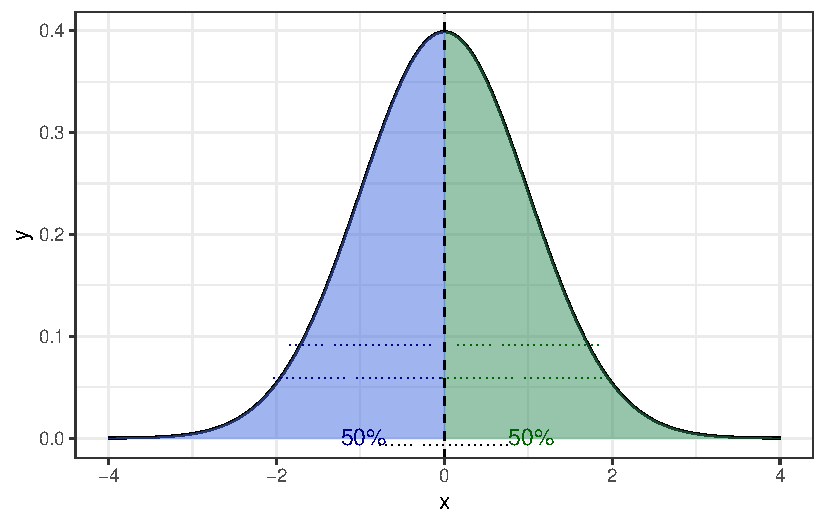
\includegraphics{andan-descriptives_files/figure-pdf/fig-median-norm-1.pdf}

}

\caption{\label{fig-median-norm}Медиана нормального распределения}

\end{figure}%

При этом форма распределения не имеет значения --- площадь под графиком
всегда будет делиться пополам:

\begin{figure}

\centering{

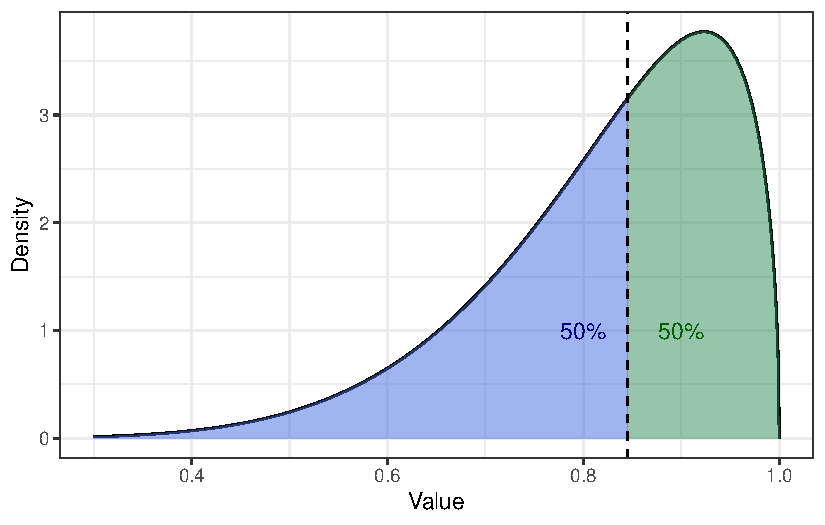
\includegraphics{andan-descriptives_files/figure-pdf/fig-median-left-skew-1.pdf}

}

\caption{\label{fig-median-left-skew}Медиана распределения с
отрицательной асимметрией.}

\end{figure}%

\begin{figure}

\centering{

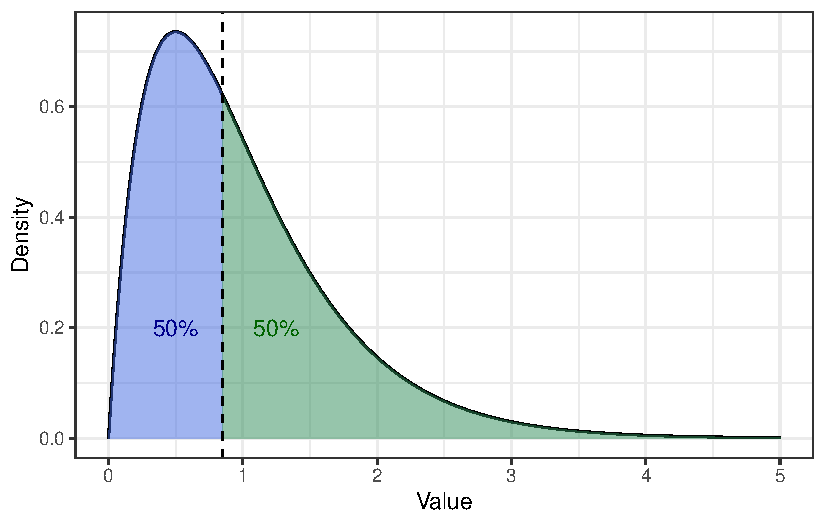
\includegraphics{andan-descriptives_files/figure-pdf/fig-median-right-skew-1.pdf}

}

\caption{\label{fig-median-right-skew}Медиана распределения с
положительной асимметрией.}

\end{figure}%

\begin{figure}

\centering{

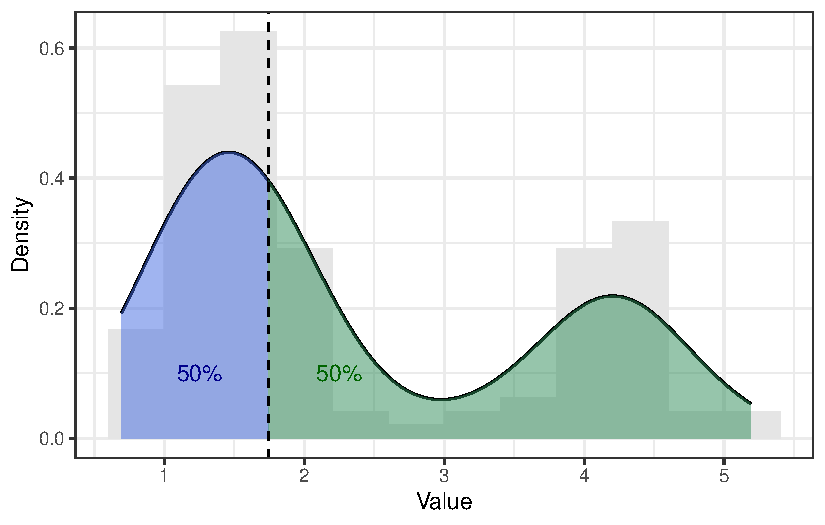
\includegraphics{andan-descriptives_files/figure-pdf/fig-median-bimodal-1.pdf}

}

\caption{\label{fig-median-bimodal}Медиана бимодального распределения.}

\end{figure}%

\begin{center}\rule{0.5\linewidth}{0.5pt}\end{center}

\begin{tcolorbox}[enhanced jigsaw, colback=white, bottomrule=.15mm, opacityback=0, opacitybacktitle=0.6, breakable, coltitle=black, colframe=quarto-callout-warning-color-frame, titlerule=0mm, rightrule=.15mm, bottomtitle=1mm, leftrule=.75mm, toptitle=1mm, left=2mm, arc=.35mm, title=\textcolor{quarto-callout-warning-color}{\faExclamationTriangle}\hspace{0.5em}{Take-home: медиана}, colbacktitle=quarto-callout-warning-color!10!white, toprule=.15mm]

\begin{itemize}
\tightlist
\item
  медиану можно расчитать только на шкалах, где задан порядок (ранговая,
  интервальная, абсолютная)
\item
  медиана делит выборку наблюдений на две равные части
\item
  линия медианы раздели площадь под графиком функции плотности
  вероятности пополам
\end{itemize}

\end{tcolorbox}

\subsection{Среднее}\label{andan-descriptives-mean}

Если наша переменная измерена в самых мощных шкалах --- интервальной или
абсолютной --- то нам доступна ещё одна мера центральной тенденции.

\subsubsection{Арифметическое
среднее}\label{andan-descriptives-arithmetic-mean}

С этим существом все знакомы еще со школы. \textbf{Арифметическое
среднее (arithmetic mean, mean, average)} считается так:

\[
M_{X} = \bar x = \dfrac{\sum_{i=1}^{n}x_i}{n},
\]

где \(\bar X\) --- среднее арифметическое, \(x_i\) --- наблюдение в
векторе \(X\), \(n\) --- количество наблюдений.

Ну, то есть всё сложить и поделить на количество того, чего сложили.
Изи.

\paragraph{Свойства среднего
арифметического}\label{andan-descriptives-arithmetic-mean-features}

\begin{itemize}
\tightlist
\item
  \textbf{Если к каждому значению распределения прибавить некоторое
  число (константу), то среднее увеличится на это же константу.}
\end{itemize}

\[
M_{X+c} = M_X + c
\]

Вот почему:

\[
M_{X+c} = \frac{\sum_{i=1}^n (x_i + c)}{n} = \frac{\sum_{i=1}^n x_i + nc}{n} = \frac{\sum_{i=1}^n x_i}{n} + c = M_X + c
\]

Иначе говоря, распределение просто сдвинется. Например, если к каждому
значению синего распределения прибавить \(2\), получится красное:

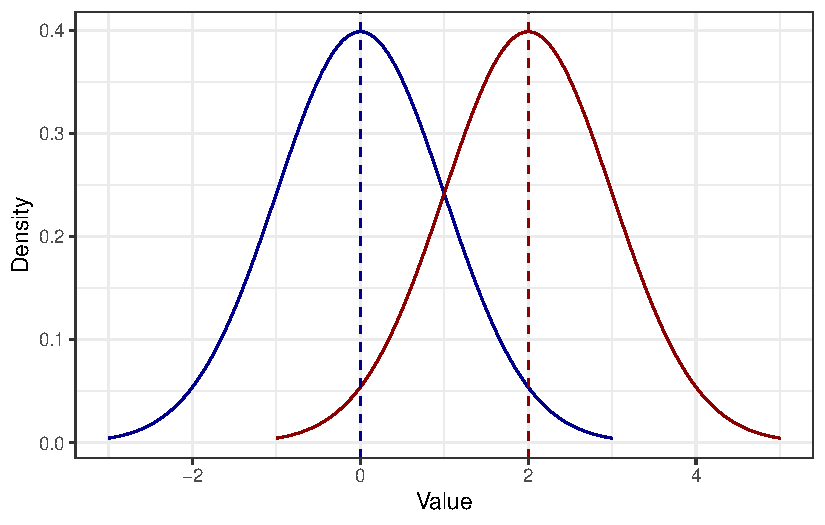
\includegraphics{andan-descriptives_files/figure-pdf/mean_feature_1-1.pdf}

\begin{itemize}
\tightlist
\item
  \textbf{Если каждое значение распределение умножить на некоторое число
  (константу), то среднее увеличится во столько же раз.}
\end{itemize}

\[
M_{X \times c} = M_X \times c
\]

Вот почему:

\[
M_{X \times c} = \frac{\sum_{i=1}^n (x_i \times c)}{n} = \frac{c \times \sum_{i=1}^n x_i}{n} = \frac{\sum_{i=1}^n x_i}{n} \times c = M_X \times c
\]

Например, здесь каждое значение синего распределения умножили на \(3\) и
получили красное:

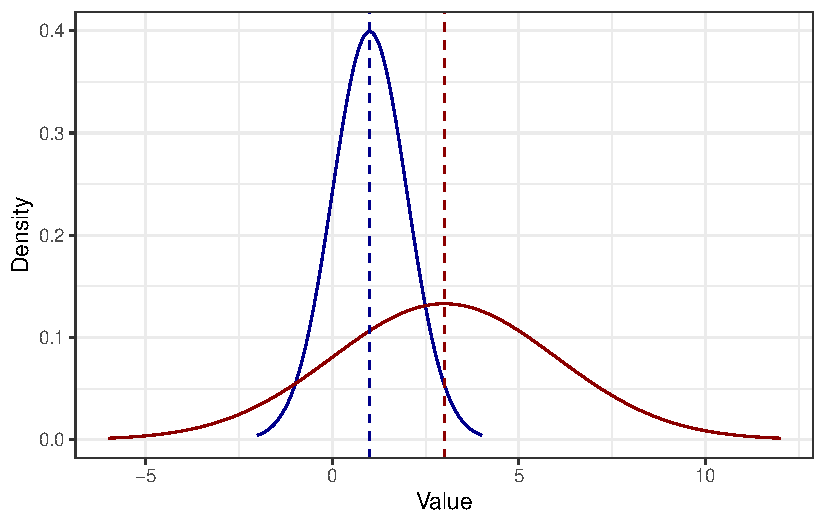
\includegraphics{andan-descriptives_files/figure-pdf/mean_feature_2-1.pdf}

Тут, правда, явно \hyperref[var_features]{что-то ещё} произошло, но мы
пока этого не знаем. Однако, отметит этот факт.

\begin{itemize}
\tightlist
\item
  \textbf{Сумма отклонений от среднего значения равна нулю.}
\end{itemize}

\[
\sum_{i=1}^n(x_i - M_X) = 0
\]

Элегантное доказательство:

\[
\sum_{i=1}^n(x_i - M_X) = \sum_{i=1}^n x_i - \sum_{i=1}^n M_X = \sum_{i=1}^n x_i - nM_X = \\
= \sum_{i=1}^n x_i - n \times \frac{1}{n} \sum_{i=1}^n x_i = \sum_{i=1}^n x_i - \sum_{i=1}^n x_i = 0
\]

Но можно это осмыслить и более просто графически.

\textbf{Отклонение} --- это разность между средним и конкретным
значением переменной. И, действительно, так как среднее находится в
центре распределения, то часть значений лежит справа, а часть слева.
Значит, будут как положительные, так и отрицательные отклонения --- и их
сумма в итоге будет равна нулю.

\begin{verbatim}
Warning in grid.Call.graphics(C_text, as.graphicsAnnot(x$label), x$x, x$y, :
conversion failure on 'отрицательные' in 'mbcsToSbcs': dot substituted for <d0>
\end{verbatim}

\begin{verbatim}
Warning in grid.Call.graphics(C_text, as.graphicsAnnot(x$label), x$x, x$y, :
conversion failure on 'отрицательные' in 'mbcsToSbcs': dot substituted for <be>
\end{verbatim}

\begin{verbatim}
Warning in grid.Call.graphics(C_text, as.graphicsAnnot(x$label), x$x, x$y, :
conversion failure on 'отрицательные' in 'mbcsToSbcs': dot substituted for <d1>
\end{verbatim}

\begin{verbatim}
Warning in grid.Call.graphics(C_text, as.graphicsAnnot(x$label), x$x, x$y, :
conversion failure on 'отрицательные' in 'mbcsToSbcs': dot substituted for <82>
\end{verbatim}

\begin{verbatim}
Warning in grid.Call.graphics(C_text, as.graphicsAnnot(x$label), x$x, x$y, :
conversion failure on 'отрицательные' in 'mbcsToSbcs': dot substituted for <d1>
\end{verbatim}

\begin{verbatim}
Warning in grid.Call.graphics(C_text, as.graphicsAnnot(x$label), x$x, x$y, :
conversion failure on 'отрицательные' in 'mbcsToSbcs': dot substituted for <80>
\end{verbatim}

\begin{verbatim}
Warning in grid.Call.graphics(C_text, as.graphicsAnnot(x$label), x$x, x$y, :
conversion failure on 'отрицательные' in 'mbcsToSbcs': dot substituted for <d0>
\end{verbatim}

\begin{verbatim}
Warning in grid.Call.graphics(C_text, as.graphicsAnnot(x$label), x$x, x$y, :
conversion failure on 'отрицательные' in 'mbcsToSbcs': dot substituted for <b8>
\end{verbatim}

\begin{verbatim}
Warning in grid.Call.graphics(C_text, as.graphicsAnnot(x$label), x$x, x$y, :
conversion failure on 'отрицательные' in 'mbcsToSbcs': dot substituted for <d1>
\end{verbatim}

\begin{verbatim}
Warning in grid.Call.graphics(C_text, as.graphicsAnnot(x$label), x$x, x$y, :
conversion failure on 'отрицательные' in 'mbcsToSbcs': dot substituted for <86>
\end{verbatim}

\begin{verbatim}
Warning in grid.Call.graphics(C_text, as.graphicsAnnot(x$label), x$x, x$y, :
conversion failure on 'отрицательные' in 'mbcsToSbcs': dot substituted for <d0>
\end{verbatim}

\begin{verbatim}
Warning in grid.Call.graphics(C_text, as.graphicsAnnot(x$label), x$x, x$y, :
conversion failure on 'отрицательные' in 'mbcsToSbcs': dot substituted for <b0>
\end{verbatim}

\begin{verbatim}
Warning in grid.Call.graphics(C_text, as.graphicsAnnot(x$label), x$x, x$y, :
conversion failure on 'отрицательные' in 'mbcsToSbcs': dot substituted for <d1>
\end{verbatim}

\begin{verbatim}
Warning in grid.Call.graphics(C_text, as.graphicsAnnot(x$label), x$x, x$y, :
conversion failure on 'отрицательные' in 'mbcsToSbcs': dot substituted for <82>
\end{verbatim}

\begin{verbatim}
Warning in grid.Call.graphics(C_text, as.graphicsAnnot(x$label), x$x, x$y, :
conversion failure on 'отрицательные' in 'mbcsToSbcs': dot substituted for <d0>
\end{verbatim}

\begin{verbatim}
Warning in grid.Call.graphics(C_text, as.graphicsAnnot(x$label), x$x, x$y, :
conversion failure on 'отрицательные' in 'mbcsToSbcs': dot substituted for <b5>
\end{verbatim}

\begin{verbatim}
Warning in grid.Call.graphics(C_text, as.graphicsAnnot(x$label), x$x, x$y, :
conversion failure on 'отрицательные' in 'mbcsToSbcs': dot substituted for <d0>
\end{verbatim}

\begin{verbatim}
Warning in grid.Call.graphics(C_text, as.graphicsAnnot(x$label), x$x, x$y, :
conversion failure on 'отрицательные' in 'mbcsToSbcs': dot substituted for <bb>
\end{verbatim}

\begin{verbatim}
Warning in grid.Call.graphics(C_text, as.graphicsAnnot(x$label), x$x, x$y, :
conversion failure on 'отрицательные' in 'mbcsToSbcs': dot substituted for <d1>
\end{verbatim}

\begin{verbatim}
Warning in grid.Call.graphics(C_text, as.graphicsAnnot(x$label), x$x, x$y, :
conversion failure on 'отрицательные' in 'mbcsToSbcs': dot substituted for <8c>
\end{verbatim}

\begin{verbatim}
Warning in grid.Call.graphics(C_text, as.graphicsAnnot(x$label), x$x, x$y, :
conversion failure on 'отрицательные' in 'mbcsToSbcs': dot substituted for <d0>
\end{verbatim}

\begin{verbatim}
Warning in grid.Call.graphics(C_text, as.graphicsAnnot(x$label), x$x, x$y, :
conversion failure on 'отрицательные' in 'mbcsToSbcs': dot substituted for <bd>
\end{verbatim}

\begin{verbatim}
Warning in grid.Call.graphics(C_text, as.graphicsAnnot(x$label), x$x, x$y, :
conversion failure on 'отрицательные' in 'mbcsToSbcs': dot substituted for <d1>
\end{verbatim}

\begin{verbatim}
Warning in grid.Call.graphics(C_text, as.graphicsAnnot(x$label), x$x, x$y, :
conversion failure on 'отрицательные' in 'mbcsToSbcs': dot substituted for <8b>
\end{verbatim}

\begin{verbatim}
Warning in grid.Call.graphics(C_text, as.graphicsAnnot(x$label), x$x, x$y, :
conversion failure on 'отрицательные' in 'mbcsToSbcs': dot substituted for <d0>
\end{verbatim}

\begin{verbatim}
Warning in grid.Call.graphics(C_text, as.graphicsAnnot(x$label), x$x, x$y, :
conversion failure on 'отрицательные' in 'mbcsToSbcs': dot substituted for <b5>
\end{verbatim}

\begin{verbatim}
Warning in grid.Call.graphics(C_text, as.graphicsAnnot(x$label), x$x, x$y, :
conversion failure on 'отклонения' in 'mbcsToSbcs': dot substituted for <d0>
\end{verbatim}

\begin{verbatim}
Warning in grid.Call.graphics(C_text, as.graphicsAnnot(x$label), x$x, x$y, :
conversion failure on 'отклонения' in 'mbcsToSbcs': dot substituted for <be>
\end{verbatim}

\begin{verbatim}
Warning in grid.Call.graphics(C_text, as.graphicsAnnot(x$label), x$x, x$y, :
conversion failure on 'отклонения' in 'mbcsToSbcs': dot substituted for <d1>
\end{verbatim}

\begin{verbatim}
Warning in grid.Call.graphics(C_text, as.graphicsAnnot(x$label), x$x, x$y, :
conversion failure on 'отклонения' in 'mbcsToSbcs': dot substituted for <82>
\end{verbatim}

\begin{verbatim}
Warning in grid.Call.graphics(C_text, as.graphicsAnnot(x$label), x$x, x$y, :
conversion failure on 'отклонения' in 'mbcsToSbcs': dot substituted for <d0>
\end{verbatim}

\begin{verbatim}
Warning in grid.Call.graphics(C_text, as.graphicsAnnot(x$label), x$x, x$y, :
conversion failure on 'отклонения' in 'mbcsToSbcs': dot substituted for <ba>
\end{verbatim}

\begin{verbatim}
Warning in grid.Call.graphics(C_text, as.graphicsAnnot(x$label), x$x, x$y, :
conversion failure on 'отклонения' in 'mbcsToSbcs': dot substituted for <d0>
\end{verbatim}

\begin{verbatim}
Warning in grid.Call.graphics(C_text, as.graphicsAnnot(x$label), x$x, x$y, :
conversion failure on 'отклонения' in 'mbcsToSbcs': dot substituted for <bb>
\end{verbatim}

\begin{verbatim}
Warning in grid.Call.graphics(C_text, as.graphicsAnnot(x$label), x$x, x$y, :
conversion failure on 'отклонения' in 'mbcsToSbcs': dot substituted for <d0>
\end{verbatim}

\begin{verbatim}
Warning in grid.Call.graphics(C_text, as.graphicsAnnot(x$label), x$x, x$y, :
conversion failure on 'отклонения' in 'mbcsToSbcs': dot substituted for <be>
\end{verbatim}

\begin{verbatim}
Warning in grid.Call.graphics(C_text, as.graphicsAnnot(x$label), x$x, x$y, :
conversion failure on 'отклонения' in 'mbcsToSbcs': dot substituted for <d0>
\end{verbatim}

\begin{verbatim}
Warning in grid.Call.graphics(C_text, as.graphicsAnnot(x$label), x$x, x$y, :
conversion failure on 'отклонения' in 'mbcsToSbcs': dot substituted for <bd>
\end{verbatim}

\begin{verbatim}
Warning in grid.Call.graphics(C_text, as.graphicsAnnot(x$label), x$x, x$y, :
conversion failure on 'отклонения' in 'mbcsToSbcs': dot substituted for <d0>
\end{verbatim}

\begin{verbatim}
Warning in grid.Call.graphics(C_text, as.graphicsAnnot(x$label), x$x, x$y, :
conversion failure on 'отклонения' in 'mbcsToSbcs': dot substituted for <b5>
\end{verbatim}

\begin{verbatim}
Warning in grid.Call.graphics(C_text, as.graphicsAnnot(x$label), x$x, x$y, :
conversion failure on 'отклонения' in 'mbcsToSbcs': dot substituted for <d0>
\end{verbatim}

\begin{verbatim}
Warning in grid.Call.graphics(C_text, as.graphicsAnnot(x$label), x$x, x$y, :
conversion failure on 'отклонения' in 'mbcsToSbcs': dot substituted for <bd>
\end{verbatim}

\begin{verbatim}
Warning in grid.Call.graphics(C_text, as.graphicsAnnot(x$label), x$x, x$y, :
conversion failure on 'отклонения' in 'mbcsToSbcs': dot substituted for <d0>
\end{verbatim}

\begin{verbatim}
Warning in grid.Call.graphics(C_text, as.graphicsAnnot(x$label), x$x, x$y, :
conversion failure on 'отклонения' in 'mbcsToSbcs': dot substituted for <b8>
\end{verbatim}

\begin{verbatim}
Warning in grid.Call.graphics(C_text, as.graphicsAnnot(x$label), x$x, x$y, :
conversion failure on 'отклонения' in 'mbcsToSbcs': dot substituted for <d1>
\end{verbatim}

\begin{verbatim}
Warning in grid.Call.graphics(C_text, as.graphicsAnnot(x$label), x$x, x$y, :
conversion failure on 'отклонения' in 'mbcsToSbcs': dot substituted for <8f>
\end{verbatim}

\begin{verbatim}
Warning in grid.Call.graphics(C_text, as.graphicsAnnot(x$label), x$x, x$y, :
conversion failure on 'положительные' in 'mbcsToSbcs': dot substituted for <d0>
\end{verbatim}

\begin{verbatim}
Warning in grid.Call.graphics(C_text, as.graphicsAnnot(x$label), x$x, x$y, :
conversion failure on 'положительные' in 'mbcsToSbcs': dot substituted for <bf>
\end{verbatim}

\begin{verbatim}
Warning in grid.Call.graphics(C_text, as.graphicsAnnot(x$label), x$x, x$y, :
conversion failure on 'положительные' in 'mbcsToSbcs': dot substituted for <d0>
\end{verbatim}

\begin{verbatim}
Warning in grid.Call.graphics(C_text, as.graphicsAnnot(x$label), x$x, x$y, :
conversion failure on 'положительные' in 'mbcsToSbcs': dot substituted for <be>
\end{verbatim}

\begin{verbatim}
Warning in grid.Call.graphics(C_text, as.graphicsAnnot(x$label), x$x, x$y, :
conversion failure on 'положительные' in 'mbcsToSbcs': dot substituted for <d0>
\end{verbatim}

\begin{verbatim}
Warning in grid.Call.graphics(C_text, as.graphicsAnnot(x$label), x$x, x$y, :
conversion failure on 'положительные' in 'mbcsToSbcs': dot substituted for <bb>
\end{verbatim}

\begin{verbatim}
Warning in grid.Call.graphics(C_text, as.graphicsAnnot(x$label), x$x, x$y, :
conversion failure on 'положительные' in 'mbcsToSbcs': dot substituted for <d0>
\end{verbatim}

\begin{verbatim}
Warning in grid.Call.graphics(C_text, as.graphicsAnnot(x$label), x$x, x$y, :
conversion failure on 'положительные' in 'mbcsToSbcs': dot substituted for <be>
\end{verbatim}

\begin{verbatim}
Warning in grid.Call.graphics(C_text, as.graphicsAnnot(x$label), x$x, x$y, :
conversion failure on 'положительные' in 'mbcsToSbcs': dot substituted for <d0>
\end{verbatim}

\begin{verbatim}
Warning in grid.Call.graphics(C_text, as.graphicsAnnot(x$label), x$x, x$y, :
conversion failure on 'положительные' in 'mbcsToSbcs': dot substituted for <b6>
\end{verbatim}

\begin{verbatim}
Warning in grid.Call.graphics(C_text, as.graphicsAnnot(x$label), x$x, x$y, :
conversion failure on 'положительные' in 'mbcsToSbcs': dot substituted for <d0>
\end{verbatim}

\begin{verbatim}
Warning in grid.Call.graphics(C_text, as.graphicsAnnot(x$label), x$x, x$y, :
conversion failure on 'положительные' in 'mbcsToSbcs': dot substituted for <b8>
\end{verbatim}

\begin{verbatim}
Warning in grid.Call.graphics(C_text, as.graphicsAnnot(x$label), x$x, x$y, :
conversion failure on 'положительные' in 'mbcsToSbcs': dot substituted for <d1>
\end{verbatim}

\begin{verbatim}
Warning in grid.Call.graphics(C_text, as.graphicsAnnot(x$label), x$x, x$y, :
conversion failure on 'положительные' in 'mbcsToSbcs': dot substituted for <82>
\end{verbatim}

\begin{verbatim}
Warning in grid.Call.graphics(C_text, as.graphicsAnnot(x$label), x$x, x$y, :
conversion failure on 'положительные' in 'mbcsToSbcs': dot substituted for <d0>
\end{verbatim}

\begin{verbatim}
Warning in grid.Call.graphics(C_text, as.graphicsAnnot(x$label), x$x, x$y, :
conversion failure on 'положительные' in 'mbcsToSbcs': dot substituted for <b5>
\end{verbatim}

\begin{verbatim}
Warning in grid.Call.graphics(C_text, as.graphicsAnnot(x$label), x$x, x$y, :
conversion failure on 'положительные' in 'mbcsToSbcs': dot substituted for <d0>
\end{verbatim}

\begin{verbatim}
Warning in grid.Call.graphics(C_text, as.graphicsAnnot(x$label), x$x, x$y, :
conversion failure on 'положительные' in 'mbcsToSbcs': dot substituted for <bb>
\end{verbatim}

\begin{verbatim}
Warning in grid.Call.graphics(C_text, as.graphicsAnnot(x$label), x$x, x$y, :
conversion failure on 'положительные' in 'mbcsToSbcs': dot substituted for <d1>
\end{verbatim}

\begin{verbatim}
Warning in grid.Call.graphics(C_text, as.graphicsAnnot(x$label), x$x, x$y, :
conversion failure on 'положительные' in 'mbcsToSbcs': dot substituted for <8c>
\end{verbatim}

\begin{verbatim}
Warning in grid.Call.graphics(C_text, as.graphicsAnnot(x$label), x$x, x$y, :
conversion failure on 'положительные' in 'mbcsToSbcs': dot substituted for <d0>
\end{verbatim}

\begin{verbatim}
Warning in grid.Call.graphics(C_text, as.graphicsAnnot(x$label), x$x, x$y, :
conversion failure on 'положительные' in 'mbcsToSbcs': dot substituted for <bd>
\end{verbatim}

\begin{verbatim}
Warning in grid.Call.graphics(C_text, as.graphicsAnnot(x$label), x$x, x$y, :
conversion failure on 'положительные' in 'mbcsToSbcs': dot substituted for <d1>
\end{verbatim}

\begin{verbatim}
Warning in grid.Call.graphics(C_text, as.graphicsAnnot(x$label), x$x, x$y, :
conversion failure on 'положительные' in 'mbcsToSbcs': dot substituted for <8b>
\end{verbatim}

\begin{verbatim}
Warning in grid.Call.graphics(C_text, as.graphicsAnnot(x$label), x$x, x$y, :
conversion failure on 'положительные' in 'mbcsToSbcs': dot substituted for <d0>
\end{verbatim}

\begin{verbatim}
Warning in grid.Call.graphics(C_text, as.graphicsAnnot(x$label), x$x, x$y, :
conversion failure on 'положительные' in 'mbcsToSbcs': dot substituted for <b5>
\end{verbatim}

\begin{verbatim}
Warning in grid.Call.graphics(C_text, as.graphicsAnnot(x$label), x$x, x$y, :
conversion failure on 'отклонения' in 'mbcsToSbcs': dot substituted for <d0>
\end{verbatim}

\begin{verbatim}
Warning in grid.Call.graphics(C_text, as.graphicsAnnot(x$label), x$x, x$y, :
conversion failure on 'отклонения' in 'mbcsToSbcs': dot substituted for <be>
\end{verbatim}

\begin{verbatim}
Warning in grid.Call.graphics(C_text, as.graphicsAnnot(x$label), x$x, x$y, :
conversion failure on 'отклонения' in 'mbcsToSbcs': dot substituted for <d1>
\end{verbatim}

\begin{verbatim}
Warning in grid.Call.graphics(C_text, as.graphicsAnnot(x$label), x$x, x$y, :
conversion failure on 'отклонения' in 'mbcsToSbcs': dot substituted for <82>
\end{verbatim}

\begin{verbatim}
Warning in grid.Call.graphics(C_text, as.graphicsAnnot(x$label), x$x, x$y, :
conversion failure on 'отклонения' in 'mbcsToSbcs': dot substituted for <d0>
\end{verbatim}

\begin{verbatim}
Warning in grid.Call.graphics(C_text, as.graphicsAnnot(x$label), x$x, x$y, :
conversion failure on 'отклонения' in 'mbcsToSbcs': dot substituted for <ba>
\end{verbatim}

\begin{verbatim}
Warning in grid.Call.graphics(C_text, as.graphicsAnnot(x$label), x$x, x$y, :
conversion failure on 'отклонения' in 'mbcsToSbcs': dot substituted for <d0>
\end{verbatim}

\begin{verbatim}
Warning in grid.Call.graphics(C_text, as.graphicsAnnot(x$label), x$x, x$y, :
conversion failure on 'отклонения' in 'mbcsToSbcs': dot substituted for <bb>
\end{verbatim}

\begin{verbatim}
Warning in grid.Call.graphics(C_text, as.graphicsAnnot(x$label), x$x, x$y, :
conversion failure on 'отклонения' in 'mbcsToSbcs': dot substituted for <d0>
\end{verbatim}

\begin{verbatim}
Warning in grid.Call.graphics(C_text, as.graphicsAnnot(x$label), x$x, x$y, :
conversion failure on 'отклонения' in 'mbcsToSbcs': dot substituted for <be>
\end{verbatim}

\begin{verbatim}
Warning in grid.Call.graphics(C_text, as.graphicsAnnot(x$label), x$x, x$y, :
conversion failure on 'отклонения' in 'mbcsToSbcs': dot substituted for <d0>
\end{verbatim}

\begin{verbatim}
Warning in grid.Call.graphics(C_text, as.graphicsAnnot(x$label), x$x, x$y, :
conversion failure on 'отклонения' in 'mbcsToSbcs': dot substituted for <bd>
\end{verbatim}

\begin{verbatim}
Warning in grid.Call.graphics(C_text, as.graphicsAnnot(x$label), x$x, x$y, :
conversion failure on 'отклонения' in 'mbcsToSbcs': dot substituted for <d0>
\end{verbatim}

\begin{verbatim}
Warning in grid.Call.graphics(C_text, as.graphicsAnnot(x$label), x$x, x$y, :
conversion failure on 'отклонения' in 'mbcsToSbcs': dot substituted for <b5>
\end{verbatim}

\begin{verbatim}
Warning in grid.Call.graphics(C_text, as.graphicsAnnot(x$label), x$x, x$y, :
conversion failure on 'отклонения' in 'mbcsToSbcs': dot substituted for <d0>
\end{verbatim}

\begin{verbatim}
Warning in grid.Call.graphics(C_text, as.graphicsAnnot(x$label), x$x, x$y, :
conversion failure on 'отклонения' in 'mbcsToSbcs': dot substituted for <bd>
\end{verbatim}

\begin{verbatim}
Warning in grid.Call.graphics(C_text, as.graphicsAnnot(x$label), x$x, x$y, :
conversion failure on 'отклонения' in 'mbcsToSbcs': dot substituted for <d0>
\end{verbatim}

\begin{verbatim}
Warning in grid.Call.graphics(C_text, as.graphicsAnnot(x$label), x$x, x$y, :
conversion failure on 'отклонения' in 'mbcsToSbcs': dot substituted for <b8>
\end{verbatim}

\begin{verbatim}
Warning in grid.Call.graphics(C_text, as.graphicsAnnot(x$label), x$x, x$y, :
conversion failure on 'отклонения' in 'mbcsToSbcs': dot substituted for <d1>
\end{verbatim}

\begin{verbatim}
Warning in grid.Call.graphics(C_text, as.graphicsAnnot(x$label), x$x, x$y, :
conversion failure on 'отклонения' in 'mbcsToSbcs': dot substituted for <8f>
\end{verbatim}

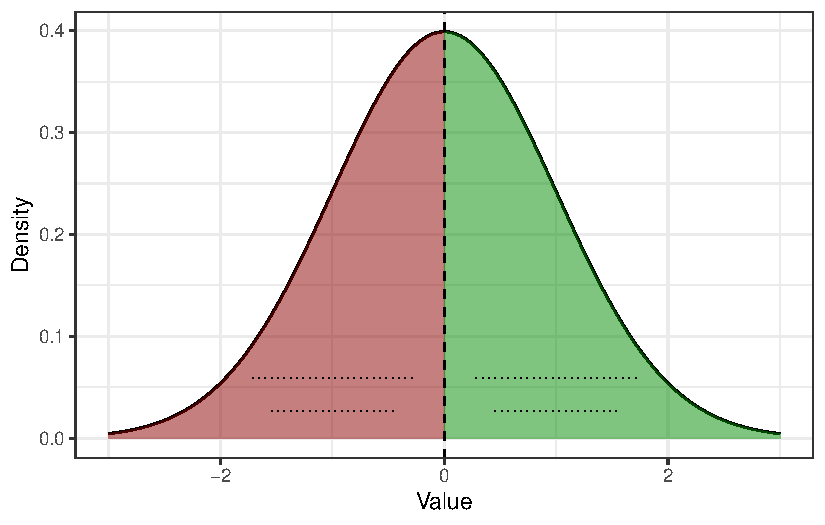
\includegraphics{andan-descriptives_files/figure-pdf/zero_deviation_sum-1.pdf}

\subsubsection{Усеченное среднее}\label{andan-descriptives-trimmed-mean}

ПРО УСЕЧЕННОЕ СРЕДНЕЕ

Среднее арифметическое не одиноко --- есть и другие. Встретяться они вам
примерно нигде --- то есть о-о-о-очень редко и, скорее всего, в каком-то
изощрённом виде. Но упомянуть их, пожалуй, стоит.

\subsubsection{Геометрическое
среднее}\label{andan-descriptives-geometric-mean}

Редко встречается в научных работах, но заради общего представления
пусть будет. Поскольку оно считается через умножение, то может быть
рассчитано только на абсолютной шкале.

\[
G_{X} = \sqrt[n]{\prod_{i=1}^n x_i} = \Big(\prod_{i=1}^n x_i\Big)^{\tfrac{1}{n}}
\]

\subsubsection{Квадратичное
среднее}\label{andan-descriptives-quandratic-mean}

\begin{quote}
А вот это уже более полезная история. Мы с ним столкнёмся далее, правда
под разными масками.
\end{quote}

\textbf{Квадратичное среднее (quadratic mean, root mean square, RMS)}
--- это квадратный корень из среднего квадрата наблюдений. Ничего не
понятно, поэтому по порядку.

\begin{itemize}
\tightlist
\item
  есть наблюдение \(x_i\)
\item
  значит есть и его квадрат \(x_i^2\)
\item
  мы умеем считать обычно среднее арифметическое, но ведь \(x_i^2\) ---
  это тоже наблюдение, просто в квадрате, так?
\item
  значит можем посчитать среднее арифметическое квадратов наблюдений ---
  \emph{средний квадрат}
\end{itemize}

\[
\frac{\sum_{i=1}^n x_i^2}{n}
\]

\begin{itemize}
\tightlist
\item
  норм, а теперь извлечём из этого дела корень --- получим то, что там
  надо
\end{itemize}

\[
X_{\mathrm{RMS}} = \sqrt{\frac{\sum_{i=1}^n x_i^2}{n}}
\]

Per se\footnote{Per se (лат.) --- «само по себе», «как таковое», «в
  чистом виде».} мы его вряд ли ещё когда-то увидим, но пару раз оно
внезапно всплывет.

\subsubsection{Гармоническое
среднее}\label{andan-descriptives-harmonic-mean}

\begin{quote}
Суперэкзотичный покемон.
\end{quote}

\[
H_X = \frac{n \prod_{i=1}^n x_i}{\sum_{i=1}^n (\tfrac{1}{x} \prod_{j=1}^n x_j)} = \frac{n}{\sum_{i=1}^n \tfrac{1}{x_i}}
\]

\subsubsection{Взвешенное
среднее}\label{andan-descriptives-weighted-mean}

Часто бывает такая ситуация, что нас нужно посчитать среднее по
каким-либо имеющимся параметрам, но одни параметры для нас важнее, чем
другие. Например, мы хотим вычислить суммарный балл обучающегося за курс
на основе ряда работ, выполненных в течение курса, однако мы понимаем,
что тест из десяти вопросов с множественном выбором явно менее
показателен, чем, например, аналитическое эссе или экзаменационная
оценка. Что делать? Взвесить параметры!

Что значит взвесить? Умножить на некоторое число. На самом деле, любое.
Пусть мы посчитали, что написать эссе в три абстрактных раза тяжелее,
чем написать тест, а сдать экзамен в два раза тяжелее, чем написать
эссе. Тогда мы можем присвоить баллу за тест вес \(1\), баллу за
аналитическое эссе вес \(3\), а экзамену --- вес \(6\). Тогда итоговая
оценка за курс будет рассчитываться следующим образом:

\[
\text{final score } = 1 \cdot \text{test} + 3 \cdot \text{essay} + 6 \cdot \text{exam}
\]

Суперкласс. Однако! Весьма вероятно, что в учебном заведении принята
единая система оценки для всех видов работ (ну, скажем, некая
абстрактная десятибалльная система в сферическом вакууме). Получается,
если и за тест, и за эссе, и за экзамен у студента по 10 баллов, то
суммарный балл 100, что, кажется, больше, чем 10. Чтобы вернуться к
изначальным границам баллов, нужно моделить суммарный балл на сумму
весов параметров:

\[
\text{final score } = \frac{1 \cdot \text{test} + 3 \cdot \text{essay} + 6 \cdot \text{exam}}{1 + 3 + 6}
\]

Кайф! Собственно, это и есть взвешенное среднее. Коэффициенты, на
которые мы умножаем значение парамернов, называются \emph{весами
параметров}. И в общем виде формула принимает следующий вид.

\[
\bar x = \frac{\sum_{i=1}^n w_i x_i}{\sum_{i=1}^n w_i} = \sum_{i=1}^n w_i' x_i,
\]

где \(x_i\) --- значения конкретных параметров, \(w_i\) --- веса
конкретных параметров, \(w_i'\) --- нормированные веса параметров.

Вторая часть формулы показывается нам, что можно облегчить себе
вычислительную жизнь, если заранее нормировать веса, то есть разделить
каждый коэффициент на сумму коэффициентов:

\[
w_i' = \frac{w_i}{\sum_{i=1}^n w_i}
\]

Тогда сумма коэффициентов будет равна единице. Так чаще всего и
поступают, так как тогда коэффициент будет представлять долю, которую
весит данный параметр в суммарной оценке. Удобно, практично, красиво.

Взвещенное среднее часто применяется именно во всякого рода
ассессментах, и не только образовательных. Например, вы HR-аналитик и
оцениваете персонал. Вы аналитически вычисляете веса коэффициентов
(допустим, с помощью линейной регрессии), а далее на их основе
высчитаете интегральный балл, по которому будете оценивать сотрудников.
Это как один из индустриальных примеров.

Также оно применяется, когда в наших данных есть какая-то группировка
(например, когорты), при этом группы неравномерны.

\subsection{Среднее vs медиана}\label{andan-descriptives-mean-vs-median}

Помимо того, что среднее и медиана информативны сами по себе, полезно
смотреть на их взаимное расположение.

\begin{quote}
Сравнивать будем моду, медиану и среднее {[}арифметическое{]}.
\end{quote}

Итак, все три статистики --- мода, медиана и среднее --- описывают
центральную тенденцию --- некоторое значение изучаемой нами переменной,
вокруг которого собираются другие значения. Но если их три и все они
используются, значит между ними должны быть какие-то различия.
Посмотрим, какие.

Во-первых, очевидно, что \emph{моду невозможно посчитать для непрерывной
переменной}.

\emph{Нет, не очевидно}

Так как вероятность того, что непрерывная случайная величина принимает
своё конкретное значение, равна нулю, каждое наблюдение в нашей выборке
будет уникально --- встретится ровно \emph{один раз}. Вспомните
{[}посмотрите{]} пример из предыдущей главы, где мы набирали числа из
отрезка. Получается, что мода теряет свой смысл.

Во-вторых, \emph{медиану нельзя посчитать на номинальной шкале}. Кстати,
почему?

\emph{Потому что}

на номинальной шкале нет отношения порядка между элементами. Помните, на
ней нельзя сравнивать на больше-меньше. Поэтому невозможно отсортировать
наблюдения, а значит, и найти медиану.

В-третьих, \emph{среднее тоже нельзя посчитать на номинальной шкале}.

\emph{Можно, но осторожно}

Вообще, конечно, да --- нельзя, потому что на номинальной шкале не
определена операция сложения, входящая в вычисление среднего. Однако
если на номинальной шкале есть только \emph{две категории}, которые
закодированы \texttt{0} и \texttt{1}, то посчитать среднее можно. Но что
оно будет значить?

Исходный математический смысл среднего явно утерян. Посмотрим на это
по-другому: посчитать сумму единиц это всё равно, что посчитать
\emph{количество} единиц. То есть, если мы сложим все нули и единицы, то
получим количество единиц среди всех наших наблюдений. А разделив
количество единиц на количество наблюдений, мы получим \emph{долю
единиц} --- то есть долю наблюдений с лейблом \texttt{1}.

Вот так вот.

В-четвертых, \emph{для дискретной переменной значение среднего
арифметического будет не особо осмысленно.} Ну, скажем, странно сказать,
что в аудитории в среднем стоят 15.86 столов или в российских семьях в
среднем 1.5 ребенка. Конечно, в ряде случаев можно это как-то
более-менее водержательно интерпретировать, но это требует усилий, а мы
ленивые, поэтому лучше использовать медиану.

\textbf{Итого, делаем следующие выводы}:

\begin{itemize}
\tightlist
\item
  для номинальной шкалы пригодна только мода
\item
  для дискретных переменных подходят мода и медиана

  \begin{itemize}
  \tightlist
  \item
    мода иногда лучше, так как точно всегда будет целым числом
  \end{itemize}
\item
  для непрерывных переменных подходят медиана и среднее
\end{itemize}

Теперь нам надо разобраться, как будут себя вести меры центральной
тенденции в зависимости от \emph{формы распределения}.

\textbf{На симметричном распределении мода, медиана и среднее совпадают}
{[}или, по крайней мере, находятся очень близко друг к другу{]}. Здесь и
далее: красная линия --- среднее, синяя --- медиана, зелёная --- мода.

\begin{verbatim}
Warning: The dot-dot notation (`..density..`) was deprecated in ggplot2 3.4.0.
i Please use `after_stat(density)` instead.
\end{verbatim}

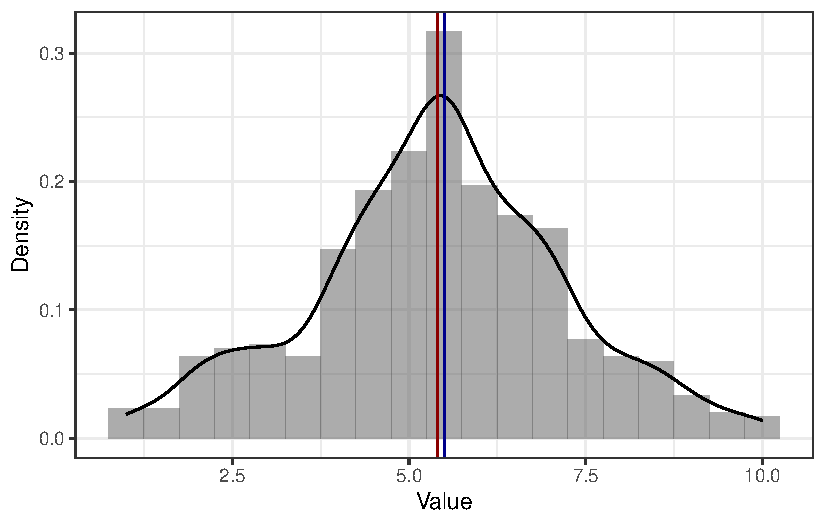
\includegraphics{andan-descriptives_files/figure-pdf/central_tendency_symm-1.pdf}

\textbf{На асимметричном распределении мода {[}практически{]} в пике.}
Практически, потому что функция плотности вероятности {[}черная линия на
графике{]} на всегда точно аппроксимирует (в данном случае то же, что и
сглаживает) эмпирическое распределение. На картинке ниже мы видим, что
на гистограмме мода --- самый высокий столбик, что и показывает нам
зелёная линия, которой обозначена мода. Однако при сглаживании
гистограммы пик немного съехал, и мода оказалась не совсем в вершине
графика функции плотности вероятности.

Вообще-то это нормально, потому что мода для непрерывной величины,
которую мы и визуализируем с помощью графика плотности, либо не может
быть посчитана вовсе, либо --- если так получилось, и у нас все же есть
повторяющиеся значения --- не слишком хорошая мера центральной
тенденции. В целом, и на симметричном распределении мода тоже может
находиться немного в стороне от пика.

\textbf{На асимметричном распределении медиана и среднее смещены в
сторону хвоста. Среднее смещено сильнее медианы.} Это связано с тем, что
медиана зависит только от количества наблюдений, а среднее ещё и от
самих значений. На картинке ниже пример для распределения с
\emph{правосторонней} асимметрии (потому что хвост справа) --- среднее
(красная линия) \emph{правее} медианы (синяя линия).

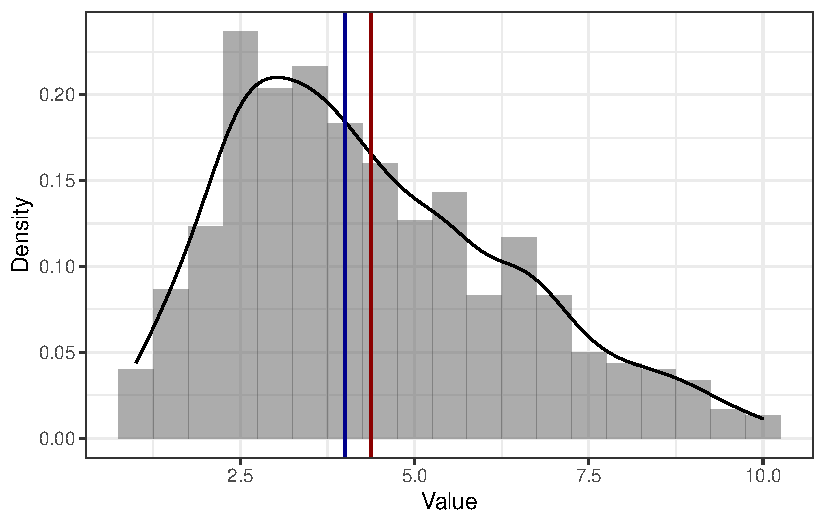
\includegraphics{andan-descriptives_files/figure-pdf/central_tendency_asymm_right-1.pdf}

А это пример для распределения с \emph{левосторонней} асимметрией (так
как хвост слева) --- среднее (красная линия) \emph{левее} медианы (синяя
линия).

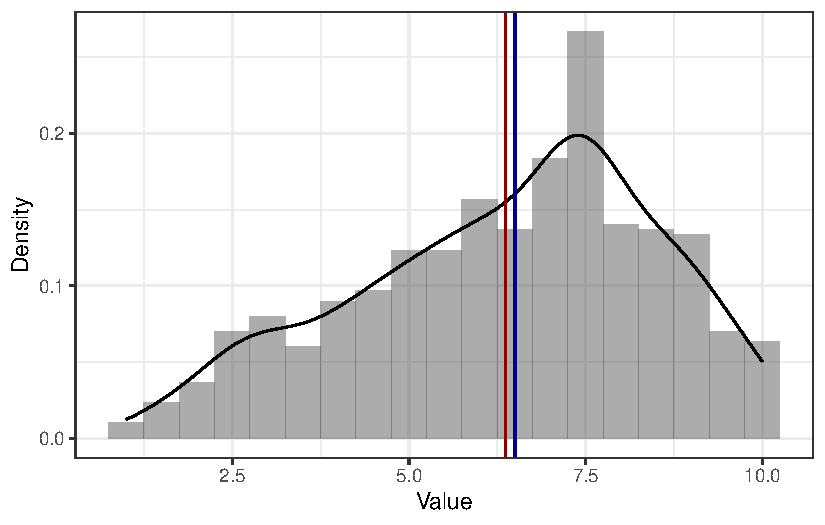
\includegraphics{andan-descriptives_files/figure-pdf/central_tendency_asymm_left-1.pdf}

Для того, чтобы лучше разобраться с тем, как большие и малые значения
влияют на моду и медиану посмотрим такой пример. Пусть у нас есть оценки
за выпускную квалификационную работу. Например, такие:

\begin{Shaded}
\begin{Highlighting}[]
\NormalTok{marks}
\end{Highlighting}
\end{Shaded}

\begin{verbatim}
[1] 6 7 7 8 8
\end{verbatim}

Посчитаем медиану и среднее:

\begin{Shaded}
\begin{Highlighting}[]
\FunctionTok{median}\NormalTok{(marks)}
\end{Highlighting}
\end{Shaded}

\begin{verbatim}
[1] 7
\end{verbatim}

\begin{Shaded}
\begin{Highlighting}[]
\FunctionTok{mean}\NormalTok{(marks)}
\end{Highlighting}
\end{Shaded}

\begin{verbatim}
[1] 7.2
\end{verbatim}

Среднее \(7.2\) округлиться до \(7\), то есть можно считать, что среднее
и медиана совпали. Ну, ок.

Но в комиссии сидят два требовательных доктора наук, которые поставили
оценки, сильно отличающиеся от остальных:

\begin{Shaded}
\begin{Highlighting}[]
\NormalTok{marks}
\end{Highlighting}
\end{Shaded}

\begin{verbatim}
[1] 6 7 7 8 8 3 4
\end{verbatim}

Посчитаем медиану и среднее теперь:

\begin{Shaded}
\begin{Highlighting}[]
\FunctionTok{median}\NormalTok{(marks)}
\end{Highlighting}
\end{Shaded}

\begin{verbatim}
[1] 7
\end{verbatim}

\begin{Shaded}
\begin{Highlighting}[]
\FunctionTok{mean}\NormalTok{(marks)}
\end{Highlighting}
\end{Shaded}

\begin{verbatim}
[1] 6.142857
\end{verbatim}

Медиана осталась на месте --- всё ещё \(7\). А вот среднее \(6.1\)
округлится до \(6\). Казалось бы, это немного, но в смысле оценок ---
это прилично, и может сильно повлиять на GPA.

Итого, среднее более чувствительно к нетипичным значениям (очень большим
или очень малым).

Есть ещё один интересный вариант распределений --- \textbf{бимодальные}.
Значит ли, что у этого распределения две моды? Не всегда. Посмотрим
пример ниже:

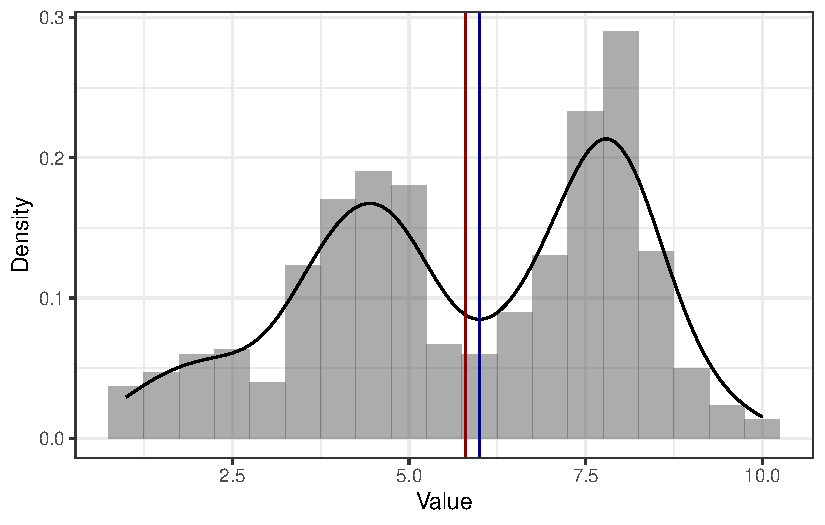
\includegraphics{andan-descriptives_files/figure-pdf/central_tendency_bimodal-1.pdf}

Мы видим, что на графике есть два пика, однако строго математически мода
одна (зеленая линия) --- и она в более высоком пике. Это логично, ибо
там самые часто встречающиеся значения.

И все жё содержательно мы не можем пренебречь вторым пиком. Почему нам
он важен? Обычно бимодальное распределение --- это повод задуматься о
том, что наша выборка неоднородна. \emph{Бимодальное распределение как
бы сложено из двух с центрами в двух пиках.} То есть в нашей выборке как
будто бы \emph{две подвыборки}, которые обладают разными распределениями
интересующего нам признака.

Что с этим делать? Хорошо всегда иметь в данным какие-либо
дополнительные переменные --- как минимум соцдем --- чтобы мы могли по
данным попытаться предположить, какую группировку мы могли забыть учесть
при планировании исследования.

Со средним и медианой происходит примерно то же, что и в случае
асимметричного распределения. Второй пик смещает к себе обе меры
центральной тенденции, причем среднее вновь сильнее, чем медиану.

\section{Меры разброса}\label{andan-descriptives-variability}

Итак, мы разобрались с мерами центральной тенденции. Однако для описания
распределения их оказвается недостаточно. Почему?

\section{Зачем нужны меры разброса}\label{why_we_need_variation}

Посмотрим на несколько распределений:

\begin{Shaded}
\begin{Highlighting}[]
\FunctionTok{set.seed}\NormalTok{(}\DecValTok{123}\NormalTok{)}
\FunctionTok{tibble}\NormalTok{(}\AttributeTok{id =} \DecValTok{1}\SpecialCharTok{:}\DecValTok{100}\NormalTok{,}
       \AttributeTok{x1 =} \FunctionTok{rnorm}\NormalTok{(}\DecValTok{100}\NormalTok{, }\AttributeTok{mean =} \DecValTok{2}\NormalTok{, }\AttributeTok{sd =} \DecValTok{1}\NormalTok{),}
       \AttributeTok{x2 =} \FunctionTok{rnorm}\NormalTok{(}\DecValTok{100}\NormalTok{, }\AttributeTok{mean =} \DecValTok{2}\NormalTok{, }\AttributeTok{sd =} \DecValTok{3}\NormalTok{),}
       \AttributeTok{x3 =} \FunctionTok{rnorm}\NormalTok{(}\DecValTok{100}\NormalTok{, }\AttributeTok{mean =} \DecValTok{2}\NormalTok{, }\AttributeTok{sd =} \FloatTok{0.5}\NormalTok{)) }\OtherTok{{-}\textgreater{}}\NormalTok{ rnorm\_three}
\end{Highlighting}
\end{Shaded}

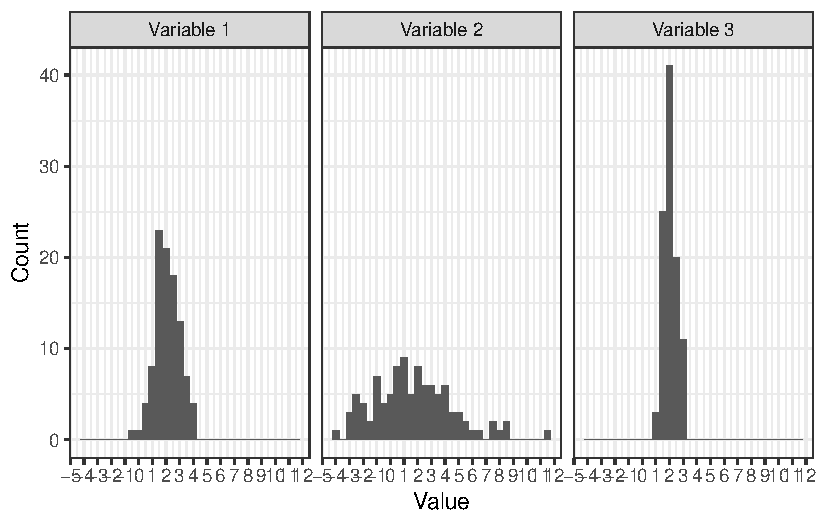
\includegraphics{andan-descriptives_files/figure-pdf/distributions_with_the_same_means_vis-1.pdf}

Методом пристального взгляда можно установить, что у всех распределений
одинаковые средние:

\begin{verbatim}
Warning: Using `size` aesthetic for lines was deprecated in ggplot2 3.4.0.
i Please use `linewidth` instead.
\end{verbatim}

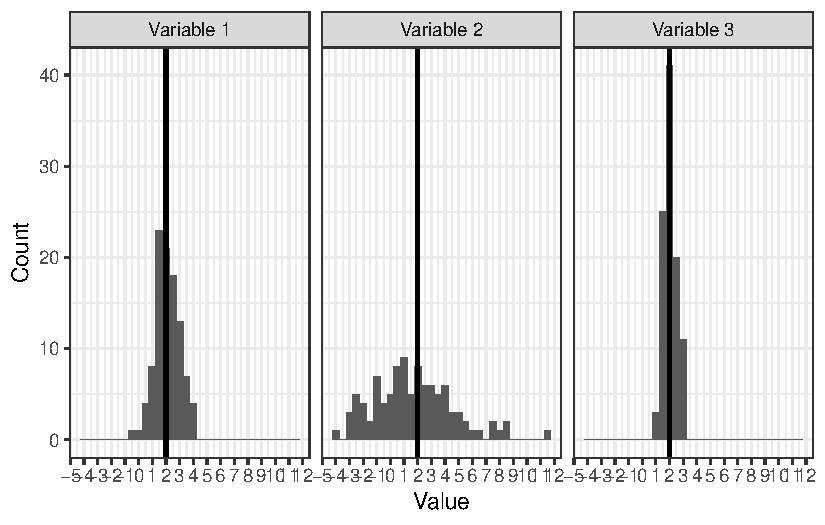
\includegraphics{andan-descriptives_files/figure-pdf/distributions_with_the_same_means_mean-1.pdf}

Однако мы видим, что значения по-разному группируются вокруг среднего.
Как они группируются --- плотно, как на третьем рисунке, или не особо,
как на втором --- можно описать с помощью \textbf{мер разброса}, или
\textbf{мер вариативности}.

\subsection{Основные характеристики статистических
данных}\label{key_features_of_data}

Вообще если посмотреть на это более свысока, то необходимость описания
разброса определяется тем, что статистические данные обладают двумя
ключевыми особенностями --- \emph{неопределенностью} и
\emph{вариативностью}.

\begin{itemize}
\tightlist
\item
  \textbf{Неопределённость} нам говорит о том, что мы не знаем, что
  именно мы получим в результате наших измерений для конкретной выборки.
  В том числе потому, что мы работаем на просторах случайных величин.
\item
  \textbf{Вариативность} означает, что наши данные будут различатся ещё
  и от респондента к респонденту. И между выборками тоже. Здесь и ошибка
  измерения, и различные смешения и ещё куча всего.
\end{itemize}

Более того, вариативность настолько важна, что она входит в расчёт
любого статистического критерия. Именно вариативность --- а не
центральная тенденция --- позволяет нам сделать вывод о том, что наши
выборки различаются (или нет).

\subsection{Минимум, максимум, размах}\label{andan-descriptives-range}

Начнем с самого простого. Как наиболее просто описать вариативность? Мы
работаем с выборкой, а в выборке, как известно, ограниченное число
наблюдений. А если оно ограниченое, значит среди них точно есть
наибольшее --- \emph{максимальное} --- и наименьшее ---
\emph{минимальное}.

Допустим, мы открыли ведомость по «Анатомии и физиологии ЦНС» некоторой
академической группы и пронаблюли следующее:

\begin{Shaded}
\begin{Highlighting}[]
\NormalTok{anat\_marks}
\end{Highlighting}
\end{Shaded}

\begin{verbatim}
 [1]  7  4  6  9 10  5  6  9  6  6  3  6  8  8  5 10  7  5  7  3  9  4  8  3  8
[26]  4  6  8  7  5
\end{verbatim}

Мы можем посчитать минимальное и максимальне значение по этому ряду
наблюдений:

\begin{Shaded}
\begin{Highlighting}[]
\FunctionTok{min}\NormalTok{(anat\_marks)}
\end{Highlighting}
\end{Shaded}

\begin{verbatim}
[1] 3
\end{verbatim}

\begin{Shaded}
\begin{Highlighting}[]
\FunctionTok{max}\NormalTok{(anat\_marks)}
\end{Highlighting}
\end{Shaded}

\begin{verbatim}
[1] 10
\end{verbatim}

Получается, что оценки варьируются от \(3\) до \(10\). Ну, приемлемо.
Разница между максимальным и минимальным значением называется
\textbf{размах (range)}:

\[
\mathrm{range}(X) = \max(X) - \min(X)
\]

Правда вот функция \texttt{range} в \texttt{R} вернёт не само значение
размаха, а минимальное и максимальное значение. Ну, ладно.

\begin{Shaded}
\begin{Highlighting}[]
\FunctionTok{range}\NormalTok{(anat\_marks)}
\end{Highlighting}
\end{Shaded}

\begin{verbatim}
[1]  3 10
\end{verbatim}

И вот мы преисполнившиеся идёт описывать вариативность переменной с
помощью размаха, но обнаруживаем в другой ведомости этой же группы (по
«Введению в психологию») вот что:

\begin{Shaded}
\begin{Highlighting}[]
\NormalTok{intro\_psy\_marks}
\end{Highlighting}
\end{Shaded}

\begin{verbatim}
 [1]  6  8  4  6  7  5  7 10  4  6  7  8  7  6  8 10  8  7  7  6  8  7  6  8  6
[26]  3  8  6  6  4
\end{verbatim}

Размах вроде как такой же:

\begin{Shaded}
\begin{Highlighting}[]
\FunctionTok{range}\NormalTok{(intro\_psy\_marks)}
\end{Highlighting}
\end{Shaded}

\begin{verbatim}
[1]  3 10
\end{verbatim}

Значит ли это, что вариативность одинаковая?

Нарисуем.

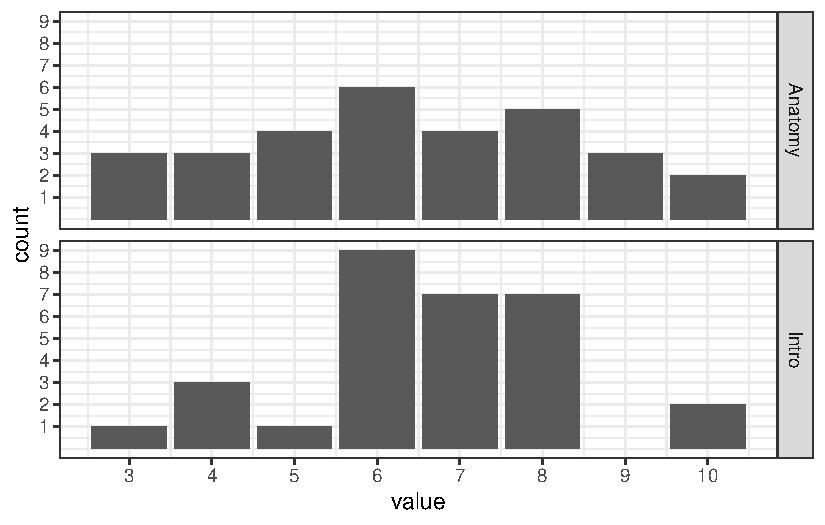
\includegraphics{andan-descriptives_files/figure-pdf/range_problem-1.pdf}

Кажется, что вариативность различна. Распределение оценок по «Анатомии и
физиологии ЦНС» более равномерное, в то время как оценки по «Введению в
психологию» активнее группируются где-то в середине.

Штош, размах хоть и дает нам некоторую информацию о вариативности, нам
этого маловато. Будем искать другие меры разброса.

\subsection{Среднее абсолютное
отклонение}\label{andan-descriptives-average-absolute-deviation}

\subsubsection{Среднее абсолютное отклонение от
среднего}\label{andan-descriptives-mean-absolute-deviation-around-the-mean}

\subsubsection{Среднее абсолютное отклонение от
медианы}\label{andan-descriptives-mean-absolute-deviation-around-the-median}

\subsubsection{Медианное абсолютное
отклонение}\label{andan-descriptives-median-absolute-deviation}

\subsection{Дисперсия}\label{andan-descriptives-variance}

Хотя описание разброса переменных с помощью квантилей (в частности,
квартилей) может дать нам много полезной информации, все же у них есть
существенный недостаток: они никак не взаимодействуют с самими
значениями нашей переменной.

Действительно, мы делим нашу сортированную выборку на равные части, и
смотрим, что в эти части попало. Но хотелось бы как-то учесть ещё и сами
значения переменной в некотрой числовой мере разброса.

Ну, хорошо. Поступим следующим образом. Мы все ещё хотим узнать, как
наши значения группируются вокруг среднего. В предыдущей главе мы уже
видели, что наши наблюдения отклоняются от среднего значения --- значит
мы можем посчитать отклонение для каждого наблюдения:

\[
\bar x - x_i
\]

Окей. Если мы сложим все отклоненияи и поделим на их количество (которое
равно количеству наблюдений), то мы получим среднее отклонение, да?

\[
\frac{1}{n} \sum_{i=1}^n \bar x - x_i
\]

Да. Однако есть одна проблема. В прошлой главе мы
\hyperref[mean_features]{выяснили}, что сумма отклонений от среднего
равна нулю, а значит и среднее отклонение также будет равно нулю.

Хорошо. Но отрицательные значения ведь можно победить! Есть два пути:

\begin{itemize}
\tightlist
\item
  \textbf{Модуль.} Преимущество первого в том, что размерность величины
  разброса остается той же, что и у измеряемой переменной.
\item
  \textbf{Квадрат.} Преимущество второго в том, что сильные отклонения
  будут оказывать более сильное влияние на окончательное значение
  статистики, в то время как для первого малые и большие отклонения
  равноценны.
\end{itemize}

Второй путь на практике оказывается полезнее, так как мы хотим, чтобы
сильно отличающиеся наблюдения вносили вклад в меру разброса.

Возведя отклонения в квадрат, получим формулу \textbf{дисперсии
(вариации, variation)}:

\[
D(X) = \mathrm{var}(X) = \sigma^2 = \frac{1}{n} \sum_{i=1}^n (\bar x - x_i)^2
\]

Гениально.

Не совсем. Формула, которую мы получили, пригодна для расчета
\textbf{дисперсии генеральной совокупности} --- на выборке же она будет
давать неточную оценку.

Чтобы получить точную (несмещенную) оценку \textbf{дисперсии по
выборке}, нам нужно исправить знаменатель дроби --- вместо \(n\)
использовать \(n-1\):

\[
s^2 = \frac{1}{n-1} \sum_{i=1}^n (\bar x - x_i)^2
\]

Но почему?

\subsubsection{Степени свободы}\label{andan-descriptives-df}

Во всём виновата выборка.

Взглянем на формулу дисперсии: в неё входит среднее арифметическое. То
есть для того, чтобы рассчитать дисперсию на выборке, \emph{сначала} нам
необходимо \emph{на этой же выборке} рассчитать среднее. Тем самым, мы
как бы «фиксируем» нашу выборку этим средним значением --- у значений
нашего распределения становится меньше свободы для варьирования. Теперь
свободно варьироваться могут \(n-1\) наблюдение, так как последнее
всегда будет возможно высчитать, исходя из среднего значения. По этой
причине нам необходимо корректировать исходную формулу расчета
дисперсии.

А что если не корректировать?

Мы стремимся к тому, чтобы наши расчеты на выборке достаточно точно
{[}на столько, на сколько это возможно{]} отражали то, что происходит в
генеральной совокупности. Математики-статистики выяснили, что та оценка,
которая хорошо подходит для расчета дисперсии генеральной совокупности,
при применении на выборке даёт \emph{смещенные} оценки. То есть оценка
выборочной дисперсии по формуле дисперсии для генеральной совокупности
содержит в себе \emph{смещение} --- некоторую систематическую ошибку.
Это нехорошо.

К концепту степеней свободы мы ещё неоднократно вернемся. Сейчас
хотелось бы, чтобы сформировалось какое-то минимальное более-менее
освязаемое понимание того, почему они вообще нам нужны. Если на основе
предыдущих абзацев раздела этого сделать не получилось, то давайте
попробуеи воспользоваться следующим рассуждением.

На выборке происходят некоторые статистические преколы, которые
несколько портят нам жизнь, и нам их неободимо учесть, чтобы адекватно
оценивать то, что происходит в генеральной совокупности. В частности,
нам необходимо учитывать количество степеней свободы, которое есть в
нашей выборке. Для расчета выборочной дисперсии оно равно \(n-1\), так
как мы для того, чтобы рассчитать дисперсию по выборке, нам сначала
\emph{по той же самой выборке} надо рассчитать \emph{ещё одну} оценку
--- среднее арифметическое. Этот расчет заберет одну степень свободы у
нашей выборки.

\subsubsection{Дисперсия генеральной
совокупности}\label{andan-descriptives-population-variance}

\subsubsection{Дисперсия
выборки}\label{andan-descriptives-sample-variance}

\subsection{Стандартное
отклонение}\label{andan-descriptives-standard-deviation}

И вот мы получили невероятное! У нас есть формула расчета меры разброса,
которая позволяет учесть сами значения переменной! Ну не чудо ли!

Чудо, конечно, однако есть некоторая проблема. Мы возводили отклонения в
квадрат. Представим, что мы хотим посчитатить дисперсию роста студентов
психфака. Пусть мы измеряли рост в метрах. Отклонения тоже будут в
метрах (потому что среднее --- это тоже метры, а если из метров вычитать
метры, то мы получим метры). А при возведении метров в квадрат
получаются метры в квадрате. Очевидно, что если мы модели квадратные
метры на некоторое число (\(n\)), они все еще останутся метрами в
квадрате.

О, нет! А счастье было так близко, так возможно! Получается, мы не можем
интерпретировать эту меру разброса? Не сможем даже нарисовать?

Да, но это не очень большая беда. Для того, чтобы вернуться обратно к
единицам измерения нашей переменной, нам всего лишь нужно извлечь корень
из дисперсии:

\[
\sigma = \sqrt{\sigma^2} = \sqrt{\frac{1}{n} \sum_{i=1}^n (\bar x - x_i)^2}
\]

Мы получили величину, называемую \textbf{стандартным отклонением
(standard deviation)}. Чем она хороша? Тем, что её размерность совпадает
с размерностью нашей переменной. Стандартное отклонение уже может быть
достаточно интерпретабельно и хорошо визуализируемо.

Кстати, формула выше, которая \hyperref[quadratic_mean]{что-то очень
напоминает}, --- это \textbf{стандартное отклонение генеральной
совокупности}, потому что под корнем стоит дисперсия генеральной
совокупности.

Чтобы посчитать \textbf{стандартное отклонение по выборке}, нам надо
извлечь корень из выборочной дисперсии:

\[
s = \sqrt{s^2} = \sqrt{\frac{1}{n-1} \sum_{i=1}^n (\bar x - x_i)^2}
\]

\subsection{Свойства дисперсии и стандартного
отклонения}\label{andan_descriptives_var_features}

\begin{itemize}
\tightlist
\item
  \textbf{Если к каждому значению распределения прибавить некоторое
  число (константу), то дисперсия не изменится.}
\end{itemize}

\[
D_{x+c} = D_{x}
\]

Вот почему:

\[
D_{x+c} = \frac{\sum_{i=1}^n \big((\bar x + c) - (x_i + c)\big)^2}{n-1} = \frac{\sum_{i=1}^n \big(\bar x + c - x_i - c\big)^2}{n-1} = \frac{\sum_{i=1}^n \big(\bar x - x_i\big)^2}{n-1} = D_x
\]

\begin{itemize}
\tightlist
\item
  \textbf{Если каждое значение распределение умножить на некоторое число
  (константу), то дисперсия увеличится в} \(c^2\) \textbf{раз.}
\end{itemize}

\[
D_{x \times c} = D_{x} \times c^2
\]

Вот почему:

\[
D_{x \times c} = \frac{\sum_{i=1}^n (c\bar x - cx_i)^2}{n-1} = \frac{\sum_{i=1}^n c^2(\bar x - x_i)^2}{n-1} = \frac{c^2 \sum_{i=1}^n (\bar x - x_i)^2}{n-1} = D_x \times c^2
\]

\begin{itemize}
\tightlist
\item
  \textbf{Если к каждому значению распределения прибавить некоторое
  число (константу), то стандартное отклонение не изменится.}
\end{itemize}

\[
s_{x+c} = s_x
\]

Это следует из свойства дисперсии:

\[
s_{x+c} = \sqrt{D_{x+c}} = \sqrt{D_x} = s_x
\]

Как мы уже видели, распределение просто сдвигается на константу.
Например, если к каждому значению синего распределения прибавить \(2\),
получится красное --- разброс у обоих распределений одинаковый:

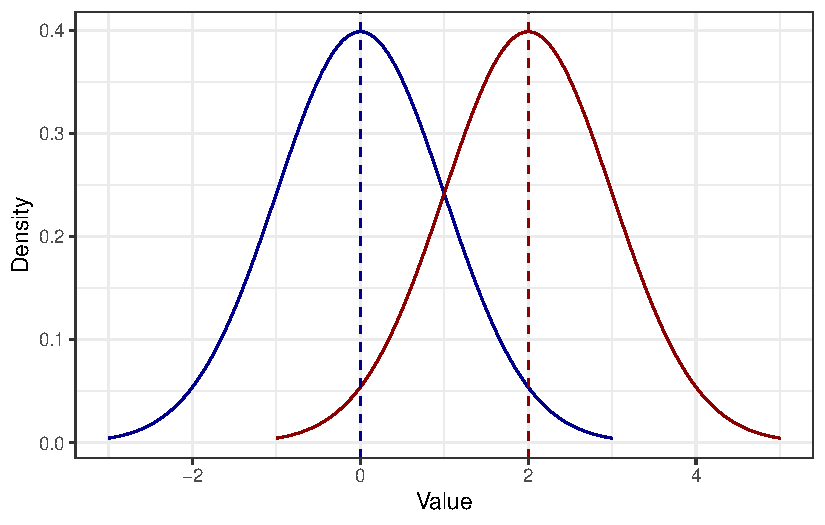
\includegraphics{andan-descriptives_files/figure-pdf/sd_feature_1-1.pdf}

\begin{itemize}
\tightlist
\item
  \textbf{Если каждое значение распределение умножить на некоторое число
  (константу), то стандартное отклонение увеличится во столько же раз.}
\end{itemize}

\[
s_{x \times c} = s_x \times c
\]

Это также следует из свойства дисперсии:

\[
s_{x \times c} = \sqrt{D_{x \times c}} = \sqrt{D_x \times c^2} = s_x \times c
\]

Например, здесь каждое значение синего распределения умножили на \(3\) и
получили красное --- разброс также увеличился в три раза, поэтому
распределение более плоское:

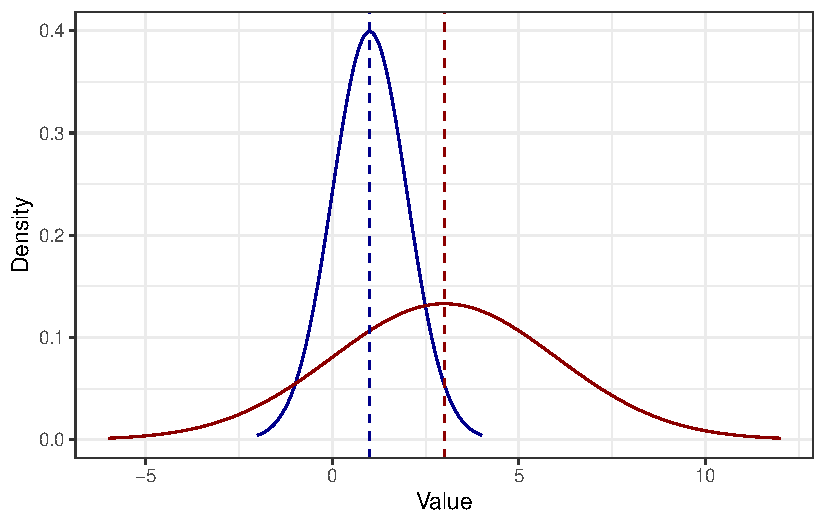
\includegraphics{andan-descriptives_files/figure-pdf/sd_feature_2-1.pdf}

\subsection{Квантили}\label{andan-descriptives-quantiles}

\section{Квантили}\label{quantiles}

Возьмем распределение суммарного балла по шкале «Доверие к техническим
интеллектуальным системам». Выглядит оно как-то так:

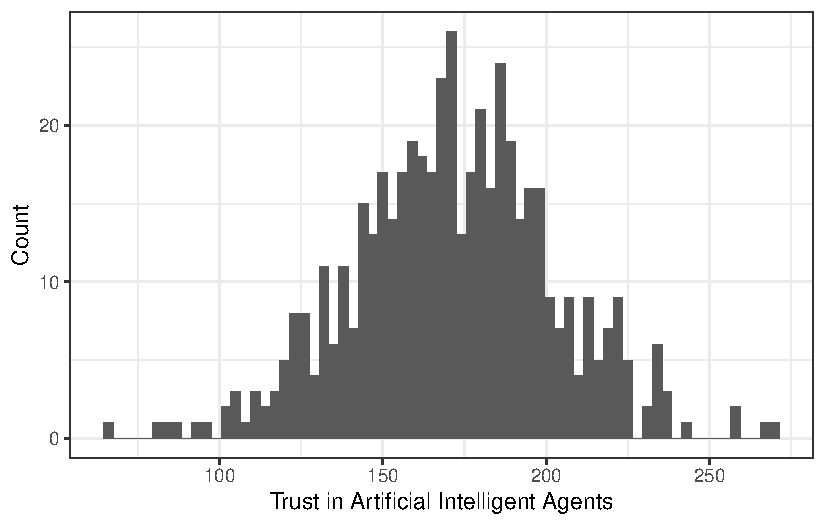
\includegraphics{andan-descriptives_files/figure-pdf/taia_score_vis-1.pdf}

Теперь нам понадобится определение квантиля распределения.

\textbf{Квантиль} --- это значение переменной, которое \emph{не
превышается} с определенной вероятностью (обозначим её \(p\)). Иначе
говоря, \emph{слева} от значения квантиля лежит \(p\%\) наблюдений.

Посмотрим на картинки.

\emph{Слева} относительно квантиля-0.05 (\(x_{0.05}\)) лежит 5\%
наблюдений:

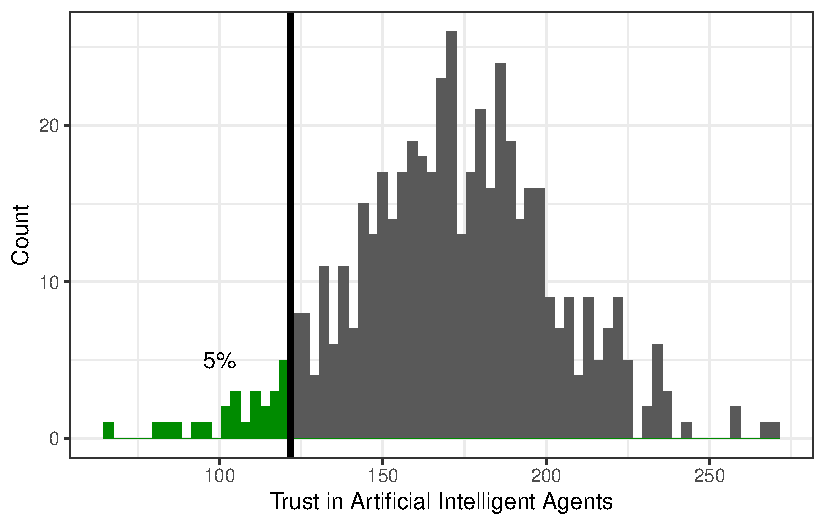
\includegraphics{andan-descriptives_files/figure-pdf/fifth_vis-1.pdf}

\emph{Слева} относительно квантиля-0.68 (\(x_{0.68}\)) лежит 68\%
наблюдений:

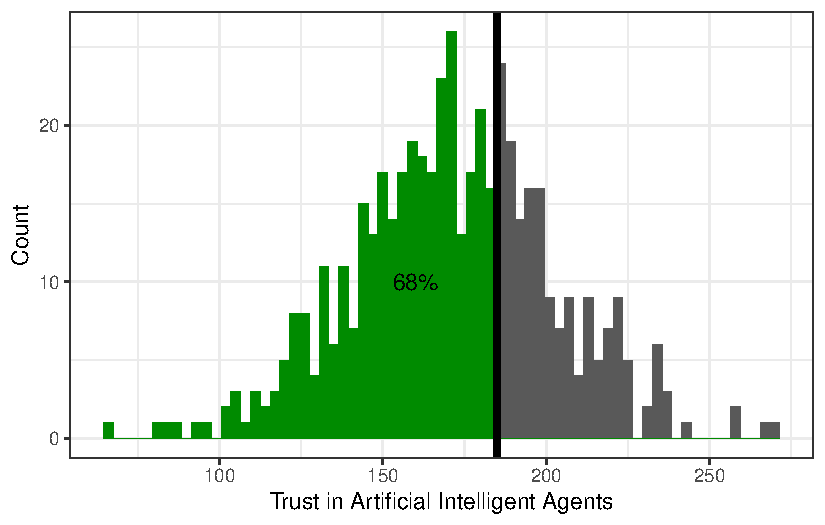
\includegraphics{andan-descriptives_files/figure-pdf/68_vis-1.pdf}

\emph{Слева} относительно квантиля-0.99 (\(x_{0.99}\)) лежит 99\%
наблюдений:

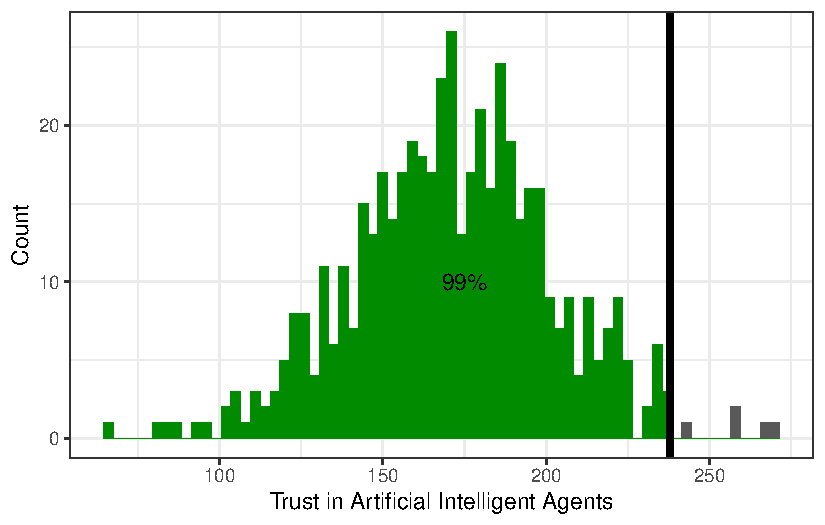
\includegraphics{andan-descriptives_files/figure-pdf/99_vis-1.pdf}

Итак, мы поняли, а также приняли и осознали, что такое квантиль. Неясно
только, как он нам поможет описать вариативность данных.

\subsection{Квартили}\label{quartiles}

Для этого нам пригодятся специально обученные квантили. Оказалось
достаточно удобно поделить все наблюдение на \emph{четыре} равные части
--- вот так:

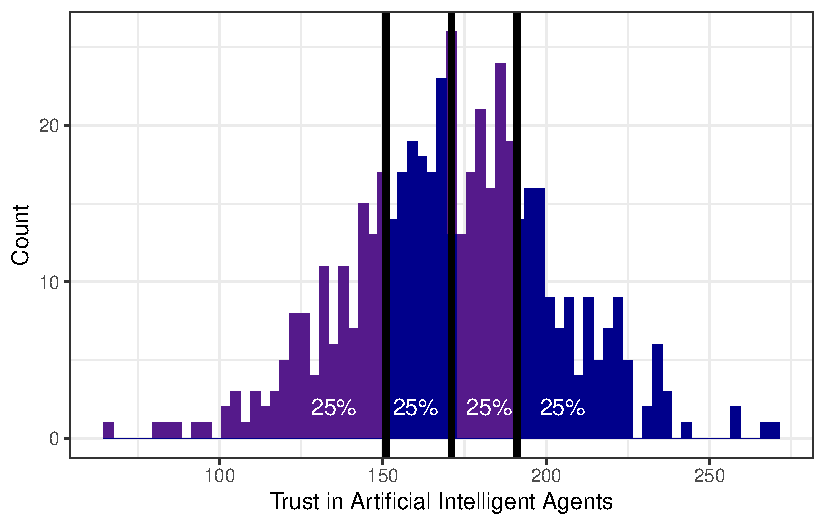
\includegraphics{andan-descriptives_files/figure-pdf/quartiles_vis-1.pdf}

Значения переменной, которые делят выборку на \emph{четыре} равные части
называются \textbf{квартили}. Получается, что

\begin{itemize}
\tightlist
\item
  слева от \textbf{первого (нижнего) квартиля} (\(Q_1\), \(x_{0.25}\))
  лежит 25\% наблюдений
\item
  слева от \textbf{второго (среднего) квартиля} (\(Q_2\), \(x_{0.50}\))
  лежит 50\% наблюдений

  \begin{itemize}
  \tightlist
  \item
    а значит и справа 50\% --- получается второй квартиль делит выборку
    пополам --- это \textbf{медиана}
  \end{itemize}
\item
  слева от \textbf{третьего (верхнего) квартиля} (\(Q_3\), \(x_{0.75}\))
  лежит 75\% наблюдений
\end{itemize}

Четвертый квартиль не используется, потому что это максимальное значение
--- слева от него лежит 100\% наблюдений.

Кстати, можно также отметить, что первый квартиль --- это медиана нижней
(меньшей) половины наблюдений, а третий --- медиана верней (большей)
половины наблюдений.

Вот такая вот прикольная история.

\subsection{Децили}\label{deciles}

К слову, делить выборку можно не только на четверти --- можно поделить,
скажем, на 10 частей и получить \textbf{децили}. Так, слева от
\emph{первого дециля} (\(x_{0.10}\)) лежит 10\% наблюдений, а слева от
\emph{третьего} (\(x_{0.30}\)) --- 30\%.

Децили встречаются редко (в основном в психометрике), но знать о них
полезно.

\subsection{Перцентили}\label{percentiles}

Гораздо чаще встречаются \textbf{перцентили} --- значения переменной,
которые делят выборку на 100 равных частей. Например, так устроен ваш
рейтинг. Только стоит помнить, что в рейтинге отсчет ведется от
максимального среднего балла, поэтому если у вас \emph{нулевой
перцентиль} (\(x_{0.00}\)) по программе, значит \emph{выше} вас в
рейтинге никого нет. А если ваш перцентиль, скажем, 36-ой
(\(x_{0.36}\)), то выше вас в рейтинге 36\% ваших однокурсников, то есть
вы все ещё в первой половине рейтинга, что очень неплохо!

\subsection{Интерквартильный размах}\label{iqr}

И --- о, ура! --- мы наконец-то добрались до того, ради чего тут
собрались! Зная первый и третий квартили распределения, можно рассчитать
\textbf{интерквартильный (межквартильный) размах (interquartile range,
IQR)}.

\[
\mathrm{IQR}(X) = Q_3(X) - Q_1(X)
\]

Интерквартильный размах --- это разница между третьим и первым квартилем
распределения. Эта величина описывает интервал значений признака, в
котором лежит 50\% наблюдений.

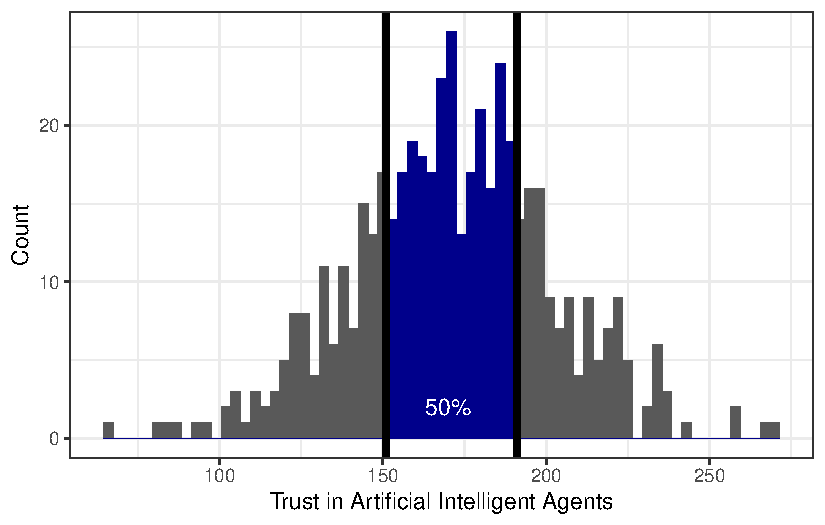
\includegraphics{andan-descriptives_files/figure-pdf/iqr_vis-1.pdf}

В данном случае он равен 40:

\begin{Shaded}
\begin{Highlighting}[]
\FunctionTok{IQR}\NormalTok{(taia}\SpecialCharTok{$}\NormalTok{DT)}
\end{Highlighting}
\end{Shaded}

\begin{verbatim}
[1] 40
\end{verbatim}

То есть 50\% наблюдений лежит в пределах 40 единиц шкалы.

\subsection{Визуализация квартилей. Боксплот}\label{boxplot}

Отображать квартили на гистограмме, во-первых, совершенно неудобно, а
во-вторых, не то чтобы график получается информативный. Для визуализации
квартилей придумали специальный тип графика --- \textbf{ящик с усами,
или боксплот (boxplot)}.

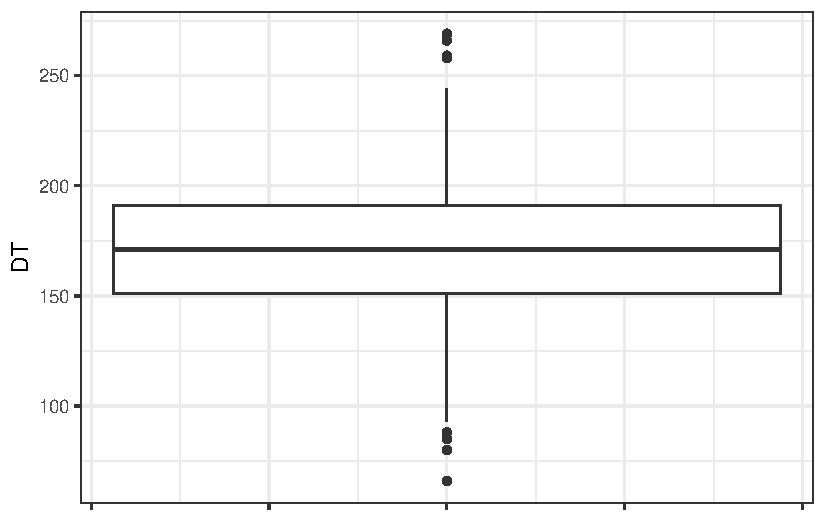
\includegraphics{andan-descriptives_files/figure-pdf/boxplot-1.pdf}

Прикольная ерунда. Научимся его читать.

Значения переменной идут по вертикальной оси (оси ординат). По
горизонтальной оси (оси абсцисс) здесь ничего не идет\footnote{Но если
  мы рисуем несколько боксплотов рядом, то на оси \texttt{x} будет
  категориальная переменная.}. Жирная линия по середине ящика ---
медиана (второй квартиль). Нижняя граница ящика --- первый квартиль,
верхняя --- третий. Получается, что границы ящика показывают нам
значения, в пределах которых лежит половина наблюдений.

Нижний ус --- первый квартиль минус полтора межквартильных размаха.
Верхний ус --- третий квартиль плюс полтора мехквартильных размаха.

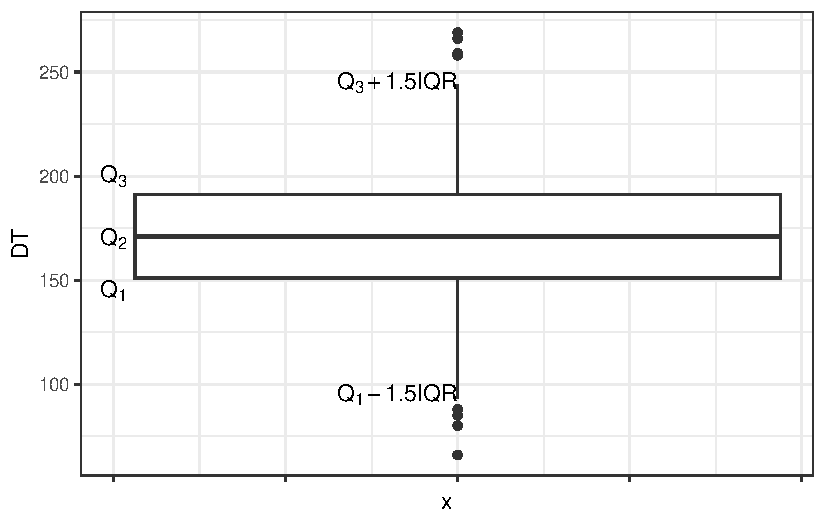
\includegraphics{andan-descriptives_files/figure-pdf/boxplot_annotated-1.pdf}

\emph{Замечание}

Ящик может быть асимметричным --- то есть верхняя его часть (расстояние
между медианой и третьим квартилем) и нижняя его часть (расстояние между
медианой и первым квартилем) могут быть разными. Это нам говорит об
асимметричности распределения. Усы также могут быть неравными, если один
из них упирается в максимум / минимум --- тоже по причине
асимметричности распределения.

Ну, допустим. А что тогда точки?

\subsubsection{Выбросы}\label{andan-descriptives-XX-iqr_outliers}

Вообще справедливо было бы задаться вопросом, а зачем нам вообще усы на
этом графике? И почему мы прибавляем полтора межквартильных размаха?

Это \emph{один из подходов} к определению нехарактерных значений ---
выбросов. При исследовании данных мы часто задаемся вопросом, если ли в
наших данных такие значения, которые сильно отличаются от распределения
той или иной переменной. Но как определить это самое «сильно»?

Вот один из подходов. Будем считать, что значения, которые укладываются
в интервал
\((Q_1 - 1.5 \times \mathrm{IQR}, \, Q_3 + 1.5 \times \mathrm{IQR})\),
нас устраивают. Все что попадает в этот интервал --- это «нормальные»,
типичные значения нашей переменной. Те же, которые будут находиться за
пределами этого интервала, мы назовем нетипичными, аномальными
значениями, или \textbf{выбросами}. Эти значения и будут отмечены
точками на графике boxplot.

Что с ними делать? Во-первых, содержательной анализировать. Выбросы
могут возникнуть по разным причинам. Может быть испытуемый отвлекся на
прилетевшего в окно голубя, и у нас в данных появилось время реакции 200
секунд. Такие выбросы мы можем исключить из данных. А возможно в нашу
выборку попали какие-то люди, которые, скажем, очень сильно или очень
слабо доверяют искусственному интеллекту (как в примере на рисунке). Эти
наблюдения необходимо дополнительно проанализировать --- возможно, это
представители специфических групп нашей генеральной совокупности
(например, программисты-разработчики или люди пенсионного возраста).
Анализ принесет нам дополнительную информацию, которую мы могли не
учесть при планировании исследования. Крч, думать надо. И собирать
побольше данных, чтобы можно было найти содержательную интерпретацию
происходящему.

\section{Сравнение мер
разброса}\label{andan-descriptives_variation_comparison}

Как и разные меры центральной тенденции, разные меры разброса по-своему
хороши. Более того, они дружат с мерами центральной тенденции. Так,
\emph{с медианой используется мехквартильных размах}, а \emph{со средним
арифметическим --- стандартное отклонение}.

Размах подходит для всего сразу. Его стоит рассчитать, чтобы составить
самое первое представление в разбросе, о границах измерения изучаемого
признака {[}на нашей выборке{]}.

Стоит также отметить, что все, что мы тут обсуждали, совершенно не
годиться для номинативных переменных. Однако у них тоже есть
вариативность. Согласитель, что выборка из Питера, Москвы, и Казани
более вариативна, чем выборка из Москвы. Аналогом меры разброса для
номинальной переменной можно назвать количество уникальных значений этой
переменной.

\section{Асимметрия}\label{andan-descriptives-skewness}

\section{Эксцесс}\label{andan-descriptives-kurtosis}

\section{Итоги}\label{andan-descriptives-final}

\bookmarksetup{startatroot}

\chapter{Сравнение средних}\label{andan-ttest}

\bookmarksetup{startatroot}

\chapter{Анализ категориальных данных}\label{andan-chisq}

\bookmarksetup{startatroot}

\chapter{Корреляционный анализ
\{\#andan-corr\}\}}\label{ux43aux43eux440ux440ux435ux43bux44fux446ux438ux43eux43dux43dux44bux439-ux430ux43dux430ux43bux438ux437-andan-corr}

До этого момента мы рассматривали только отдельные переменные и их
характерики, однако в практике мы редко работаем только с одной
переменной. Как правило, у нас есть многомерное пространство признаков,
и нас интересуют взаимосвязи между ними.

\section{Ковариация}\label{andan-corr-cov}

Мы хотим описать имеющиеся взаимосвязи как можно проще и опираясь на то,
что у нас уже есть. Мы говорили, что дисперсия, или вариация, заключает
в себе информацию об изменчивости признака. Если мы хотим исследовать
взаимосвязь между признаками, то логично будет посмотреть, как
изменяется один из признаков при изменении другого --- иначе говоря,
рассчитать \emph{совместную изменчивость признаков}, или
\textbf{ко-вариацию (covariance)}.

Как мы её будем считать? Подумаем графически. Расположим две переменные
на осях и сопоставим каждому имеющемуся наблюдению точку на плоскости.

КАРТИНКА

Отметим средние значения по обеим переменным.

КАРТИНКА

Заметим, что если наши наблюдения по переменной \(x_1\) отклоняются в
большую сторону, то они отклоняются в большую сторону и по переменной
\(x_2\). Аналогично, если они будут отклоняться в меньшую сторону по
\(x_1\), то в меньшую же сторону они будут отклоняться и по \(x_2\).

КАРТИНКА

Получается, мы можем на основании согласованности отклонений уже
заключить о направлении связи. \emph{Произведение отклонений по обеим
величинам будет положительно, если отклонения сонаправленны}. Запишем
это математически.

\[
(\bar x_1 - x_{i1}) (\bar x_2 - x_{i2}) > 0 \Leftarrow \big( (\bar x_1 - x_{i1}) > 0 \wedge (\bar x_2 - x_{i2}) > 0 \big) \vee \big( (\bar x_1 - x_{i1}) < 0 \wedge (\bar x_2 - x_{i2}) < 0 \big)
\]

Соответственно, если отклонения будут направлены в разные стороны, из
произведение будет отрицательным. Ну, осталось только понять, как
совместные отклонения организованы в среднем --- это и будет ковариацией
двух величин:

\[
\mathrm{cov}(X_1, X_2) = \frac{1}{n-1} \sum_{i=1}^n (\bar x_1 - x_{i1}) (\bar x_2 - x_{i2})
\]

Что такое ковариация величины самой с собой
(\(\mathrm{cov}(X_1, X_1)\))?

Попробуйте получить ответ через вывод формулы.

Важно отметить, что ковариация улавливается только \emph{линейную
составляющую} взаимосвязи между признаками, поэтому если
\(\mathrm{cov}(X_1,X_2) = 0\), то мы можем сказать, что между
переменными нет \emph{линейной} взаимосвязи, однако это не значит, что
между этими переменными нет никакой другой зависимости.

КАРТИНКА

У ковариации есть два важных недостатка:

\begin{itemize}
\tightlist
\item
  это размерная величина, поэтому её значение зависит от единиц
  измерения признаков,
\item
  она зависит от дисперсий признаков, поэтому по её значению можно
  определить только направление связи (прямая или обратная), однако
  ничего нельзая сказать о силе связи.
\end{itemize}

Поэтому нам нужно как-то модицифировать эту статистику, чтобы мы могли
больше вытащить из её значения.

\section{Корреляция}\label{andan-corr-cor}

Раз ковариация зависит от дисперсии, то можно сделать некоторые
математические преобразования, чтобы привести эмпирические распределения
к какому-то одному виду --- сделать так, чтобы они имели одинакое
математическое ожидание (среднее) и одинаковую дисперсию. С этой задачей
прекрасно справляется \hyperref[standartization]{стандартизация}.
Напоминаю формулу:

\[
x_i^* = \frac{x_i - \bar x}{s}
\]

После такого преобразования математическое ожидание нашего распределения
будет равно нуля, а стандартное отклонение --- единице. Это избавит нас
от влияния дисперсии на значение ковариации. Ковариация двух стандартно
нормально распределенных величин называется \textbf{корреляцией
(correlation)}.

\[
\mathrm{cov}(X_1^*, X_2^*) = \frac{1}{n-1} \sum_{i=1}^n x_{i1}^* x_{i2}^* = \mathrm{corr}(X_1, X_2),
\] где \(X_1^*\) и \(X_2^*\) --- стандартизированные величины \(X_1\) и
\(X_2\) соответственно.

Корреляцию можно выразить через ковариацию:

\[
\mathrm{corr}(X_1, X_2) = \frac{1}{n-1} \sum_{i=1}^n \Big( \frac{\bar x_1 - x_{i1}}{s_1} \Big) \Big( \frac{\bar x_2 - x_{i2}}{s_2} \Big) = 
\frac{1}{s_1 s_2} \Big( \frac{1}{n-1} \sum_{i=1}^n (\bar x_1 - x_{i1})(\bar x_2 - x_{i2}) \Big) = \frac{\mathrm{cov}(X_1, X_2)}{s_1 s_2}
\]

Если внимательно всмотреться в формуле, то можно обнаружить, что
корреляция это не что иное, как стандартизированное значение ковариации.

Коэффициент корреляции имеет четкие пределы изменения: \([-1; \,1]\).
Крайнее левое значение говорит о том, что присутствует полная обратная
линейная взаимосвязь, крайнее правое --- что присутствует полная прямая
линейная взаимосвязь. Как и ковариация, корреляция ловит \emph{только
линейную составляющую} связи, поэтому нулевое значение корреляци
показывает, что между переменными отсутствует \emph{линейная
взаимосвязь}. Это всё еще не значит, что связи нет вовсе.

\subsection{Тестирование статистической значимости коэффициента
корреляции}\label{andan-corr-test}

Оценку коэффициента корреляции мы получаем методом моментов, заменяя
истинный момент \(\rho_{ij}\) выборочным \(r_{ij}\):

\[
\hat \rho_{ij} = \overline{\big( (X_{ki} - \bar X_i) (X_{kj} - \bar X_j) \big)} = r_{ij}
\]

Если в генеральной совокупности связь между признаками отсутствует, то
есть \(\rho_{ij} = 0\), будет ли равен нулю \(r_{ij}\)? Можно с
уверенностью сказать, что не будет, так как выборочный коэффициент
корреляции --- случайная величина. А мы помним, что вероятность принятия
случайной величиной своего конкретного значения равна нулю.

Тогда необходимо протестировать статистическую гипотезу:

\[
H_0: \rho_{ij} = 0 \; \text{(линейной связи нет)} \\
H_1: \rho_{ij} \neq 0 \text{(наиболее частый вариант альтернативы)}
\]

Для проверки нулевой гипотезы используется следующая статистика:

\[
t = \frac{r_{ij}}{\sqrt{\frac{1 - r^2_{ij}}{n-2}}} \overset{H_0}{\thicksim} t(\nu = n-2)
\]

Вывод о статистической значимости коэффициента корреляции делается
согласно \hyperref[statestim]{алгоритму тестировния статистических
гипотез}.

\subsection{Доверительный интервал для коэффициента
корреляции}\label{ux434ux43eux432ux435ux440ux438ux442ux435ux43bux44cux43dux44bux439-ux438ux43dux442ux435ux440ux432ux430ux43b-ux434ux43bux44f-ux43aux43eux44dux444ux444ux438ux446ux438ux435ux43dux442ux430-ux43aux43eux440ux440ux435ux43bux44fux446ux438ux438}

С построением интервальной оценки коэффциента корреляции возникают
некоторые сложности. Наша задача состоит в том, чтобы определить в каких
границах будет лежать значение истинного коэффициента корреляции с
заданной вероятностью:

\[
\mathrm{P} (\rho_{ij,\min} < \rho_{ij} < \rho_{ij,\max}) = \gamma
\]

Нам необходимо найти статистику, закон распределения корой известен,
однако ранее упомянутся статистика не подходит, так как она имеет
распределение Стьюдента, когда верна нулевая гипотеза об отсутствии
связи. Если же мы строим интервальную оценку, нас интересует случай
наличия связи.

Такую статистику искали долго, и её удалось найти, когда ввели
определённое преобразование выборочного критерия корреяции ---
\emph{z-преобразования Фишера}:

\[
z(r_{ij}) = \frac{1}{2} \ln \frac{1 + r_{ij}}{1 - r_{ij}} \thicksim \mathrm{N}(\bar z_{ij}, \tfrac{1}{n-3}),
\] где \(n\) --- объём выборки, а \(\bar z_{ij}\) получается расчётом по
указанной формуле после подставления точечной оценки коэффициента
корреляции.

Тогда интервальная оценка для величины \(z_{ij, \mathrm{true}}\)
приобретает такой вид:

\[
\mathrm{P} \Big( \bar z_{ij} - t_\gamma \sqrt{\tfrac{1}{n-3}} < z_{ij, \mathrm{true}} < \bar z_{ij} + t_\gamma \sqrt{\tfrac{1}{n-3}}  \Big) = \gamma = \Phi(t_\gamma)
\]

Далее путём обратного преобразования получаются значения границ
интервала \((\rho_{ij,\min}, \; \rho_{ij,\max})\).

\section{Коэффициенты корреляции для разных
шкал}\label{andan-corr-scales}

Дла разных шкал разработаны разные коэффициенты корреляции. Оценки
коэффициентов будут рассчитываться по-разному, но логика тестирования
статистических гипотез остаётся одинаковой.

\begin{longtable}[]{@{}
  >{\centering\arraybackslash}p{(\columnwidth - 4\tabcolsep) * \real{0.3333}}
  >{\centering\arraybackslash}p{(\columnwidth - 4\tabcolsep) * \real{0.3333}}
  >{\centering\arraybackslash}p{(\columnwidth - 4\tabcolsep) * \real{0.3333}}@{}}
\toprule\noalign{}
\begin{minipage}[b]{\linewidth}\centering
Переменная \(X\)
\end{minipage} & \begin{minipage}[b]{\linewidth}\centering
Переменная \(Y\)
\end{minipage} & \begin{minipage}[b]{\linewidth}\centering
Мера связи
\end{minipage} \\
\midrule\noalign{}
\endhead
\bottomrule\noalign{}
\endlastfoot
Интервальная или отношений & Интервальная или отношений & Коэффициент
Пирсона \\
Ранговая, интервальная или отношений & Ранговая, интервальная или
отношений & Коэффициент Спирмена \\
Ранговая & Ранговая & Коэффициент Кенделла \\
\end{longtable}

В функциях \texttt{cor()} и \texttt{cor.test()} требуемый коэффициент
задаётся черед аргумент \texttt{method}:

\section{Частный и множественный коэффициент
корреляции}\label{ux447ux430ux441ux442ux43dux44bux439-ux438-ux43cux43dux43eux436ux435ux441ux442ux432ux435ux43dux43dux44bux439-ux43aux43eux44dux444ux444ux438ux446ux438ux435ux43dux442-ux43aux43eux440ux440ux435ux43bux44fux446ux438ux438}

Если у нас два признака, то с ними всё достаточно понятно. А если
признаком много? Тогда у нас могут быть сложные взаимосвязи, и возможен
такой случай, что некоторый признак оказывает связан как с одним, так и
с другим из интересующих нас. Таким образом, мы можем наблюдать
\emph{ложную корреляцию}. Чтобы избавиться от влияния сторонних
признаков, используюся частные коэффициенты корреляции.

Функция \texttt{cor()} может возвращать не только оценку одного
коэффициента корреляции, но и \textbf{корреляционную матрицу},
отобрадающую связи всех признаков со всеми. Например, продолжим работать
со шкалой морального возмущения и изучим взаимосвязи внутри неё:

В корреляционной матрице на главной диагонали стоят единицы, отражающай
связь переменной в самой собой --- разумеется, она будет абсолютно
линейная.

А как посчитать \emph{ковариационную} матрицу?

В общем виде корреляционная матрица имеет следующий вид:

\[
R = 
\begin{pmatrix}
1 & r_{12} & \dots & r_{1p} \\
r_{12} & 1 & \dots & r_{2p} \\
\vdots & \vdots & \ddots & \vdots \\
r_{p1} & r_{p2} & \dots & 1
\end{pmatrix}
\]

Матрица, как можно заметить, симметрична относительно главной диагонали,
так как \(r_{ij} = r_{ji}\).

Её можно визуализироать, например, так:

Но можно и усовершенствовать визуализацию, отобразив сами значения:

На основе этой матрицы мы можем протестировать статистическую значимость
каждого из коэффициентов (не забыв про поправки на множественные
сравнения!):

Чтобы перенести их на график, нам нужно получить матрицу из p-значений:

Ну, у нас ничего не поменялось, так как коэффициенты все оказались
значимы. Эх\ldots{}

Но вот для примера на одно из встроенных датасетов:

Итак, возвращается к частному коэффициенту корреляции. Он определяется
так:

\[
r_{ij, J(i,j)} = - \frac{A_{ij}}{\sqrt{A_{ii} A_{jj}}},
\]

где \(A\) --- алгебраическое дополнение.

В общем виде это осознать сложно, поэтому давайте на примере трёх
признаков.

\[
R =
\begin{pmatrix}
1 & r_{12} & r_{13} \\
r_{21} & 1 & r_{23} \\
r_{31} & r_{32} & 1
\end{pmatrix}
\]

\[
r_{12,3} = \frac{r_{12} - r_{13} \cdot r_{23}}{\sqrt{(1 - r^2_{23})(1-r^2{13})}}
\]

\[
H_0: \rho_{12,3} = 0 \\
H_1: \rho_{12,3} \neq 0 \\
t = \frac{r_{12,3} \sqrt{n-3}}{\sqrt{1 - r^2_{12,3}}} \overset{H_0}{\thicksim} t(\nu = n-3)
\]

Но слава богу, что в R это все делается в одну строку:

Хорошо, а если нас интересует связь одного признака с несколькими сразу?
Тогда нам нужен множественный коэффициент корреляции. Он также
вычисляется на основе корреляционной матрицы и определяется следующим
образом. Пусть нас интересует связь первого признака со всеми
остальными:

\[
R_1 = \sqrt{1 - \frac{\det R}{A_{11}}}
\]

Квадрат множественонго коэффициента корреляции называется
\emph{коэффициентом детерминации}\footnote{Вы точно видели это
  словосочетание, когда сталкивались с линейной регресией.}. Он
показывает, во-первых, степень тесноты связи данного признака со всеми
остальными, но, кроме того, ещё и долю дисперсии данного признака,
определяемую вариацией все остальных признаков, включенных в данную
корреляционную модель.

Мы подробнее его изучим в следуюшей теме, а также увидим, где нам его
найти, чтобы не считать руками.

\section{Другие
корреляции}\label{ux434ux440ux443ux433ux438ux435-ux43aux43eux440ux440ux435ux43bux44fux446ux438ux438}

Можно коррелировать не только количественные и ранговые шкалы между
собой, но и качественные тоже:

\begin{longtable}[]{@{}ccc@{}}
\toprule\noalign{}
Переменная \(X\) & Переменная \(Y\) & Мера связи \\
\midrule\noalign{}
\endhead
\bottomrule\noalign{}
\endlastfoot
Дихотомическая & Дихотомическая & \(\phi\)-коэффициент \\
Дихотомическая & Ранговая & Рангово-бисериальный коэффициент \\
Дихотомическая & Интервальная или отношений & Бисериальный
коэффициент \\
\end{longtable}

\subsection{\texorpdfstring{\(\phi\)-коэффициент}{\textbackslash phi-коэффициент}}\label{phi-ux43aux43eux44dux444ux444ux438ux446ux438ux435ux43dux442}

Этот коэффициент позволяет рассчитать корреляцию между двумы
дихотомическими шкалами. Он основан на расчёте статистики \(\chi^2\).

По двум дихотомическим переменным можно построить таблицу сопряженности.
Разберемся на
\href{https://raw.githubusercontent.com/angelgardt/hseuxlab-wlm2021/master/book/wlm2021-book/data/cats_n_dogs.csv}{котиках
и пёсиках}:

По данной таблице можно рассчитать \textbf{критерий согласия Пирсона
(\(\chi^2\))}:

Сам хи-квадрат тестирует гипотезу о том, что между двумя категориальными
переменными нет связи. Он это делает путём сравнения теоретической и
эмпирической таблицы частот.

Эмпирическую таблицу частот мы получаем по результатам наблюдений (то,
что мы делаем с помощью функции \texttt{table()}):

\begin{longtable}[]{@{}ccc@{}}
\toprule\noalign{}
& \(X_1\) & \(X_2\) \\
\midrule\noalign{}
\endhead
\bottomrule\noalign{}
\endlastfoot
\(Y_1\) & \(p_{X_1,Y_1} = a\) & \(p_{X_2,Y_1} = b\) \\
\(Y_2\) & \(p_{X_1,Y_2} = c\) & \(p_{X_2,Y_2} = d\) \\
\end{longtable}

Далее вычисляются теоретические частоты:

\begin{longtable}[]{@{}
  >{\centering\arraybackslash}p{(\columnwidth - 4\tabcolsep) * \real{0.3333}}
  >{\centering\arraybackslash}p{(\columnwidth - 4\tabcolsep) * \real{0.3333}}
  >{\centering\arraybackslash}p{(\columnwidth - 4\tabcolsep) * \real{0.3333}}@{}}
\toprule\noalign{}
\begin{minipage}[b]{\linewidth}\centering
\end{minipage} & \begin{minipage}[b]{\linewidth}\centering
\(X_1^*\)
\end{minipage} & \begin{minipage}[b]{\linewidth}\centering
\(X_2^*\)
\end{minipage} \\
\midrule\noalign{}
\endhead
\bottomrule\noalign{}
\endlastfoot
\(Y_1^*\) & \(\frac{(a+b) \times (a+c)}{N}\) &
\(\frac{(b+a) \times (b+d)}{N}\) \\
\(Y_2^*\) & \(\frac{(c+d) \times (a+c)}{N}\) &
\(\frac{(d+c) \times (b + d)}{N}\) \\
\end{longtable}

где \(N = a + b + c + d\).

Затем считаются расхождения частот, которые суммируются и получается
статистика \(\chi^2\):

\[
\chi^2 = \sum_{i,j} \frac{p_{X_i,Y_j} - p_{X_i^*,Y_j^*}}{p_{X_i^*,Y_j^*}}
\]

Статистика подчиняется распределению \(\chi^2\), и чем больше значение
этой статистики, тем сильнее связаны признаки. В нашем случае мы
получили значение 0, что говорит о абсолютном отсутствии связи между
видом животного и его размером.

Но по значению \(\chi^2\) сложно что-то сказать о силе связи, поэтому
его нормируют следующим образом, чтобы получить значения от 0 до 1,
которые можно интерпретироват аналогично коэффициенту корреляции:

\[
\phi = \sqrt{\frac{\chi^2}{N}}
\]

Так как в нашем случае значение \(\chi^2\) было 0, то и коэффициент
\(\phi\) мы получили 0.

\subsection{Бисериальный коэффициент
корреляции}\label{ux431ux438ux441ux435ux440ux438ux430ux43bux44cux43dux44bux439-ux43aux43eux44dux444ux444ux438ux446ux438ux435ux43dux442-ux43aux43eux440ux440ux435ux43bux44fux446ux438ux438}

Этот коэффициент используется для вычисления корреляции между
количественной (\(y\)) и категориальной (\(x\)) шкалой и рассчитывается
следующим образом:

\[
r = \frac{\bar x_1 - \bar x_2}{s_y} \sqrt{\frac{n_1 n_2}{N(N-1)}},
\] где \(\bar x_1\) --- среднее по элементам переменной \(y\) из группы
\(x_1\), \(\bar x_2\) --- среднее по элементам \(y\) из группы \(x_2\),
\(s_y\) --- стандартное отклонение по переменной \(y\), \(n_1\) ---
число элементов в группе \(x_1\), \(n_2\) --- число элементов в группе
\(x_2\), \(N\) --- общее число элементов.

Важно отметить, что несмотря на то, что значение коэффициента может быть
как положительным, так и отрицательным, это \emph{не влияет на
интерпретацию}. Это одно из исключений из общего правила.

В R его можно вычислить так:

\subsection{Рангово-бисериальный коэффициент
корреляции}\label{ux440ux430ux43dux433ux43eux432ux43e-ux431ux438ux441ux435ux440ux438ux430ux43bux44cux43dux44bux439-ux43aux43eux44dux444ux444ux438ux446ux438ux435ux43dux442-ux43aux43eux440ux440ux435ux43bux44fux446ux438ux438}

Если у нас не количественная, а ранговая шкала, то применяется
рангово-бисериальный коэффициент:

\[
r = \frac{2(\bar x_1 - \bar x_2)}{N},
\] где \(\bar x_1\) --- средний ранг в группе \(x_1\), \(\bar x_2\) ---
средний ранг в группе \(x_2\), \(N\) --- общее количество наблюдений.

\section{Преобразование Фишера}\label{andan-cor-fisher-transform}

\[
z_i = \frac{1}{2} \ln \frac{1 + r_i}{1 - r_i} = \artanh (r_i)
\]

\[
r_P = \dfrac{e^{2z_P} - 1}{e^{2z_P} + 1} = \tanh(z_P)
\]

\bookmarksetup{startatroot}

\chapter{Непараметрические методы анализа данных}\label{andan-nonparam}

\bookmarksetup{startatroot}

\chapter{Общие линейные модели. Простая линейная
регрессия}\label{andan-simplelinear}

\section{Вычисление коэффициентов линейной
регрессии}\label{ux432ux44bux447ux438ux441ux43bux435ux43dux438ux435-ux43aux43eux44dux444ux444ux438ux446ux438ux435ux43dux442ux43eux432-ux43bux438ux43dux435ux439ux43dux43eux439-ux440ux435ux433ux440ux435ux441ux441ux438ux438}

\subsection{Матричное вычисление
коэффициентов}\label{ux43cux430ux442ux440ux438ux447ux43dux43eux435-ux432ux44bux447ux438ux441ux43bux435ux43dux438ux435-ux43aux43eux44dux444ux444ux438ux446ux438ux435ux43dux442ux43eux432}

\subsection{Аналитическое вычисление
коэффициентов}\label{ux430ux43dux430ux43bux438ux442ux438ux447ux435ux441ux43aux43eux435-ux432ux44bux447ux438ux441ux43bux435ux43dux438ux435-ux43aux43eux44dux444ux444ux438ux446ux438ux435ux43dux442ux43eux432}

\[
f(b_0, b_1) = \sum (y_i - \hat y_i)^2 = \sum (y_i - b_0 - b_1x_i)^2 \rightarrow \min_{b_0, b_1}
\]

\[
f(b_0, b_1) = \sum (y_i - b_0 - b_1x_i) (y_i - b_0 - b_1x_i)
\]

\[
f(b_0, b_1) = 
\sum (y_i^2 - b_0 y_i - b_1 x_i y_i - b_0 y_i - b_1 x_i y_i + b_0 b_1 x_i + b_1^2 x_i^2 + b_0^2 + b_0 b_1 x_i)
\]

\[
f(b_0, b_1) = 
\sum(y_i^2 - 2 b_1 x_i y_i - 2 y_i b_0 + x_i^2 b_1^2 + b_0^2 + 2 x_i b_1 b_0)
\]

\[
\frac{f(b_0, b_1)}{\partial b_0} = \sum (-2y_i + 2b_0 + 2x_ib_1) = 
-2 \sum \big( y_i - (b_0 + b_1 x_i) \big)
\]

\[
\frac{f(b_0, b_1)}{\partial b_1} = \sum (-2 x_i y_i + 2 x_i^2 b_1 + 2 x_i b_0) = -2 \sum \big( y_i - (b_0 + b_1 x_i) \big) x_i
\]

\[
\cases {
-2 \sum \big( y_i - (b_0 + b_1 x_i) \big) = 0 \\
-2 \sum \big( y_i - (b_0 + b_1 x_i) \big) x_i = 0
}
\]

\[
\cases{
\sum \big( y_i - (b_0 + b_1 x_i) \big) = 0 \\
\sum \big( y_i - (b_0 + b_1 x_i) \big) x_i = 0
}
\]

\[
\cases{
\sum y_i - \sum b_0 + \sum b_1 x_i = 0 \\
\sum y_i x_i - \sum b_0 x_i + \sum b_1 x^2_i = 0
}
\]

\[
\cases{
\sum b_0 + \sum b_1 x_i = \sum y_i \\
\sum b_0 x_i + \sum b_1 x_i^2 = \sum y_i x_i
}
\]

\[
\cases{
b1 \sum x_i + n b_0 = \sum y_i \\
b1 \sum x^2_i + b_0 \sum x_i = \sum y_i x_i
}
\]

\[
b_0 = \frac{\sum y_i}{n} - b_1 \frac{\sum x_i}{n} = \bar y - b_1 \bar x
\]

\[
b1 \sum x_i^2 + (\bar y - b_1 \bar x) \sum x_i = \sum x_i y_i
\]

\[
\underline{b_1 \sum x_i^2} + \bar y \sum x_i - \underline{b_1 \bar x \sum x_i} = \sum x_i y_i
\]

\[
b_1 \Big( \sum x_i^2 - \bar x \sum x_i \Big) = 
\sum x_i y_i - \bar y \sum x_i
\]

\[
b_1 = \frac{\sum x_i y_i - \bar y \sum x_i}{\sum x_i^2 - \bar x \sum x_i} = 
\frac{(\sum x_i y_i - \bar y \sum x_i) \times n}{(\sum x_i^2 - \bar x \sum x_i) \times n}
\]

\[
b_1 = \frac{\overline{xy} - \bar x \bar y}{\overline{x^2} - \bar x^2} = 
\frac{\overline{xy} - \bar x \bar y}{\sigma_X^2}
\]

\subsection{Угловой коэффициент и коэффициент
корреляции}\label{ux443ux433ux43bux43eux432ux43eux439-ux43aux43eux44dux444ux444ux438ux446ux438ux435ux43dux442-ux438-ux43aux43eux44dux444ux444ux438ux446ux438ux435ux43dux442-ux43aux43eux440ux440ux435ux43bux44fux446ux438ux438}

\[
b_1 = r_{X,Y} \times \frac{s_Y}{s_X}
\]

\[
r_{X,Y} = \frac{\sum (x_i - \bar x)(y_i - \bar y)}{\sqrt{\sum(x_i - \bar x)^2 \sum(y_i - \bar y)^2}}
\]

\[
b_1 = \frac{\sum (x_i - \bar x)(y_i - \bar y)}{\sqrt{\sum(x_i - \bar x)^2 \sum(y_i - \bar y)^2}}
\times
\frac{s_Y}{s_X}
\]

\[
b_1 = \frac{\sum (x_i - \bar x)(y_i - \bar y)}{\sqrt{\sum(x_i - \bar x)^2 \sum(y_i - \bar y)^2}}
\times
\frac{\sqrt{\sum (y_i - \bar y)^2 / (n-1)}}{\sqrt{\sum (x_i - \bar x)^2 / (n-1)}}
\]

Сократим дробь:

\[
\frac{\sqrt{(y_i - \bar y)^2 / (n-1)}}{\sqrt{(x_i - \bar x)^2 / (n-1)}} = 
\frac{\sqrt{(y_i - \bar y)^2} \times \sqrt{(n-1)}}{\sqrt{(x_i - \bar x)^2} \times \sqrt{(n-1)}} = \frac{\sqrt{(y_i - \bar y)^2}}{\sqrt{(x_i - \bar x)^2}}
\]

\[
b_1 = \frac{\sum (x_i - \bar x)(y_i - \bar y)}{\sqrt{\sum(x_i - \bar x)^2} \times \color{green}{\sqrt{\sum(y_i - \bar y)^2}}}
\times
\frac{\color{green}{\sqrt{\sum(y_i - \bar y)^2}}}{\sqrt{\sum(x_i - \bar x)^2}}
\]

\[
b_1 = \frac{\sum (x_i - \bar x)(y_i - \bar y)}{\sum(x_i - \bar x)^2}
\]

Сумма отклонений от среднего \href{}{равна нулю}:

\[
\sum(x_i - \bar x) = \sum (y_i - \bar y) = 0
\]

Разложим числитель:

\[
\sum (x_i - \bar x) (y_i - \bar y) = 
\sum x_i (y_i - \bar y) - \sum \bar x (y_i - \bar y) = 
\sum x_i (y_i - \bar y)
\]

\[
b_1 = \frac{\sum x_i (y_i - \bar y)}{\sum (x_i - \bar x)^2} = 
\frac{\Big( \sum x_i (y_i - \bar y) \Big) \times n}{\Big( \sum (x_i - \bar x)^2 \Big) \times n} = \frac{\overline{xy} - \bar x \bar y}{\sigma_X^2}
\]

\subsection{TSS = ESS + RSS?}\label{tss-ess-rss}

\[
\mathrm{TSS} = 
\sum (y_i - \bar y)^2 = 
\sum (y_i - \hat y + \hat y - \bar y)^2 = 
\sum \big( (y_i - \hat y_i) + (\hat y_i - \bar y) \big)^2 = 
\]

\[
= \sum (y_i - \hat y_i) = \sum (\hat y_i - \bar y) + 2 \sum (y_i - \hat y_i)(\hat y_i - \bar y) = 
\]

\[
= \mathrm{RSS} + \mathrm{ESS} + 2 \sum (y_i - \hat y_i)(\hat y_i - \bar y)
\]

Окей, осталось доказать, что
\(2 \sum (y_i - \hat y_i)(\hat y_i - \bar y) = 0\), и все будет найс.

Так как \(b_0 = \bar y - b_1 x\).

\[
\sum (y_i - \hat y_i)(\hat y_i - \bar y) = \sum (y_i - b_0 - b_1 x_i) (b_0 + b_1 x_i - \bar y) =
\]

\[
= \sum (y_i - \bar y + b_1 \bar x - b_1x_i) (\bar y - b_1 \bar x + b_1 x_i - \bar y) =
\]

\[
= \sum \big( (y_i - \bar y) - b_1(x_i - \bar x) \big) \times b_1 (x_i - \bar x) = 
\sum \big( b_1 (x_i - \bar x) (y_i - \bar y) - b_1^2 (x_i - \bar x)^2 \big) = 
\]

\[
= b_1 \sum (x_i - \bar x) (y_i - \bar y) - b_1^2 \sum (x_i - \bar x)
\]

Так как
\(b_1 = \frac{\sum(x_i - \bar x)(y_i - \bar y)}{\sum (x_i - \bar x)^2}\),
получается, что:

\[
\frac{\Big( \sum (x_i - \bar x) (y_i - \bar y) \Big)^2}{\sum (x_i - \bar x)^2} - \frac{\Big( \sum (x_i - \bar x) (y_i - \bar y) \Big)^2 \times \sum (x_i - \bar x)^2}{\Big( \sum (x_i - \bar x)^2\Big)^2} = 
\]

\[
= \frac{\Big( \sum (x_i - \bar x) (y_i - \bar y) \Big)^2}{\sum (x_i - \bar x)^2} - \frac{\Big( \sum (x_i - \bar x) (y_i - \bar y) \Big)^2}{\sum (x_i - \bar x)^2} = 0
\]

\bookmarksetup{startatroot}

\chapter{Множественная линейная регрессия}\label{andan-multiplelinear}

\bookmarksetup{startatroot}

\chapter{Полиномиальная регрессия}\label{andan-polynomial}

\bookmarksetup{startatroot}

\chapter{Support Vector Regression}\label{andan-svr}

\bookmarksetup{startatroot}

\chapter{Регуляризованная регрессия}\label{andan-regreg}

\bookmarksetup{startatroot}

\chapter{Дисперсионный анализ}\label{andan-anova}

\bookmarksetup{startatroot}

\chapter{Ковариационный анализ}\label{andan-ancova}

\bookmarksetup{startatroot}

\chapter{Многомерный дисперсионный анализ}\label{andan-manova}

\bookmarksetup{startatroot}

\chapter{Деревья решений. Регрессия}\label{andan-treesreg}

\bookmarksetup{startatroot}

\chapter{Случайный лес. Регрессия}\label{andan-randforestreg}

\bookmarksetup{startatroot}

\chapter{Определение вида распределения
переменной}\label{andan-distributions}

\bookmarksetup{startatroot}

\chapter{Обобщенные линейные модели. Логистическая
регрессия}\label{andan-logreg}

\section{Линеаризация логистической кривой посредством
logit-преобразования}\label{ux43bux438ux43dux435ux430ux440ux438ux437ux430ux446ux438ux44f-ux43bux43eux433ux438ux441ux442ux438ux447ux435ux441ux43aux43eux439-ux43aux440ux438ux432ux43eux439-ux43fux43eux441ux440ux435ux434ux441ux442ux432ux43eux43c-logit-ux43fux440ux435ux43eux431ux440ux430ux437ux43eux432ux430ux43dux438ux44f}

\[
p = \frac{e^{\beta_0 + \beta_1 x}}{1 + e^{\beta_0 + \beta_1 x}}
\]

Произведем замену:

\[
\beta_0 + \beta_1 x = t
\]

\[
\mathrm{logit}(p) = \ln \Big( \frac{p}{1-p} \Big)
\]

Если logit-преобразование действительно линеризует логистическую кривую,
что должно выполняться равенство:

\[
\mathrm{logit}(p) = t \Rightarrow \ln \Big( \frac{p}{1-p} \Big) = t
\]

Докажем это.

\[
\ln \Big( \frac{p}{1-p} \Big) = 
\ln \Bigg( \frac{\frac{e^t}{1 + e^t}}{1 - \frac{e^t}{1 + e^t}} \Bigg) =
\ln \Big( \frac{e^t}{1 + e^t} \Big) - \ln \Big(1 - \frac{e^t}{1 + e^t} \Big) = 
\]

\[
= \ln \Big( \frac{e^t}{1 + e^t} \Big) - \ln \Big(\frac{1 + e^t - e^t}{1 + e^t} \Big) = 
\ln \Big( \frac{e^t}{1 + e^t} \Big) - \ln \Big( \frac{1}{1 + e^t} \Big) = 
\]

\[
= \ln (e^t) - \ln (1 + e^t) - \big(\ln (1) - \ln (1+e^t)\big) = 
\ln (e^t) - \ln (1) = 
\ln (e^t) = t
\]

\bookmarksetup{startatroot}

\chapter{Мультиномиальная логистическая
регрессия}\label{andan-multinomlogreg}

\bookmarksetup{startatroot}

\chapter{Пуассоновская регрессия}\label{andan-poissonreg}

\bookmarksetup{startatroot}

\chapter{Обобщенные аддитивные модели}\label{andan-gam}

\bookmarksetup{startatroot}

\chapter{Смешанные линейные модели}\label{andan-glmm}

\bookmarksetup{startatroot}

\chapter{Support Vector Machine}\label{andan-svm}

\bookmarksetup{startatroot}

\chapter{Деревья решений. Классификация}\label{andan-treesclass}

\bookmarksetup{startatroot}

\chapter{Случайный лес. Классификация}\label{andan-randforestclass}

\bookmarksetup{startatroot}

\chapter{Кластерный анализ}\label{andan-cluster}

Такое расстояние называют мантэттеновским, потому что улицы Манхэттена
устроены очень похоже:

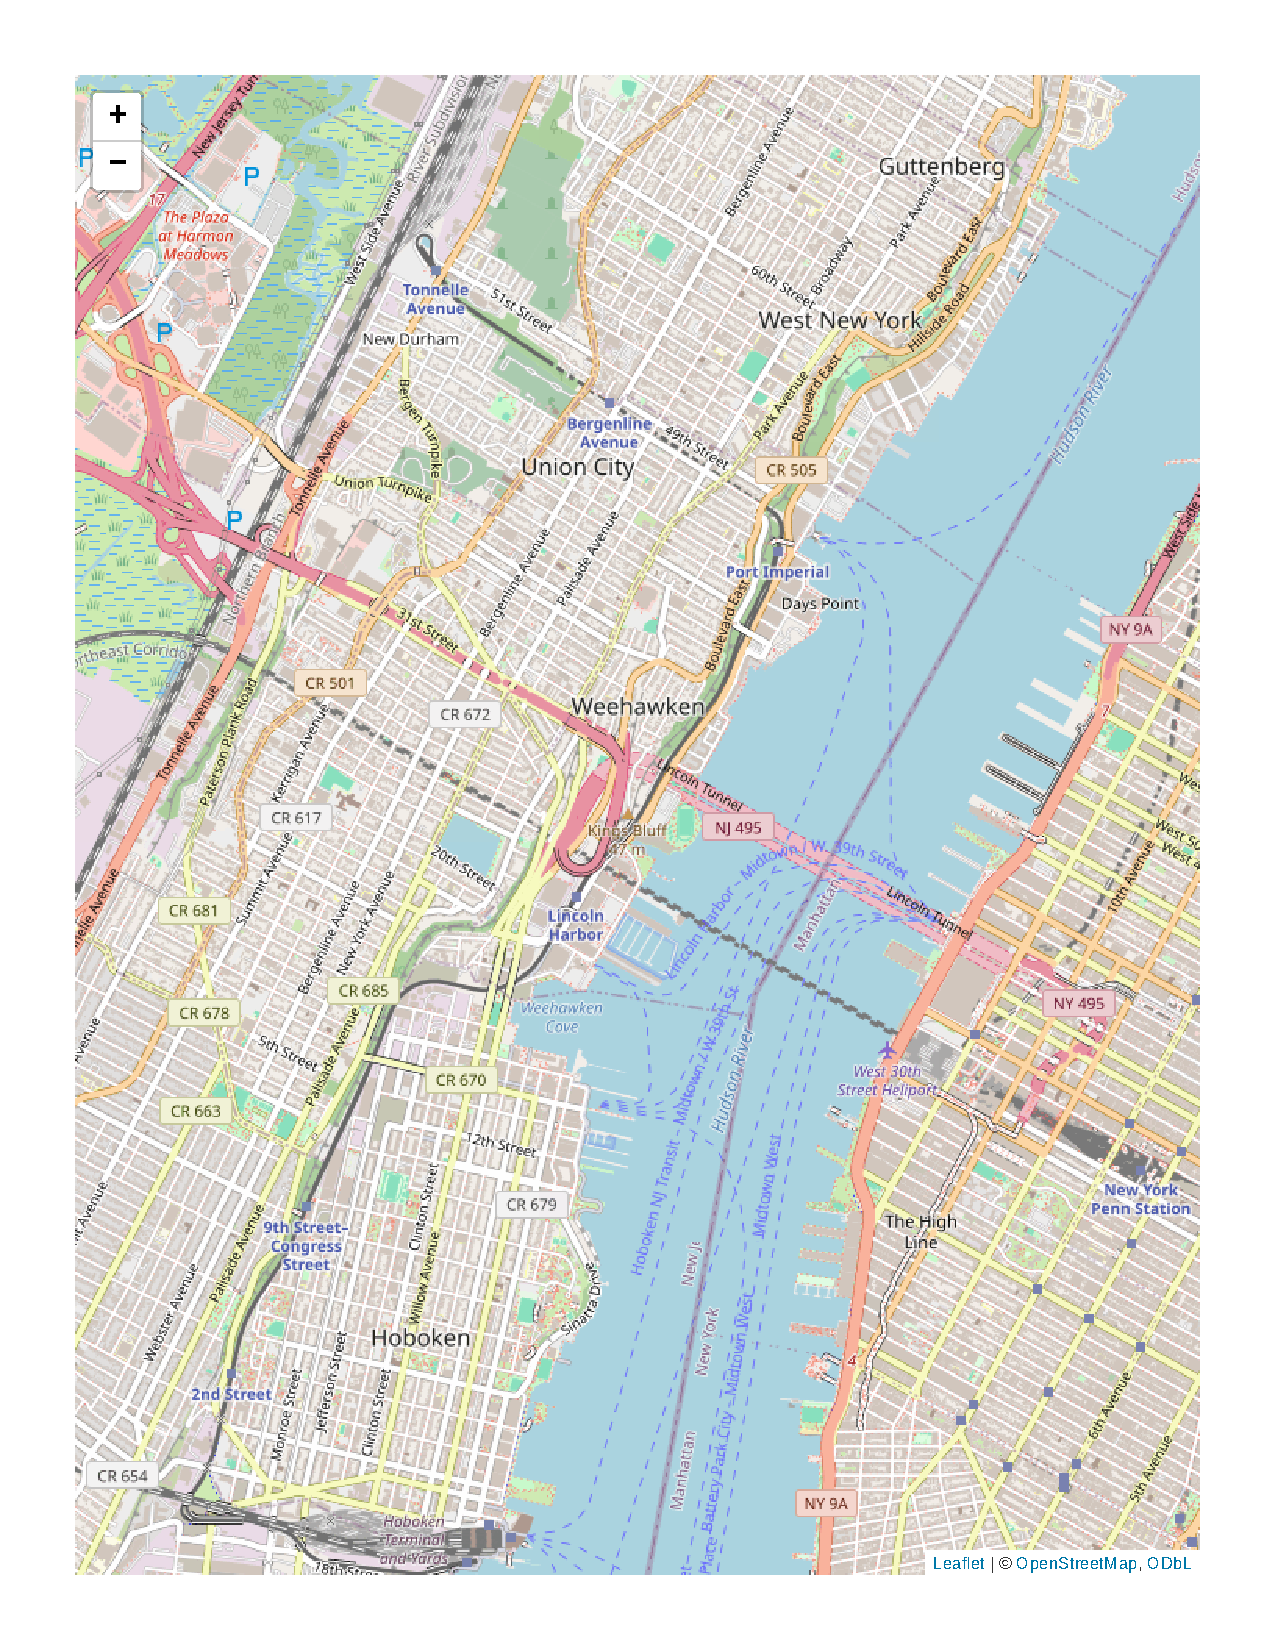
\includegraphics{andan-cluster_files/figure-pdf/manhattan-1.pdf}

Или майкопским --- тут вообще рай обожателя геометрии:

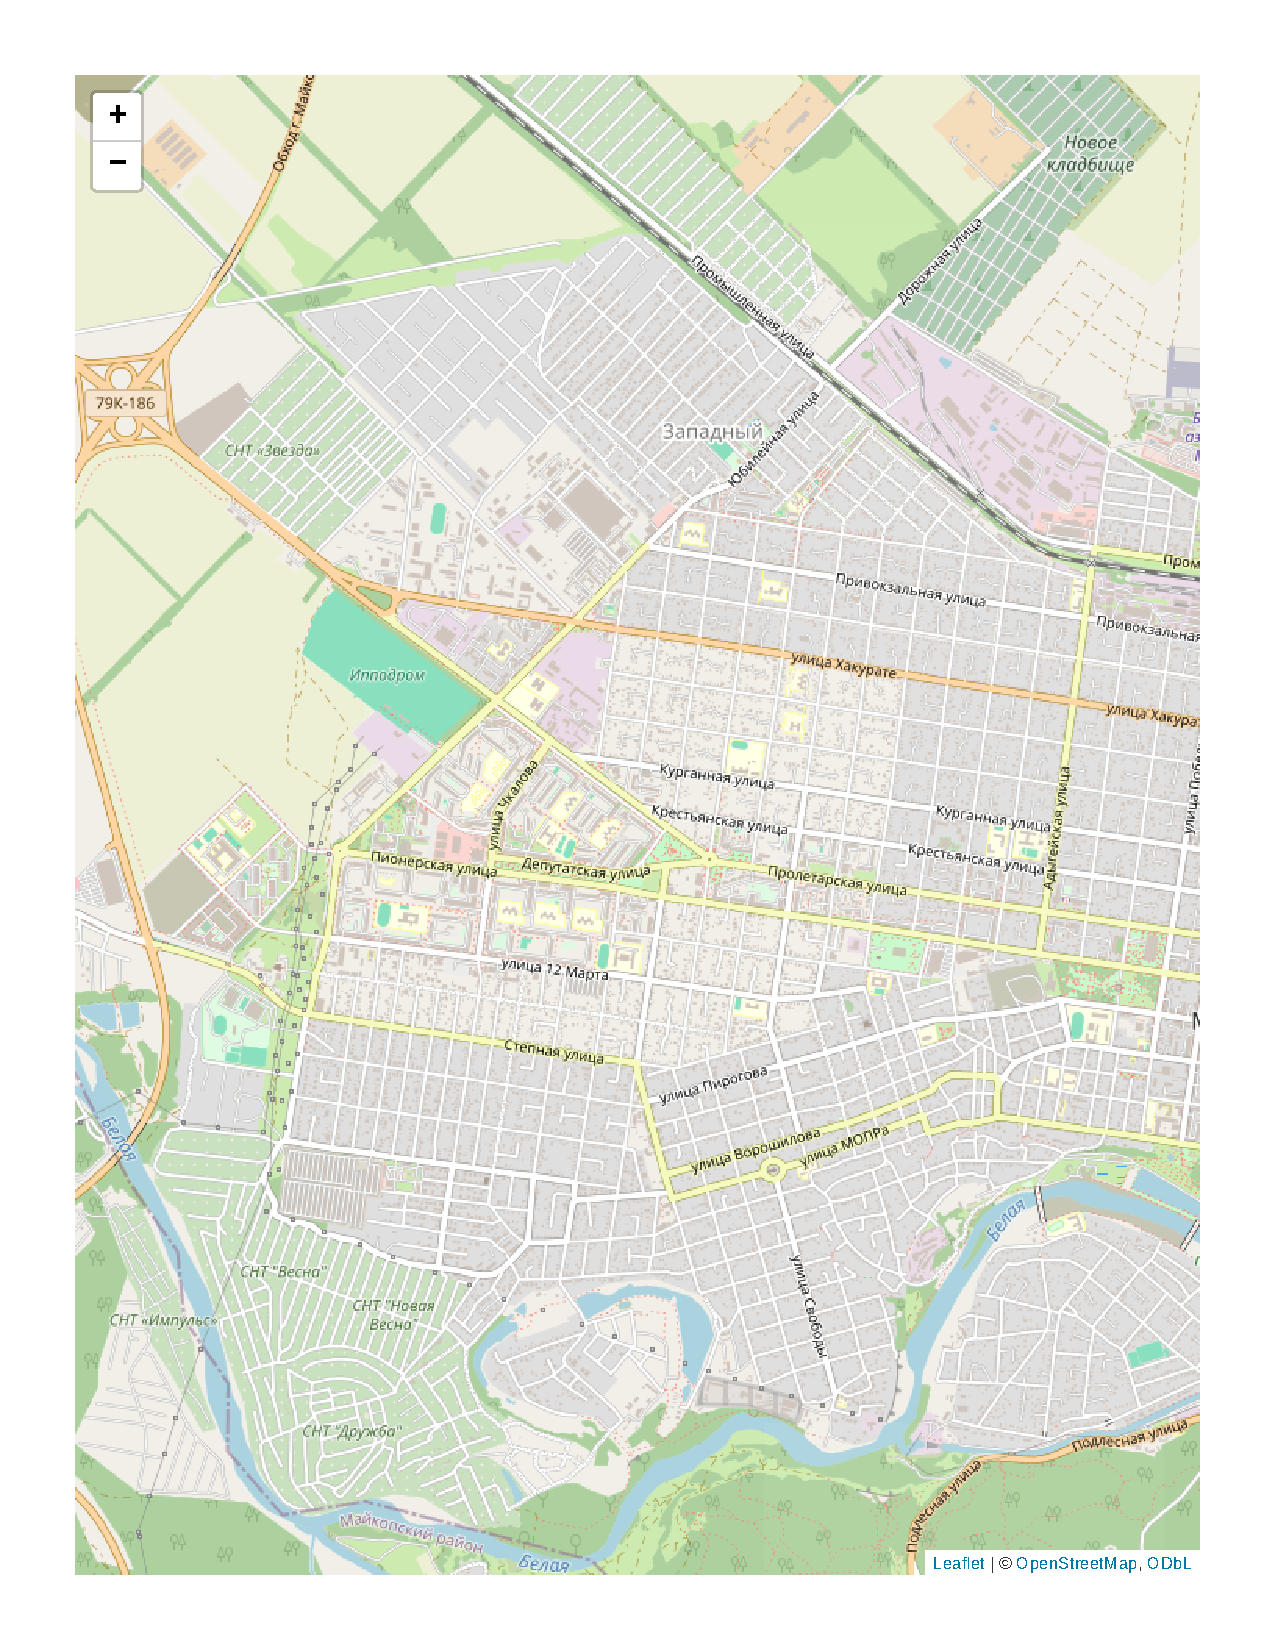
\includegraphics{andan-cluster_files/figure-pdf/maikop-1.pdf}

\bookmarksetup{startatroot}

\chapter{Линейный дискриминантный анализ}\label{andan-lda}

\bookmarksetup{startatroot}

\chapter{Анализ главных компонент}\label{andan-pca}

\bookmarksetup{startatroot}

\chapter{Анализ независимых компонент}\label{andan-ica}

\bookmarksetup{startatroot}

\chapter{Анализ скоррелированных компонент}\label{andan-cca}

\bookmarksetup{startatroot}

\chapter{Эксплораторный факторный анализ}\label{andan-efa}

\bookmarksetup{startatroot}

\chapter{Моделирование структурными уравнениями}\label{andan-sem}

\bookmarksetup{startatroot}

\chapter{Конфирматорный факторный анализ}\label{andan-cfa}

\bookmarksetup{startatroot}

\chapter{Путевой анализ}\label{andan-path}

\bookmarksetup{startatroot}

\chapter{Основы анализа временных рядов}\label{andan-timeseries}

\part{Анализ данных в R}

\bookmarksetup{startatroot}

\chapter{Описательные статистики в R}\label{randan-descriptives}

\bookmarksetup{startatroot}

\chapter{Сравнение средних в R}\label{randan-ttest}

\bookmarksetup{startatroot}

\chapter{Анализ категориальных данных в R}\label{randan-chisq}

\bookmarksetup{startatroot}

\chapter{Корреляционный анализ в R}\label{randan-corr}

\bookmarksetup{startatroot}

\chapter{Непараметрические методы анализа данных в
R}\label{randan-nonparam}

\bookmarksetup{startatroot}

\chapter{Общие линейные модели. Простая линейная регрессия в
R}\label{randan-simplelinear}

\bookmarksetup{startatroot}

\chapter{Множественная линейная регрессия в
R}\label{randan-multiplelinear}

\bookmarksetup{startatroot}

\chapter{Полиномиальная регрессия в R}\label{randan-polynomial}

\bookmarksetup{startatroot}

\chapter{Support Vector Regression в R}\label{randan-svr}

\bookmarksetup{startatroot}

\chapter{Регуляризованная регрессия в R}\label{randan-regreg}

\bookmarksetup{startatroot}

\chapter{Дисперсионный анализ в R}\label{randan-anova}

\bookmarksetup{startatroot}

\chapter{Ковариационный анализ в R}\label{randan-ancova}

\bookmarksetup{startatroot}

\chapter{Многомерный дисперсионный анализ в R}\label{randan-manova}

\bookmarksetup{startatroot}

\chapter{Деревья решений. Регрессия в R}\label{randan-treesreg}

\bookmarksetup{startatroot}

\chapter{Случайный лес. Регрессия в R}\label{randan-randforestreg}

\bookmarksetup{startatroot}

\chapter{Определение вида распределения переменной в
R}\label{randan-distributions}

\bookmarksetup{startatroot}

\chapter{Обобщенные линейные модели. Логистическая регрессия в
R}\label{randan-logreg}

\bookmarksetup{startatroot}

\chapter{Мультиномиальная логистическая регрессия в
R}\label{randan-multinomlogreg}

\bookmarksetup{startatroot}

\chapter{Пуассоновская регрессия в R}\label{randan-poissonreg}

\bookmarksetup{startatroot}

\chapter{Обобщенные аддитивные модели в R}\label{randan-gam}

\bookmarksetup{startatroot}

\chapter{Смешанные линейные модели в R}\label{randan-glmm}

\bookmarksetup{startatroot}

\chapter{Support Vector Machine}\label{andan-svm}

\bookmarksetup{startatroot}

\chapter{Деревья решений. Классификация в R}\label{randan-treesclass}

\bookmarksetup{startatroot}

\chapter{Случайный лес. Классификация в R}\label{randan-randforestclass}

\bookmarksetup{startatroot}

\chapter{Кластерный анализ в R}\label{randan-cluster}

\bookmarksetup{startatroot}

\chapter{Линейный дискриминантный анализ в R}\label{randan-lda}

\bookmarksetup{startatroot}

\chapter{Анализ главных компонент в R}\label{randan-pca}

\bookmarksetup{startatroot}

\chapter{Анализ независимых компонент в R}\label{randan-ica}

\bookmarksetup{startatroot}

\chapter{Анализ скоррелированных компонент в R}\label{randan-cca}

\bookmarksetup{startatroot}

\chapter{Эксплораторный факторный анализ в R}\label{randan-efa}

\bookmarksetup{startatroot}

\chapter{Моделирование структурными уравнениями в R}\label{randan-sem}

\bookmarksetup{startatroot}

\chapter{Конфирматорный факторный анализ в R}\label{randan-cfa}

\bookmarksetup{startatroot}

\chapter{Путевой анализ в R}\label{randan-path}

\bookmarksetup{startatroot}

\chapter{Основы анализа временных рядов в R}\label{randan-timeseries}

\part{Приложения}

\bookmarksetup{startatroot}

\chapter{Числа и железо}\label{appendix_numbers}

\emph{В ходе анализа данных мы непрерывно работаем с числами. Попробуем
разобраться, как они храняться в памяти компа, и почему}
\texttt{0.9\ +\ 0.5\ ==\ 1.4} \emph{далеко не во всех языках
програмирования даёт результат} \texttt{TRUE}.

\section{Целые числа}\label{integer_iron}

\subsection{Системы счисления}\label{number_systems}

\subsection{Перевод числа из одной системы счисления в
другую}\label{system_to_system}

\subsection{Целочисленные типы}\label{integer_types}

\section{Отрицательные числа}\label{negative_iron}

\subsection{Знаковые и беззнаковые типы}\label{unsigned_type}

\section{Числа с плавающей точкой}\label{float_iron}

\subsection{Экспоненциальная запись числа}\label{scientific_notation}

\subsection{Типы чисел c плавающей точкой}\label{float_types}

\bookmarksetup{startatroot}

\chapter{Строки и железо}\label{appendix_strings}

\bookmarksetup{startatroot}

\chapter{Килобайты}\label{appendix_kilobytes}

\bookmarksetup{startatroot}

\chapter{Память и процессор}\label{appendix_memory}

\bookmarksetup{startatroot}

\chapter{Языки программирования}\label{appendix_proglang}

\bookmarksetup{startatroot}

\chapter{Git}\label{appendix_git}

\section{Концепция
Git}\label{ux43aux43eux43dux446ux435ux43fux446ux438ux44f-git}

\section{Source Tree}\label{source-tree}

\section{CLI}\label{cli}

\subsection{\texorpdfstring{\texttt{git\ clone}}{git clone}}\label{git-clone}

\subsection{\texorpdfstring{\texttt{git\ status}}{git status}}\label{git-status}

\subsection{\texorpdfstring{\texttt{git\ diff}}{git diff}}\label{git-diff}

\subsection{\texorpdfstring{\texttt{git\ log}}{git log}}\label{git-log}

\subsection{\texorpdfstring{\texttt{git\ add}}{git add}}\label{git-add}

\subsection{\texorpdfstring{\texttt{git\ commit}}{git commit}}\label{git-commit}

\subsection{\texorpdfstring{\texttt{git\ push}}{git push}}\label{git-push}

\subsection{\texorpdfstring{\texttt{git\ pull}}{git pull}}\label{git-pull}

\subsection{\texorpdfstring{\texttt{git\ branch}}{git branch}}\label{git-branch}

\subsection{\texorpdfstring{\texttt{git\ checkout}}{git checkout}}\label{git-checkout}

\subsection{\texorpdfstring{\texttt{git\ config}}{git config}}\label{git-config}

\bookmarksetup{startatroot}

\chapter{Формулы}\label{formulas}

\section{Степени и корни}\label{formulas_power}

\subsection{Определения}\label{formulas_power_def}

\[
a^b \def \prod_{i=1}^b a_i
\]

\[
\sqrt[n]a \def b \Leftrightarrow b^n = a
\]

\subsection{Свойства}\label{formulas_power_identities}

\[a^n \cdot a^m = a^{n+m}\] \[\frac{a^n}{a^m} = a^{n-m}\]
\[(a^n)^m = a^{nm}\] \[a^0 = 1\] \[a^{-n}=\frac{1}{a^n}\]
\[(a \cdot b)^n = a^n \cdot b^n\]
\[\Big(\frac{a}{b}\Big)^n = \frac{a^n}{b^n}\]

\[a^{\frac{1}{n}}=\sqrt[n]{a}\] \[a^{\frac{m}{n}}=\sqrt[n]{a^m}\]
\[\sqrt[n]{a \cdot b} = \sqrt[n]{a} \cdot \sqrt[n]{b}\]
\[(a \cdot b)^{\frac{1}{n}} = a^{\frac{1}{n}} \cdot b^{\frac{1}{n}}\]
\[\sqrt[n]{\frac{a}{b}} = \frac{\sqrt[n]{a}}{\sqrt[n]{b}}\]
\[\Big(\frac{a}{b}\Big)^{\frac{1}{n}} = \frac{a^{\frac{1}{n}}}{b^{\frac{1}{n}}}\]

\[
x^n = a \Rightarrow x = 
\begin{cases}
\pm \sqrt[n]{a}, &\quad x \mod 2 = 0 \\ 
\sqrt[n]{a}, &\quad x \mod 2 = 1
\end{cases}
\]

\section{Логарифмы}\label{formulas_log}

\subsection{Определение}\label{formulas_log_def}

\[\log_b a \def c \Leftrightarrow a^c = b, a > 0, b > 0, b \neq 1\]

\subsection{Свойства}\label{formulas_log_identities}

\[\log_a a = 1\] \[\log_c(ab) = \log_c a + \log_c b\]
\[\log_c\Big(\frac{a}{b}\Big) = \log_c a - \log_c b\]

\[\log_c 1 = 0\] \[\log_c a^b = b \log_c a\]
\[\log_{c^b} a = \frac{1}{b} \log_c a\]

\section{Модуль}\label{formulas_abs}

\[
|a| = 
\begin{cases}
a, &a \geq 0 \\
-a, &a < 0
\end{cases}
\]

\[|x| \leq a \Rightarrow -a \leq x \leq a \Leftrightarrow x \in [-a, a]\]

\[|x| \geq a \Rightarrow x \leq -a \wedge x \geq a \Leftrightarrow x \in (-\infty, -a] \cup [a, +\infty)\]

\section{Производная}\label{formulas_deriv}

\subsection{Свойства производной}\label{formulas_deriv_props}

\[c' = 0, \, c = \const\] \[(Cu)' = Cu'\] \[(u + v)' = u' + v'\]
\[(uv)' = u'v + uv'\]
\[\Big( \frac{u}{v} \Big)' = \frac{u'v - uv'}{v^2}\]
\[\Big(u\big(v(x)\big)\Big)' = u'(v) \cdot v'(x)\]

\subsection{Производные элементарных
функций}\label{formulas_deriv_funcs}

\[(x^n)' = nx^{n-1}\] \[(a^x)' = a^x \ln a\] \[(e^x)' = e^x\]

\[(\log_a x)' = \frac{1}{x \ln a}\] \[(\ln_a x)' = \frac{1}{x}\]
\[(\sqrt{x})' = \frac{1}{2\sqrt{x}}\]

\[(\sin x)' = \cos x\] \[(\cos x)' = -\sin x\]

\[(\tan x)' = \frac{1}{\cos^2 x}\] \[(\cot x)' = \frac{1}{\sin^2 x}\]

\[(\arcsin x)' = \frac{1}{\sqrt{1 - x^2}}\]
\[(\arccos x)' = -\frac{1}{\sqrt{1 - x^2}}\]
\[(\arctan x)' = \frac{1}{1 + x^2}\]
\[(\text{arccot}\, x)' = -\frac{1}{1 + x^2}\]

\[(\sinh x)' = \cosh x\] \[(\cosh x)' = \sinh x\]
\[(\tanh x)' = \frac{1}{\cosh^2 x}\]
\[(\coth x)' = -\frac{1}{\sinh^2 x}\]

\section{Тригонометрия}\label{formulas_trig}

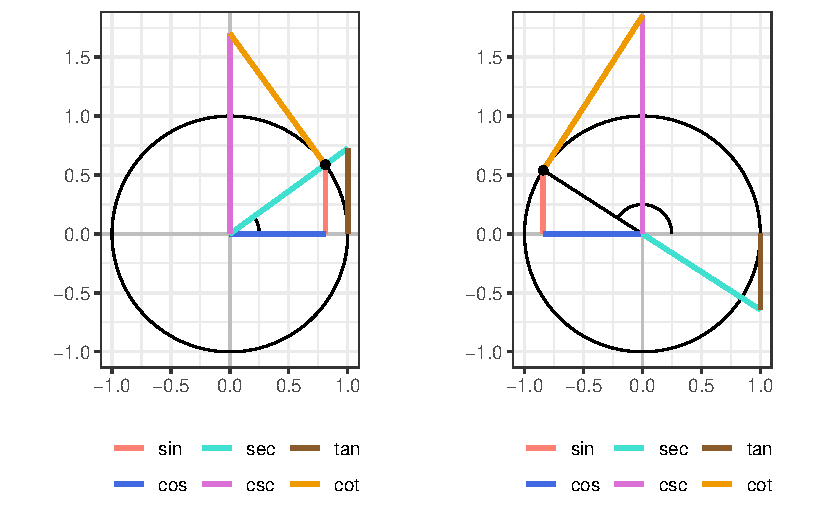
\includegraphics{appendix-formulas_files/figure-pdf/trig_circle-1.pdf}

\subsection{Производные тригонометрические функции}\label{trig_funs_def}

\[
\sec \alpha = \frac{1}{\cos \alpha} \qquad
\csc \alpha = \frac{1}{\sin \alpha} \qquad
\tan \alpha = \frac{\sin \alpha}{\cos \alpha} \qquad
\cot \alpha = \frac{\cos \alpha}{\sin \alpha}
\]

\subsection{Основное тригонометрическое
тождество}\label{trig_pythagorean_identities}

\[
\sin^2 \alpha + \cos^2 \alpha = 1
\]

\[
\sin \alpha = \pm \sqrt{1 - \cos^2 \alpha} \qquad \cos \alpha = \pm \sqrt{1 - \sin^2 \alpha}
\]

\[
1 + \cot^2 \alpha = \csc^2 \alpha \qquad
\tan^2 \alpha + 1 = \sec ^2 \alpha
\]

\[
\sec^2 \alpha + \csc^2 \alpha = \sec^2 \alpha \cdot \csc^2 \alpha
\]

\subsection{Отражения}\label{trig_reflections}

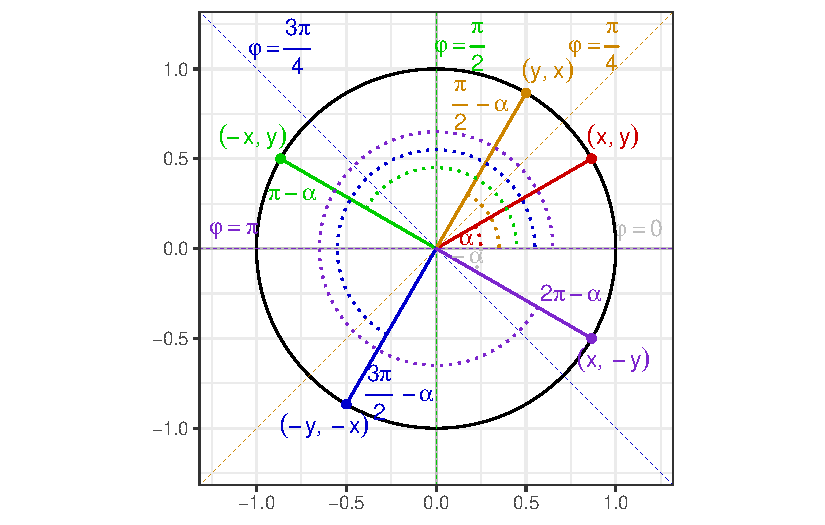
\includegraphics{appendix-formulas_files/figure-pdf/trig_reflections_circle-1.pdf}

\subsubsection{\texorpdfstring{Относительно
\(\varphi = 0\)}{Относительно \textbackslash varphi = 0}}\label{trig_reflections_0}

Выражает свойство чётности функции\footnote{Функция называется
  \emph{чётной}, если \(f(-x) = f(x)\), и нечётной, если
  \(f(-x) = -f(x)\).}.

\[\sin (-\alpha) = -\sin \alpha\] \[\tan (-\alpha) = -\tan \alpha\]
\[\sec (-\alpha) = \sec \alpha\]

\[\cos (-\alpha) = \cos \alpha\] \[\cot (-\alpha) = -\cot \alpha\]
\[\csc (-\alpha) = -\csc \alpha\]

\subsubsection{\texorpdfstring{Относительно
\(\varphi = \frac{\pi}{4}\)}{Относительно \textbackslash varphi = \textbackslash frac\{\textbackslash pi\}\{4\}}}\label{trig_reflections_pi4}

\[\sin (\frac{\pi}{2}-\alpha) = \cos \alpha\]
\[\tan \Big(\frac{\pi}{2}-\alpha\Big) = \cot \alpha\]
\[\sec \Big(\frac{\pi}{2}-\alpha\Big) = \csc \alpha\]

\[\cos \Big(\frac{\pi}{2}-\alpha\Big) = \sin \alpha\]
\[\cot \Big(\frac{\pi}{2}-\alpha\Big) = \tan \alpha\]
\[\csc \Big(\frac{\pi}{2}-\alpha\Big) = \sec \alpha\]

\subsubsection{\texorpdfstring{Относительно
\(\varphi = \frac{\pi}{2}\)}{Относительно \textbackslash varphi = \textbackslash frac\{\textbackslash pi\}\{2\}}}\label{trig_reflections_pi2}

\[\sin (\pi-\alpha) = \sin \alpha\] \[\tan (\pi-\alpha) = -\tan \alpha\]
\[\sec (\pi-\alpha) = -\sec \alpha\]

\[\cos (\pi-\alpha) = -\cos \alpha\]
\[\cot (\pi-\alpha) = -\cot \alpha\] \[\csc (\pi-\alpha) = \csc \alpha\]

\subsubsection{\texorpdfstring{Относительно
\(\varphi = \frac{3\pi}{4}\)}{Относительно \textbackslash varphi = \textbackslash frac\{3\textbackslash pi\}\{4\}}}\label{trig_reflections_3pi2}

\[\sin \Big(\frac{3\pi}{2}-\alpha\Big) = -\cos \alpha\]
\[\tan \Big(\frac{3\pi}{2}-\alpha\Big) = \cot \alpha\]
\[\sec \Big(\frac{3\pi}{2}-\alpha\Big) = -\csc \alpha\]

\[\cos \Big(\frac{3\pi}{2}-\alpha\Big) = -\sin \alpha\]
\[\cot \Big(\frac{3\pi}{2}-\alpha\Big) = \tan \alpha\]
\[\csc \Big(\frac{3\pi}{2}-\alpha\Big) = -\sec \alpha\]

\subsubsection{\texorpdfstring{Относительно
\(\varphi = \pi\)}{Относительно \textbackslash varphi = \textbackslash pi}}\label{trig_reflections_pi}

\[\sin (2\pi - \alpha) = -\sin \alpha = \sin (-\alpha)\]
\[\tan (2\pi - \alpha) = -\tan \alpha = \tan (-\alpha)\]
\[\sec (2\pi - \alpha) = \sec \alpha = \sec (-\alpha)\]

\[\cos (2\pi - \alpha) = \cos \alpha = \cos (-\alpha)\]
\[\cot (2\pi - \alpha) = -\cot \alpha = \cot (-\alpha)\]
\[\csc (2\pi - \alpha) = -\csc \alpha = \csc (-\alpha)\]

\subsection{Сдвиг}\label{trig_shift}

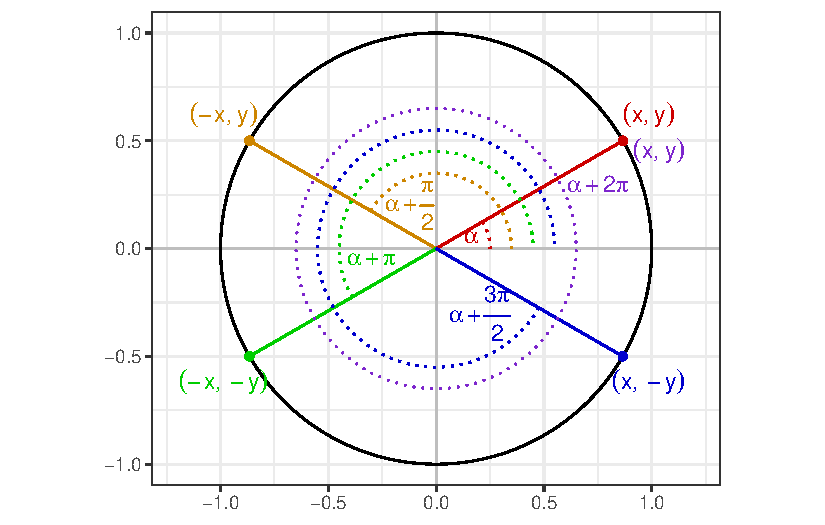
\includegraphics{appendix-formulas_files/figure-pdf/trig_shift_circle-1.pdf}

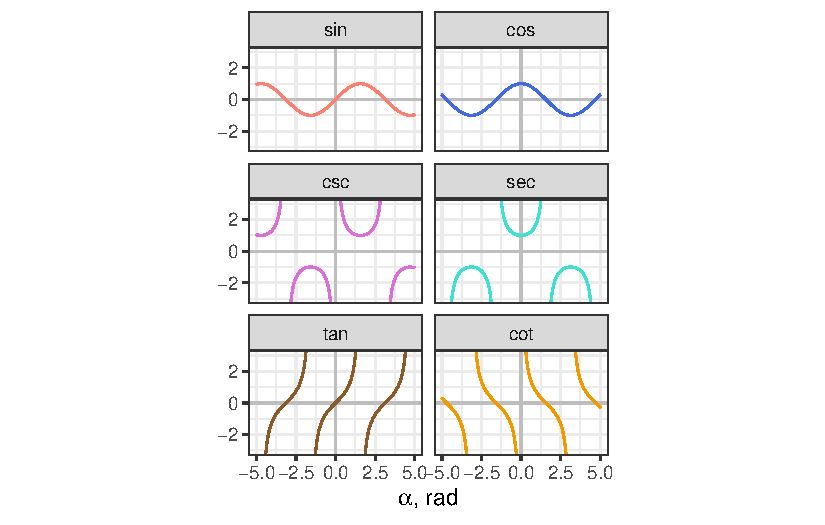
\includegraphics{appendix-formulas_files/figure-pdf/trig_shift_graphs-1.pdf}

Так как все тригонометрические функции периодические, результат сдвига
функции определяется её периодом. Для функций \(\sin, \cos, \sec\) и
\(\csc\) период равен \(2\pi\). Для \(\tan\) и \(\cot\) он составляет
\(\pi\).

\subsubsection{На четверть периода}\label{trig_shift_by_one_quarter}

\[\sin \Big(\alpha \pm \frac{\pi}{2}\Big) = \pm\cos \alpha\]
\[\tan \Big(\alpha \pm \frac{\pi}{4}\Big) = \frac{\tan \alpha \pm 1}{1 \mp \tan \alpha}\]
\[\sec \Big(\alpha \pm \frac{\pi}{2}\Big) = \mp \csc \alpha\]

\[\cos \Big(\alpha \pm \frac{\pi}{2}\Big) = \mp \sin \alpha\]
\[\cot \Big(\alpha \pm \frac{\pi}{4}\Big) = \frac{\cot \alpha \mp 1}{1 \pm \cot \alpha}\]
\[\csc \Big(\alpha \pm \frac{\pi}{2}\Big) = \pm \sec \alpha\]

\subsubsection{На половину периода}\label{trig_shift_by_half}

\[\sin (\alpha + \pi) = -\sin \alpha\]
\[\tan \Big(\alpha + \frac{\pi}{2}\Big) = -\cot \alpha\]
\[\sec (\alpha + \pi) = -\sec \alpha\]

\[\cos (\alpha + \pi) = -\cos \alpha\]
\[\cot \Big(\alpha + \frac{\pi}{2}\Big) = -\tan \alpha\]
\[\csc (\alpha + \pi) = -\csc \alpha\]

\subsubsection{На полный период}\label{trig_shift_by_full}

\[\sin (\alpha + 2\pi) = \sin \alpha\]
\[\tan (\alpha + \pi) = \tan \alpha\]
\[\sec (\alpha + 2\pi) = \sec \alpha\]

\[\cos (\alpha + 2\pi) = \cos \alpha\]
\[\cot (\alpha + \pi) = \cot \alpha\]
\[\csc (\alpha + 2\pi) = \csc \alpha\]

\subsection{Соотношение знаков}\label{trig_sgn}

\[
\sgn \sin \alpha = \sgn \csc \alpha \qquad \sgn \cos \alpha = \sgn \sec \alpha
\] \[
\sgn \tan \alpha = \sgn \cot \alpha
\]

\subsection{Функции суммы с разности аргументов}\label{trig_angle_sum}

\[
\sin (\alpha \pm \beta) = \sin \alpha \cos \beta \pm \cos \alpha \sin \beta
\]

\[
\cos (\alpha \pm \beta) = \cos \alpha \cos \beta \mp \sin \alpha \sin \beta
\]

\[
\tan (\alpha \pm \beta) = \frac{\tan \alpha \pm \tan \beta}{1 \mp \tan \alpha \tan \beta}
\]

\[
\cot (\alpha \pm \beta) = \frac{\cot \alpha \cot \beta \mp 1}{\cot \beta \pm \cot \alpha}
\] \[
\sec (\alpha \pm \beta) = \frac{\sec \alpha \sec \beta \csc \alpha \csc \beta}{\csc \alpha \csc \beta \mp \sec \alpha \sec \beta}
\]

\[
\csc (\alpha \pm \beta) = \frac{\sec \alpha \sec \beta \csc \alpha \csc \beta}{\sec \alpha \csc \beta \pm \sec \alpha \sec \beta}
\]

\subsection{Формулы двойного аргумента}\label{trig_double_arg}

\[
\sin 2\alpha = 2\sin \alpha \cos \alpha = (\sin \alpha + \cos \alpha)^2 -1 = \frac{2\tan \alpha}{1 + \tan^2 \alpha}
\]

\[
\cos 2\alpha = \cos^2 \alpha - \sin^2 \alpha = 2\cos^2 \alpha - 1 = 1 - 2\sin^2 \alpha = \frac{1 - \tan^2 \alpha}{1 + \tan^2 \alpha}
\]

\[
\tan 2\alpha = \frac{2\tan \alpha}{1 - \tan^2 \alpha}
\]

\[
\cot 2\alpha = \frac{\cot^2 \alpha - 1}{2 \cot \alpha} = \frac{1 - \tan^2 \alpha}{2 \tan \alpha}
\]

\[
\sec 2\alpha = \frac{\sec^2 \alpha}{2 - \sec^2 \alpha} = \frac{1 + \tan^2 \alpha}{1 - \tan^2 \alpha}
\]

\[
\csc 2\alpha = \frac{\sec \alpha \csc \alpha}{2} = \frac{1 + \tan^2 \alpha}{2 \tan \alpha}
\]

\subsection{Формулы тройного аргумента}\label{trig_triple_arg}

\[
\sin 3\alpha = 3\sin \alpha - 4 \sin^3 \alpha = 4\sin \alpha \sin \Big( \frac{\pi}{3} - \alpha\Big) \sin \Big( \frac{\pi}{3} + \alpha \Big)
\]

\[
\cos 3\alpha = 4\cos^3 \alpha - 3 \cos \alpha = 4\cos \alpha \cos \Big(\frac{\pi}{3} - \alpha\Big) \cos \Big(\frac{\pi}{3} + \alpha\Big)
\]

\[
\tan 3\alpha = \frac{3\tan \alpha - \tan^3 \alpha}{1 - 3\tan^2 \alpha} = \tan \alpha \tan \Big( \frac{\pi}{3} - \alpha \Big) \tan \Big(\frac{\pi}{3} + \alpha \Big)
\]

\[
\cot 3\alpha = \frac{3 \cot \alpha - \cot^3 \alpha}{1 - 3\cot^2 \alpha}
\]

\[
\sec 3\alpha = \frac{\sec^3 \alpha}{4 - 3\sec^2 \alpha}
\]

\[
\csc 3\alpha = \frac{\csc^3 \alpha}{3\csc^2 \alpha -4}
\]

\subsection{Формулы половинного аргумента}\label{trig_half_arg}

\[
\sin \frac{\alpha}{2} = \sgn \Big(\sin \frac{\alpha}{2} \Big) \sqrt{\frac{1 - \cos \alpha}{2}}
\]

\[
\cos \frac{\alpha}{2} = \sgn \Big( \cos \frac{\alpha}{2} \Big) \sqrt{\frac{1 + \cos \alpha}{2}}
\]

\[
\tan \frac{\alpha}{2} = \frac{1 - \cos\alpha}{\sin \alpha} = \frac{\sin \alpha}{1 + \cos \alpha} = \csc \alpha - \cot \alpha = \frac{\tan \alpha}{1 + \sec \alpha} = \sgn (\sin \alpha) \sqrt{\frac{1 - \cos \alpha}{1 + \cos \alpha}}
\]

\[
\cot \frac{\alpha}{2} = \frac{1 + \cos \alpha}{\sin \alpha} = \frac{\sin \alpha}{1 - \cos \alpha} = \csc \alpha + \cot \alpha = \sgn(\sin \alpha) \sqrt{\frac{1 + \cos \alpha}{1 - \cos{\alpha}}}
\]

\[
\sec \frac{\alpha}{2} = \sgn \Big( \cos \frac{\alpha}{2} \Big) \sqrt{\frac{2}{1 + \cos \alpha}}
\]

\[
\csc \frac{\alpha}{2} = \sgn \Big( \sin \frac{\alpha}{2}  \Big) \sqrt{\frac{2}{1 - \cos \alpha}}
\]

\subsection{Формулы понижения степени}\label{trig_power_reduction}

\[
\sin^2 \alpha = \frac{1 - \cos 2\alpha}{2}
\]

\[
\cos^2 \alpha = \frac{1 + \cos 2\alpha}{2}
\]

\[
\tan^2 \alpha = \frac{1 - \cos 2\alpha}{1 + \cos 2\alpha}
\]

\[
\cot^2 \alpha = \frac{1 + \cos 2\alpha}{1 - \cos 2\alpha}
\]

\[
\sec^2 \alpha = \frac{2}{1 + \cos 2\alpha}
\]

\[
\csc^2 \alpha = \frac{2}{1 - \cos 2\alpha}
\]

\subsection{Преобразование произведения в сумму}\label{trig_prod_to_sum}

\[
\cos \alpha \cos \beta = \frac{\cos (\alpha - \beta) + \cos (\alpha + \beta)}{2}
\]

\[
\sin \alpha \sin \beta = \frac{\cos (\alpha - \beta) - \cos (\alpha + \beta)}{2}
\]

\[
\sin \alpha \cos \beta = \frac{\sin (\alpha + \beta) + \sin (\alpha - \beta)}{2}
\]

\[
\cos \alpha \sin \beta = \frac{\sin (\alpha + \beta) - \sin (\alpha - \beta)}{2}
\]

\[
\tan \alpha \tan \beta = \frac{\cos (\alpha - \beta) - \cos (\alpha + \beta)}{\cos (\alpha - \beta) + \cos (\alpha + \beta)}
\]

\[
\tan \alpha \cot \beta = \frac{\sin (\alpha + \beta) + \sin (\alpha - \beta)}{\sin (\alpha + \beta) - \sin (\alpha - \beta)}
\]

\subsection{Преобразование суммы в произведение}\label{trig_sum_to_prod}

\[
\sin \alpha \pm \sin \beta = 2 \sin \Big(\frac{\alpha \pm \beta}{2}\Big) \cos \Big(\frac{\alpha \mp \beta}{2}\Big)
\]

\[
\cos \alpha + \cos \beta = 2 \cos \Big(\frac{\alpha + \beta}{2}\Big) \cos \Big(\frac{\alpha - \beta}{2}\Big)
\]

\[
\cos \alpha - \cos \beta = -2 \sin \Big(\frac{\alpha + \beta}{2}\Big) \sin \Big(\frac{\alpha - \beta}{2}\Big)
\]

\[
\tan \alpha \pm \tan \beta = \frac{sin(\alpha + \beta)}{\cos \alpha \cos \beta}
\]

\bookmarksetup{startatroot}

\chapter{Дизайн}\label{ux434ux438ux437ux430ux439ux43d}

\section{Цвет}\label{ux446ux432ux435ux442}

\section{Изображения}\label{ux438ux437ux43eux431ux440ux430ux436ux435ux43dux438ux44f}

\section{Шрифты}\label{ux448ux440ux438ux444ux442ux44b}

\bookmarksetup{startatroot}

\chapter*{Источники}\label{ux438ux441ux442ux43eux447ux43dux438ux43aux438}
\addcontentsline{toc}{chapter}{Источники}

\markboth{Источники}{Источники}

\printbibliography[heading=none]


\backmatter


\end{document}
